% Options for packages loaded elsewhere
\PassOptionsToPackage{unicode}{hyperref}
\PassOptionsToPackage{hyphens}{url}
%
\documentclass[
]{article}
\usepackage{amsmath,amssymb}
\usepackage{lmodern}
\usepackage{iftex}
\ifPDFTeX
  \usepackage[T1]{fontenc}
  \usepackage[utf8]{inputenc}
  \usepackage{textcomp} % provide euro and other symbols
\else % if luatex or xetex
  \usepackage{unicode-math}
  \defaultfontfeatures{Scale=MatchLowercase}
  \defaultfontfeatures[\rmfamily]{Ligatures=TeX,Scale=1}
\fi
% Use upquote if available, for straight quotes in verbatim environments
\IfFileExists{upquote.sty}{\usepackage{upquote}}{}
\IfFileExists{microtype.sty}{% use microtype if available
  \usepackage[]{microtype}
  \UseMicrotypeSet[protrusion]{basicmath} % disable protrusion for tt fonts
}{}
\makeatletter
\@ifundefined{KOMAClassName}{% if non-KOMA class
  \IfFileExists{parskip.sty}{%
    \usepackage{parskip}
  }{% else
    \setlength{\parindent}{0pt}
    \setlength{\parskip}{6pt plus 2pt minus 1pt}}
}{% if KOMA class
  \KOMAoptions{parskip=half}}
\makeatother
\usepackage{xcolor}
\usepackage[margin=1in]{geometry}
\usepackage{longtable,booktabs,array}
\usepackage{calc} % for calculating minipage widths
% Correct order of tables after \paragraph or \subparagraph
\usepackage{etoolbox}
\makeatletter
\patchcmd\longtable{\par}{\if@noskipsec\mbox{}\fi\par}{}{}
\makeatother
% Allow footnotes in longtable head/foot
\IfFileExists{footnotehyper.sty}{\usepackage{footnotehyper}}{\usepackage{footnote}}
\makesavenoteenv{longtable}
\usepackage{graphicx}
\makeatletter
\def\maxwidth{\ifdim\Gin@nat@width>\linewidth\linewidth\else\Gin@nat@width\fi}
\def\maxheight{\ifdim\Gin@nat@height>\textheight\textheight\else\Gin@nat@height\fi}
\makeatother
% Scale images if necessary, so that they will not overflow the page
% margins by default, and it is still possible to overwrite the defaults
% using explicit options in \includegraphics[width, height, ...]{}
\setkeys{Gin}{width=\maxwidth,height=\maxheight,keepaspectratio}
% Set default figure placement to htbp
\makeatletter
\def\fps@figure{htbp}
\makeatother
\setlength{\emergencystretch}{3em} % prevent overfull lines
\providecommand{\tightlist}{%
  \setlength{\itemsep}{0pt}\setlength{\parskip}{0pt}}
\setcounter{secnumdepth}{-\maxdimen} % remove section numbering
\newlength{\cslhangindent}
\setlength{\cslhangindent}{1.5em}
\newlength{\csllabelwidth}
\setlength{\csllabelwidth}{3em}
\newlength{\cslentryspacingunit} % times entry-spacing
\setlength{\cslentryspacingunit}{\parskip}
\newenvironment{CSLReferences}[2] % #1 hanging-ident, #2 entry spacing
 {% don't indent paragraphs
  \setlength{\parindent}{0pt}
  % turn on hanging indent if param 1 is 1
  \ifodd #1
  \let\oldpar\par
  \def\par{\hangindent=\cslhangindent\oldpar}
  \fi
  % set entry spacing
  \setlength{\parskip}{#2\cslentryspacingunit}
 }%
 {}
\usepackage{calc}
\newcommand{\CSLBlock}[1]{#1\hfill\break}
\newcommand{\CSLLeftMargin}[1]{\parbox[t]{\csllabelwidth}{#1}}
\newcommand{\CSLRightInline}[1]{\parbox[t]{\linewidth - \csllabelwidth}{#1}\break}
\newcommand{\CSLIndent}[1]{\hspace{\cslhangindent}#1}
\ifLuaTeX
  \usepackage{selnolig}  % disable illegal ligatures
\fi
\IfFileExists{bookmark.sty}{\usepackage{bookmark}}{\usepackage{hyperref}}
\IfFileExists{xurl.sty}{\usepackage{xurl}}{} % add URL line breaks if available
\urlstyle{same} % disable monospaced font for URLs
\hypersetup{
  pdftitle={The effect of network structure on language variability},
  pdfauthor={My name {[}myemailaddres{]}, Collaborators Names},
  hidelinks,
  pdfcreator={LaTeX via pandoc}}

\title{The effect of network structure on language variability}
\usepackage{etoolbox}
\makeatletter
\providecommand{\subtitle}[1]{% add subtitle to \maketitle
  \apptocmd{\@title}{\par {\large #1 \par}}{}{}
}
\makeatother
\subtitle{Full statistical analysis and plots}
\author{My name {[}myemailaddres{]}, Collaborators Names}
\date{Wed Mar 20 11:17:24 2024}

\begin{document}
\maketitle

{
\setcounter{tocdepth}{6}
\tableofcontents
}
\hypertarget{introduction}{%
\section{INTRODUCTION}\label{introduction}}

This \texttt{HTML} document contains all the results and plots
supporting the paper \textbf{network structure shapes languages:
disentangling the factors driving variation in communicative agents}.
All the data and scripts needed to reproduce this document are available
in the \href{https://github.com/mathjoss/NetworkStructure_ABM}{GitHub}
repository.

\hypertarget{typographic-conventions}{%
\subsection{Typographic conventions}\label{typographic-conventions}}

This \texttt{HTML} document uses the following font and color
conventions:

\begin{itemize}
\tightlist
\item
  variables' name are represented using \emph{italic text}
\item
  emphasis is represented using \textbf{bold text}
\item
  software or programming concepts (e.g., applications, packages or
  function names) are represented using \texttt{fixed\ font\ text}
\item
  hyperlinks to sections of this document and to external resources on
  the web are represented as \protect\hyperlink{introduction}{link to
  the Introduction} or \href{https://www.r-project.org/}{link to R
  project's website}
\end{itemize}

\hypertarget{software-and-hardware-info}{%
\subsection{Software and hardware
info}\label{software-and-hardware-info}}

The full information about the version of \texttt{R} (R Core Team,
2022). The packages used to obtain this \texttt{html} file can be seen
when opening the corresponding \texttt{Rmarkdown} file.

To perform the simulations, we used two different machines:

\begin{itemize}
\tightlist
\item
  Latitude 7400, DEll, with a processor Intel64 Family 6 Model 142
  Stepping 12 GenuineIntel, x64bits, 16.0 Go RAM. R was used with
  version 4.2.1 and 4.3.0
\item
  PO145, with a processor Intel(R) Core(TM) i5-8365U CPU @ 1.60GHz 1.90
  GHz, x64bits, and 16.0 Go RAM. R was used with version 4.2.1.
\end{itemize}

\hypertarget{data}{%
\section{DATA}\label{data}}

For more information on the model, refer to the main paper.

\hypertarget{the-procedure}{%
\subsection{The procedure}\label{the-procedure}}

We conducted three types of simulations:

\begin{itemize}
\item
  \emph{DATASET 1}. In the first, we \textbf{systematically compared two
  sets of networks differing in exactly one metric}.
\item
  \emph{DATASET 2}. In the second, we used other datasets (with
  automatically generated random, scale-free, and small-world networks
  using a wide range of parameters) to complement these results and look
  at:

  \begin{itemize}
  \tightlist
  \item
    the \textbf{correlations} between the different metrics
  \item
    the \textbf{relative contribution} of the metrics by applying
    different types of models (machine learning models, such as random
    forests and support vector machines, as well as linear regression)
    using the different metrics normalized as predictors, to understand
    what metrics are the most important. These models help understand
    the relative contribution of each of these metrics in several
    network types. We expect to reach similar conclusions between
    network types and between methods.
  \end{itemize}
\item
  \emph{DATASET 3}. In the third, we looked at the language value
  \textbf{and} variation in heterogeneous populations (where some agents
  are locally biased) in all types of networks.
\end{itemize}

\hypertarget{step-1-generating-datasets-using-netlogo-program}{%
\subsection{Step 1: generating datasets using Netlogo
program}\label{step-1-generating-datasets-using-netlogo-program}}

The Netlogo program is available in the \emph{GitHub} repository
associated to this Supplementary Materials (see my
\href{https://github.com/mathjoss/NetworkStructure_ABM}{github} under
the name \texttt{Netlogo\_program\_dirichlet.nlogo}. This is an
extension of the Netlogo program available in our previous paper
\href{https://www.frontiersin.org/journals/psychology/articles/10.3389/fpsyg.2021.626118/full}{``Interindividual
variation refuses to go away: a Bayesian computer model of language
change in communicative networks''} (2021) published in \emph{Frontiers
in Psychology}, and available in the Supplementary Materials of this
paper \href{https://github.com/mathjoss/bayes-in-network}{here}. While
the model is the same, a few functions have been added (for example, it
is now possible to study multinomial language features).

To understand how to use our Netlogo code and parameters, please refer
to the Netlogo guide, a pdf file that can be found in the same
\href{https://github.com/mathjoss/NetworkStructure_ABM}{github} folder
(see \texttt{appendix\_netlogo.pdf} file)

These files are stored in a \texttt{Raw} folder. They have the following
name: \texttt{DN\_typesimulation\_networktype}:

\begin{itemize}
\tightlist
\item
  \texttt{N} can take the values \emph{1}, \emph{2}, or \emph{3}
  depending on the dataset number
\item
  \texttt{typesimulation} can take the values \emph{continuous} or
  \emph{multinomial} depending on the language studied
\item
  \texttt{networktype} can take the values \emph{scalefree},
  \emph{smallworld}, or \emph{random} based on the network used to
  generate the simulations.
\end{itemize}

For example, a file \texttt{D1\_dirichlet\_random.csv} present in the
folder \texttt{Raw} is the raw file obtained from Netlogo (using the
code called \texttt{D1\_dir\_random} in Behavioral Space), and includes
data obtained using \emph{random} networks, a \emph{multinomial}
language, for the \emph{dataset 1} (comparing sets of networks).

\hypertarget{parameters}{%
\subsubsection{Parameters}\label{parameters}}

Below are the specific parameters used to generate networks on Netlogo.

In Dataset 1, we conducted 100 replications for each combination of
parameters. In Dataset 2, we generated 900 networks for each network
type. This entailed 10 replications per combination for random networks,
5 replications per combination for small-world networks, and 100
replications per combination for scale-free networks. This choice was
guided by the aim to maintain models with a similar amount of data.
However, it is important to note that we also tried to study models with
100 replications for each combination of parameters within each network
type (so much more data for small-world compared t scale-free networks),
but this change did not impact any of our conclusions.

For \emph{scale-free} networks:

\begin{longtable}[]{@{}lll@{}}
\toprule()
Dataset number & Size network & Init value Dirichlet \\
\midrule()
\endhead
Dataset 1 & 50; 100 & 0; 5; 20 \\
Dataset 2 & 50; 150; 300 & 0; 5; 20 \\
Dataset 3 & 150 & 0; 5; 20 \\
\bottomrule()
\end{longtable}

For \emph{random} networks:

\begin{longtable}[]{@{}
  >{\raggedright\arraybackslash}p{(\columnwidth - 6\tabcolsep) * \real{0.2174}}
  >{\raggedright\arraybackslash}p{(\columnwidth - 6\tabcolsep) * \real{0.2609}}
  >{\raggedright\arraybackslash}p{(\columnwidth - 6\tabcolsep) * \real{0.2609}}
  >{\raggedright\arraybackslash}p{(\columnwidth - 6\tabcolsep) * \real{0.2609}}@{}}
\toprule()
\begin{minipage}[b]{\linewidth}\raggedright
Dataset number
\end{minipage} & \begin{minipage}[b]{\linewidth}\raggedright
Size network
\end{minipage} & \begin{minipage}[b]{\linewidth}\raggedright
Connection probability
\end{minipage} & \begin{minipage}[b]{\linewidth}\raggedright
Init value Dirichlet
\end{minipage} \\
\midrule()
\endhead
Dataset 1 & 50; 100 & 0.06; 0.24; 0.2;5 0.26 & 0; 5; 20 \\
Dataset 2 & 50; 150; 300 & 0.05; 0.15; 0.25; 0.35; 0.45; 0.55; 0.65;
0.75; 0.85; 0.95 & 0; 5; 20 \\
Dataset 3 & 150 & 0.08 & 0; 5; 20 \\
\bottomrule()
\end{longtable}

For \emph{small-world} networks:

\begin{longtable}[]{@{}
  >{\raggedright\arraybackslash}p{(\columnwidth - 8\tabcolsep) * \real{0.1724}}
  >{\raggedright\arraybackslash}p{(\columnwidth - 8\tabcolsep) * \real{0.2069}}
  >{\raggedright\arraybackslash}p{(\columnwidth - 8\tabcolsep) * \real{0.2069}}
  >{\raggedright\arraybackslash}p{(\columnwidth - 8\tabcolsep) * \real{0.2069}}
  >{\raggedright\arraybackslash}p{(\columnwidth - 8\tabcolsep) * \real{0.2069}}@{}}
\toprule()
\begin{minipage}[b]{\linewidth}\raggedright
Dataset number
\end{minipage} & \begin{minipage}[b]{\linewidth}\raggedright
Size network
\end{minipage} & \begin{minipage}[b]{\linewidth}\raggedright
Number neighbors
\end{minipage} & \begin{minipage}[b]{\linewidth}\raggedright
Rewiring probability
\end{minipage} & \begin{minipage}[b]{\linewidth}\raggedright
Init value Dirichlet
\end{minipage} \\
\midrule()
\endhead
Dataset 1 & 150 & 24 & 0.1; 0.9 & 0; 5; 20 \\
Dataset 2 & 50 150 & 2; 4; 8; 24 & 0.1; 0.3; 0.5; 0.7; 0.9 & 0 5 20 \\
Dataset 3 & 150 & 2 & 0.1; 0.9 & 0; 5; 20 \\
\bottomrule()
\end{longtable}

\hypertarget{note-on-initial-language-exposure-terminology}{%
\subsubsection{Note on Initial language exposure
terminology}\label{note-on-initial-language-exposure-terminology}}

The value for initial language exposure (which we refer here as
\emph{init\_lang\_exp}) tells the number of utterance that have been
heard after the agent is born. Since the agents are born with a vector =
{[}1, 1, 1, 1, 1, 1, 1, 1, 1, 1{]}, then their value in \(u_4\) becomes
6 (5+1) or 21 (20+1).

In the datasets, this variable has three modalities:

\begin{itemize}
\tightlist
\item
  \emph{init\_lang\_exp = 0} (so \(u_4\) at first = 1, similar to other
  values of the Dirichlet parameters): we call this condition
  \textbf{without} initial language exposure. In the paper, we refer to
  this situation as \textbf{language emergence} scenario.
\item
  \emph{init\_lang\_exp = 5} (so \(u_4\) at first = 6, contrary to other
  Dirichlet values which = 1): we call this condition \textbf{with
  (weak)} initial language exposure. In the paper, we refer to this
  situation as \textbf{language change} scenario.
\item
  \emph{init\_lang\_exp = 20} (so \(u_4\) at first = 21, contrary to
  other Dirichlet values which = 1): we call this condition \textbf{with
  (strong)} initial language exposure. In the paper, we do not refer to
  this condition, but that it is also a scenario of language change.
\end{itemize}

In these Supplementary Materials, we preferentially refer to this
variable with the modalities ``Without'', ``With (weak)'', and ``With
(strong)'' (instead of language change and emergence) because it allows
us to contrast between the two language change conditions (weak:
\(u_4\)=6 and strong: \(u_4\)=21).

\hypertarget{step-2-cleaning-netlogo-output-files}{%
\subsection{Step 2: cleaning netlogo output
files}\label{step-2-cleaning-netlogo-output-files}}

After we performed the analysis in Netlogo, we obtained files which
often contain thousands of simulations. Thus, these files are
\textbf{very heavy} and hard to read, containing many unecessary
informations (useless column, etc). (For example, for each network, we
stored the final value of the Dirichlet vector for all agents!)

We used \textbf{another Rmarkdown file} to clean this data (see
\texttt{CleanData.RmD} in the
\href{https://github.com/mathjoss/NetworkStructure_ABM}{GitHub} folder).
This file first selects only the columns containing meaningful
information. Then, it computes the following:

\hypertarget{dataset-1}{%
\subsubsection{\texorpdfstring{\emph{DATASET
1}}{DATASET 1}}\label{dataset-1}}

\begin{itemize}
\item
  \textbf{first}, it computes the exponent of the scale-free
  distribution given its degree distribution (thus, this step was only
  performed in scale-free networks). This exponent is what we will call
  the variable \emph{``degree distribution''} (important note: we called
  it so for simplicity reasons, but this variable does not actually
  refer to the degree distribution! it shows the exponent, which is an
  indicator of the shape of the degree distribution). All values are
  usually included between 2 and 3 as the scale-free networks were
  generated using Barabasi-Albert algorithm. However, networks with an
  exponent of 2 have a distribution less skewed compared to network with
  an exponent of 3.
\item
  \textbf{second}, it shows the density plots for the intersection of
  our different metrics (\emph{pathlength}, \emph{assortativity},
  \emph{size}, \emph{clustering coefficient}, \emph{degree
  distribution}): for example, we plot the values of the different
  simulations of \emph{pathlength} in the \emph{x} axis and the value of
  \emph{assortativity} in the \emph{y} axis. Thanks to these plots, we
  could visualize what values of the different metrics to select while
  keeping one constant. Then, we selected sets of 100 networks with the
  desired values (see the method in the main paper for more
  information). Please note that we used several types of networks to
  investigate the effect of all metrics. Indeed, it is not that easy to
  find networks where only one metric differs from the others! Thus, we
  used scale-free network to investigate the effects of
  \emph{pathlength}, \emph{assortativity}, \emph{size}, and \emph{degree
  distribution}, random network to disentangle the effects of \emph{mean
  degree} and \emph{pathlength}, and small-world network to investigate
  the effect of \emph{clustering coefficient.}
\end{itemize}

For example: for a network with a size of 50 people and an initial
language exposure = with (weak), here is what looks like the plot with
pathlength in x and assortiativty in y (one point is the average value
for one network).

To determine the thickness between the two black lines and the diameter
of the red circles, we manually adjusted the values until we identified
the smallest possible differences between our sets. It's important to
note that other values could also be suitable. We experimented with
various alternatives, such as smaller values for the control variables,
resulting in smaller differences in the variables of interest. However,
these adjustments did not alter the main conclusions.

\begin{itemize}
\item
  \textbf{third}, it computes the mean of each metric for each
  condition. This data is gathered in a table, which is then exported
  under a file ending by \texttt{\_tab\_merge.csv}.
\item
  \textbf{fourth}, we checked the maximum language value for each
  participant, for all replication. We save this dataframe in files
  ending by \texttt{\_lang\_merge.csv}.
\item
  \textbf{fifth}, we computed the measure of inter-individual
  variability (by estimating the Kullback-Leibler divergence on all
  pairs of agents) and intra-individual variability (by estimating the
  entropy for all agents, and then applying the mean or the standard
  deviation). We save this dataframe in file ending by
  \texttt{\_merge.csv}. Please note that the computation of
  Kullback-Leibler divergence is quite long.
\end{itemize}

All these datasets were exported in a folder called \texttt{Multinomial}
for simulations that used a multinomial language, and in a
\texttt{Continuous} folder for simulations that used a continuous
language.

\hypertarget{dataset-2-and-dataset-3}{%
\subsubsection{\texorpdfstring{\emph{DATASET 2} and \emph{DATASET
3}}{DATASET 2 and DATASET 3}}\label{dataset-2-and-dataset-3}}

\begin{itemize}
\item
  \textbf{first}, it computes the exponent of the scale-free
  distribution given its degree distribution.
\item
  \textbf{second}, we computed the measure of inter-individual
  variability (by estimating the Kullback-Leibler divergence on all
  pairs of agents) and intra-individual variability (by estimating the
  entropy for all agents, and then applying the mean or the standard
  deviation). We save this dataframe in files ending by
  \texttt{\_merge.csv} (note that the computation of Kullback-Leibler
  divergence is quite long).
\end{itemize}

\hypertarget{summary-of-the-results}{%
\subsubsection{Summary of the results}\label{summary-of-the-results}}

Then, we aggregated these datasets into the same files. These files are
the one used in this analysis and are available in the \texttt{Summary}
folder:

\begin{longtable}[]{@{}
  >{\raggedright\arraybackslash}p{(\columnwidth - 10\tabcolsep) * \real{0.1558}}
  >{\raggedright\arraybackslash}p{(\columnwidth - 10\tabcolsep) * \real{0.1688}}
  >{\raggedright\arraybackslash}p{(\columnwidth - 10\tabcolsep) * \real{0.1688}}
  >{\raggedright\arraybackslash}p{(\columnwidth - 10\tabcolsep) * \real{0.1688}}
  >{\raggedright\arraybackslash}p{(\columnwidth - 10\tabcolsep) * \real{0.1688}}
  >{\raggedright\arraybackslash}p{(\columnwidth - 10\tabcolsep) * \real{0.1688}}@{}}
\toprule()
\begin{minipage}[b]{\linewidth}\raggedright
Input file
\end{minipage} & \begin{minipage}[b]{\linewidth}\raggedright
Dataset
\end{minipage} & \begin{minipage}[b]{\linewidth}\raggedright
Type simulations
\end{minipage} & \begin{minipage}[b]{\linewidth}\raggedright
Type network
\end{minipage} & \begin{minipage}[b]{\linewidth}\raggedright
Information type
\end{minipage} & \begin{minipage}[b]{\linewidth}\raggedright
\end{minipage} \\
\midrule()
\endhead
\texttt{TIMELINE\_continuous\_scalefree.csv} & Timeline &
\emph{continuous} language & \emph{scale-free} & show the
\emph{variation} and \emph{language} \textbf{at each round} in a few
populations & \\
\texttt{TIMELINE\_dirichlet\_scalefree.csv} & Timeline &
\emph{dirichlet} language & \emph{scale-free} & show the
\emph{variation} and \emph{language} \textbf{at each round} in a few
populations & \\
\texttt{DATASET1\_continuous\_table.csv} & Dataset \textbf{1} &
\emph{continuous} language & \emph{scale-free}, \emph{small-world},
\emph{random} & gather information about the \emph{metrics values for
each set} in a table & \\
\texttt{DATASET1\_continuous\_variation.csv} & Dataset \textbf{1} &
\emph{continuous} language & \emph{scale-free}, \emph{small-world},
\emph{random} & gather information about the \emph{language} and
\emph{variation} (inter and intra) for each simulation & \\
\texttt{DATASET1\_dirichlet\_table.csv} & Dataset \textbf{1} &
\emph{dirichlet} language & \emph{scale-free}, \emph{small-world},
\emph{random} & gather information about the \emph{metrics values for
each set} in a table & \\
\texttt{DATASET1\_dirichlet\_variation.csv} & Dataset \textbf{1} &
\emph{dirichlet} language & \emph{scale-free}, \emph{small-world},
\emph{random} & gather information about the \emph{variation} (inter and
intra) for each simulation & \\
\texttt{DATASET1\_dirichlet\_language.csv} & Dataset \textbf{1} &
\emph{dirichlet} language & \emph{scale-free}, \emph{small-world},
\emph{random} & gather information about the \emph{language} for each
agent in each simulation & \\
\texttt{DATASET2\_dirichlet.csv} & Dataset \textbf{2} & \emph{dirichlet}
language & \emph{scale-free}, \emph{small-world} (with different rewire
probability and average number of neighbors), \emph{random} (with
different connection probability) & gather information about the
\emph{variation} (inter and intra) for each simulation & \\
\texttt{DATASET3\_dirichlet\_variation.csv} & Dataset \textbf{3} &
\emph{dirichlet} language & \emph{scale-free}, \emph{small-world} (with
two differnt probability of rewire), \emph{random} & gather information
about the \emph{variation} (inter and intra) for each simulation & \\
\texttt{DATASET3\_dirichlet\_language.csv} & Dataset \textbf{3} &
\emph{dirichlet} language & \emph{scale-free}, \emph{small-world} (with
two differnt probability of rewire), \emph{random} & gather information
about the \emph{language} for each simulation & \\
\texttt{DATASET3\_dirichlet\_language\_2.csv} & Dataset \textbf{3} &
\emph{dirichlet} language & \emph{scale-free}, \emph{small-world} (with
two differnt probability of rewire), \emph{random} & gather information
about the \emph{language} (different type of language data) for each
simulation & \\
\texttt{DATASET3\_supplementary.csv} & Dataset \textbf{3} &
\emph{dirichlet} language & \emph{scale-free}, \emph{small-world} (with
two differnt probability of rewire), \emph{random} & structural
information about the local metrics when the network is first build (no
evolution of language with time) & \\
\bottomrule()
\end{longtable}

\hypertarget{results}{%
\section{RESULTS}\label{results}}

Before looking at the results from the three datasets, we perform a
preliminary analysis aiming at understanding when we should stop the
simulations.

\hypertarget{timeline}{%
\subsection{Timeline}\label{timeline}}

As a reminder, here, time is discretized into \textbf{iterations},
starting with iteration 0 (the initial condition of the simulation) in
increments of 1. At each new iteration, i \textgreater{} 0, all agents
produce one utterance using their own internal representation of
language and production mechanism (as described in the method section of
the main paper). Thus, the language of the population evolves at each
iterations. We first aim to look how to the language evolves over the
course of iterations. This allows us to choose after which iterations we
stop the simulations.

The stabilization time was already explored in our previous paper (),
thus we did not go into detail in this process here. Stabilization time
captures how long (in terms of interaction cycles) it takes for the
language of a given network to reach a stable state. In our previous
paper, we estimated the stabilization time based on the method developed
in (Jannsen, 2018) (p.~79). To do so, we used a fixed-size sliding
window within which we estimate the change in the language value, we
multiply this number by 10,000, round it, and stop if this number is
equal to zero (i.e., the slope is within ±0.00001 of 0.0) for 50
consecutive steps. Practically speaking, the maximum number of ticks of
our model is nIterations = 5000, and the size of the sliding window is
\(W = nIterations/10\). For a given window, we estimated the change,
\(t(e_g)\) using the following formula, where \(g\) is the number of
iterations. \[t(e_g)=\frac{(e_{g+w}-e_g)}{W}*10000\] On the rounded
\(t(e_g)\) values, we find the first value of \(g\),
\(g_{stabilization}\), when the rounded value of \(t(e_g) = 0\), and we
stop if for 50 consecutive steps (i.e.,
\(g \in [g_{stabilization}..(g_{stabilization}+50)]\)), there is no
change, \(t(e_g) = 0\) in this case, the stabilization time is the first
moment where there was no change, namely \(g_{stabilization}\).

In our previous paper, Figure 13 shows the stabilization time for
different network types (random, scale-free, and small-world). In this
paper, we observed the stabilization time for two groups of agents
(biased and unbiased). Overall, we observed that the stabilization time
was never higher than 1000 iterations for any of the networks or any of
the groups.

Since the model used in this paper is very similar (except that the
language used is not \emph{binary} anymore but \emph{multinomial} or
\emph{continuous}), we expect similar results. However, due to the
change in the type of language, we ran a few extra simulations to make
sure these conclusions are transferable.

\hypertarget{multinomial}{%
\subsubsection{Multinomial}\label{multinomial}}

We observe what happens with time (from round 1 to round 4000) in a
scale-free network containing 150 nodes. We chose to look specifically
at scalefree network because it was the type of network that requires
the most time to stabilize (see our previous paper Josserand,
Allassonnière-Tang, Pellegrino, \& Dediu (2021)). We observe the
evolution of different measures: inter-individual variation, the mean
intra-individual variation and the std of intra-individual variation.

We look here at 10 different simulations :

\begin{itemize}
\tightlist
\item
  5 simulations in networks with 50 agents
\item
  5 simulations in networks with 150 agents
\end{itemize}

In the following graph, each simulation is characterized by its color.
The vertical lines shows the stabilization value based on the method
presented above.

\begin{figure}[!H]

{\centering 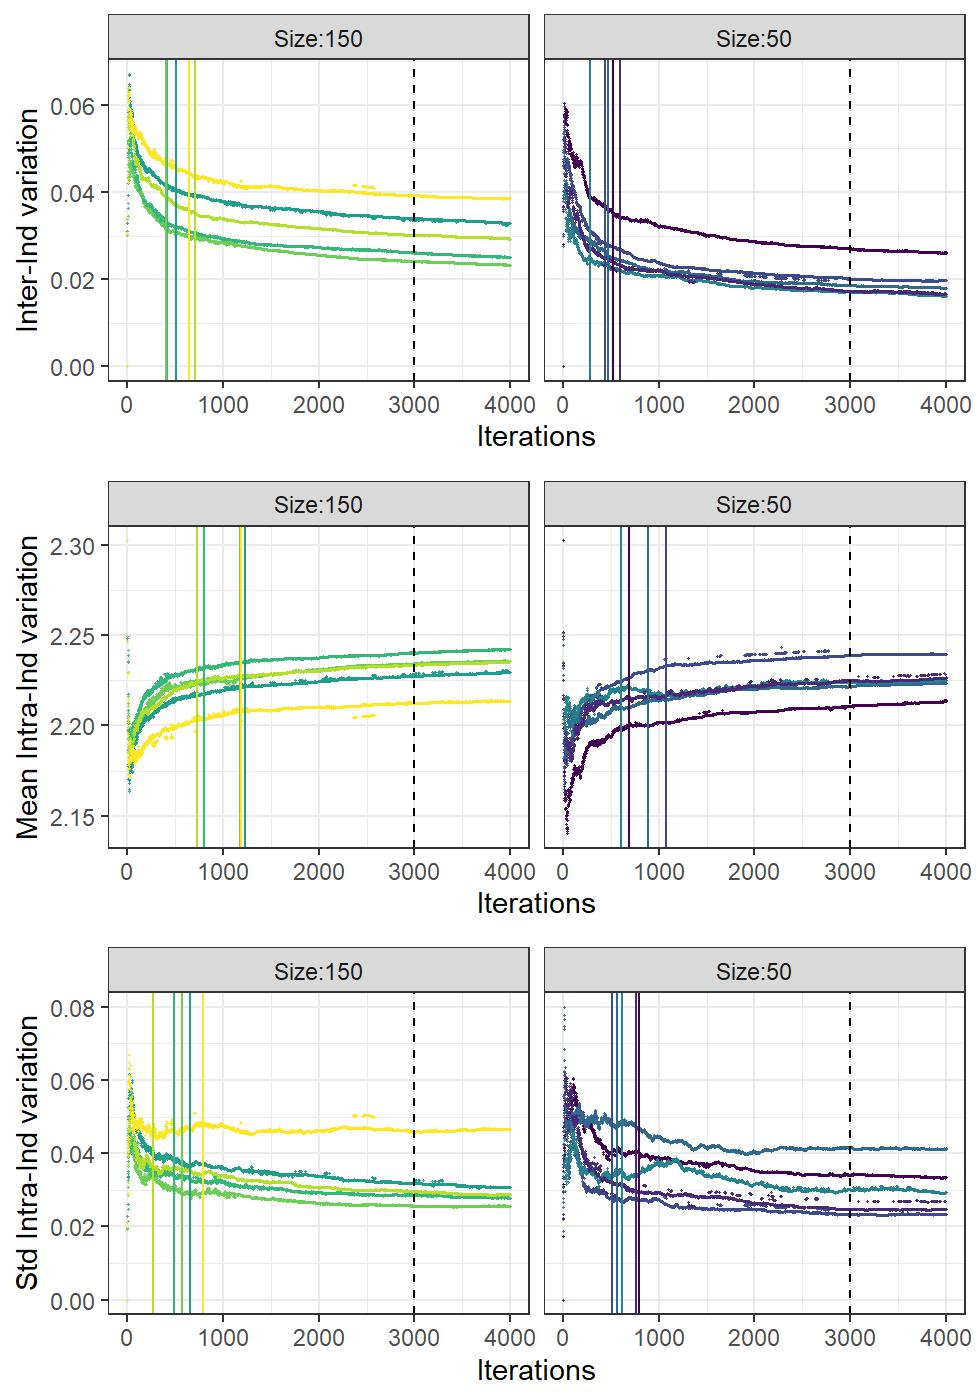
\includegraphics{./Figures/print timeline-1} 

}

\caption{Looking at the evolution of our different measures (top: inter-individual variability middle: mean of intra-individual variability bottom: std of intra-individual variability) with time. All agents speaks once in one interaction. We observe here 10 different simulations. Each simulation has a specific color. The plain vertical line shows the stabilization time for each replication (corresponding colors). The dashed black line shows our choice for selecting the final value of the language.}\label{fig:print timeline}
\end{figure}

According to this data, our measures of variation have always stabilized
after \emph{1500 interations.}

However, we decided here to study the language after agents have
interacted during \textbf{3000 iterations}. Indeed, it does not require
much more time to compute, and we make sure that the language will
indeed be stabilized in all our simulations.

\hypertarget{continuous}{%
\subsubsection{Continuous}\label{continuous}}

We did exactly the same but using continuous language simulations.

We observe the evolution of different measures: inter-individual
variation, the mean intra-individual variation and the std of
intra-individual variation.

We look here at 10 different simulations :

\begin{itemize}
\tightlist
\item
  5 simulations in networks with 50 agents
\item
  5 simulations in networks with 150 agents
\end{itemize}

In the following graph, each simulation is characterized by its color.

Please note that in the first graph below (inter-individual variation),
it seems that there is only one simulation (one color), but this is only
the case because all simulations have almost the same values, so the
points are superimposed.

\begin{figure}[!H]

{\centering 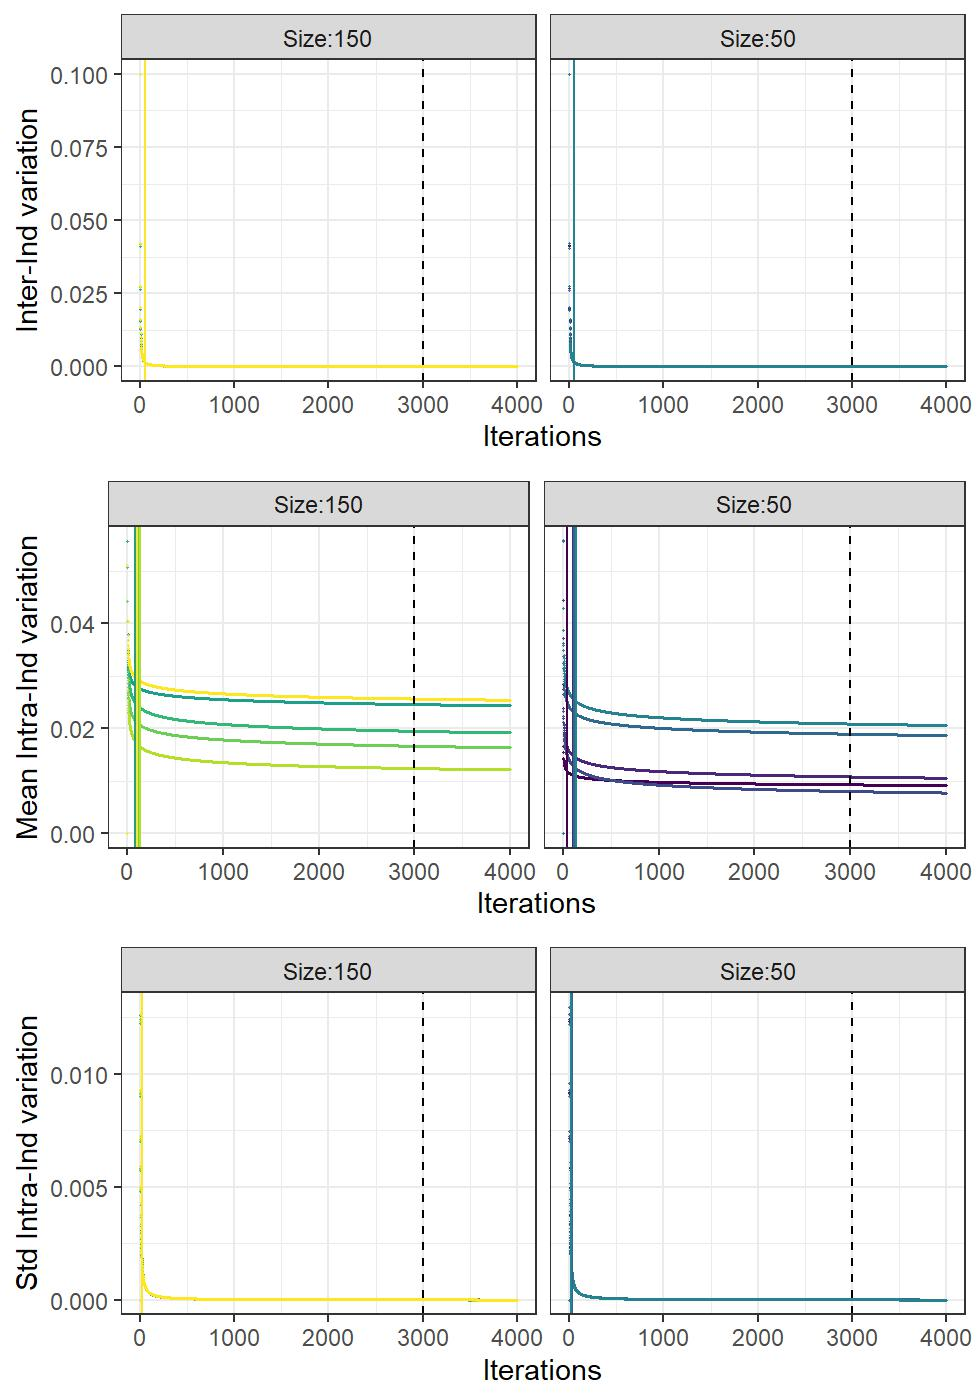
\includegraphics{./Figures/print timeline2-1} 

}

\caption{Looking at the evolution of our different measures (top: inter-individual variability middle: mean of intra-individual variability bottom: std of intra-individual variability) with time. All agents speaks once in one interaction. We observe here 10 different simulations. Each simulation has a specific color. The plain vertical line shows the stabilization time for each replication (corresponding colors). The dashed black line shows our choice for selecting the final value of the language.}\label{fig:print timeline2}
\end{figure}

Popualtions with continuous language take way less time to stabilize.
For simplicity reasons, we use the same threshold as for multinomial
language.

\textbf{Summary}:

We record the final value of the language after 3000 iterations.

\hypertarget{dataset-1-comparing-sets-of-networks}{%
\subsection{DATASET 1: comparing sets of
networks}\label{dataset-1-comparing-sets-of-networks}}

\hypertarget{multinomial-1}{%
\subsubsection{Multinomial}\label{multinomial-1}}

This part first presents the detailed results for each metric. However,
you can refer to the \protect\hyperlink{summary-multinomial}{Summary
multinomial} part, where you can see all the information in one plot.

\hypertarget{pathlength}{%
\paragraph{Pathlength}\label{pathlength}}

These sets of networks were obtained using \textbf{scale-free} networks.

We first observe the values of the two sets:

\begin{longtable}[]{@{}
  >{\raggedright\arraybackslash}p{(\columnwidth - 14\tabcolsep) * \real{0.2151}}
  >{\raggedleft\arraybackslash}p{(\columnwidth - 14\tabcolsep) * \real{0.1183}}
  >{\raggedleft\arraybackslash}p{(\columnwidth - 14\tabcolsep) * \real{0.1075}}
  >{\raggedleft\arraybackslash}p{(\columnwidth - 14\tabcolsep) * \real{0.1183}}
  >{\raggedleft\arraybackslash}p{(\columnwidth - 14\tabcolsep) * \real{0.1505}}
  >{\raggedleft\arraybackslash}p{(\columnwidth - 14\tabcolsep) * \real{0.0968}}
  >{\raggedleft\arraybackslash}p{(\columnwidth - 14\tabcolsep) * \real{0.0538}}
  >{\raggedright\arraybackslash}p{(\columnwidth - 14\tabcolsep) * \real{0.1398}}@{}}
\toprule()
\begin{minipage}[b]{\linewidth}\raggedright
\end{minipage} & \begin{minipage}[b]{\linewidth}\raggedleft
pathlength
\end{minipage} & \begin{minipage}[b]{\linewidth}\raggedleft
neighbors
\end{minipage} & \begin{minipage}[b]{\linewidth}\raggedleft
clustering
\end{minipage} & \begin{minipage}[b]{\linewidth}\raggedleft
assortativity
\end{minipage} & \begin{minipage}[b]{\linewidth}\raggedleft
exponent
\end{minipage} & \begin{minipage}[b]{\linewidth}\raggedleft
size
\end{minipage} & \begin{minipage}[b]{\linewidth}\raggedright
network\_type
\end{minipage} \\
\midrule()
\endhead
Low pathlength set & 3.374239 & 1.96 & 0 & -0.3125999 & 2.798979 & 50 &
Scalefree \\
High pathlength set & 4.987007 & 1.96 & 0 & -0.3057365 & 2.790429 & 50 &
Scalefree \\
\bottomrule()
\end{longtable}

This should be interpreted in the following way:

\begin{itemize}
\tightlist
\item
  there is a difference of 1.6128 between the two sets concerning
  \emph{pathlength}
\item
  there are differences of 0 for the \emph{neighbors}, 0 for the
  \emph{clustering} coefficient, 0.0069 for the \emph{assortativity},
  -0.0085 for the \emph{exponent}, and 0 for the \emph{size}
\end{itemize}

Thus, we compare the differences in inter and intra-individual variation
between the two sets. We believe that these differences will reflect the
differences in \emph{pathlength}, as the other metrics are kept (almost)
constant.

We look at the differences between the two sets:

\begin{figure}[!H]

{\centering 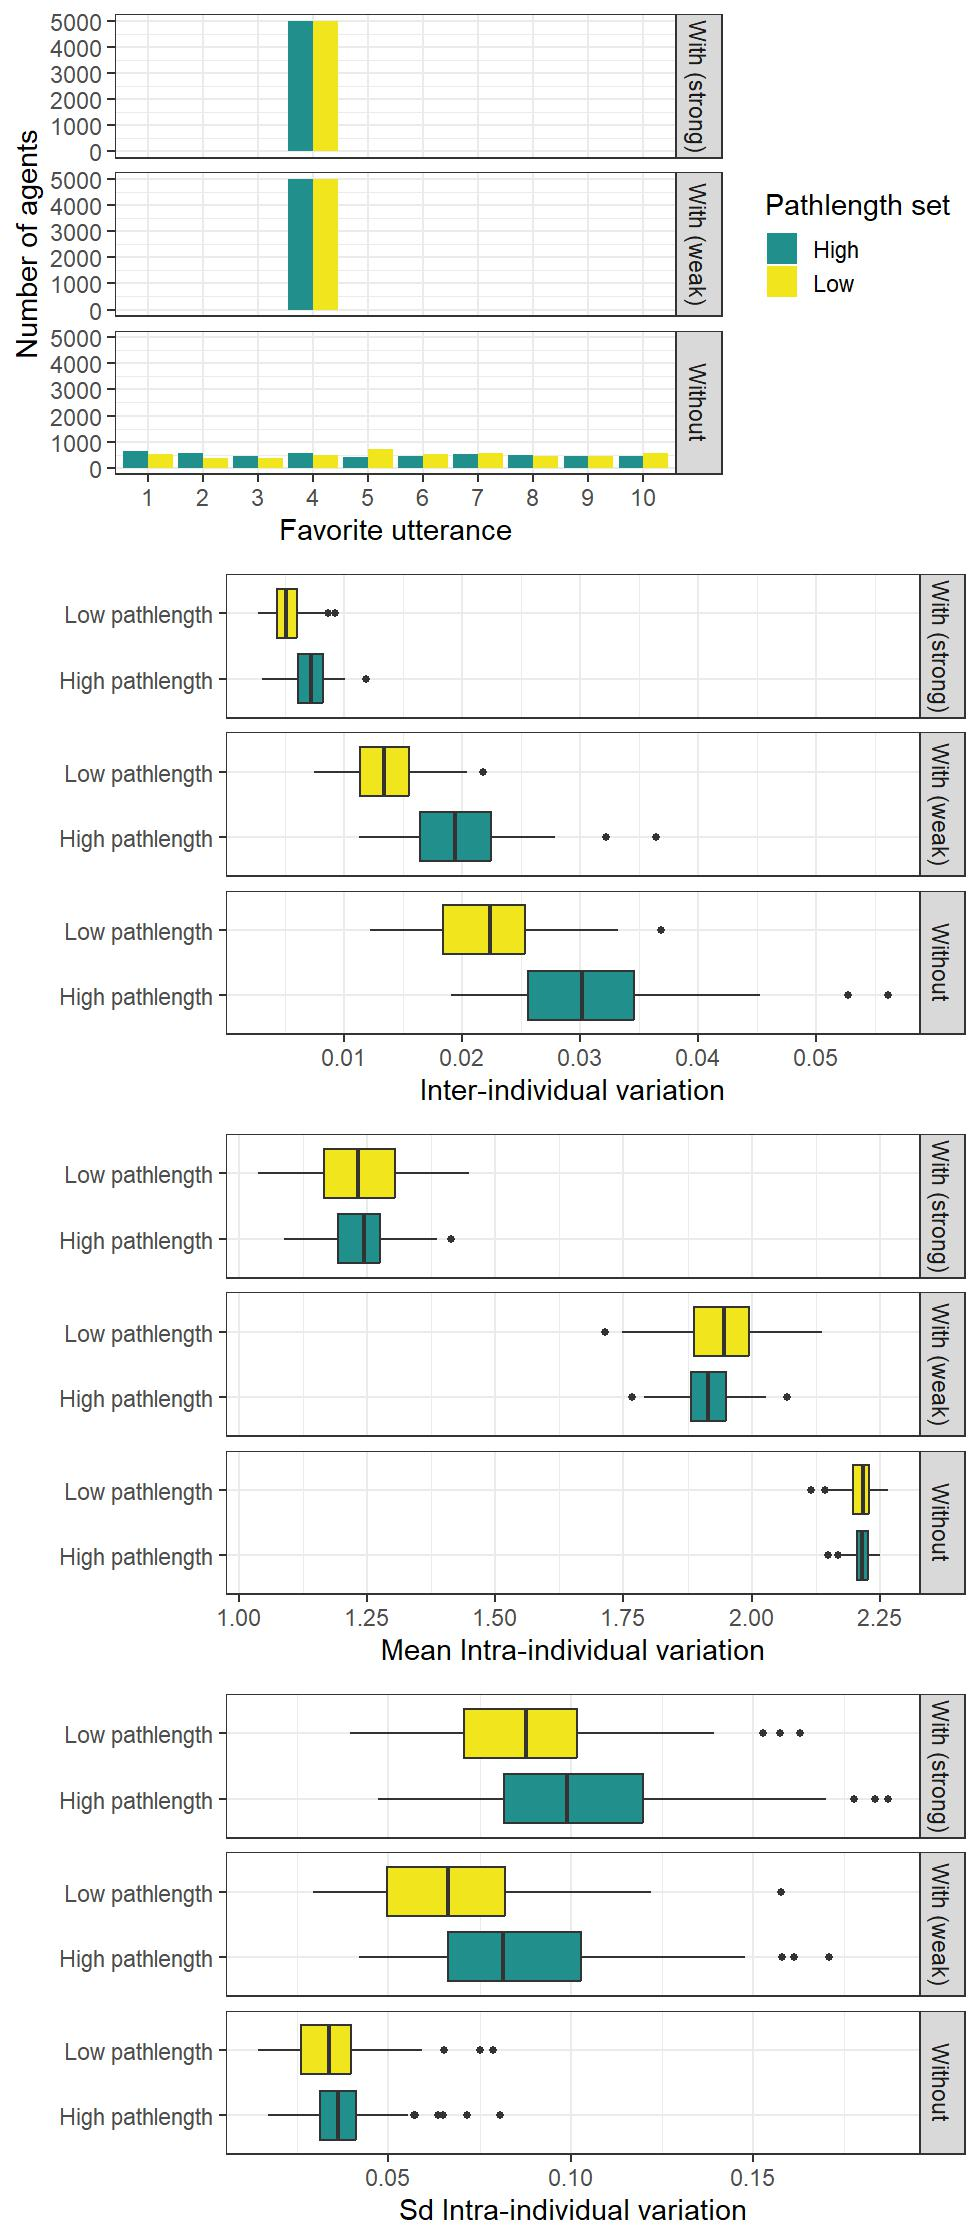
\includegraphics{./Figures/unnamed-chunk-6-1} 

}

\caption{Looking at the variability inter- and intra-individual in sets varying in *pathlength*. The first graph shows the value of the language: it shows the favorite utterance for each agents in the three types of population (variable initial language exposure). The second graph shows the  inter-individual variation (the x scale is the average Kullback-Leibler divergence on all pairs of agents). The third and fourth graph show respectively the mean and standard deviation on the intra-individual variation for all agents (the x scale shows respectively the mean and the std of the entropy on the Dirichlet internal representation of agents). In all the following graphs, green shows high value in the metrics while yellow shows low value in the metric.}\label{fig:unnamed-chunk-6}
\end{figure}

Here, we want to understand whether the effect size under these
differences is high or low.

We apply Cohen's d test and a classic t.test, in networks
\textbf{without} language exposure, \textbf{with (weak)} language
exposure, and \textbf{with (strong)} language exposure. We gathered the
results in a summary table:

Cohen's \emph{D}:

\begin{longtable}[]{@{}
  >{\raggedright\arraybackslash}p{(\columnwidth - 12\tabcolsep) * \real{0.1571}}
  >{\raggedright\arraybackslash}p{(\columnwidth - 12\tabcolsep) * \real{0.2000}}
  >{\raggedright\arraybackslash}p{(\columnwidth - 12\tabcolsep) * \real{0.2000}}
  >{\raggedleft\arraybackslash}p{(\columnwidth - 12\tabcolsep) * \real{0.1000}}
  >{\raggedleft\arraybackslash}p{(\columnwidth - 12\tabcolsep) * \real{0.1429}}
  >{\raggedleft\arraybackslash}p{(\columnwidth - 12\tabcolsep) * \real{0.1000}}
  >{\raggedleft\arraybackslash}p{(\columnwidth - 12\tabcolsep) * \real{0.1000}}@{}}
\toprule()
\begin{minipage}[b]{\linewidth}\raggedright
Measure
\end{minipage} & \begin{minipage}[b]{\linewidth}\raggedright
TypeVariation
\end{minipage} & \begin{minipage}[b]{\linewidth}\raggedright
TypeLangage
\end{minipage} & \begin{minipage}[b]{\linewidth}\raggedleft
CohenD
\end{minipage} & \begin{minipage}[b]{\linewidth}\raggedleft
Magnitude
\end{minipage} & \begin{minipage}[b]{\linewidth}\raggedleft
CI\_Inf
\end{minipage} & \begin{minipage}[b]{\linewidth}\raggedleft
CI\_Sup
\end{minipage} \\
\midrule()
\endhead
pathlength & Inter & Without & 1.464 & 4 & 1.150 & 1.778 \\
pathlength & Inter & With (weak) & 1.522 & 4 & 1.205 & 1.838 \\
pathlength & Inter & With (strong) & 1.247 & 4 & 0.942 & 1.552 \\
pathlength & Mean Intra & Without & 0.070 & 1 & -0.209 & 0.349 \\
pathlength & Mean Intra & With (weak) & 0.308 & 2 & 0.588 & 0.027 \\
pathlength & Mean Intra & With (strong) & 0.023 & 1 & -0.256 & 0.302 \\
pathlength & Std Intra & Without & 0.296 & 2 & 0.016 & 0.577 \\
pathlength & Std Intra & With (weak) & 0.677 & 3 & 0.390 & 0.964 \\
pathlength & Std Intra & With (strong) & 0.505 & 3 & 0.221 & 0.788 \\
\bottomrule()
\end{longtable}

\emph{T}-Test:

\begin{longtable}[]{@{}
  >{\raggedright\arraybackslash}p{(\columnwidth - 14\tabcolsep) * \real{0.1392}}
  >{\raggedright\arraybackslash}p{(\columnwidth - 14\tabcolsep) * \real{0.1772}}
  >{\raggedright\arraybackslash}p{(\columnwidth - 14\tabcolsep) * \real{0.1772}}
  >{\raggedleft\arraybackslash}p{(\columnwidth - 14\tabcolsep) * \real{0.1013}}
  >{\raggedleft\arraybackslash}p{(\columnwidth - 14\tabcolsep) * \real{0.1013}}
  >{\raggedleft\arraybackslash}p{(\columnwidth - 14\tabcolsep) * \real{0.1266}}
  >{\raggedleft\arraybackslash}p{(\columnwidth - 14\tabcolsep) * \real{0.0886}}
  >{\raggedleft\arraybackslash}p{(\columnwidth - 14\tabcolsep) * \real{0.0886}}@{}}
\toprule()
\begin{minipage}[b]{\linewidth}\raggedright
Measure
\end{minipage} & \begin{minipage}[b]{\linewidth}\raggedright
TypeVariation
\end{minipage} & \begin{minipage}[b]{\linewidth}\raggedright
TypeLangage
\end{minipage} & \begin{minipage}[b]{\linewidth}\raggedleft
T\_value
\end{minipage} & \begin{minipage}[b]{\linewidth}\raggedleft
DF
\end{minipage} & \begin{minipage}[b]{\linewidth}\raggedleft
PValue
\end{minipage} & \begin{minipage}[b]{\linewidth}\raggedleft
CI\_Inf
\end{minipage} & \begin{minipage}[b]{\linewidth}\raggedleft
CI\_Sup
\end{minipage} \\
\midrule()
\endhead
pathlength & Inter & Without & 10.351 & 185.325 & 0.0000000 & 1.150 &
1.778 \\
pathlength & Inter & With (weak) & 10.760 & 173.081 & 0.0000000 & 1.205
& 1.838 \\
pathlength & Inter & With (strong) & 8.819 & 194.129 & 0.0000000 & 0.942
& 1.552 \\
pathlength & Mean Intra & Without & 0.493 & 183.826 & 0.6226403 & -0.209
& 0.349 \\
pathlength & Mean Intra & With (weak) & -2.176 & 183.850 & 0.0308327 &
-0.588 & -0.027 \\
pathlength & Mean Intra & With (strong) & -0.163 & 177.904 & 0.8706430 &
-0.302 & 0.256 \\
pathlength & Std Intra & Without & 2.095 & 194.168 & 0.0374853 & 0.016 &
0.577 \\
pathlength & Std Intra & With (weak) & 4.789 & 196.574 & 0.0000033 &
0.390 & 0.964 \\
pathlength & Std Intra & With (strong) & 3.568 & 192.189 & 0.0004535 &
0.221 & 0.788 \\
\bottomrule()
\end{longtable}

\hypertarget{assortativity}{%
\paragraph{Assortativity}\label{assortativity}}

These sets of networks were obtained using \textbf{scale-free} networks.

We first observe the values of the two sets:

\begin{longtable}[]{@{}
  >{\raggedright\arraybackslash}p{(\columnwidth - 14\tabcolsep) * \real{0.2396}}
  >{\raggedleft\arraybackslash}p{(\columnwidth - 14\tabcolsep) * \real{0.1146}}
  >{\raggedleft\arraybackslash}p{(\columnwidth - 14\tabcolsep) * \real{0.1042}}
  >{\raggedleft\arraybackslash}p{(\columnwidth - 14\tabcolsep) * \real{0.1146}}
  >{\raggedleft\arraybackslash}p{(\columnwidth - 14\tabcolsep) * \real{0.1458}}
  >{\raggedleft\arraybackslash}p{(\columnwidth - 14\tabcolsep) * \real{0.0937}}
  >{\raggedleft\arraybackslash}p{(\columnwidth - 14\tabcolsep) * \real{0.0521}}
  >{\raggedright\arraybackslash}p{(\columnwidth - 14\tabcolsep) * \real{0.1354}}@{}}
\toprule()
\begin{minipage}[b]{\linewidth}\raggedright
\end{minipage} & \begin{minipage}[b]{\linewidth}\raggedleft
pathlength
\end{minipage} & \begin{minipage}[b]{\linewidth}\raggedleft
neighbors
\end{minipage} & \begin{minipage}[b]{\linewidth}\raggedleft
clustering
\end{minipage} & \begin{minipage}[b]{\linewidth}\raggedleft
assortativity
\end{minipage} & \begin{minipage}[b]{\linewidth}\raggedleft
exponent
\end{minipage} & \begin{minipage}[b]{\linewidth}\raggedleft
size
\end{minipage} & \begin{minipage}[b]{\linewidth}\raggedright
network\_type
\end{minipage} \\
\midrule()
\endhead
Low assortativity set & 4.007469 & 1.96 & 0 & -0.4832008 & 2.747048 & 50
& Scalefree \\
High assortativity set & 4.016071 & 1.96 & 0 & -0.1650383 & 2.752900 &
50 & Scalefree \\
\bottomrule()
\end{longtable}

This should be interpreted in the following way:

\begin{itemize}
\tightlist
\item
  there is a difference of 0.3182 between the two sets concerning
  \emph{assortativity}
\item
  there are differences of 0 for the \emph{neighbors}, 0 for the
  \emph{clustering} coefficient, 0.0086 for the \emph{pathlength},
  0.0059 for the \emph{exponent}, and 0 for the \emph{size}
\end{itemize}

Thus, we compare the differences in inter and intra-individual variation
between the two sets. We believe that these differences will reflect the
differences in \emph{assortativity}, as the other metrics are kept
(almost) constant.

We look at the differences between the two sets:

\begin{figure}[!H]

{\centering 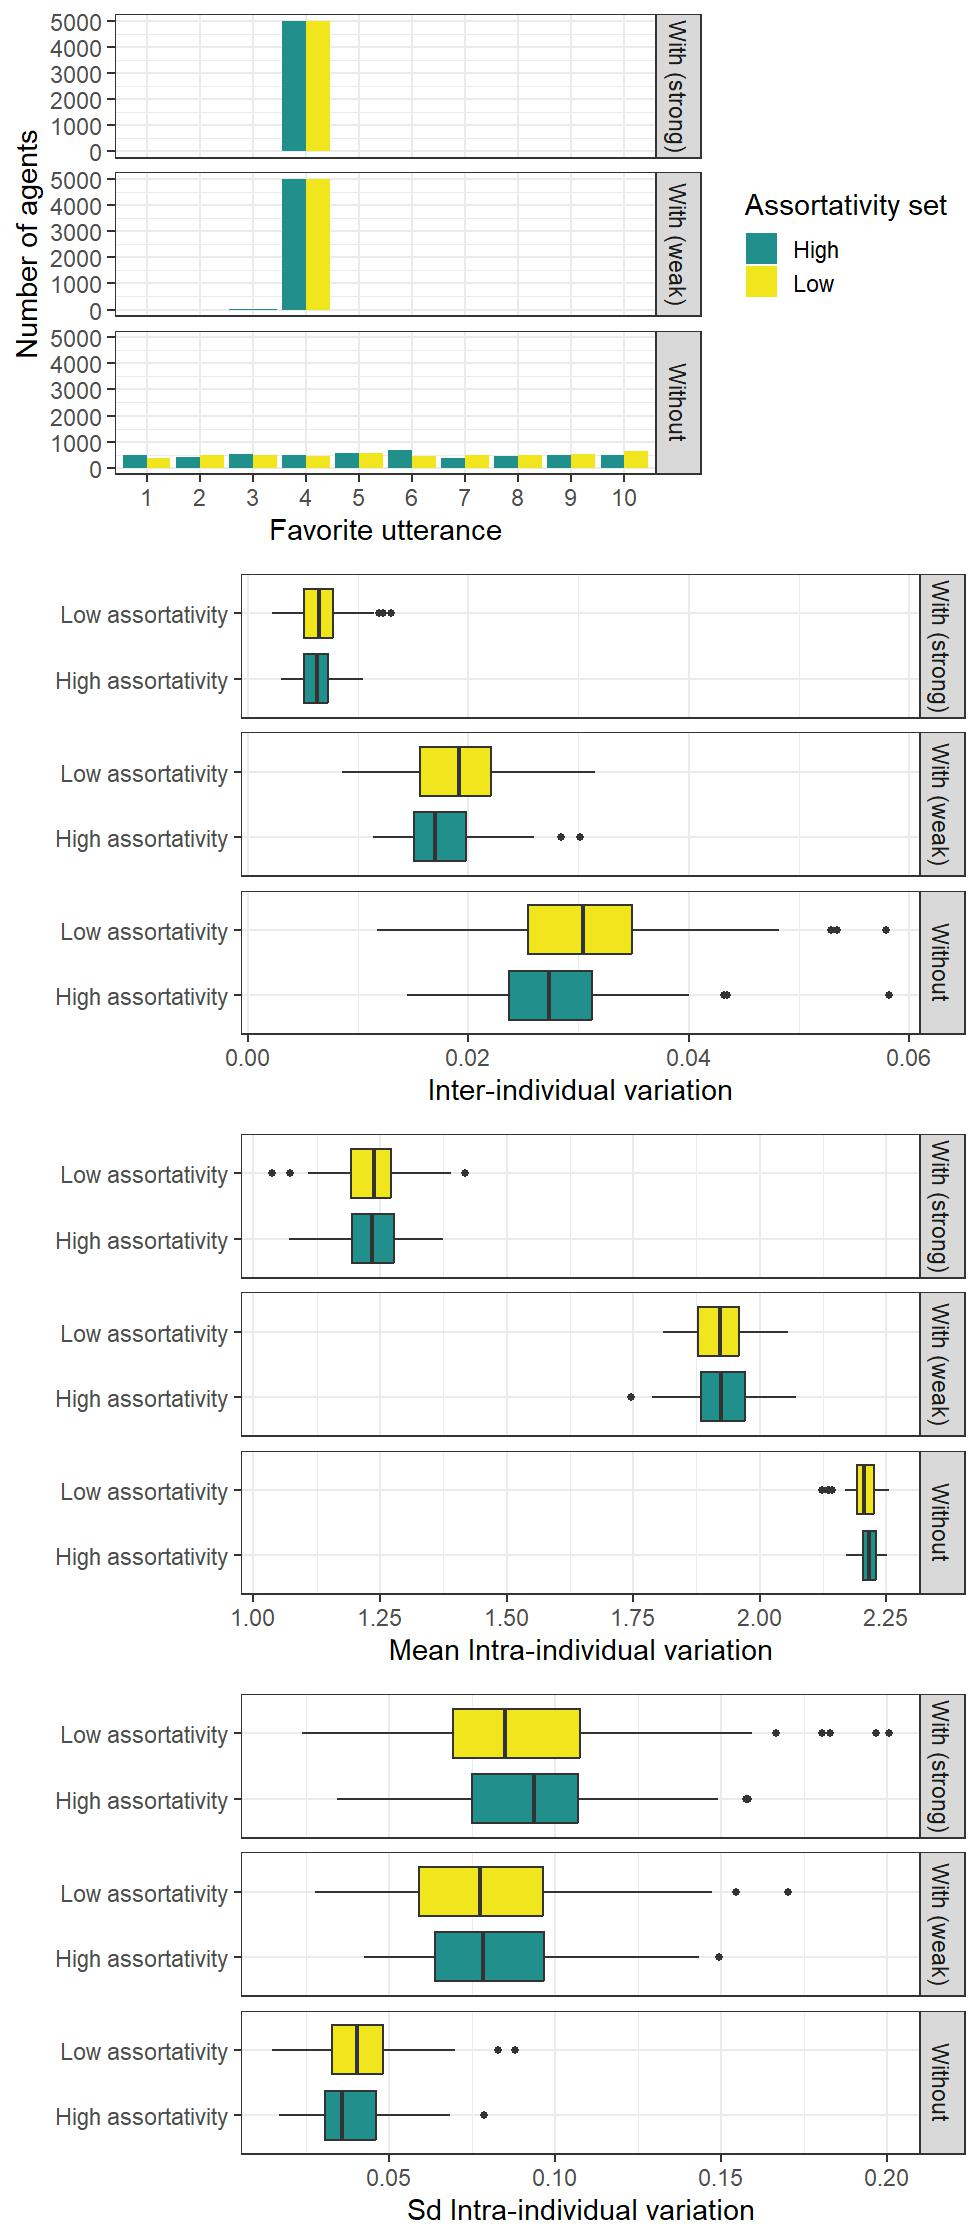
\includegraphics{./Figures/unnamed-chunk-10-1} 

}

\caption{Looking at the variability inter- and intra-individual in sets varying in *assortativity*. The first graph shows the value of the language: it shows the favorite utterance for each agents in the three types of population (variable initial language exposure). The second graph shows the  inter-individual variation (the x scale is the average Kullback-Leibler divergence on all pairs of agents). The third and fourth graph show respectively the mean and standard deviation on the intra-individual variation for all agents (the x scale shows respectively the mean and the std of the entropy on the Dirichlet internal representation of agents). In all the following graphs, green shows high value in the metrics while yellow shows low value in the metric.}\label{fig:unnamed-chunk-10}
\end{figure}

We want to understand whether the effect size under these differences is
high or low.

We apply Cohen's d test and a classic t.test, in networks
\textbf{without} language exposure, \textbf{with (weak)} language
exposure, and \textbf{with (strong)} language exposure. We gathered the
results in a summary table:

Cohen's \emph{D}:

\begin{longtable}[]{@{}
  >{\raggedright\arraybackslash}p{(\columnwidth - 12\tabcolsep) * \real{0.1918}}
  >{\raggedright\arraybackslash}p{(\columnwidth - 12\tabcolsep) * \real{0.1918}}
  >{\raggedright\arraybackslash}p{(\columnwidth - 12\tabcolsep) * \real{0.1918}}
  >{\raggedleft\arraybackslash}p{(\columnwidth - 12\tabcolsep) * \real{0.0959}}
  >{\raggedleft\arraybackslash}p{(\columnwidth - 12\tabcolsep) * \real{0.1370}}
  >{\raggedleft\arraybackslash}p{(\columnwidth - 12\tabcolsep) * \real{0.0959}}
  >{\raggedleft\arraybackslash}p{(\columnwidth - 12\tabcolsep) * \real{0.0959}}@{}}
\toprule()
\begin{minipage}[b]{\linewidth}\raggedright
Measure
\end{minipage} & \begin{minipage}[b]{\linewidth}\raggedright
TypeVariation
\end{minipage} & \begin{minipage}[b]{\linewidth}\raggedright
TypeLangage
\end{minipage} & \begin{minipage}[b]{\linewidth}\raggedleft
CohenD
\end{minipage} & \begin{minipage}[b]{\linewidth}\raggedleft
Magnitude
\end{minipage} & \begin{minipage}[b]{\linewidth}\raggedleft
CI\_Inf
\end{minipage} & \begin{minipage}[b]{\linewidth}\raggedleft
CI\_Sup
\end{minipage} \\
\midrule()
\endhead
assortativity & Inter & Without & 0.405 & 2 & 0.686 & 0.123 \\
assortativity & Inter & With (weak) & 0.392 & 2 & 0.673 & 0.110 \\
assortativity & Inter & With (strong) & 0.140 & 1 & -0.139 & 0.419 \\
assortativity & Mean Intra & Without & 0.467 & 2 & 0.184 & 0.750 \\
assortativity & Mean Intra & With (weak) & 0.083 & 1 & -0.196 & 0.362 \\
assortativity & Mean Intra & With (strong) & 0.023 & 1 & -0.256 &
0.302 \\
assortativity & Std Intra & Without & 0.234 & 2 & -0.046 & 0.514 \\
assortativity & Std Intra & With (weak) & 0.050 & 1 & -0.229 & 0.329 \\
assortativity & Std Intra & With (strong) & 0.034 & 1 & -0.245 &
0.313 \\
\bottomrule()
\end{longtable}

\emph{T}-Test:

\begin{longtable}[]{@{}
  >{\raggedright\arraybackslash}p{(\columnwidth - 14\tabcolsep) * \real{0.1707}}
  >{\raggedright\arraybackslash}p{(\columnwidth - 14\tabcolsep) * \real{0.1707}}
  >{\raggedright\arraybackslash}p{(\columnwidth - 14\tabcolsep) * \real{0.1707}}
  >{\raggedleft\arraybackslash}p{(\columnwidth - 14\tabcolsep) * \real{0.0976}}
  >{\raggedleft\arraybackslash}p{(\columnwidth - 14\tabcolsep) * \real{0.0976}}
  >{\raggedleft\arraybackslash}p{(\columnwidth - 14\tabcolsep) * \real{0.1220}}
  >{\raggedleft\arraybackslash}p{(\columnwidth - 14\tabcolsep) * \real{0.0854}}
  >{\raggedleft\arraybackslash}p{(\columnwidth - 14\tabcolsep) * \real{0.0854}}@{}}
\toprule()
\begin{minipage}[b]{\linewidth}\raggedright
Measure
\end{minipage} & \begin{minipage}[b]{\linewidth}\raggedright
TypeVariation
\end{minipage} & \begin{minipage}[b]{\linewidth}\raggedright
TypeLangage
\end{minipage} & \begin{minipage}[b]{\linewidth}\raggedleft
T\_value
\end{minipage} & \begin{minipage}[b]{\linewidth}\raggedleft
DF
\end{minipage} & \begin{minipage}[b]{\linewidth}\raggedleft
PValue
\end{minipage} & \begin{minipage}[b]{\linewidth}\raggedleft
CI\_Inf
\end{minipage} & \begin{minipage}[b]{\linewidth}\raggedleft
CI\_Sup
\end{minipage} \\
\midrule()
\endhead
assortativity & Inter & Without & -2.861 & 187.026 & 0.0047091 & -0.686
& -0.123 \\
assortativity & Inter & With (weak) & -2.771 & 192.766 & 0.0061313 &
-0.673 & -0.110 \\
assortativity & Inter & With (strong) & -0.988 & 181.943 & 0.3244111 &
-0.419 & 0.139 \\
assortativity & Mean Intra & Without & 3.303 & 174.885 & 0.0011619 &
0.184 & 0.750 \\
assortativity & Mean Intra & With (weak) & 0.587 & 196.558 & 0.5580783 &
-0.196 & 0.362 \\
assortativity & Mean Intra & With (strong) & -0.165 & 194.361 &
0.8694981 & -0.302 & 0.256 \\
assortativity & Std Intra & Without & -1.655 & 192.451 & 0.0996226 &
-0.514 & 0.046 \\
assortativity & Std Intra & With (weak) & 0.355 & 188.545 & 0.7227121 &
-0.229 & 0.329 \\
assortativity & Std Intra & With (strong) & 0.242 & 175.069 & 0.8089962
& -0.245 & 0.313 \\
\bottomrule()
\end{longtable}

\hypertarget{exponent}{%
\paragraph{Exponent}\label{exponent}}

These sets of networks were obtained using \textbf{scale-free} networks.

We first observe the values of the two sets:

\begin{longtable}[]{@{}
  >{\raggedright\arraybackslash}p{(\columnwidth - 14\tabcolsep) * \real{0.1978}}
  >{\raggedleft\arraybackslash}p{(\columnwidth - 14\tabcolsep) * \real{0.1209}}
  >{\raggedleft\arraybackslash}p{(\columnwidth - 14\tabcolsep) * \real{0.1099}}
  >{\raggedleft\arraybackslash}p{(\columnwidth - 14\tabcolsep) * \real{0.1209}}
  >{\raggedleft\arraybackslash}p{(\columnwidth - 14\tabcolsep) * \real{0.1538}}
  >{\raggedleft\arraybackslash}p{(\columnwidth - 14\tabcolsep) * \real{0.0989}}
  >{\raggedleft\arraybackslash}p{(\columnwidth - 14\tabcolsep) * \real{0.0549}}
  >{\raggedright\arraybackslash}p{(\columnwidth - 14\tabcolsep) * \real{0.1429}}@{}}
\toprule()
\begin{minipage}[b]{\linewidth}\raggedright
\end{minipage} & \begin{minipage}[b]{\linewidth}\raggedleft
pathlength
\end{minipage} & \begin{minipage}[b]{\linewidth}\raggedleft
neighbors
\end{minipage} & \begin{minipage}[b]{\linewidth}\raggedleft
clustering
\end{minipage} & \begin{minipage}[b]{\linewidth}\raggedleft
assortativity
\end{minipage} & \begin{minipage}[b]{\linewidth}\raggedleft
exponent
\end{minipage} & \begin{minipage}[b]{\linewidth}\raggedleft
size
\end{minipage} & \begin{minipage}[b]{\linewidth}\raggedright
network\_type
\end{minipage} \\
\midrule()
\endhead
Low exponent set & 4.101233 & 1.96 & 0 & -0.3545311 & 2.552332 & 50 &
Scalefree \\
High exponent set & 4.093472 & 1.96 & 0 & -0.3459061 & 3.037600 & 50 &
Scalefree \\
\bottomrule()
\end{longtable}

This should be interpreted in the following way:

\begin{itemize}
\tightlist
\item
  there is a difference of 0.4853 between the two sets concerning
  \emph{exponent}
\item
  there are differences of 0 for the \emph{neighbors}, 0 for the
  \emph{clustering} coefficient, -0.0078 for the \emph{pathlength},
  0.0086 for the \emph{assortativity}, and 0 for the \emph{size}
\end{itemize}

Thus, we compare the differences in inter and intra-individual variation
between the two sets. We believe that these differences will reflect the
differences in exponent, as the other metrics are kept (almost)
constant.

We look at the differences between the two sets:

\begin{figure}[!H]

{\centering 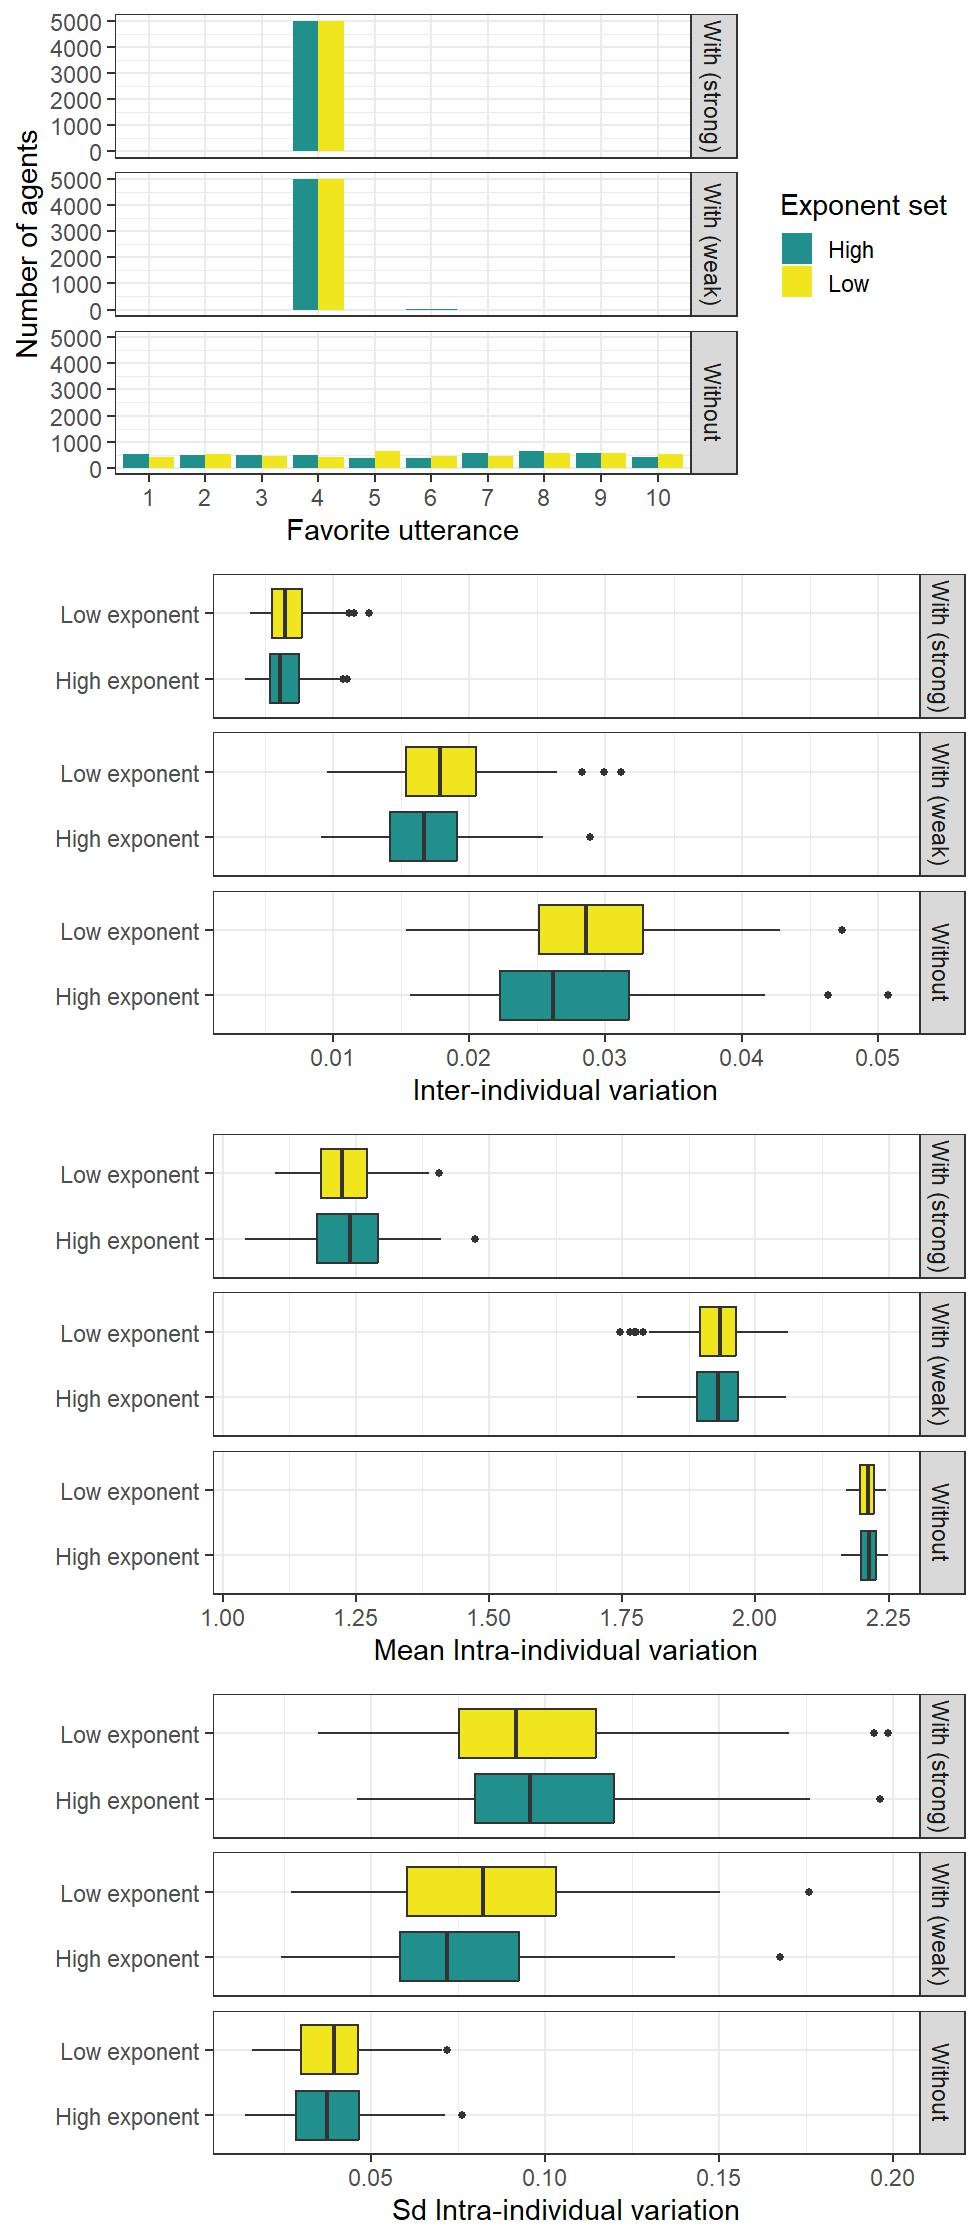
\includegraphics{./Figures/unnamed-chunk-14-1} 

}

\caption{Looking at the variability inter- and intra-individual in sets varying in *exponent*. The first graph shows the value of the language: it shows the favorite utterance for each agents in the three types of population (variable initial language exposure). The second graph shows the  inter-individual variation (the x scale is the average Kullback-Leibler divergence on all pairs of agents). The third and fourth graph show respectively the mean and standard deviation on the intra-individual variation for all agents (the x scale shows respectively the mean and the std of the entropy on the Dirichlet internal representation of agents). In all the following graphs, green shows high value in the metrics while yellow shows low value in the metric.}\label{fig:unnamed-chunk-14}
\end{figure}

Here, we want to understand whether the effect size under these
differences is high or low.

We apply Cohen's d test and a classic t.test, in networks
\textbf{without} language exposure, \textbf{with (weak)} language
exposure, and \textbf{with (strong)} language exposure. We gathered the
results in a summary table:

Cohen's \emph{D}:

\begin{longtable}[]{@{}
  >{\raggedright\arraybackslash}p{(\columnwidth - 12\tabcolsep) * \real{0.1324}}
  >{\raggedright\arraybackslash}p{(\columnwidth - 12\tabcolsep) * \real{0.2059}}
  >{\raggedright\arraybackslash}p{(\columnwidth - 12\tabcolsep) * \real{0.2059}}
  >{\raggedleft\arraybackslash}p{(\columnwidth - 12\tabcolsep) * \real{0.1029}}
  >{\raggedleft\arraybackslash}p{(\columnwidth - 12\tabcolsep) * \real{0.1471}}
  >{\raggedleft\arraybackslash}p{(\columnwidth - 12\tabcolsep) * \real{0.1029}}
  >{\raggedleft\arraybackslash}p{(\columnwidth - 12\tabcolsep) * \real{0.1029}}@{}}
\toprule()
\begin{minipage}[b]{\linewidth}\raggedright
Measure
\end{minipage} & \begin{minipage}[b]{\linewidth}\raggedright
TypeVariation
\end{minipage} & \begin{minipage}[b]{\linewidth}\raggedright
TypeLangage
\end{minipage} & \begin{minipage}[b]{\linewidth}\raggedleft
CohenD
\end{minipage} & \begin{minipage}[b]{\linewidth}\raggedleft
Magnitude
\end{minipage} & \begin{minipage}[b]{\linewidth}\raggedleft
CI\_Inf
\end{minipage} & \begin{minipage}[b]{\linewidth}\raggedleft
CI\_Sup
\end{minipage} \\
\midrule()
\endhead
exponent & Inter & Without & 0.313 & 2 & 0.593 & 0.032 \\
exponent & Inter & With (weak) & 0.330 & 2 & 0.611 & 0.049 \\
exponent & Inter & With (strong) & 0.152 & 1 & -0.128 & 0.431 \\
exponent & Mean Intra & Without & 0.081 & 1 & -0.198 & 0.360 \\
exponent & Mean Intra & With (weak) & 0.026 & 1 & -0.252 & 0.305 \\
exponent & Mean Intra & With (strong) & 0.076 & 1 & -0.203 & 0.355 \\
exponent & Std Intra & Without & 0.040 & 1 & -0.239 & 0.319 \\
exponent & Std Intra & With (weak) & 0.316 & 2 & 0.597 & 0.035 \\
exponent & Std Intra & With (strong) & 0.120 & 1 & -0.159 & 0.399 \\
\bottomrule()
\end{longtable}

\emph{T}-Test:

\begin{longtable}[]{@{}
  >{\raggedright\arraybackslash}p{(\columnwidth - 14\tabcolsep) * \real{0.1169}}
  >{\raggedright\arraybackslash}p{(\columnwidth - 14\tabcolsep) * \real{0.1818}}
  >{\raggedright\arraybackslash}p{(\columnwidth - 14\tabcolsep) * \real{0.1818}}
  >{\raggedleft\arraybackslash}p{(\columnwidth - 14\tabcolsep) * \real{0.1039}}
  >{\raggedleft\arraybackslash}p{(\columnwidth - 14\tabcolsep) * \real{0.1039}}
  >{\raggedleft\arraybackslash}p{(\columnwidth - 14\tabcolsep) * \real{0.1299}}
  >{\raggedleft\arraybackslash}p{(\columnwidth - 14\tabcolsep) * \real{0.0909}}
  >{\raggedleft\arraybackslash}p{(\columnwidth - 14\tabcolsep) * \real{0.0909}}@{}}
\toprule()
\begin{minipage}[b]{\linewidth}\raggedright
Measure
\end{minipage} & \begin{minipage}[b]{\linewidth}\raggedright
TypeVariation
\end{minipage} & \begin{minipage}[b]{\linewidth}\raggedright
TypeLangage
\end{minipage} & \begin{minipage}[b]{\linewidth}\raggedleft
T\_value
\end{minipage} & \begin{minipage}[b]{\linewidth}\raggedleft
DF
\end{minipage} & \begin{minipage}[b]{\linewidth}\raggedleft
PValue
\end{minipage} & \begin{minipage}[b]{\linewidth}\raggedleft
CI\_Inf
\end{minipage} & \begin{minipage}[b]{\linewidth}\raggedleft
CI\_Sup
\end{minipage} \\
\midrule()
\endhead
exponent & Inter & Without & -2.212 & 191.145 & 0.0281752 & -0.593 &
-0.032 \\
exponent & Inter & With (weak) & -2.332 & 195.703 & 0.0206957 & -0.611 &
-0.049 \\
exponent & Inter & With (strong) & -1.077 & 197.651 & 0.2827301 & -0.432
& 0.127 \\
exponent & Mean Intra & Without & 0.571 & 197.918 & 0.5688533 & -0.198 &
0.360 \\
exponent & Mean Intra & With (weak) & -0.181 & 197.846 & 0.8569108 &
-0.304 & 0.253 \\
exponent & Mean Intra & With (strong) & 0.537 & 190.474 & 0.5920046 &
-0.203 & 0.355 \\
exponent & Std Intra & Without & -0.285 & 196.407 & 0.7757957 & -0.319 &
0.239 \\
exponent & Std Intra & With (weak) & -2.235 & 196.847 & 0.0265320 &
-0.597 & -0.035 \\
exponent & Std Intra & With (strong) & 0.846 & 197.731 & 0.3984539 &
-0.159 & 0.399 \\
\bottomrule()
\end{longtable}

\hypertarget{size}{%
\paragraph{Size}\label{size}}

These sets of networks were obtained using \textbf{scale-free} networks.

We first observe the values of the two sets:

\begin{longtable}[]{@{}
  >{\raggedright\arraybackslash}p{(\columnwidth - 14\tabcolsep) * \real{0.1609}}
  >{\raggedleft\arraybackslash}p{(\columnwidth - 14\tabcolsep) * \real{0.1264}}
  >{\raggedleft\arraybackslash}p{(\columnwidth - 14\tabcolsep) * \real{0.1149}}
  >{\raggedleft\arraybackslash}p{(\columnwidth - 14\tabcolsep) * \real{0.1264}}
  >{\raggedleft\arraybackslash}p{(\columnwidth - 14\tabcolsep) * \real{0.1609}}
  >{\raggedleft\arraybackslash}p{(\columnwidth - 14\tabcolsep) * \real{0.1034}}
  >{\raggedleft\arraybackslash}p{(\columnwidth - 14\tabcolsep) * \real{0.0575}}
  >{\raggedright\arraybackslash}p{(\columnwidth - 14\tabcolsep) * \real{0.1494}}@{}}
\toprule()
\begin{minipage}[b]{\linewidth}\raggedright
\end{minipage} & \begin{minipage}[b]{\linewidth}\raggedleft
pathlength
\end{minipage} & \begin{minipage}[b]{\linewidth}\raggedleft
neighbors
\end{minipage} & \begin{minipage}[b]{\linewidth}\raggedleft
clustering
\end{minipage} & \begin{minipage}[b]{\linewidth}\raggedleft
assortativity
\end{minipage} & \begin{minipage}[b]{\linewidth}\raggedleft
exponent
\end{minipage} & \begin{minipage}[b]{\linewidth}\raggedleft
size
\end{minipage} & \begin{minipage}[b]{\linewidth}\raggedright
network\_type
\end{minipage} \\
\midrule()
\endhead
Low size set & 4.490076 & 1.96 & 0 & -0.2974416 & 2.848549 & 50 &
Scalefree \\
High size set & 4.499676 & 1.98 & 0 & -0.2908039 & 2.851606 & 100 &
Scalefree \\
\bottomrule()
\end{longtable}

This should be interpreted in the following way:

\begin{itemize}
\tightlist
\item
  there is a difference of 50 between the two sets concerning
  \emph{size}
\item
  there are differences of 0.02 for the \emph{neighbors}, 0 for the
  \emph{clustering} coefficient, 0.0096 for the \emph{pathlength},
  0.0066 for the \emph{assortativity}, and 0.0031 for the
  \emph{exponent}
\end{itemize}

Thus, we compare the differences in inter and intra-individual variation
between the two sets. We believe that these differences will reflect the
differences in \emph{size}, as the other metrics are kept (almost)
constant.

We look at the differences between the two sets:

\begin{figure}[!H]

{\centering 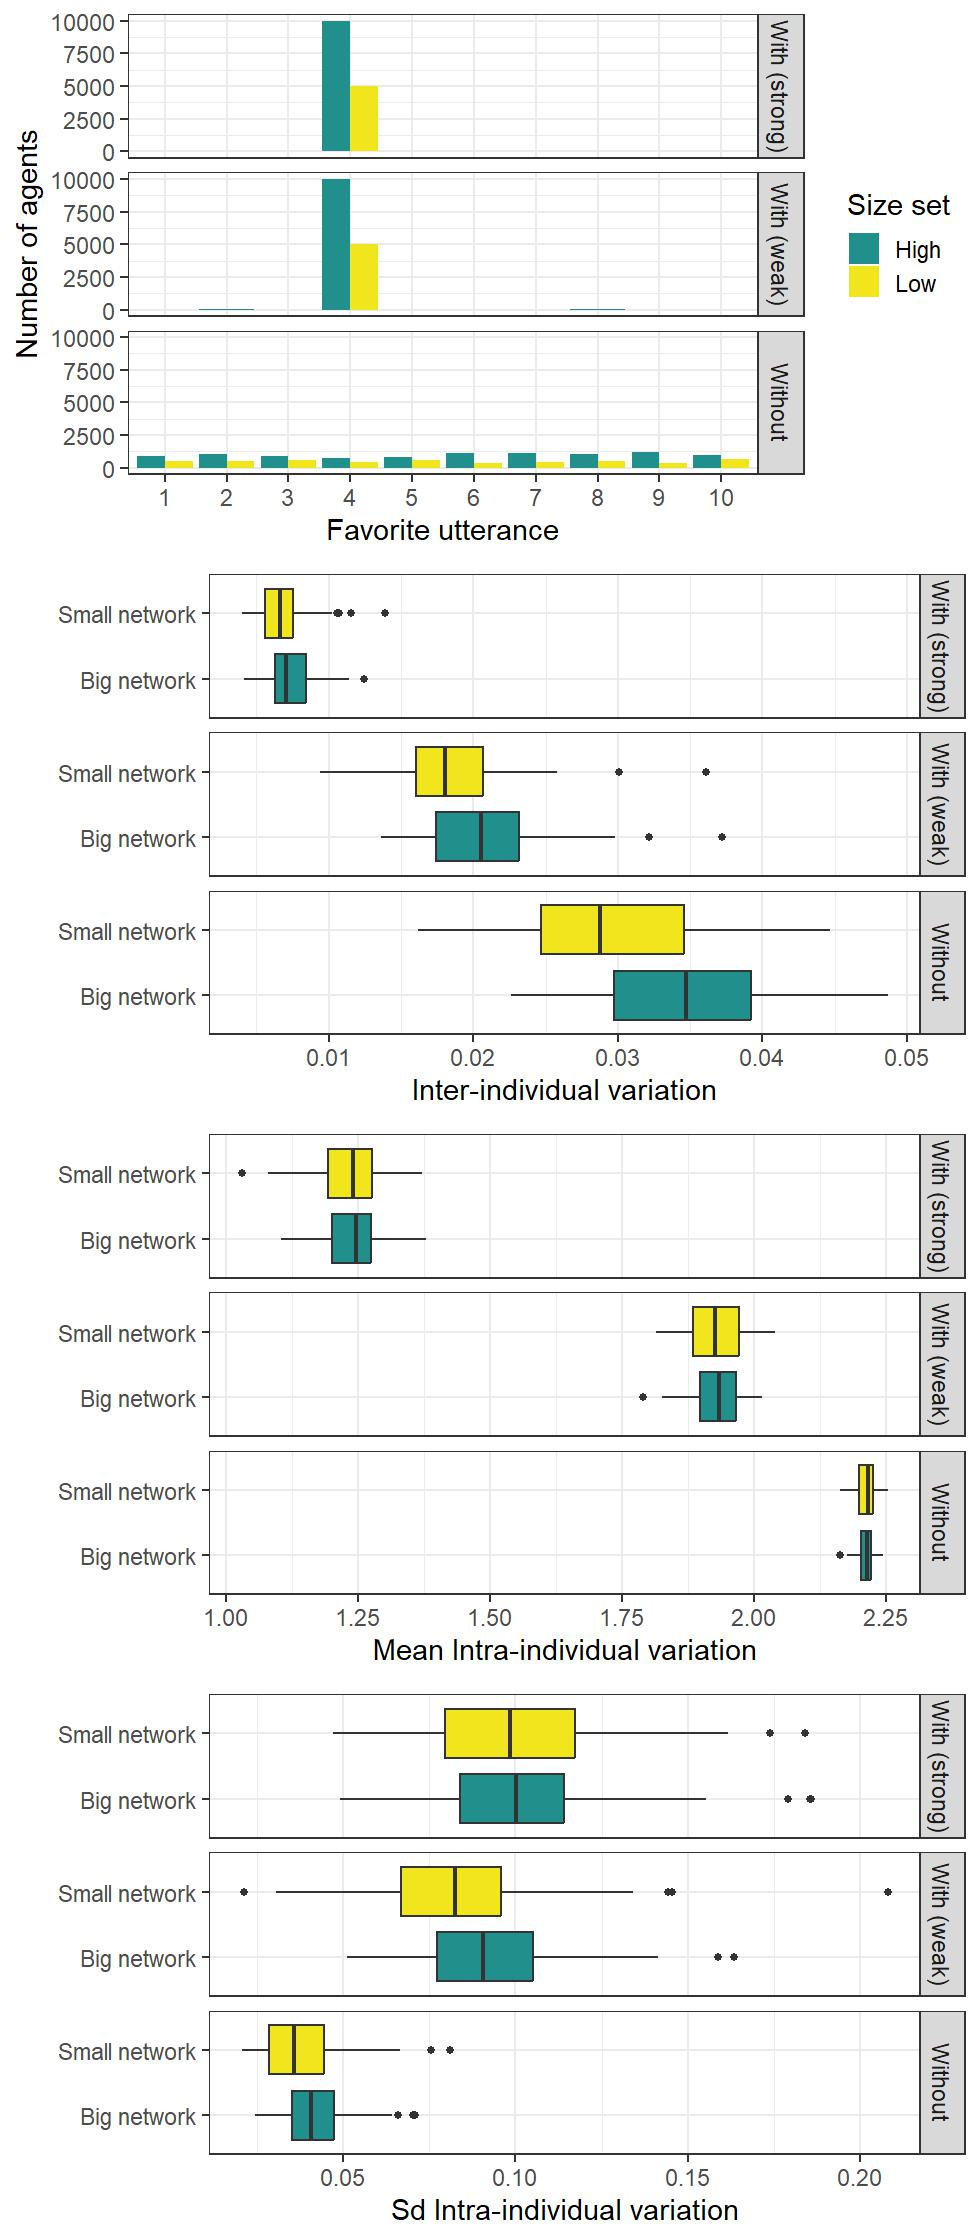
\includegraphics{./Figures/unnamed-chunk-18-1} 

}

\caption{Looking at the variability inter- and intra-individual in sets varying in *size*. The first graph shows the value of the language: it shows the favorite utterance for each agents in the three types of population (variable initial language exposure). The second graph shows the  inter-individual variation (the x scale is the average Kullback-Leibler divergence on all pairs of agents). The third and fourth graph show respectively the mean and standard deviation on the intra-individual variation for all agents (the x scale shows respectively the mean and the std of the entropy on the Dirichlet internal representation of agents). In all the following graphs, green shows high value in the metrics while yellow shows low value in the metric.}\label{fig:unnamed-chunk-18}
\end{figure}

Here, we want to understand whether the effect size under these
differences is high or low.

We apply Cohen's d test and a classic t.test, in networks
\textbf{without} language exposure, \textbf{with (weak)} language
exposure, and \textbf{with (strong)} language exposure. We gathered the
results in a summary table:

Cohen's \emph{D}:

\begin{longtable}[]{@{}
  >{\raggedright\arraybackslash}p{(\columnwidth - 12\tabcolsep) * \real{0.1194}}
  >{\raggedright\arraybackslash}p{(\columnwidth - 12\tabcolsep) * \real{0.2090}}
  >{\raggedright\arraybackslash}p{(\columnwidth - 12\tabcolsep) * \real{0.2090}}
  >{\raggedleft\arraybackslash}p{(\columnwidth - 12\tabcolsep) * \real{0.1045}}
  >{\raggedleft\arraybackslash}p{(\columnwidth - 12\tabcolsep) * \real{0.1493}}
  >{\raggedleft\arraybackslash}p{(\columnwidth - 12\tabcolsep) * \real{0.1045}}
  >{\raggedleft\arraybackslash}p{(\columnwidth - 12\tabcolsep) * \real{0.1045}}@{}}
\toprule()
\begin{minipage}[b]{\linewidth}\raggedright
Measure
\end{minipage} & \begin{minipage}[b]{\linewidth}\raggedright
TypeVariation
\end{minipage} & \begin{minipage}[b]{\linewidth}\raggedright
TypeLangage
\end{minipage} & \begin{minipage}[b]{\linewidth}\raggedleft
CohenD
\end{minipage} & \begin{minipage}[b]{\linewidth}\raggedleft
Magnitude
\end{minipage} & \begin{minipage}[b]{\linewidth}\raggedleft
CI\_Inf
\end{minipage} & \begin{minipage}[b]{\linewidth}\raggedleft
CI\_Sup
\end{minipage} \\
\midrule()
\endhead
size & Inter & Without & 0.894 & 4 & 0.601 & 1.186 \\
size & Inter & With (weak) & 0.492 & 2 & 0.209 & 0.775 \\
size & Inter & With (strong) & 0.304 & 2 & 0.024 & 0.585 \\
size & Mean Intra & Without & 0.112 & 1 & -0.167 & 0.391 \\
size & Mean Intra & With (weak) & 0.040 & 1 & -0.238 & 0.319 \\
size & Mean Intra & With (strong) & 0.104 & 1 & -0.175 & 0.383 \\
size & Std Intra & Without & 0.381 & 2 & 0.100 & 0.663 \\
size & Std Intra & With (weak) & 0.340 & 2 & 0.059 & 0.621 \\
size & Std Intra & With (strong) & 0.042 & 1 & -0.237 & 0.321 \\
\bottomrule()
\end{longtable}

\emph{T}-Test:

\begin{longtable}[]{@{}
  >{\raggedright\arraybackslash}p{(\columnwidth - 14\tabcolsep) * \real{0.1053}}
  >{\raggedright\arraybackslash}p{(\columnwidth - 14\tabcolsep) * \real{0.1842}}
  >{\raggedright\arraybackslash}p{(\columnwidth - 14\tabcolsep) * \real{0.1842}}
  >{\raggedleft\arraybackslash}p{(\columnwidth - 14\tabcolsep) * \real{0.1053}}
  >{\raggedleft\arraybackslash}p{(\columnwidth - 14\tabcolsep) * \real{0.1053}}
  >{\raggedleft\arraybackslash}p{(\columnwidth - 14\tabcolsep) * \real{0.1316}}
  >{\raggedleft\arraybackslash}p{(\columnwidth - 14\tabcolsep) * \real{0.0921}}
  >{\raggedleft\arraybackslash}p{(\columnwidth - 14\tabcolsep) * \real{0.0921}}@{}}
\toprule()
\begin{minipage}[b]{\linewidth}\raggedright
Measure
\end{minipage} & \begin{minipage}[b]{\linewidth}\raggedright
TypeVariation
\end{minipage} & \begin{minipage}[b]{\linewidth}\raggedright
TypeLangage
\end{minipage} & \begin{minipage}[b]{\linewidth}\raggedleft
T\_value
\end{minipage} & \begin{minipage}[b]{\linewidth}\raggedleft
DF
\end{minipage} & \begin{minipage}[b]{\linewidth}\raggedleft
PValue
\end{minipage} & \begin{minipage}[b]{\linewidth}\raggedleft
CI\_Inf
\end{minipage} & \begin{minipage}[b]{\linewidth}\raggedleft
CI\_Sup
\end{minipage} \\
\midrule()
\endhead
size & Inter & Without & 6.321 & 197.778 & 0.0000000 & 0.601 & 1.186 \\
size & Inter & With (weak) & 3.479 & 197.998 & 0.0006180 & 0.209 &
0.775 \\
size & Inter & With (strong) & 2.153 & 192.077 & 0.0325857 & 0.024 &
0.585 \\
size & Mean Intra & Without & -0.792 & 195.438 & 0.4294977 & -0.391 &
0.167 \\
size & Mean Intra & With (weak) & 0.286 & 188.377 & 0.7749995 & -0.238 &
0.319 \\
size & Mean Intra & With (strong) & 0.734 & 190.333 & 0.4639971 & -0.175
& 0.383 \\
size & Std Intra & Without & 2.695 & 188.560 & 0.0076647 & 0.100 &
0.663 \\
size & Std Intra & With (weak) & 2.406 & 192.068 & 0.0170732 & 0.059 &
0.621 \\
size & Std Intra & With (strong) & 0.298 & 195.277 & 0.7660905 & -0.237
& 0.321 \\
\bottomrule()
\end{longtable}

\hypertarget{clustering-coefficient}{%
\paragraph{Clustering coefficient}\label{clustering-coefficient}}

These sets of networks were obtained using \textbf{small-world}
networks, and varying the parameters \texttt{rewire}.

We first observe the values of the two sets:

\begin{longtable}[]{@{}
  >{\raggedright\arraybackslash}p{(\columnwidth - 14\tabcolsep) * \real{0.2151}}
  >{\raggedleft\arraybackslash}p{(\columnwidth - 14\tabcolsep) * \real{0.1183}}
  >{\raggedleft\arraybackslash}p{(\columnwidth - 14\tabcolsep) * \real{0.1075}}
  >{\raggedleft\arraybackslash}p{(\columnwidth - 14\tabcolsep) * \real{0.1183}}
  >{\raggedleft\arraybackslash}p{(\columnwidth - 14\tabcolsep) * \real{0.1505}}
  >{\raggedleft\arraybackslash}p{(\columnwidth - 14\tabcolsep) * \real{0.0968}}
  >{\raggedleft\arraybackslash}p{(\columnwidth - 14\tabcolsep) * \real{0.0538}}
  >{\raggedright\arraybackslash}p{(\columnwidth - 14\tabcolsep) * \real{0.1398}}@{}}
\toprule()
\begin{minipage}[b]{\linewidth}\raggedright
\end{minipage} & \begin{minipage}[b]{\linewidth}\raggedleft
pathlength
\end{minipage} & \begin{minipage}[b]{\linewidth}\raggedleft
neighbors
\end{minipage} & \begin{minipage}[b]{\linewidth}\raggedleft
clustering
\end{minipage} & \begin{minipage}[b]{\linewidth}\raggedleft
assortativity
\end{minipage} & \begin{minipage}[b]{\linewidth}\raggedleft
exponent
\end{minipage} & \begin{minipage}[b]{\linewidth}\raggedleft
size
\end{minipage} & \begin{minipage}[b]{\linewidth}\raggedright
network\_type
\end{minipage} \\
\midrule()
\endhead
Low clustering set & 1.677852 & 48 & 0.3189198 & -0.0145174 & NA & 150 &
Small-world \\
High clustering set & 1.682844 & 48 & 0.5826920 & -0.0065716 & NA & 150
& Small-world \\
\bottomrule()
\end{longtable}

This should be interpreted in the following way:

\begin{itemize}
\tightlist
\item
  there is a difference of NA between the two sets concerning
  \emph{clustering} coefficient
\item
  there are differences of NA for the \emph{neighbors}, NA for the
  \emph{pathlength} coefficient, NA for the \emph{assortativity}, NA for
  the \emph{exponent}, and NA for the \emph{size}
\end{itemize}

Thus, we compare the differences in inter and intra-individual variation
between the two sets. We believe that these differences will reflect the
differences in clustering, as the other metrics are kept (almost)
constant.

We look at the differences between the two sets:

\begin{figure}[!H]

{\centering 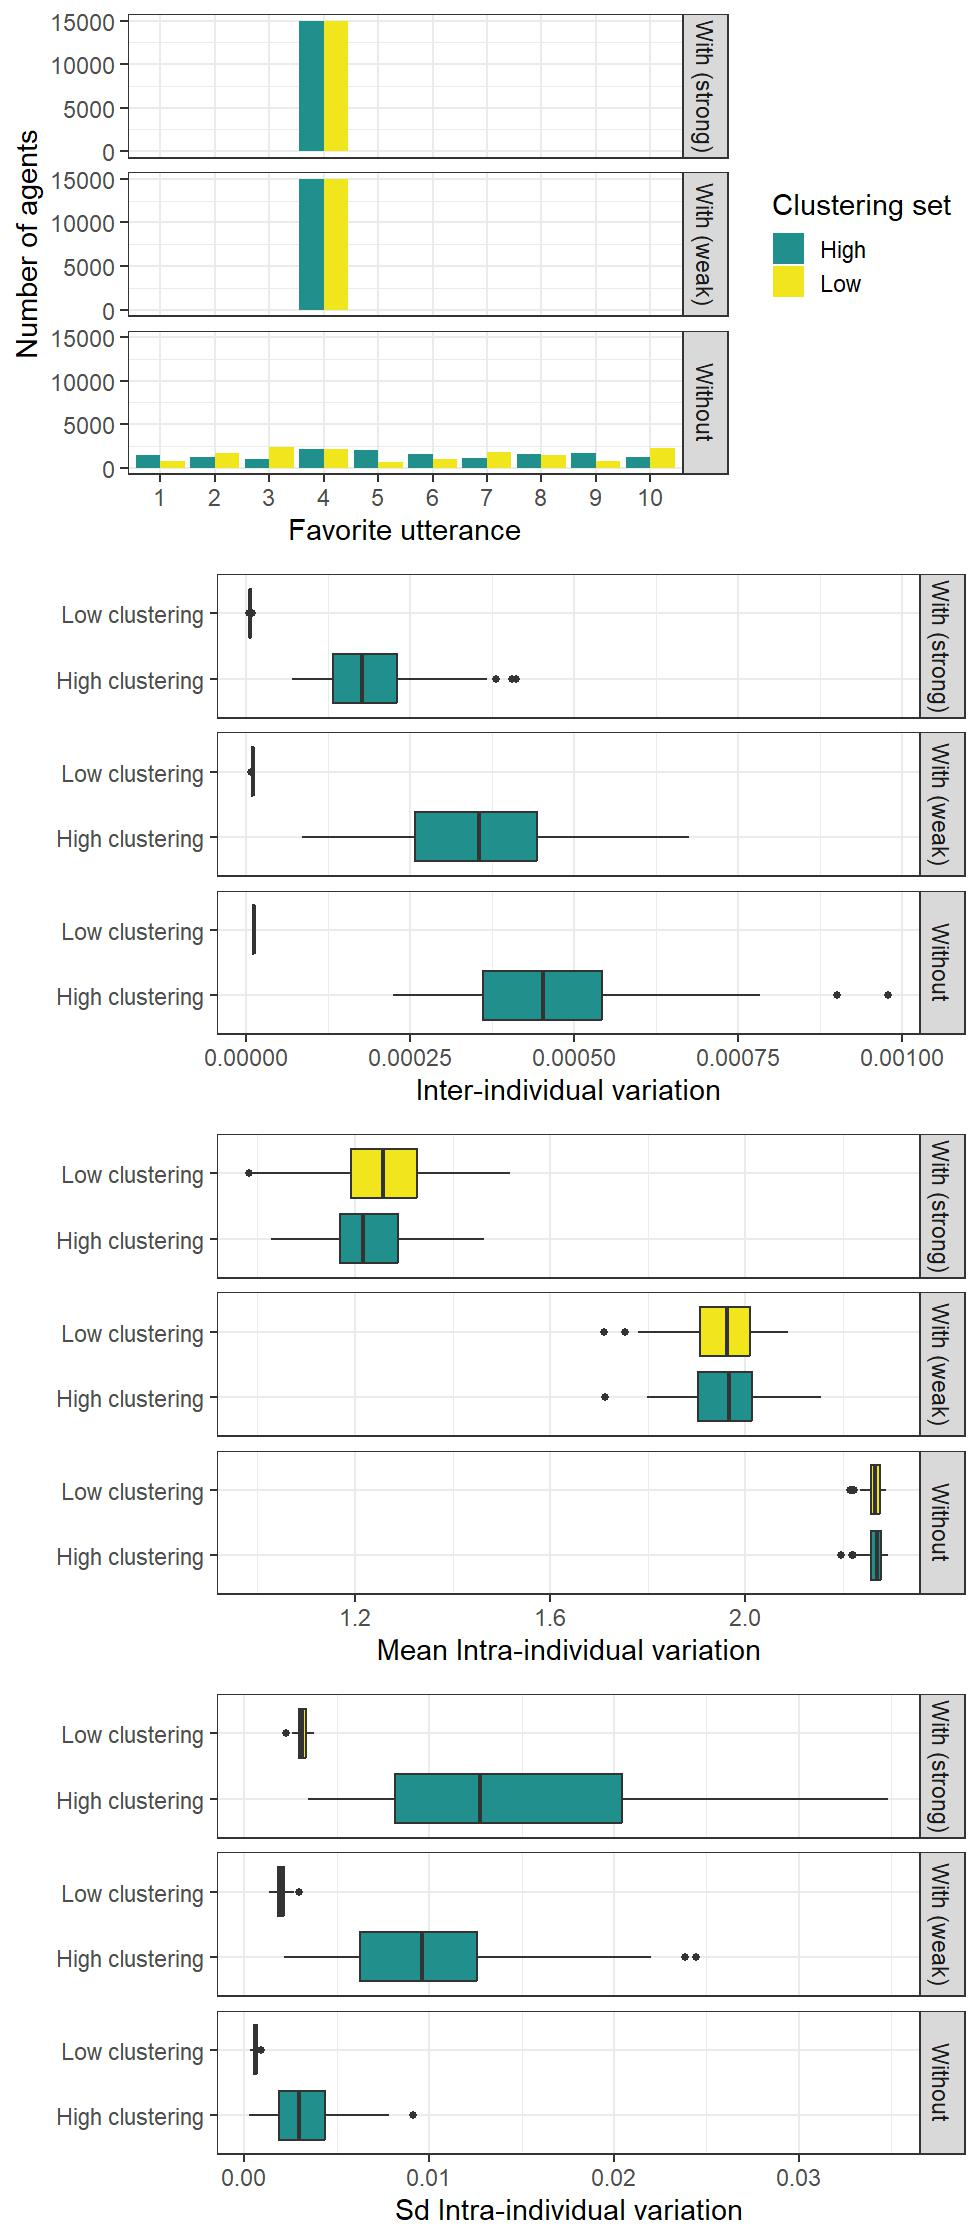
\includegraphics{./Figures/unnamed-chunk-23-1} 

}

\caption{Looking at the variability inter- and intra-individual in sets varying in *clustering*. The first graph shows the value of the language: it shows the favorite utterance for each agents in the three types of population (variable initial language exposure). The second graph shows the  inter-individual variation (the x scale is the average Kullback-Leibler divergence on all pairs of agents). The third and fourth graph show respectively the mean and standard deviation on the intra-individual variation for all agents (the x scale shows respectively the mean and the std of the entropy on the Dirichlet internal representation of agents). In all the following graphs, green shows high value in the metrics while yellow shows low value in the metric.}\label{fig:unnamed-chunk-23}
\end{figure}

Please note that the \texttt{x} scale here is different due to
differences in the network type.

Here, we want to understand whether the effect size under these
differences is high or low.

We apply Cohen's d test and a classic t.test, in networks
\textbf{without} language exposure, \textbf{with (weak)} language
exposure, and \textbf{with (strong)} language exposure. We gathered the
results in a summary table:

Cohen's \emph{D}:

\begin{longtable}[]{@{}
  >{\raggedright\arraybackslash}p{(\columnwidth - 12\tabcolsep) * \real{0.1571}}
  >{\raggedright\arraybackslash}p{(\columnwidth - 12\tabcolsep) * \real{0.2000}}
  >{\raggedright\arraybackslash}p{(\columnwidth - 12\tabcolsep) * \real{0.2000}}
  >{\raggedleft\arraybackslash}p{(\columnwidth - 12\tabcolsep) * \real{0.1000}}
  >{\raggedleft\arraybackslash}p{(\columnwidth - 12\tabcolsep) * \real{0.1429}}
  >{\raggedleft\arraybackslash}p{(\columnwidth - 12\tabcolsep) * \real{0.1000}}
  >{\raggedleft\arraybackslash}p{(\columnwidth - 12\tabcolsep) * \real{0.1000}}@{}}
\toprule()
\begin{minipage}[b]{\linewidth}\raggedright
Measure
\end{minipage} & \begin{minipage}[b]{\linewidth}\raggedright
TypeVariation
\end{minipage} & \begin{minipage}[b]{\linewidth}\raggedright
TypeLangage
\end{minipage} & \begin{minipage}[b]{\linewidth}\raggedleft
CohenD
\end{minipage} & \begin{minipage}[b]{\linewidth}\raggedleft
Magnitude
\end{minipage} & \begin{minipage}[b]{\linewidth}\raggedleft
CI\_Inf
\end{minipage} & \begin{minipage}[b]{\linewidth}\raggedleft
CI\_Sup
\end{minipage} \\
\midrule()
\endhead
clustering & Inter & Without & 4.163 & 4 & 3.667 & 4.660 \\
clustering & Inter & With (weak) & 4.160 & 4 & 3.664 & 4.656 \\
clustering & Inter & With (strong) & 3.420 & 4 & 2.983 & 3.858 \\
clustering & Mean Intra & Without & 0.050 & 1 & -0.229 & 0.329 \\
clustering & Mean Intra & With (weak) & 0.087 & 1 & -0.192 & 0.366 \\
clustering & Mean Intra & With (strong) & 0.296 & 2 & 0.576 & 0.015 \\
clustering & Std Intra & Without & 2.017 & 4 & 1.674 & 2.359 \\
clustering & Std Intra & With (weak) & 2.220 & 4 & 1.866 & 2.575 \\
clustering & Std Intra & With (strong) & 2.070 & 4 & 1.724 & 2.415 \\
\bottomrule()
\end{longtable}

\emph{T}-Test:

\begin{longtable}[]{@{}
  >{\raggedright\arraybackslash}p{(\columnwidth - 14\tabcolsep) * \real{0.1392}}
  >{\raggedright\arraybackslash}p{(\columnwidth - 14\tabcolsep) * \real{0.1772}}
  >{\raggedright\arraybackslash}p{(\columnwidth - 14\tabcolsep) * \real{0.1772}}
  >{\raggedleft\arraybackslash}p{(\columnwidth - 14\tabcolsep) * \real{0.1013}}
  >{\raggedleft\arraybackslash}p{(\columnwidth - 14\tabcolsep) * \real{0.1013}}
  >{\raggedleft\arraybackslash}p{(\columnwidth - 14\tabcolsep) * \real{0.1266}}
  >{\raggedleft\arraybackslash}p{(\columnwidth - 14\tabcolsep) * \real{0.0886}}
  >{\raggedleft\arraybackslash}p{(\columnwidth - 14\tabcolsep) * \real{0.0886}}@{}}
\toprule()
\begin{minipage}[b]{\linewidth}\raggedright
Measure
\end{minipage} & \begin{minipage}[b]{\linewidth}\raggedright
TypeVariation
\end{minipage} & \begin{minipage}[b]{\linewidth}\raggedright
TypeLangage
\end{minipage} & \begin{minipage}[b]{\linewidth}\raggedleft
T\_value
\end{minipage} & \begin{minipage}[b]{\linewidth}\raggedleft
DF
\end{minipage} & \begin{minipage}[b]{\linewidth}\raggedleft
PValue
\end{minipage} & \begin{minipage}[b]{\linewidth}\raggedleft
CI\_Inf
\end{minipage} & \begin{minipage}[b]{\linewidth}\raggedleft
CI\_Sup
\end{minipage} \\
\midrule()
\endhead
clustering & Inter & Without & 29.440 & 99.004 & 0.0000000 & 3.667 &
4.660 \\
clustering & Inter & With (weak) & 29.416 & 99.007 & 0.0000000 & 3.664 &
4.656 \\
clustering & Inter & With (strong) & 24.184 & 99.015 & 0.0000000 & 2.983
& 3.858 \\
clustering & Mean Intra & Without & 0.356 & 193.893 & 0.7223852 & -0.229
& 0.329 \\
clustering & Mean Intra & With (weak) & 0.618 & 197.975 & 0.5369757 &
-0.192 & 0.366 \\
clustering & Mean Intra & With (strong) & -2.092 & 194.149 & 0.0377403 &
-0.576 & -0.015 \\
clustering & Std Intra & Without & 14.259 & 99.958 & 0.0000000 & 1.674 &
2.359 \\
clustering & Std Intra & With (weak) & 15.701 & 99.653 & 0.0000000 &
1.866 & 2.575 \\
clustering & Std Intra & With (strong) & 14.635 & 99.254 & 0.0000000 &
1.724 & 2.415 \\
\bottomrule()
\end{longtable}

\hypertarget{node-degree}{%
\paragraph{Node degree}\label{node-degree}}

These sets of networks were obtained using \textbf{random} networks.

We first observe the values of the two sets:

\begin{longtable}[]{@{}
  >{\raggedright\arraybackslash}p{(\columnwidth - 14\tabcolsep) * \real{0.2234}}
  >{\raggedleft\arraybackslash}p{(\columnwidth - 14\tabcolsep) * \real{0.1170}}
  >{\raggedleft\arraybackslash}p{(\columnwidth - 14\tabcolsep) * \real{0.1064}}
  >{\raggedleft\arraybackslash}p{(\columnwidth - 14\tabcolsep) * \real{0.1170}}
  >{\raggedleft\arraybackslash}p{(\columnwidth - 14\tabcolsep) * \real{0.1489}}
  >{\raggedleft\arraybackslash}p{(\columnwidth - 14\tabcolsep) * \real{0.0957}}
  >{\raggedleft\arraybackslash}p{(\columnwidth - 14\tabcolsep) * \real{0.0532}}
  >{\raggedright\arraybackslash}p{(\columnwidth - 14\tabcolsep) * \real{0.1383}}@{}}
\toprule()
\begin{minipage}[b]{\linewidth}\raggedright
\end{minipage} & \begin{minipage}[b]{\linewidth}\raggedleft
pathlength
\end{minipage} & \begin{minipage}[b]{\linewidth}\raggedleft
neighbors
\end{minipage} & \begin{minipage}[b]{\linewidth}\raggedleft
clustering
\end{minipage} & \begin{minipage}[b]{\linewidth}\raggedleft
assortativity
\end{minipage} & \begin{minipage}[b]{\linewidth}\raggedleft
exponent
\end{minipage} & \begin{minipage}[b]{\linewidth}\raggedleft
size
\end{minipage} & \begin{minipage}[b]{\linewidth}\raggedright
network\_type
\end{minipage} \\
\midrule()
\endhead
Low node degree set & 1.785524 & 11.97893 & 0.2450417 & 0.0138245 & NA &
50 & Random \\
High node degree set & 1.777197 & 12.69280 & 0.2531758 & 0.0249452 & NA
& 50 & Random \\
\bottomrule()
\end{longtable}

This should be interpreted in the following way:

\begin{itemize}
\tightlist
\item
  there is a difference of -0.0068 between the two sets concerning
  \emph{node degree}
\item
  there are differences of 0.0083 for the \emph{clustering} coefficient,
  0.3735 for the \emph{pathlength} coefficient,
  \ensuremath{3\times 10^{-4}} for the \emph{assortativity}, NA for the
  \emph{exponent}, and 0 for the \emph{size}
\end{itemize}

Thus, we compare the differences in inter and intra-individual variation
between the two sets. We believe that these differences will reflect the
differences in node degree, as the other metrics are kept (almost)
constant.

We look at the differences between the two sets:

\begin{figure}[!H]

{\centering 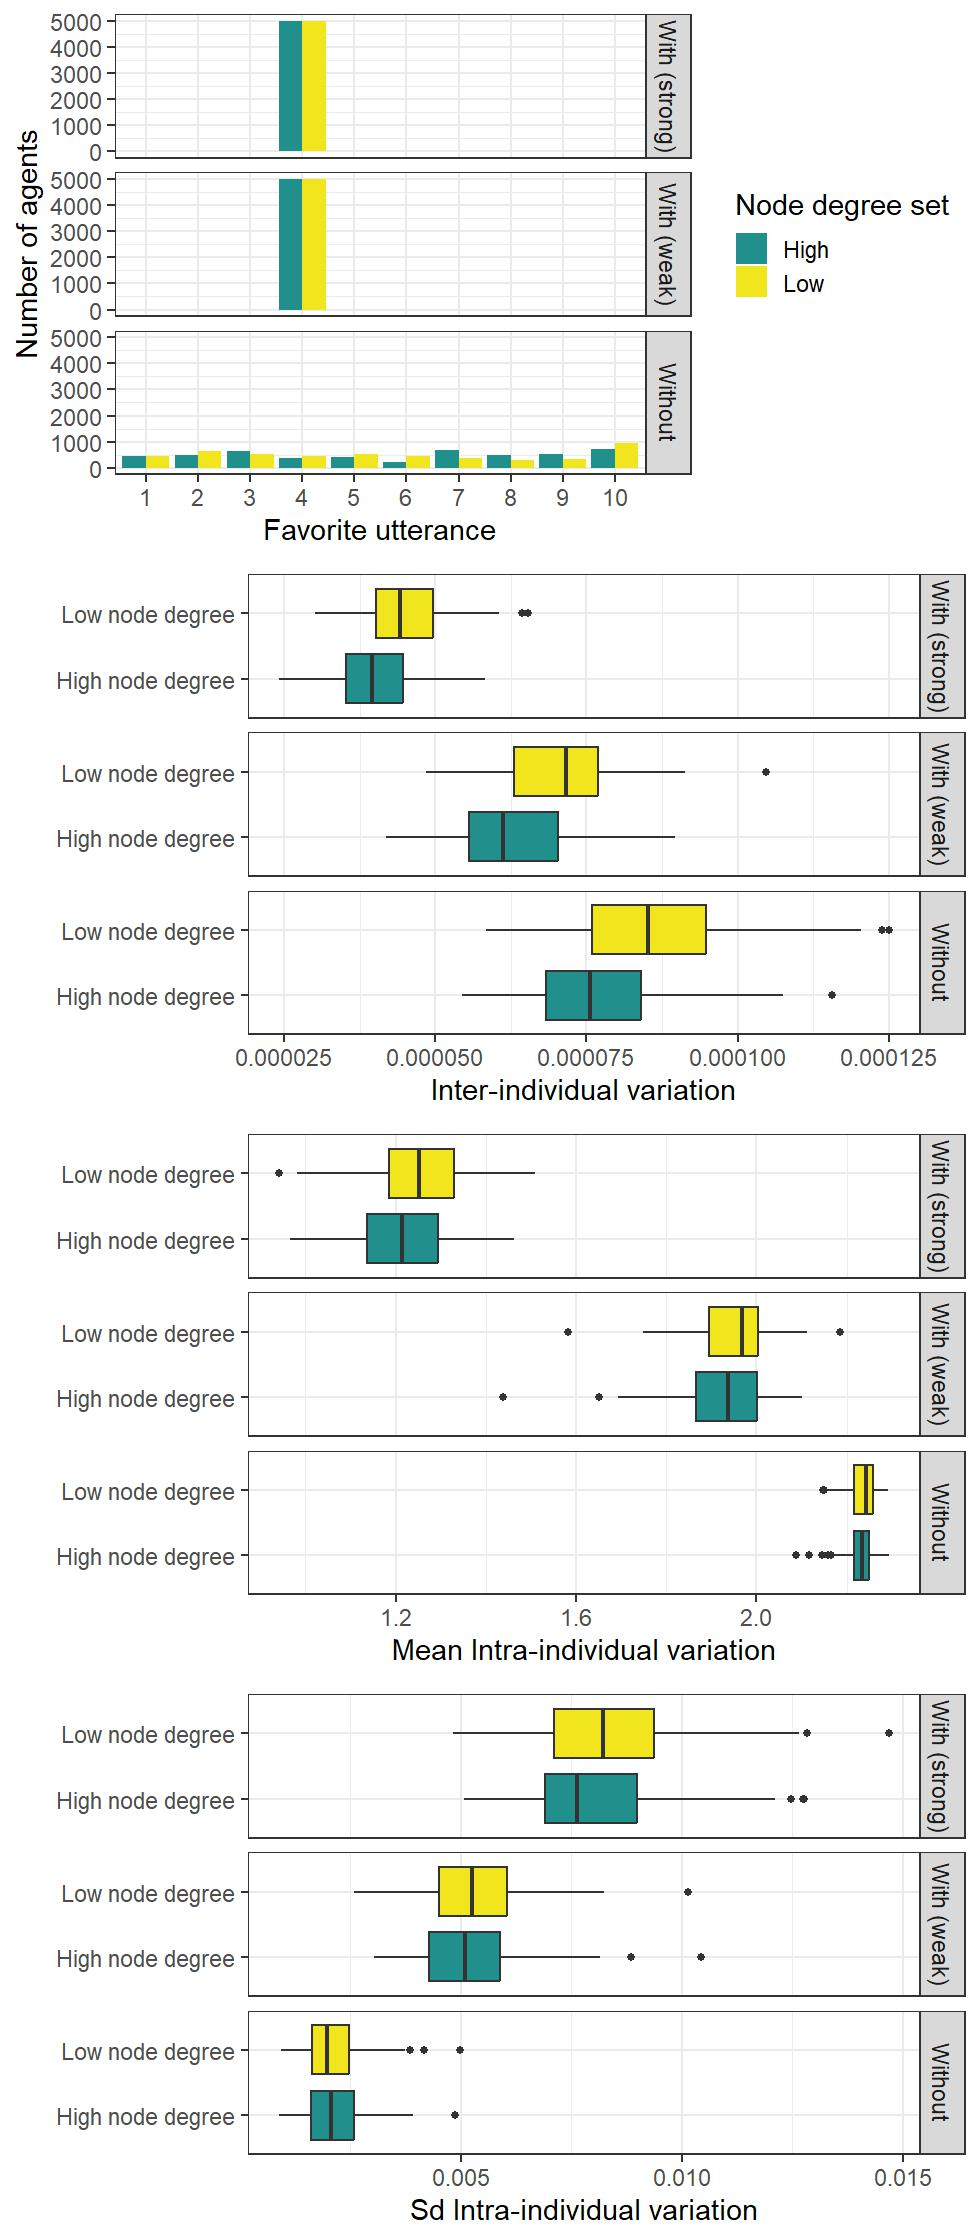
\includegraphics{./Figures/unnamed-chunk-28-1} 

}

\caption{Looking at the variability inter- and intra-individual in sets varying in *node degree*. The first graph shows the value of the language: it shows the favorite utterance for each agents in the three types of population (variable initial language exposure). The second graph shows the  inter-individual variation (the x scale is the average Kullback-Leibler divergence on all pairs of agents). The third and fourth graph show respectively the mean and standard deviation on the intra-individual variation for all agents (the x scale shows respectively the mean and the std of the entropy on the Dirichlet internal representation of agents). In all the following graphs, green shows high value in the metrics while yellow shows low value in the metric.}\label{fig:unnamed-chunk-28}
\end{figure}

Please note that the \texttt{x} scale here is different due to
differences in the network type.

Here, we want to understand whether the effect size under these
differences is high or low.

We apply Cohen's d test and a classic t.test, in networks
\textbf{without} language exposure, \textbf{with (weak)} language
exposure, and \textbf{with (strong)} language exposure. We gathered the
results in a summary table:

\begin{longtable}[]{@{}
  >{\raggedright\arraybackslash}p{(\columnwidth - 12\tabcolsep) * \real{0.1690}}
  >{\raggedright\arraybackslash}p{(\columnwidth - 12\tabcolsep) * \real{0.1972}}
  >{\raggedright\arraybackslash}p{(\columnwidth - 12\tabcolsep) * \real{0.1972}}
  >{\raggedleft\arraybackslash}p{(\columnwidth - 12\tabcolsep) * \real{0.0986}}
  >{\raggedleft\arraybackslash}p{(\columnwidth - 12\tabcolsep) * \real{0.1408}}
  >{\raggedleft\arraybackslash}p{(\columnwidth - 12\tabcolsep) * \real{0.0986}}
  >{\raggedleft\arraybackslash}p{(\columnwidth - 12\tabcolsep) * \real{0.0986}}@{}}
\toprule()
\begin{minipage}[b]{\linewidth}\raggedright
Measure
\end{minipage} & \begin{minipage}[b]{\linewidth}\raggedright
TypeVariation
\end{minipage} & \begin{minipage}[b]{\linewidth}\raggedright
TypeLangage
\end{minipage} & \begin{minipage}[b]{\linewidth}\raggedleft
CohenD
\end{minipage} & \begin{minipage}[b]{\linewidth}\raggedleft
Magnitude
\end{minipage} & \begin{minipage}[b]{\linewidth}\raggedleft
CI\_Inf
\end{minipage} & \begin{minipage}[b]{\linewidth}\raggedleft
CI\_Sup
\end{minipage} \\
\midrule()
\endhead
node\_degree & Inter & Without & 0.708 & 3 & 0.995 & 0.420 \\
node\_degree & Inter & With (weak) & 0.725 & 3 & 1.013 & 0.437 \\
node\_degree & Inter & With (strong) & 0.648 & 3 & 0.935 & 0.362 \\
node\_degree & Mean Intra & Without & 0.140 & 1 & -0.139 & 0.420 \\
node\_degree & Mean Intra & With (weak) & 0.268 & 2 & -0.012 & 0.548 \\
node\_degree & Mean Intra & With (strong) & 0.311 & 2 & 0.592 & 0.031 \\
node\_degree & Std Intra & Without & 0.057 & 1 & -0.222 & 0.336 \\
node\_degree & Std Intra & With (weak) & 0.138 & 1 & -0.141 & 0.418 \\
node\_degree & Std Intra & With (strong) & 0.298 & 2 & 0.578 & 0.017 \\
\bottomrule()
\end{longtable}

\emph{T}-Test:

\begin{longtable}[]{@{}
  >{\raggedright\arraybackslash}p{(\columnwidth - 14\tabcolsep) * \real{0.1500}}
  >{\raggedright\arraybackslash}p{(\columnwidth - 14\tabcolsep) * \real{0.1750}}
  >{\raggedright\arraybackslash}p{(\columnwidth - 14\tabcolsep) * \real{0.1750}}
  >{\raggedleft\arraybackslash}p{(\columnwidth - 14\tabcolsep) * \real{0.1000}}
  >{\raggedleft\arraybackslash}p{(\columnwidth - 14\tabcolsep) * \real{0.1000}}
  >{\raggedleft\arraybackslash}p{(\columnwidth - 14\tabcolsep) * \real{0.1250}}
  >{\raggedleft\arraybackslash}p{(\columnwidth - 14\tabcolsep) * \real{0.0875}}
  >{\raggedleft\arraybackslash}p{(\columnwidth - 14\tabcolsep) * \real{0.0875}}@{}}
\toprule()
\begin{minipage}[b]{\linewidth}\raggedright
Measure
\end{minipage} & \begin{minipage}[b]{\linewidth}\raggedright
TypeVariation
\end{minipage} & \begin{minipage}[b]{\linewidth}\raggedright
TypeLangage
\end{minipage} & \begin{minipage}[b]{\linewidth}\raggedleft
T\_value
\end{minipage} & \begin{minipage}[b]{\linewidth}\raggedleft
DF
\end{minipage} & \begin{minipage}[b]{\linewidth}\raggedleft
PValue
\end{minipage} & \begin{minipage}[b]{\linewidth}\raggedleft
CI\_Inf
\end{minipage} & \begin{minipage}[b]{\linewidth}\raggedleft
CI\_Sup
\end{minipage} \\
\midrule()
\endhead
node\_degree & Inter & Without & -5.006 & 191.822 & 0.0000013 & -0.995 &
-0.420 \\
node\_degree & Inter & With (weak) & -5.125 & 197.972 & 0.0000007 &
-1.013 & -0.437 \\
node\_degree & Inter & With (strong) & -4.585 & 195.159 & 0.0000081 &
-0.935 & -0.362 \\
node\_degree & Mean Intra & Without & -0.987 & 197.253 & 0.3248058 &
-0.419 & 0.140 \\
node\_degree & Mean Intra & With (weak) & -1.894 & 191.699 & 0.0597234 &
-0.548 & 0.012 \\
node\_degree & Mean Intra & With (strong) & -2.202 & 197.439 & 0.0288564
& -0.592 & -0.031 \\
node\_degree & Std Intra & Without & 0.406 & 196.701 & 0.6854013 &
-0.222 & 0.336 \\
node\_degree & Std Intra & With (weak) & -0.974 & 197.709 & 0.3313699 &
-0.417 & 0.142 \\
node\_degree & Std Intra & With (strong) & -2.105 & 191.655 & 0.0365533
& -0.578 & -0.017 \\
\bottomrule()
\end{longtable}

\hypertarget{pathlength-using-random}{%
\paragraph{Pathlength (using random)}\label{pathlength-using-random}}

These sets of networks were obtained using \textbf{random} networks.
Pathlength was already explored using \emph{scale-free} networks, and
controlling for many metrics Here, we just want to observe the effect of
\emph{pathlength} in opposite to the effect of \emph{mean degree}, in
random network.

We first observe the values of the two sets:

\begin{longtable}[]{@{}
  >{\raggedright\arraybackslash}p{(\columnwidth - 14\tabcolsep) * \real{0.2151}}
  >{\raggedleft\arraybackslash}p{(\columnwidth - 14\tabcolsep) * \real{0.1183}}
  >{\raggedleft\arraybackslash}p{(\columnwidth - 14\tabcolsep) * \real{0.1075}}
  >{\raggedleft\arraybackslash}p{(\columnwidth - 14\tabcolsep) * \real{0.1183}}
  >{\raggedleft\arraybackslash}p{(\columnwidth - 14\tabcolsep) * \real{0.1505}}
  >{\raggedleft\arraybackslash}p{(\columnwidth - 14\tabcolsep) * \real{0.0968}}
  >{\raggedleft\arraybackslash}p{(\columnwidth - 14\tabcolsep) * \real{0.0538}}
  >{\raggedright\arraybackslash}p{(\columnwidth - 14\tabcolsep) * \real{0.1398}}@{}}
\toprule()
\begin{minipage}[b]{\linewidth}\raggedright
\end{minipage} & \begin{minipage}[b]{\linewidth}\raggedleft
pathlength
\end{minipage} & \begin{minipage}[b]{\linewidth}\raggedleft
neighbors
\end{minipage} & \begin{minipage}[b]{\linewidth}\raggedleft
clustering
\end{minipage} & \begin{minipage}[b]{\linewidth}\raggedleft
assortativity
\end{minipage} & \begin{minipage}[b]{\linewidth}\raggedleft
exponent
\end{minipage} & \begin{minipage}[b]{\linewidth}\raggedleft
size
\end{minipage} & \begin{minipage}[b]{\linewidth}\raggedright
network\_type
\end{minipage} \\
\midrule()
\endhead
Low pathlength set & 4.314229 & 2.467467 & 0.0285249 & -0.1041842 & NA &
50 & Random \\
High pathlength set & 4.314229 & 2.467467 & 0.0285249 & -0.1041842 & NA
& 50 & Random \\
\bottomrule()
\end{longtable}

This should be interpreted in the following way:

\begin{itemize}
\tightlist
\item
  there is a difference of 0.3735 between the two sets concerning
  \emph{pathlength}
\item
  there are differences of 0.0083 for the \emph{clustering} coefficient,
  -0.0068 for the \emph{node degree} coefficient,
  \ensuremath{3\times 10^{-4}} for the \emph{assortativity}, and 0 for
  the \emph{size}
\end{itemize}

Thus, we compare the differences in inter and intra-individual variation
between the two sets. We believe that these differences will reflect the
differences in node degree, as the other metrics are kept (almost)
constant.

We look at the differences between the two sets:

\begin{figure}[!H]

{\centering 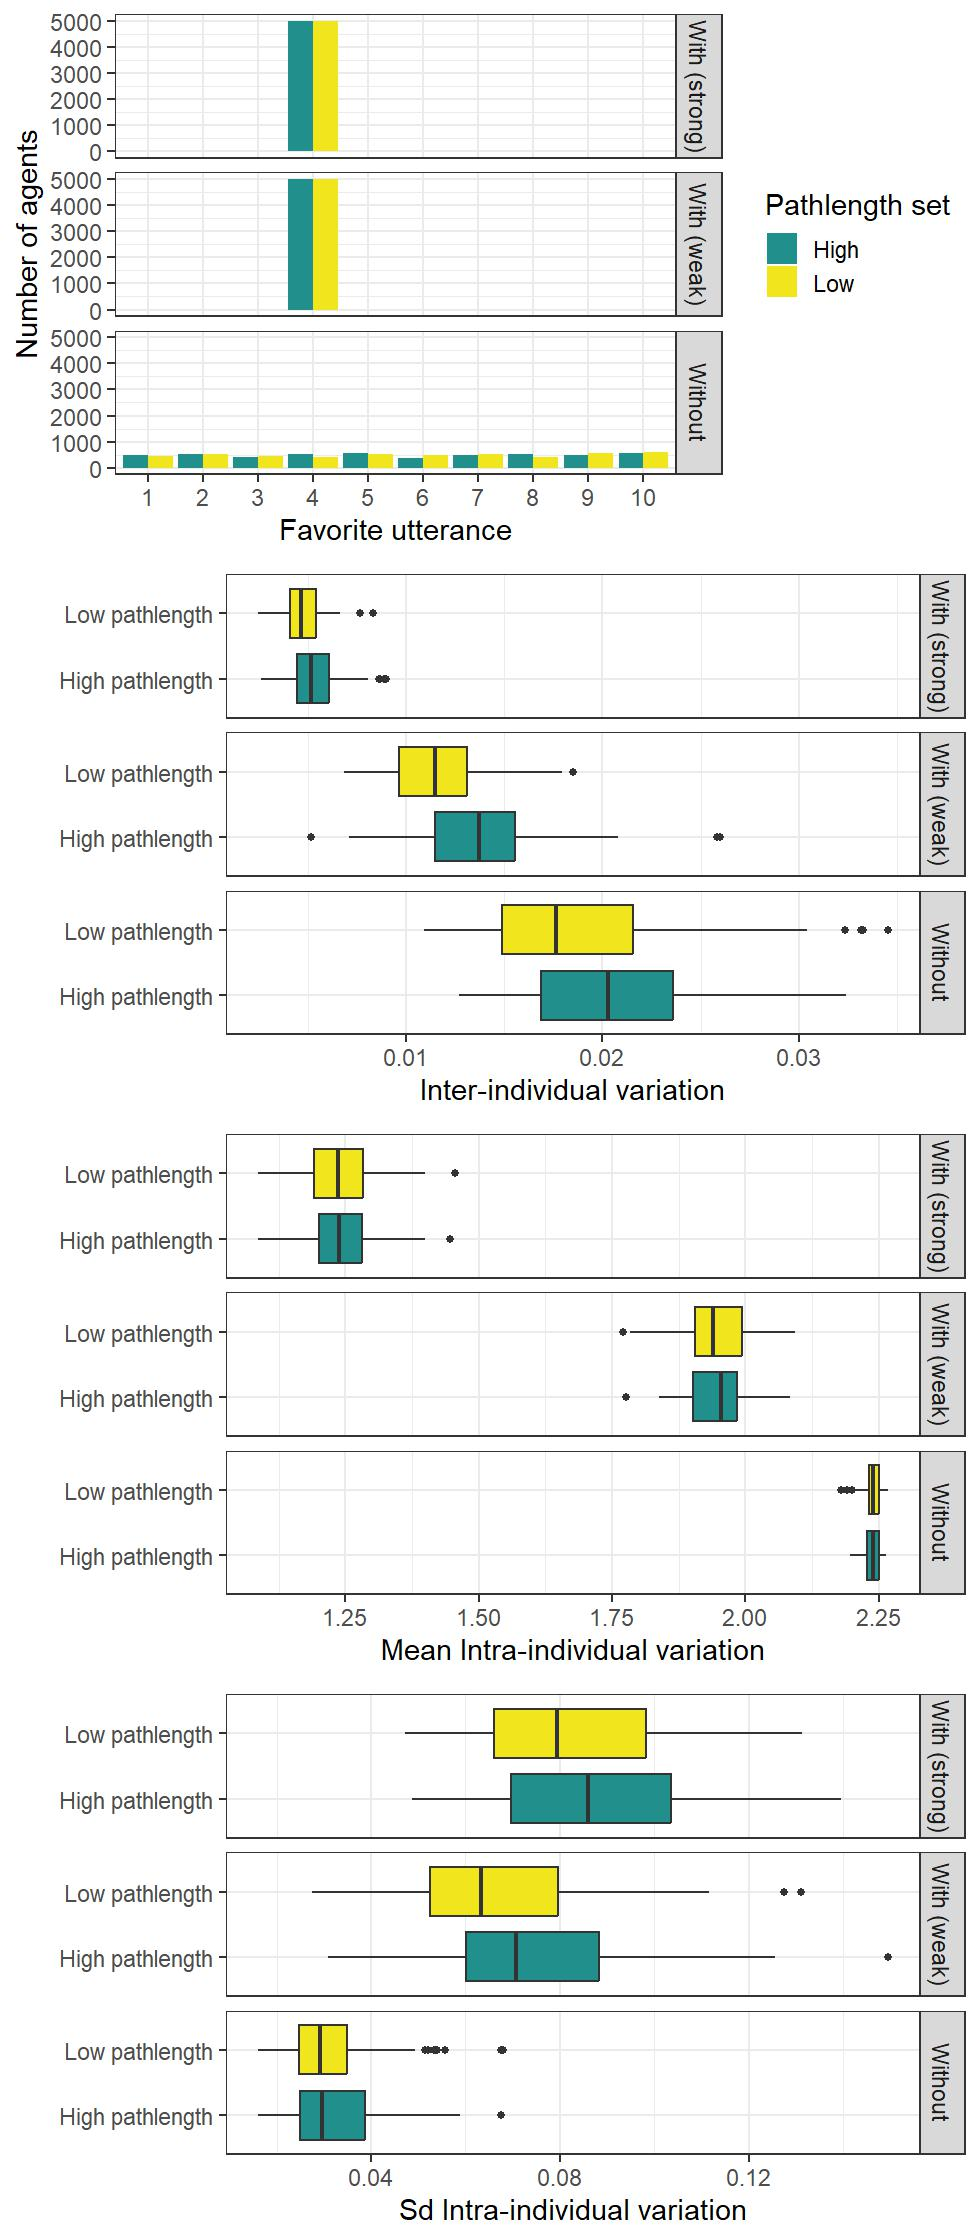
\includegraphics{./Figures/unnamed-chunk-32-1} 

}

\caption{Looking at the variability inter- and intra-individual in sets varying in *pathlength* (using random networks, and not scale-free networks). The first graph shows the value of the language: it shows the favorite utterance for each agents in the three types of population (variable initial language exposure). The second graph shows the  inter-individual variation (the x scale is the average Kullback-Leibler divergence on all pairs of agents). The third and fourth graph show respectively the mean and standard deviation on the intra-individual variation for all agents (the x scale shows respectively the mean and the std of the entropy on the Dirichlet internal representation of agents). In all the following graphs, green shows high value in the metrics while yellow shows low value in the metric.}\label{fig:unnamed-chunk-32}
\end{figure}

Please note that the \texttt{x} scale here is different due to
differences in the network type.

Here, we want to understand whether the effect size under these
differences is high or low.

We apply Cohen's d test and a classic t.test, in networks
\textbf{without} language exposure, \textbf{with (weak)} language
exposure, and \textbf{with (strong)} language exposure. We gathered the
results in a summary table:

Cohen's \emph{D}:

\begin{longtable}[]{@{}
  >{\raggedright\arraybackslash}p{(\columnwidth - 12\tabcolsep) * \real{0.2027}}
  >{\raggedright\arraybackslash}p{(\columnwidth - 12\tabcolsep) * \real{0.1892}}
  >{\raggedright\arraybackslash}p{(\columnwidth - 12\tabcolsep) * \real{0.1892}}
  >{\raggedleft\arraybackslash}p{(\columnwidth - 12\tabcolsep) * \real{0.0946}}
  >{\raggedleft\arraybackslash}p{(\columnwidth - 12\tabcolsep) * \real{0.1351}}
  >{\raggedleft\arraybackslash}p{(\columnwidth - 12\tabcolsep) * \real{0.0946}}
  >{\raggedleft\arraybackslash}p{(\columnwidth - 12\tabcolsep) * \real{0.0946}}@{}}
\toprule()
\begin{minipage}[b]{\linewidth}\raggedright
Measure
\end{minipage} & \begin{minipage}[b]{\linewidth}\raggedright
TypeVariation
\end{minipage} & \begin{minipage}[b]{\linewidth}\raggedright
TypeLangage
\end{minipage} & \begin{minipage}[b]{\linewidth}\raggedleft
CohenD
\end{minipage} & \begin{minipage}[b]{\linewidth}\raggedleft
Magnitude
\end{minipage} & \begin{minipage}[b]{\linewidth}\raggedleft
CI\_Inf
\end{minipage} & \begin{minipage}[b]{\linewidth}\raggedleft
CI\_Sup
\end{minipage} \\
\midrule()
\endhead
pathlength\_ran & Inter & Without & 0.427 & 2 & 0.145 & 0.709 \\
pathlength\_ran & Inter & With (weak) & 0.727 & 3 & 0.439 & 1.014 \\
pathlength\_ran & Inter & With (strong) & 0.512 & 3 & 0.229 & 0.796 \\
pathlength\_ran & Mean Intra & Without & 0.001 & 1 & -0.278 & 0.279 \\
pathlength\_ran & Mean Intra & With (weak) & 0.000 & 1 & 0.279 &
0.279 \\
pathlength\_ran & Mean Intra & With (strong) & 0.023 & 1 & -0.256 &
0.302 \\
pathlength\_ran & Std Intra & Without & 0.134 & 1 & -0.145 & 0.413 \\
pathlength\_ran & Std Intra & With (weak) & 0.380 & 2 & 0.099 & 0.661 \\
pathlength\_ran & Std Intra & With (strong) & 0.265 & 2 & -0.015 &
0.545 \\
\bottomrule()
\end{longtable}

\emph{T}-Test:

\begin{longtable}[]{@{}
  >{\raggedright\arraybackslash}p{(\columnwidth - 14\tabcolsep) * \real{0.1807}}
  >{\raggedright\arraybackslash}p{(\columnwidth - 14\tabcolsep) * \real{0.1687}}
  >{\raggedright\arraybackslash}p{(\columnwidth - 14\tabcolsep) * \real{0.1687}}
  >{\raggedleft\arraybackslash}p{(\columnwidth - 14\tabcolsep) * \real{0.0964}}
  >{\raggedleft\arraybackslash}p{(\columnwidth - 14\tabcolsep) * \real{0.0964}}
  >{\raggedleft\arraybackslash}p{(\columnwidth - 14\tabcolsep) * \real{0.1205}}
  >{\raggedleft\arraybackslash}p{(\columnwidth - 14\tabcolsep) * \real{0.0843}}
  >{\raggedleft\arraybackslash}p{(\columnwidth - 14\tabcolsep) * \real{0.0843}}@{}}
\toprule()
\begin{minipage}[b]{\linewidth}\raggedright
Measure
\end{minipage} & \begin{minipage}[b]{\linewidth}\raggedright
TypeVariation
\end{minipage} & \begin{minipage}[b]{\linewidth}\raggedright
TypeLangage
\end{minipage} & \begin{minipage}[b]{\linewidth}\raggedleft
T\_value
\end{minipage} & \begin{minipage}[b]{\linewidth}\raggedleft
DF
\end{minipage} & \begin{minipage}[b]{\linewidth}\raggedleft
PValue
\end{minipage} & \begin{minipage}[b]{\linewidth}\raggedleft
CI\_Inf
\end{minipage} & \begin{minipage}[b]{\linewidth}\raggedleft
CI\_Sup
\end{minipage} \\
\midrule()
\endhead
pathlength\_ran & Inter & Without & 3.022 & 196.497 & 0.0028414 & 0.145
& 0.709 \\
pathlength\_ran & Inter & With (weak) & 5.137 & 183.653 & 0.0000007 &
0.439 & 1.014 \\
pathlength\_ran & Inter & With (strong) & 3.623 & 185.944 & 0.0003750 &
0.229 & 0.796 \\
pathlength\_ran & Mean Intra & Without & 0.004 & 193.154 & 0.9969390 &
-0.278 & 0.279 \\
pathlength\_ran & Mean Intra & With (weak) & 0.001 & 192.635 & 0.9990379
& -0.279 & 0.279 \\
pathlength\_ran & Mean Intra & With (strong) & 0.161 & 196.648 &
0.8721028 & -0.256 & 0.302 \\
pathlength\_ran & Std Intra & Without & 0.949 & 198.000 & 0.3438721 &
-0.145 & 0.413 \\
pathlength\_ran & Std Intra & With (weak) & 2.686 & 196.273 & 0.0078432
& 0.099 & 0.661 \\
pathlength\_ran & Std Intra & With (strong) & 1.872 & 196.351 &
0.0627478 & -0.015 & 0.545 \\
\bottomrule()
\end{longtable}

\hypertarget{summary-multinomial}{%
\paragraph{Summary multinomial}\label{summary-multinomial}}

Plot with full data:

\begin{center}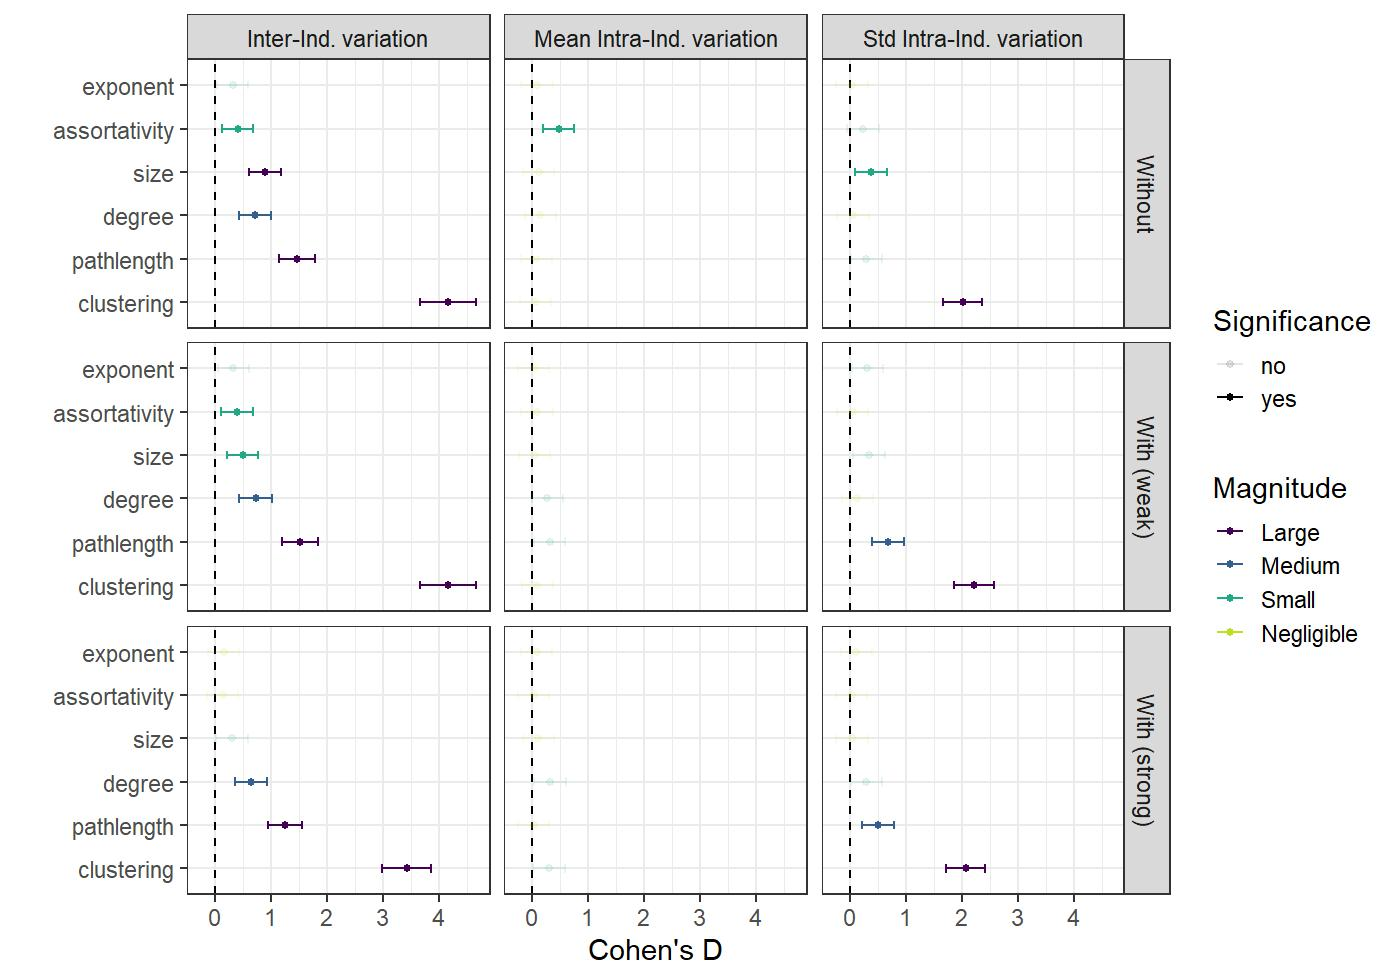
\includegraphics{./Figures/unnamed-chunk-35-1} \end{center}

You can find below the plot used in the main paper, which shows exactly
the same information except that we do not present the results for
\emph{initial language exposure} = \emph{With (Strong)}. Also, we
renamed the \emph{initial language exposure} with type of language
scenario (\emph{without initial language exposure} -\textgreater{}
Language emergence and \emph{with (weak) initial language exposure}
-\textgreater{} Language change). See
\protect\hyperlink{note-on-initial-language-exposure-terminology}{Note
on Initial language exposure terminology} for more information.

\begin{center}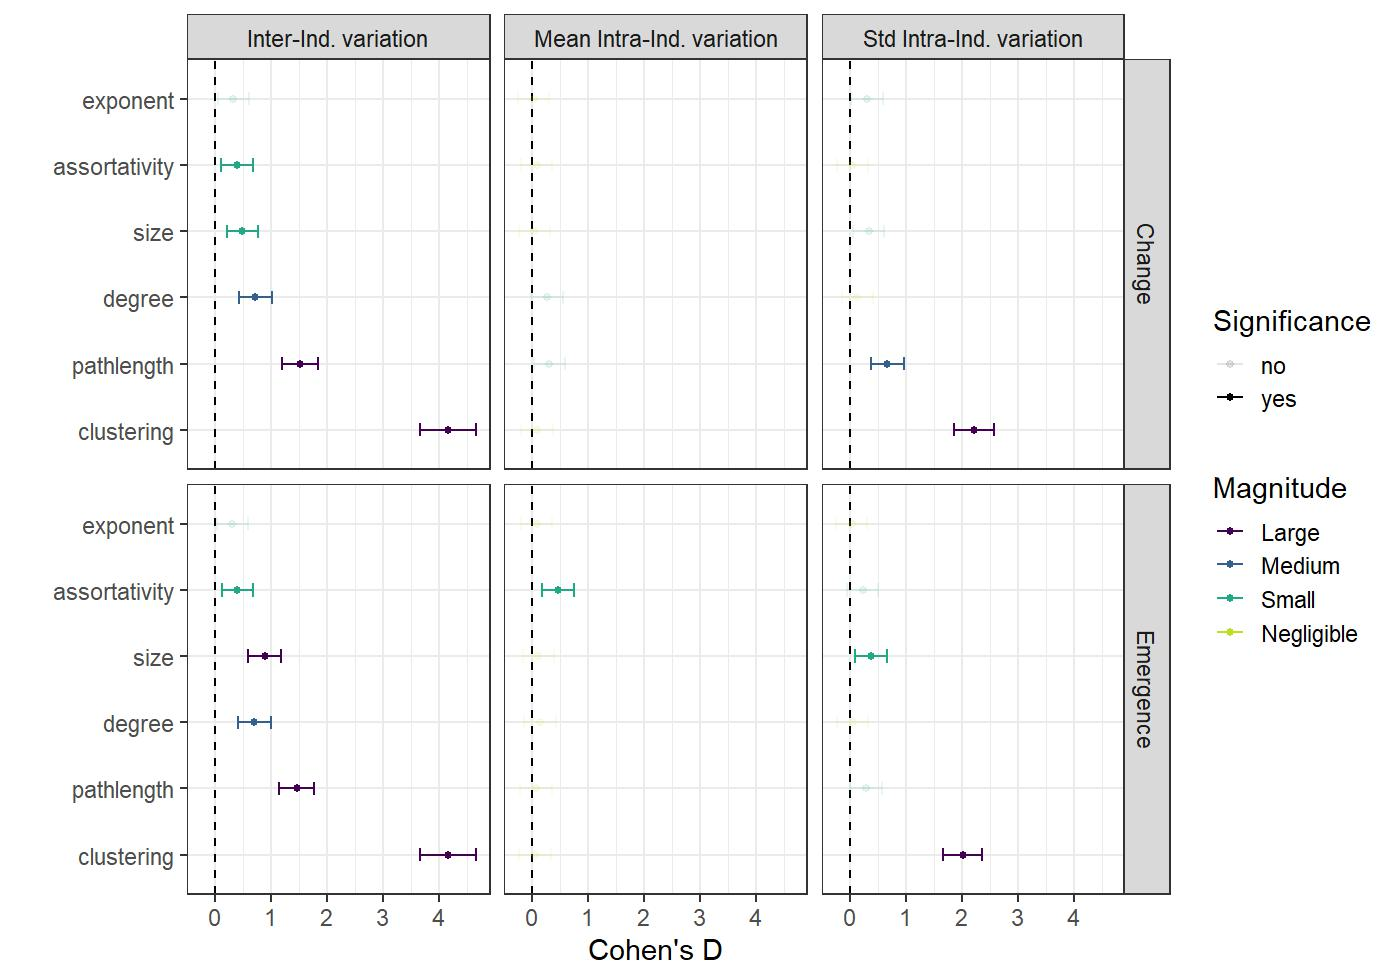
\includegraphics{./Figures/unnamed-chunk-36-1} \end{center}

\hypertarget{continuous-1}{%
\subsubsection{Continuous}\label{continuous-1}}

This part shows exactly the same type of results, except that here
language is continuous and not multinomial. We present the detailed
results for each metric. However, you can refer to the
\protect\hyperlink{summary-continuous}{Summary continuous} part, where
you can see all the information in one plot.

\hypertarget{pathlength-1}{%
\paragraph{Pathlength}\label{pathlength-1}}

These sets of networks were obtained using \textbf{scale-free} networks.

We first observe the values of the two sets:

\begin{longtable}[]{@{}
  >{\raggedright\arraybackslash}p{(\columnwidth - 14\tabcolsep) * \real{0.2151}}
  >{\raggedleft\arraybackslash}p{(\columnwidth - 14\tabcolsep) * \real{0.1183}}
  >{\raggedleft\arraybackslash}p{(\columnwidth - 14\tabcolsep) * \real{0.1075}}
  >{\raggedleft\arraybackslash}p{(\columnwidth - 14\tabcolsep) * \real{0.1183}}
  >{\raggedleft\arraybackslash}p{(\columnwidth - 14\tabcolsep) * \real{0.1505}}
  >{\raggedleft\arraybackslash}p{(\columnwidth - 14\tabcolsep) * \real{0.0968}}
  >{\raggedleft\arraybackslash}p{(\columnwidth - 14\tabcolsep) * \real{0.0538}}
  >{\raggedright\arraybackslash}p{(\columnwidth - 14\tabcolsep) * \real{0.1398}}@{}}
\toprule()
\begin{minipage}[b]{\linewidth}\raggedright
\end{minipage} & \begin{minipage}[b]{\linewidth}\raggedleft
pathlength
\end{minipage} & \begin{minipage}[b]{\linewidth}\raggedleft
neighbors
\end{minipage} & \begin{minipage}[b]{\linewidth}\raggedleft
clustering
\end{minipage} & \begin{minipage}[b]{\linewidth}\raggedleft
assortativity
\end{minipage} & \begin{minipage}[b]{\linewidth}\raggedleft
exponent
\end{minipage} & \begin{minipage}[b]{\linewidth}\raggedleft
size
\end{minipage} & \begin{minipage}[b]{\linewidth}\raggedright
network\_type
\end{minipage} \\
\midrule()
\endhead
Low pathlength set & 3.392992 & 2 & 0 & -0.3101820 & 2.783516 & 50 &
Scalefree \\
High pathlength set & 4.982433 & 2 & 0 & -0.3068284 & 2.770500 & 50 &
Scalefree \\
\bottomrule()
\end{longtable}

This should be interpreted in the following way:

\begin{itemize}
\tightlist
\item
  there is a difference of 1.5894 between the two sets concerning
  \emph{pathlength}
\item
  there are differences of 0 for the \emph{neighbors}, 0 for the
  \emph{clustering} coefficient, 0.0034 for the \emph{assortativity},
  -0.013 for the \emph{exponent}, and 0 for the \emph{size}
\end{itemize}

Thus, we compare the differences in inter and intra-individual variation
between the two sets. We believe that these differences will reflect the
differences in pathlength, as the other metrics are kept (almost)
constant.

We look at the differences between the two sets:

\begin{figure}[!H]

{\centering 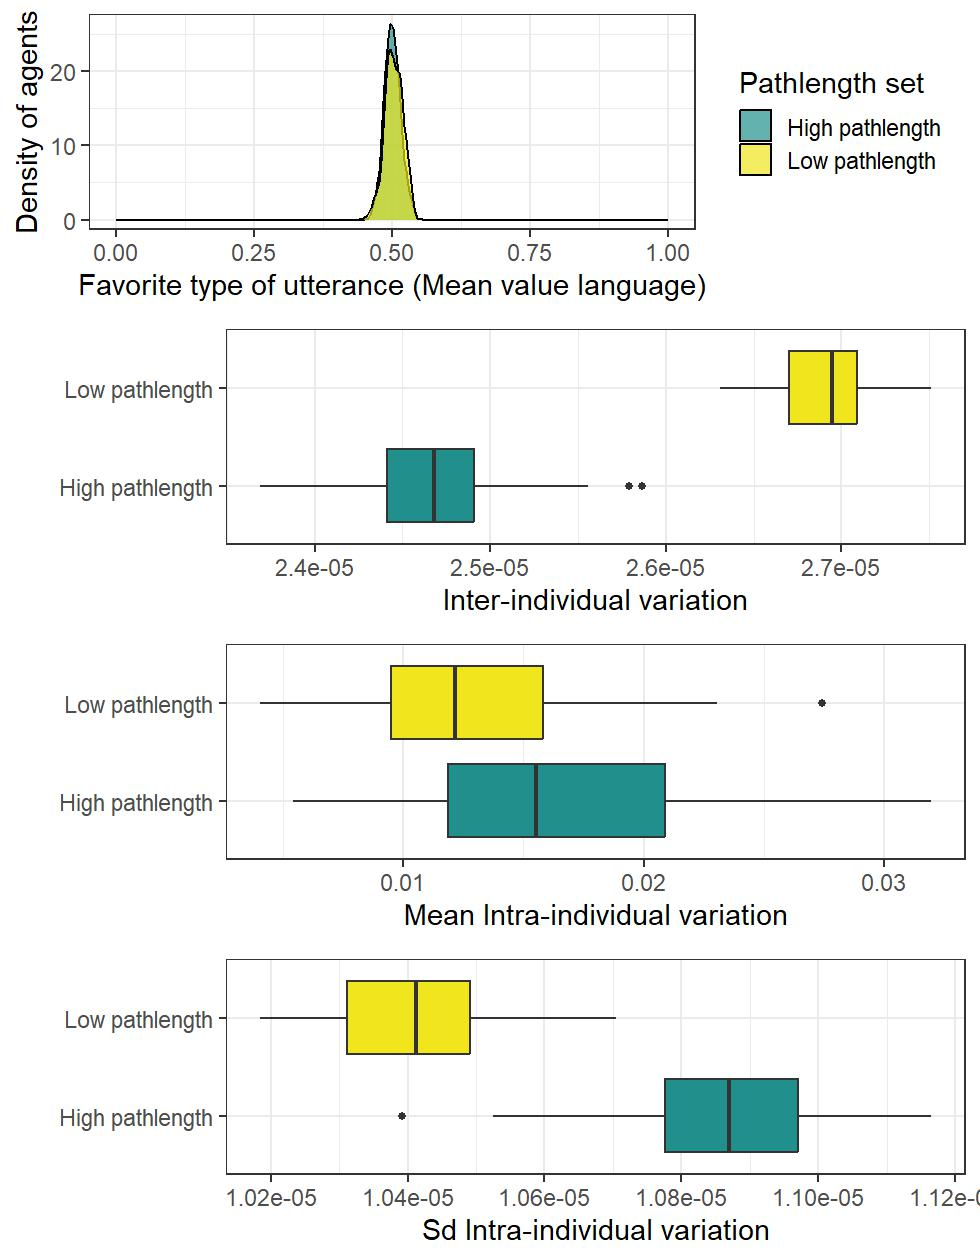
\includegraphics{./Figures/unnamed-chunk-40-1} 

}

\caption{Looking at the variability inter- and intra-individual in sets varying in *pathlength* in network with a continuous language. The first graph shows the value of the language: it shows the favorite utterance for each agents in the three types of population (variable initial language exposure). The second graph shows the  inter-individual variation (the x scale is the average Kullback-Leibler divergence on all pairs of agents). The third and fourth graph show respectively the mean and standard deviation on the intra-individual variation for all agents (the x scale shows respectively the mean and the std of the entropy on the Dirichlet internal representation of agents). In all the following graphs, green shows high value in the metrics while yellow shows low value in the metric.}\label{fig:unnamed-chunk-40}
\end{figure}

Here, we want to understand whether the effect size under these
differences is high or low.

We apply Cohen's d test and a classic t.test, in networks
\textbf{without} language exposure, \textbf{with (weak)} language
exposure, and \textbf{with (strong)} language exposure. We gathered the
results in a summary table:

Cohen's \emph{D}:

\begin{longtable}[]{@{}
  >{\raggedright\arraybackslash}p{(\columnwidth - 12\tabcolsep) * \real{0.1618}}
  >{\raggedright\arraybackslash}p{(\columnwidth - 12\tabcolsep) * \real{0.2059}}
  >{\raggedright\arraybackslash}p{(\columnwidth - 12\tabcolsep) * \real{0.1765}}
  >{\raggedleft\arraybackslash}p{(\columnwidth - 12\tabcolsep) * \real{0.1029}}
  >{\raggedright\arraybackslash}p{(\columnwidth - 12\tabcolsep) * \real{0.1471}}
  >{\raggedleft\arraybackslash}p{(\columnwidth - 12\tabcolsep) * \real{0.1029}}
  >{\raggedleft\arraybackslash}p{(\columnwidth - 12\tabcolsep) * \real{0.1029}}@{}}
\toprule()
\begin{minipage}[b]{\linewidth}\raggedright
Measure
\end{minipage} & \begin{minipage}[b]{\linewidth}\raggedright
TypeVariation
\end{minipage} & \begin{minipage}[b]{\linewidth}\raggedright
TypeLangage
\end{minipage} & \begin{minipage}[b]{\linewidth}\raggedleft
CohenD
\end{minipage} & \begin{minipage}[b]{\linewidth}\raggedright
Magnitude
\end{minipage} & \begin{minipage}[b]{\linewidth}\raggedleft
CI\_Inf
\end{minipage} & \begin{minipage}[b]{\linewidth}\raggedleft
CI\_Sup
\end{minipage} \\
\midrule()
\endhead
pathlength & Inter & None & 6.427 & large & 7.119 & 5.734 \\
pathlength & Mean Intra & None & 0.676 & medium & 0.389 & 0.963 \\
pathlength & Std Intra & None & 3.292 & large & 2.864 & 3.720 \\
\bottomrule()
\end{longtable}

\emph{T}-Test:

\begin{longtable}[]{@{}
  >{\raggedright\arraybackslash}p{(\columnwidth - 14\tabcolsep) * \real{0.1467}}
  >{\raggedright\arraybackslash}p{(\columnwidth - 14\tabcolsep) * \real{0.1867}}
  >{\raggedright\arraybackslash}p{(\columnwidth - 14\tabcolsep) * \real{0.1600}}
  >{\raggedleft\arraybackslash}p{(\columnwidth - 14\tabcolsep) * \real{0.1067}}
  >{\raggedleft\arraybackslash}p{(\columnwidth - 14\tabcolsep) * \real{0.1067}}
  >{\raggedleft\arraybackslash}p{(\columnwidth - 14\tabcolsep) * \real{0.1067}}
  >{\raggedleft\arraybackslash}p{(\columnwidth - 14\tabcolsep) * \real{0.0933}}
  >{\raggedleft\arraybackslash}p{(\columnwidth - 14\tabcolsep) * \real{0.0933}}@{}}
\toprule()
\begin{minipage}[b]{\linewidth}\raggedright
Measure
\end{minipage} & \begin{minipage}[b]{\linewidth}\raggedright
TypeVariation
\end{minipage} & \begin{minipage}[b]{\linewidth}\raggedright
TypeLangage
\end{minipage} & \begin{minipage}[b]{\linewidth}\raggedleft
T\_value
\end{minipage} & \begin{minipage}[b]{\linewidth}\raggedleft
DF
\end{minipage} & \begin{minipage}[b]{\linewidth}\raggedleft
PValue
\end{minipage} & \begin{minipage}[b]{\linewidth}\raggedleft
CI\_Inf
\end{minipage} & \begin{minipage}[b]{\linewidth}\raggedleft
CI\_Sup
\end{minipage} \\
\midrule()
\endhead
pathlength & Inter & None & -45.444 & 171.791 & 0.0e+00 & 7.119 &
5.734 \\
pathlength & Mean Intra & None & 4.781 & 187.838 & 3.5e-06 & 0.389 &
0.963 \\
pathlength & Std Intra & None & 23.279 & 189.202 & 0.0e+00 & 2.864 &
3.720 \\
\bottomrule()
\end{longtable}

\hypertarget{assortativity-1}{%
\paragraph{Assortativity}\label{assortativity-1}}

These sets of networks were obtained using \textbf{scale-free} networks.

We first observe the values of the two sets:

\begin{longtable}[]{@{}
  >{\raggedright\arraybackslash}p{(\columnwidth - 14\tabcolsep) * \real{0.2396}}
  >{\raggedleft\arraybackslash}p{(\columnwidth - 14\tabcolsep) * \real{0.1146}}
  >{\raggedleft\arraybackslash}p{(\columnwidth - 14\tabcolsep) * \real{0.1042}}
  >{\raggedleft\arraybackslash}p{(\columnwidth - 14\tabcolsep) * \real{0.1146}}
  >{\raggedleft\arraybackslash}p{(\columnwidth - 14\tabcolsep) * \real{0.1458}}
  >{\raggedleft\arraybackslash}p{(\columnwidth - 14\tabcolsep) * \real{0.0937}}
  >{\raggedleft\arraybackslash}p{(\columnwidth - 14\tabcolsep) * \real{0.0521}}
  >{\raggedright\arraybackslash}p{(\columnwidth - 14\tabcolsep) * \real{0.1354}}@{}}
\toprule()
\begin{minipage}[b]{\linewidth}\raggedright
\end{minipage} & \begin{minipage}[b]{\linewidth}\raggedleft
pathlength
\end{minipage} & \begin{minipage}[b]{\linewidth}\raggedleft
neighbors
\end{minipage} & \begin{minipage}[b]{\linewidth}\raggedleft
clustering
\end{minipage} & \begin{minipage}[b]{\linewidth}\raggedleft
assortativity
\end{minipage} & \begin{minipage}[b]{\linewidth}\raggedleft
exponent
\end{minipage} & \begin{minipage}[b]{\linewidth}\raggedleft
size
\end{minipage} & \begin{minipage}[b]{\linewidth}\raggedright
network\_type
\end{minipage} \\
\midrule()
\endhead
Low assortativity set & 3.998033 & 2 & 0 & -0.4584237 & 2.781426 & 50 &
Scalefree \\
High assortativity set & 4.008808 & 2 & 0 & -0.1753525 & 2.785640 & 50 &
Scalefree \\
\bottomrule()
\end{longtable}

This should be interpreted in the following way:

\begin{itemize}
\tightlist
\item
  there is a difference of 0.2831 between the two sets concerning
  \emph{assortativity}
\item
  there are differences of 0 for the \emph{neighbors}, 0 for the
  \emph{clustering} coefficient, 0.0108 for the \emph{pathlength},
  0.0042 for the \emph{exponent}, and 0 for the \emph{size}
\end{itemize}

Thus, we compare the differences in inter and intra-individual variation
between the two sets. We believe that these differences will reflect the
differences in assortativity, as the other metrics are kept (almost)
constant.

We look at the differences between the two sets:

\begin{figure}[!H]

{\centering 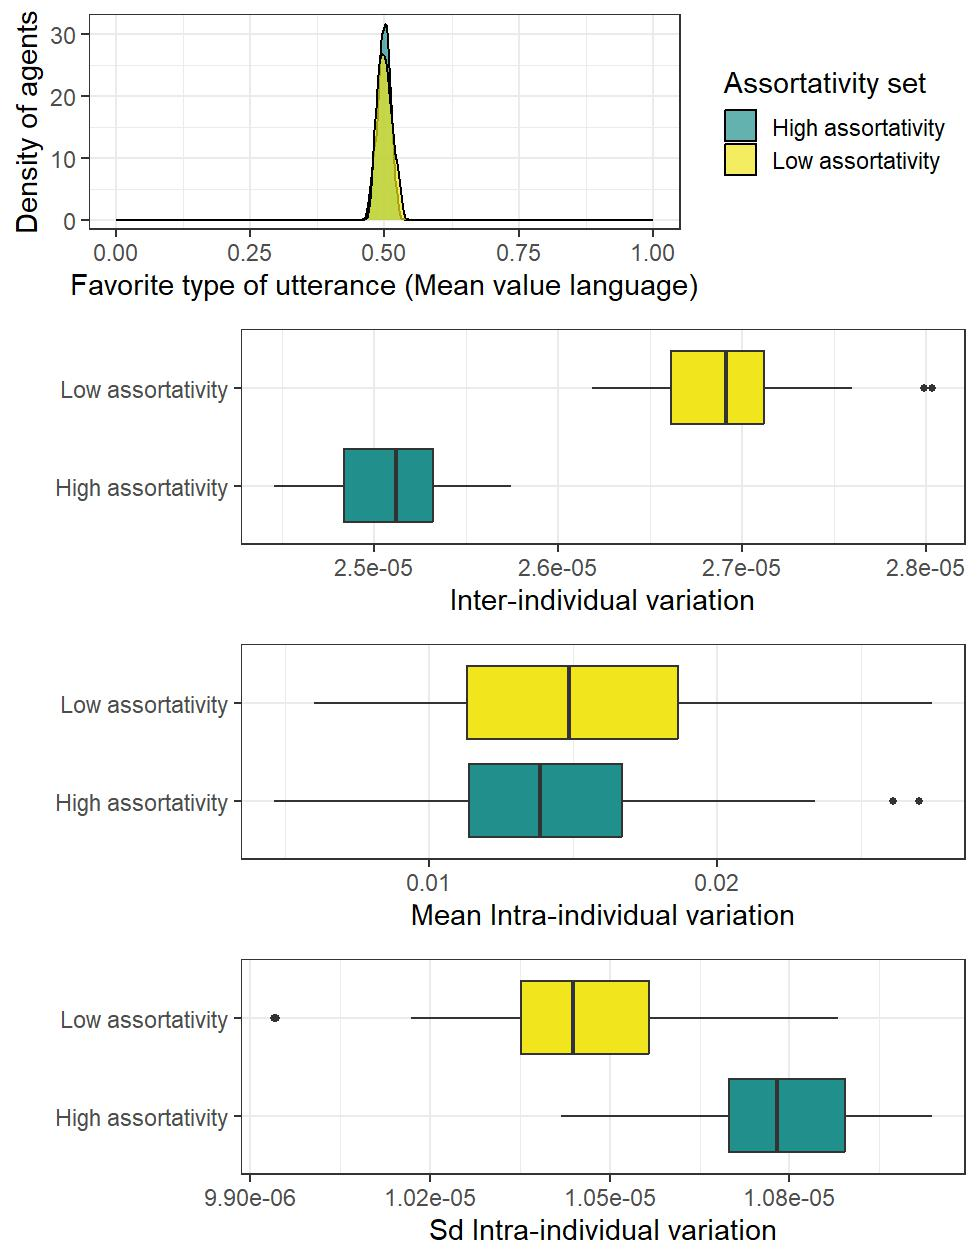
\includegraphics{./Figures/unnamed-chunk-44-1} 

}

\caption{Looking at the variability inter- and intra-individual in sets varying in *assortativity* in network with a continuous language. The first graph shows the value of the language: it shows the favorite utterance for each agents in the three types of population (variable initial language exposure). The second graph shows the  inter-individual variation (the x scale is the average Kullback-Leibler divergence on all pairs of agents). The third and fourth graph show respectively the mean and standard deviation on the intra-individual variation for all agents (the x scale shows respectively the mean and the std of the entropy on the Dirichlet internal representation of agents). In all the following graphs, green shows high value in the metrics while yellow shows low value in the metric.}\label{fig:unnamed-chunk-44}
\end{figure}

Here, we want to understand whether the effect size under these
differences is high or low.

We apply Cohen's d test and a classic t.test, in networks
\textbf{without} language exposure, \textbf{with (weak)} language
exposure, and \textbf{with (strong)} language exposure. We gathered the
results in a summary table:

COhen's \emph{D}:

\begin{longtable}[]{@{}
  >{\raggedright\arraybackslash}p{(\columnwidth - 12\tabcolsep) * \real{0.1972}}
  >{\raggedright\arraybackslash}p{(\columnwidth - 12\tabcolsep) * \real{0.1972}}
  >{\raggedright\arraybackslash}p{(\columnwidth - 12\tabcolsep) * \real{0.1690}}
  >{\raggedleft\arraybackslash}p{(\columnwidth - 12\tabcolsep) * \real{0.0986}}
  >{\raggedright\arraybackslash}p{(\columnwidth - 12\tabcolsep) * \real{0.1408}}
  >{\raggedleft\arraybackslash}p{(\columnwidth - 12\tabcolsep) * \real{0.0986}}
  >{\raggedleft\arraybackslash}p{(\columnwidth - 12\tabcolsep) * \real{0.0986}}@{}}
\toprule()
\begin{minipage}[b]{\linewidth}\raggedright
Measure
\end{minipage} & \begin{minipage}[b]{\linewidth}\raggedright
TypeVariation
\end{minipage} & \begin{minipage}[b]{\linewidth}\raggedright
TypeLangage
\end{minipage} & \begin{minipage}[b]{\linewidth}\raggedleft
CohenD
\end{minipage} & \begin{minipage}[b]{\linewidth}\raggedright
Magnitude
\end{minipage} & \begin{minipage}[b]{\linewidth}\raggedleft
CI\_Inf
\end{minipage} & \begin{minipage}[b]{\linewidth}\raggedleft
CI\_Sup
\end{minipage} \\
\midrule()
\endhead
assortativity & Inter & None & 5.139 & large & 5.717 & 4.561 \\
assortativity & Mean Intra & None & 0.232 & small & 0.512 & 0.048 \\
assortativity & Std Intra & None & 2.174 & large & 1.822 & 2.526 \\
\bottomrule()
\end{longtable}

\emph{T}-Test:

\begin{longtable}[]{@{}
  >{\raggedright\arraybackslash}p{(\columnwidth - 14\tabcolsep) * \real{0.1750}}
  >{\raggedright\arraybackslash}p{(\columnwidth - 14\tabcolsep) * \real{0.1750}}
  >{\raggedright\arraybackslash}p{(\columnwidth - 14\tabcolsep) * \real{0.1500}}
  >{\raggedleft\arraybackslash}p{(\columnwidth - 14\tabcolsep) * \real{0.1000}}
  >{\raggedleft\arraybackslash}p{(\columnwidth - 14\tabcolsep) * \real{0.1000}}
  >{\raggedleft\arraybackslash}p{(\columnwidth - 14\tabcolsep) * \real{0.1250}}
  >{\raggedleft\arraybackslash}p{(\columnwidth - 14\tabcolsep) * \real{0.0875}}
  >{\raggedleft\arraybackslash}p{(\columnwidth - 14\tabcolsep) * \real{0.0875}}@{}}
\toprule()
\begin{minipage}[b]{\linewidth}\raggedright
Measure
\end{minipage} & \begin{minipage}[b]{\linewidth}\raggedright
TypeVariation
\end{minipage} & \begin{minipage}[b]{\linewidth}\raggedright
TypeLangage
\end{minipage} & \begin{minipage}[b]{\linewidth}\raggedleft
T\_value
\end{minipage} & \begin{minipage}[b]{\linewidth}\raggedleft
DF
\end{minipage} & \begin{minipage}[b]{\linewidth}\raggedleft
PValue
\end{minipage} & \begin{minipage}[b]{\linewidth}\raggedleft
CI\_Inf
\end{minipage} & \begin{minipage}[b]{\linewidth}\raggedleft
CI\_Sup
\end{minipage} \\
\midrule()
\endhead
assortativity & Inter & None & -36.338 & 188.901 & 0.0000000 & 0.000 &
0 \\
assortativity & Mean Intra & None & -1.643 & 190.737 & 0.1021278 & 0.003
& 0 \\
assortativity & Std Intra & None & 15.373 & 192.193 & 0.0000000 & 0.000
& 0 \\
\bottomrule()
\end{longtable}

\hypertarget{exponent-1}{%
\paragraph{Exponent}\label{exponent-1}}

These sets of networks were obtained using \textbf{scale-free} networks.

We first observe the values of the two sets:

\begin{longtable}[]{@{}
  >{\raggedright\arraybackslash}p{(\columnwidth - 14\tabcolsep) * \real{0.1978}}
  >{\raggedleft\arraybackslash}p{(\columnwidth - 14\tabcolsep) * \real{0.1209}}
  >{\raggedleft\arraybackslash}p{(\columnwidth - 14\tabcolsep) * \real{0.1099}}
  >{\raggedleft\arraybackslash}p{(\columnwidth - 14\tabcolsep) * \real{0.1209}}
  >{\raggedleft\arraybackslash}p{(\columnwidth - 14\tabcolsep) * \real{0.1538}}
  >{\raggedleft\arraybackslash}p{(\columnwidth - 14\tabcolsep) * \real{0.0989}}
  >{\raggedleft\arraybackslash}p{(\columnwidth - 14\tabcolsep) * \real{0.0549}}
  >{\raggedright\arraybackslash}p{(\columnwidth - 14\tabcolsep) * \real{0.1429}}@{}}
\toprule()
\begin{minipage}[b]{\linewidth}\raggedright
\end{minipage} & \begin{minipage}[b]{\linewidth}\raggedleft
pathlength
\end{minipage} & \begin{minipage}[b]{\linewidth}\raggedleft
neighbors
\end{minipage} & \begin{minipage}[b]{\linewidth}\raggedleft
clustering
\end{minipage} & \begin{minipage}[b]{\linewidth}\raggedleft
assortativity
\end{minipage} & \begin{minipage}[b]{\linewidth}\raggedleft
exponent
\end{minipage} & \begin{minipage}[b]{\linewidth}\raggedleft
size
\end{minipage} & \begin{minipage}[b]{\linewidth}\raggedright
network\_type
\end{minipage} \\
\midrule()
\endhead
Low exponent set & 4.003612 & 2 & 0 & -0.2662336 & 2.610069 & 50 &
Scalefree \\
High exponent set & 3.988955 & 2 & 0 & -0.2615309 & 3.067970 & 50 &
Scalefree \\
\bottomrule()
\end{longtable}

This should be interpreted in the following way:

\begin{itemize}
\tightlist
\item
  there is a difference of 0.4579 between the two sets concerning
  \emph{exponent}
\item
  there are differences of 0 for the \emph{neighbors}, 0 for the
  \emph{clustering} coefficient, -0.0147 for the \emph{pathlength},
  0.0047 for the \emph{assortativity}, and 0 for the \emph{size}
\end{itemize}

Thus, we compare the differences in inter and intra-individual variation
between the two sets. We believe that these differences will reflect the
differences in exponent, as the other metrics are kept (almost)
constant.

We look at the differences between the two sets:

\begin{figure}[!H]

{\centering 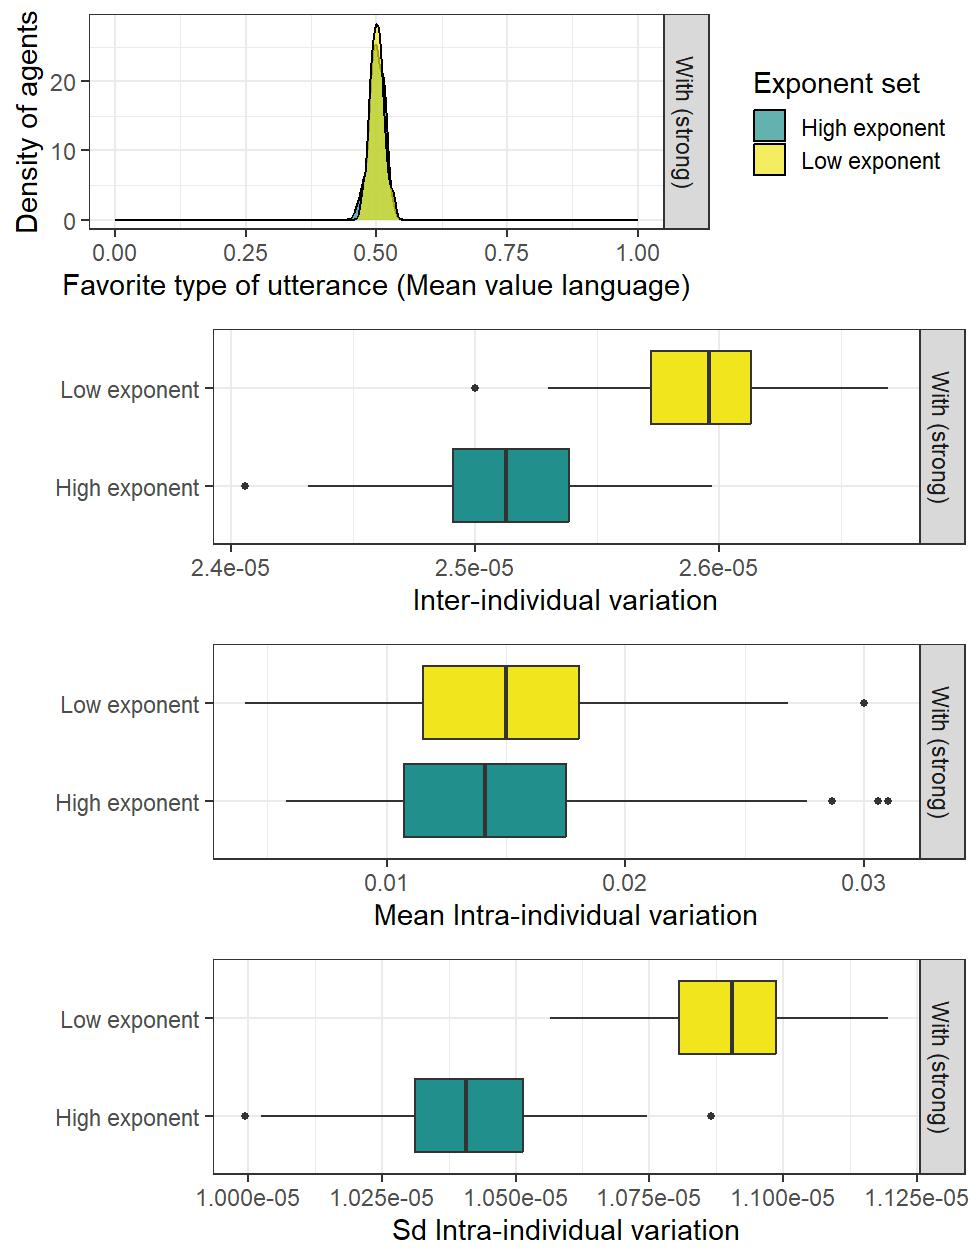
\includegraphics{./Figures/unnamed-chunk-48-1} 

}

\caption{Looking at the variability inter- and intra-individual in sets varying in *exponent* in network with a continuous language. The first graph shows the value of the language: it shows the favorite utterance for each agents in the three types of population (variable initial language exposure). The second graph shows the  inter-individual variation (the x scale is the average Kullback-Leibler divergence on all pairs of agents). The third and fourth graph show respectively the mean and standard deviation on the intra-individual variation for all agents (the x scale shows respectively the mean and the std of the entropy on the Dirichlet internal representation of agents). In all the following graphs, green shows high value in the metrics while yellow shows low value in the metric.}\label{fig:unnamed-chunk-48}
\end{figure}

Here, we want to understand whether the effect size under these
differences is high or low.

We apply Cohen's d test and a classic t.test, in networks
\textbf{without} language exposure, \textbf{with (weak)} language
exposure, and \textbf{with (strong)} language exposure. We gathered the
results in a summary table:

Cohen's \emph{D}:

\begin{longtable}[]{@{}
  >{\raggedright\arraybackslash}p{(\columnwidth - 12\tabcolsep) * \real{0.1343}}
  >{\raggedright\arraybackslash}p{(\columnwidth - 12\tabcolsep) * \real{0.2090}}
  >{\raggedright\arraybackslash}p{(\columnwidth - 12\tabcolsep) * \real{0.1791}}
  >{\raggedleft\arraybackslash}p{(\columnwidth - 12\tabcolsep) * \real{0.1045}}
  >{\raggedright\arraybackslash}p{(\columnwidth - 12\tabcolsep) * \real{0.1642}}
  >{\raggedleft\arraybackslash}p{(\columnwidth - 12\tabcolsep) * \real{0.1045}}
  >{\raggedleft\arraybackslash}p{(\columnwidth - 12\tabcolsep) * \real{0.1045}}@{}}
\toprule()
\begin{minipage}[b]{\linewidth}\raggedright
Measure
\end{minipage} & \begin{minipage}[b]{\linewidth}\raggedright
TypeVariation
\end{minipage} & \begin{minipage}[b]{\linewidth}\raggedright
TypeLangage
\end{minipage} & \begin{minipage}[b]{\linewidth}\raggedleft
CohenD
\end{minipage} & \begin{minipage}[b]{\linewidth}\raggedright
Magnitude
\end{minipage} & \begin{minipage}[b]{\linewidth}\raggedleft
CI\_Inf
\end{minipage} & \begin{minipage}[b]{\linewidth}\raggedleft
CI\_Sup
\end{minipage} \\
\midrule()
\endhead
exponent & Inter & None & 2.357 & large & 2.720 & 1.994 \\
exponent & Mean Intra & None & 0.033 & negligible & 0.312 & 0.246 \\
exponent & Std Intra & None & 3.359 & large & 3.792 & 2.926 \\
\bottomrule()
\end{longtable}

\emph{T}-Test:

\begin{longtable}[]{@{}
  >{\raggedright\arraybackslash}p{(\columnwidth - 14\tabcolsep) * \real{0.1200}}
  >{\raggedright\arraybackslash}p{(\columnwidth - 14\tabcolsep) * \real{0.1867}}
  >{\raggedright\arraybackslash}p{(\columnwidth - 14\tabcolsep) * \real{0.1600}}
  >{\raggedleft\arraybackslash}p{(\columnwidth - 14\tabcolsep) * \real{0.1067}}
  >{\raggedleft\arraybackslash}p{(\columnwidth - 14\tabcolsep) * \real{0.1067}}
  >{\raggedleft\arraybackslash}p{(\columnwidth - 14\tabcolsep) * \real{0.1333}}
  >{\raggedleft\arraybackslash}p{(\columnwidth - 14\tabcolsep) * \real{0.0933}}
  >{\raggedleft\arraybackslash}p{(\columnwidth - 14\tabcolsep) * \real{0.0933}}@{}}
\toprule()
\begin{minipage}[b]{\linewidth}\raggedright
Measure
\end{minipage} & \begin{minipage}[b]{\linewidth}\raggedright
TypeVariation
\end{minipage} & \begin{minipage}[b]{\linewidth}\raggedright
TypeLangage
\end{minipage} & \begin{minipage}[b]{\linewidth}\raggedleft
T\_value
\end{minipage} & \begin{minipage}[b]{\linewidth}\raggedleft
DF
\end{minipage} & \begin{minipage}[b]{\linewidth}\raggedleft
PValue
\end{minipage} & \begin{minipage}[b]{\linewidth}\raggedleft
CI\_Inf
\end{minipage} & \begin{minipage}[b]{\linewidth}\raggedleft
CI\_Sup
\end{minipage} \\
\midrule()
\endhead
exponent & Inter & None & -16.667 & 190.982 & 0.0000000 & 0.000 &
0.000 \\
exponent & Mean Intra & None & -0.233 & 197.326 & 0.8157111 & 0.002 &
0.001 \\
exponent & Std Intra & None & -23.753 & 176.871 & 0.0000000 & 0.000 &
0.000 \\
\bottomrule()
\end{longtable}

\hypertarget{size-1}{%
\paragraph{Size}\label{size-1}}

These sets of networks were obtained using \textbf{scale-free} networks.

We first observe the values of the two sets:

\begin{longtable}[]{@{}
  >{\raggedright\arraybackslash}p{(\columnwidth - 14\tabcolsep) * \real{0.1609}}
  >{\raggedleft\arraybackslash}p{(\columnwidth - 14\tabcolsep) * \real{0.1264}}
  >{\raggedleft\arraybackslash}p{(\columnwidth - 14\tabcolsep) * \real{0.1149}}
  >{\raggedleft\arraybackslash}p{(\columnwidth - 14\tabcolsep) * \real{0.1264}}
  >{\raggedleft\arraybackslash}p{(\columnwidth - 14\tabcolsep) * \real{0.1609}}
  >{\raggedleft\arraybackslash}p{(\columnwidth - 14\tabcolsep) * \real{0.1034}}
  >{\raggedleft\arraybackslash}p{(\columnwidth - 14\tabcolsep) * \real{0.0575}}
  >{\raggedright\arraybackslash}p{(\columnwidth - 14\tabcolsep) * \real{0.1494}}@{}}
\toprule()
\begin{minipage}[b]{\linewidth}\raggedright
\end{minipage} & \begin{minipage}[b]{\linewidth}\raggedleft
pathlength
\end{minipage} & \begin{minipage}[b]{\linewidth}\raggedleft
neighbors
\end{minipage} & \begin{minipage}[b]{\linewidth}\raggedleft
clustering
\end{minipage} & \begin{minipage}[b]{\linewidth}\raggedleft
assortativity
\end{minipage} & \begin{minipage}[b]{\linewidth}\raggedleft
exponent
\end{minipage} & \begin{minipage}[b]{\linewidth}\raggedleft
size
\end{minipage} & \begin{minipage}[b]{\linewidth}\raggedright
network\_type
\end{minipage} \\
\midrule()
\endhead
Low size set & 4.428812 & 2 & 0 & -0.2983585 & 2.845419 & 50 &
Scalefree \\
High size set & 4.439875 & 2 & 0 & -0.2902309 & 2.854948 & 100 &
Scalefree \\
\bottomrule()
\end{longtable}

This should be interpreted in the following way:

\begin{itemize}
\tightlist
\item
  there is a difference of 50 between the two sets concerning
  \emph{size}
\item
  there are differences of 0 for the \emph{neighbors}, 0 for the
  \emph{clustering} coefficient, 0.0111 for the \emph{pathlength},
  0.0081 for the \emph{assortativity}, and 0.0095 for the
  \emph{exponent}
\end{itemize}

Thus, we compare the differences in inter and intra-individual variation
between the two sets. We believe that these differences will reflect the
differences in size, as the other metrics are kept (almost) constant.

We look at the differences between the two sets:

\begin{figure}[!H]

{\centering 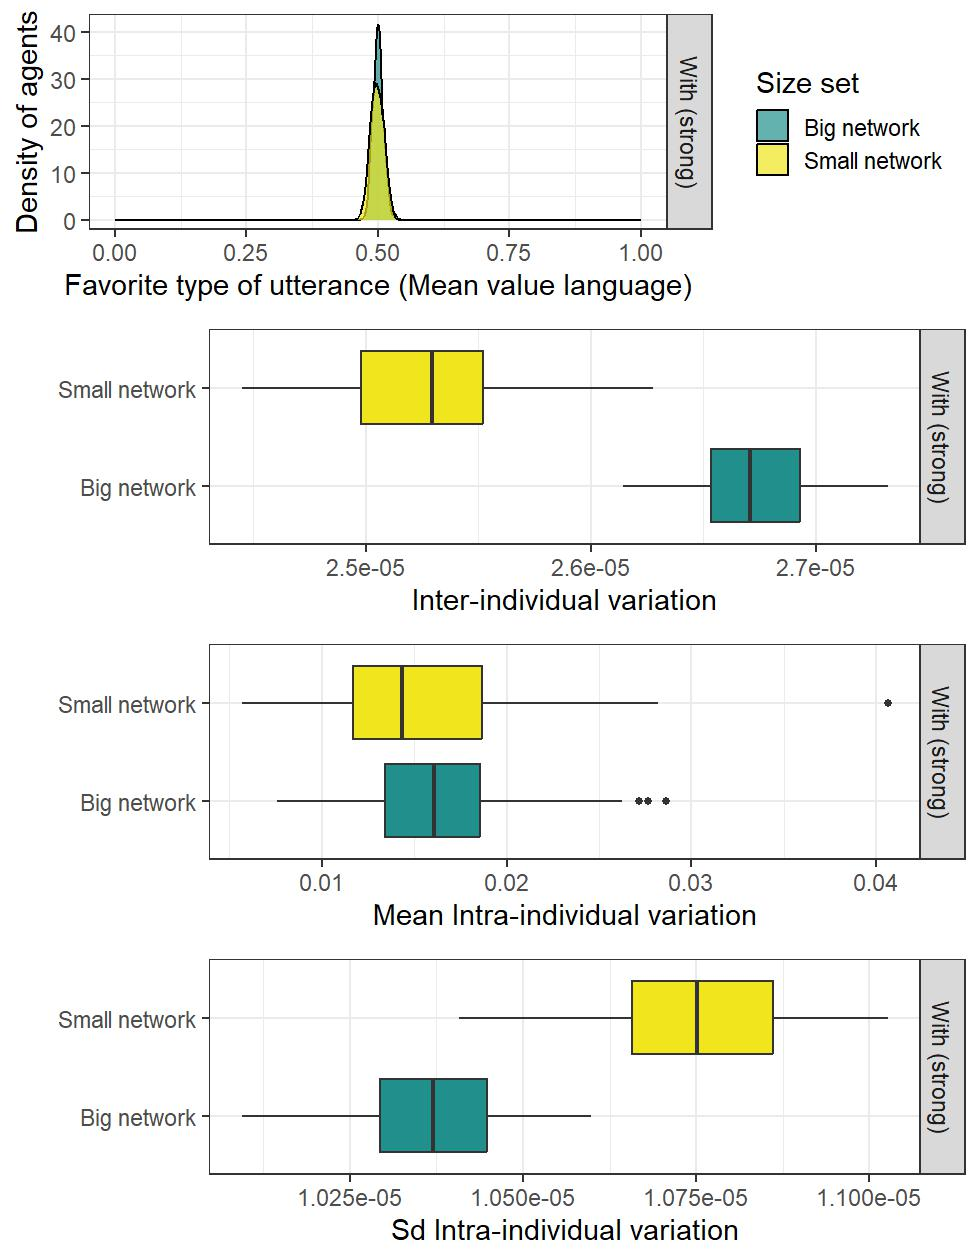
\includegraphics{./Figures/unnamed-chunk-52-1} 

}

\caption{Looking at the variability inter- and intra-individual in sets varying in *size* in network with a continuous language. The first graph shows the value of the language: it shows the favorite utterance for each agents in the three types of population (variable initial language exposure). The second graph shows the  inter-individual variation (the x scale is the average Kullback-Leibler divergence on all pairs of agents). The third and fourth graph show respectively the mean and standard deviation on the intra-individual variation for all agents (the x scale shows respectively the mean and the std of the entropy on the Dirichlet internal representation of agents). In all the following graphs, green shows high value in the metrics while yellow shows low value in the metric.}\label{fig:unnamed-chunk-52}
\end{figure}

Here, we want to understand whether the effect size under these
differences is high or low.

We apply Cohen's d test and a classic t.test, in networks
\textbf{without} language exposure, \textbf{with (weak)} language
exposure, and \textbf{with (strong)} language exposure. We gathered the
results in a summary table:

Cohen's \emph{D}:

\begin{longtable}[]{@{}
  >{\raggedright\arraybackslash}p{(\columnwidth - 12\tabcolsep) * \real{0.1231}}
  >{\raggedright\arraybackslash}p{(\columnwidth - 12\tabcolsep) * \real{0.2154}}
  >{\raggedright\arraybackslash}p{(\columnwidth - 12\tabcolsep) * \real{0.1846}}
  >{\raggedleft\arraybackslash}p{(\columnwidth - 12\tabcolsep) * \real{0.1077}}
  >{\raggedright\arraybackslash}p{(\columnwidth - 12\tabcolsep) * \real{0.1538}}
  >{\raggedleft\arraybackslash}p{(\columnwidth - 12\tabcolsep) * \real{0.1077}}
  >{\raggedleft\arraybackslash}p{(\columnwidth - 12\tabcolsep) * \real{0.1077}}@{}}
\toprule()
\begin{minipage}[b]{\linewidth}\raggedright
Measure
\end{minipage} & \begin{minipage}[b]{\linewidth}\raggedright
TypeVariation
\end{minipage} & \begin{minipage}[b]{\linewidth}\raggedright
TypeLangage
\end{minipage} & \begin{minipage}[b]{\linewidth}\raggedleft
CohenD
\end{minipage} & \begin{minipage}[b]{\linewidth}\raggedright
Magnitude
\end{minipage} & \begin{minipage}[b]{\linewidth}\raggedleft
CI\_Inf
\end{minipage} & \begin{minipage}[b]{\linewidth}\raggedleft
CI\_Sup
\end{minipage} \\
\midrule()
\endhead
size & Inter & None & 4.608 & large & 4.075 & 5.141 \\
size & Mean Intra & None & 0.213 & small & 0.067 & 0.493 \\
size & Std Intra & None & 2.871 & large & 3.269 & 2.474 \\
\bottomrule()
\end{longtable}

\emph{T}-Test:

\begin{longtable}[]{@{}
  >{\raggedright\arraybackslash}p{(\columnwidth - 14\tabcolsep) * \real{0.1081}}
  >{\raggedright\arraybackslash}p{(\columnwidth - 14\tabcolsep) * \real{0.1892}}
  >{\raggedright\arraybackslash}p{(\columnwidth - 14\tabcolsep) * \real{0.1622}}
  >{\raggedleft\arraybackslash}p{(\columnwidth - 14\tabcolsep) * \real{0.1081}}
  >{\raggedleft\arraybackslash}p{(\columnwidth - 14\tabcolsep) * \real{0.1081}}
  >{\raggedleft\arraybackslash}p{(\columnwidth - 14\tabcolsep) * \real{0.1351}}
  >{\raggedleft\arraybackslash}p{(\columnwidth - 14\tabcolsep) * \real{0.0946}}
  >{\raggedleft\arraybackslash}p{(\columnwidth - 14\tabcolsep) * \real{0.0946}}@{}}
\toprule()
\begin{minipage}[b]{\linewidth}\raggedright
Measure
\end{minipage} & \begin{minipage}[b]{\linewidth}\raggedright
TypeVariation
\end{minipage} & \begin{minipage}[b]{\linewidth}\raggedright
TypeLangage
\end{minipage} & \begin{minipage}[b]{\linewidth}\raggedleft
T\_value
\end{minipage} & \begin{minipage}[b]{\linewidth}\raggedleft
DF
\end{minipage} & \begin{minipage}[b]{\linewidth}\raggedleft
PValue
\end{minipage} & \begin{minipage}[b]{\linewidth}\raggedleft
CI\_Inf
\end{minipage} & \begin{minipage}[b]{\linewidth}\raggedleft
CI\_Sup
\end{minipage} \\
\midrule()
\endhead
size & Inter & None & 32.586 & 177.690 & 0.0000000 & 0 & 0.000 \\
size & Mean Intra & None & 1.505 & 187.882 & 0.1339995 & 0 & 0.003 \\
size & Std Intra & None & -20.304 & 189.611 & 0.0000000 & 0 & 0.000 \\
\bottomrule()
\end{longtable}

\hypertarget{clustering-coefficient-1}{%
\paragraph{Clustering coefficient}\label{clustering-coefficient-1}}

These sets of networks were obtained using \textbf{small-world}
networks, and varying the parameters \texttt{rewire}.

We first observe the values of the two sets:

\begin{longtable}[]{@{}
  >{\raggedright\arraybackslash}p{(\columnwidth - 14\tabcolsep) * \real{0.2151}}
  >{\raggedleft\arraybackslash}p{(\columnwidth - 14\tabcolsep) * \real{0.1183}}
  >{\raggedleft\arraybackslash}p{(\columnwidth - 14\tabcolsep) * \real{0.1075}}
  >{\raggedleft\arraybackslash}p{(\columnwidth - 14\tabcolsep) * \real{0.1183}}
  >{\raggedleft\arraybackslash}p{(\columnwidth - 14\tabcolsep) * \real{0.1505}}
  >{\raggedleft\arraybackslash}p{(\columnwidth - 14\tabcolsep) * \real{0.0968}}
  >{\raggedleft\arraybackslash}p{(\columnwidth - 14\tabcolsep) * \real{0.0538}}
  >{\raggedright\arraybackslash}p{(\columnwidth - 14\tabcolsep) * \real{0.1398}}@{}}
\toprule()
\begin{minipage}[b]{\linewidth}\raggedright
\end{minipage} & \begin{minipage}[b]{\linewidth}\raggedleft
pathlength
\end{minipage} & \begin{minipage}[b]{\linewidth}\raggedleft
neighbors
\end{minipage} & \begin{minipage}[b]{\linewidth}\raggedleft
clustering
\end{minipage} & \begin{minipage}[b]{\linewidth}\raggedleft
assortativity
\end{minipage} & \begin{minipage}[b]{\linewidth}\raggedleft
exponent
\end{minipage} & \begin{minipage}[b]{\linewidth}\raggedleft
size
\end{minipage} & \begin{minipage}[b]{\linewidth}\raggedright
network\_type
\end{minipage} \\
\midrule()
\endhead
Low clustering set & 1.677852 & 48 & 0.3191316 & -0.0151775 & NA & 150 &
Small-world \\
High clustering set & 1.682726 & 48 & 0.5820881 & -0.0041973 & NA & 150
& Small-world \\
\bottomrule()
\end{longtable}

This should be interpreted in the following way:

\begin{itemize}
\tightlist
\item
  there is a difference of NA between the two sets concerning
  \emph{clustering} coefficient
\item
  there are differences of NA for the \emph{neighbors}, NA for the
  \emph{pathlength} coefficient, NA for the \emph{assortativity}, NA for
  the \emph{exponent}, and NA for the \emph{size}
\end{itemize}

Thus, we compare the differences in inter and intra-individual variation
between the two sets. We believe that these differences will reflect the
differences in clustering, as the other metrics are kept (almost)
constant.

We look at the differences between the two sets:

\begin{figure}[!H]

{\centering 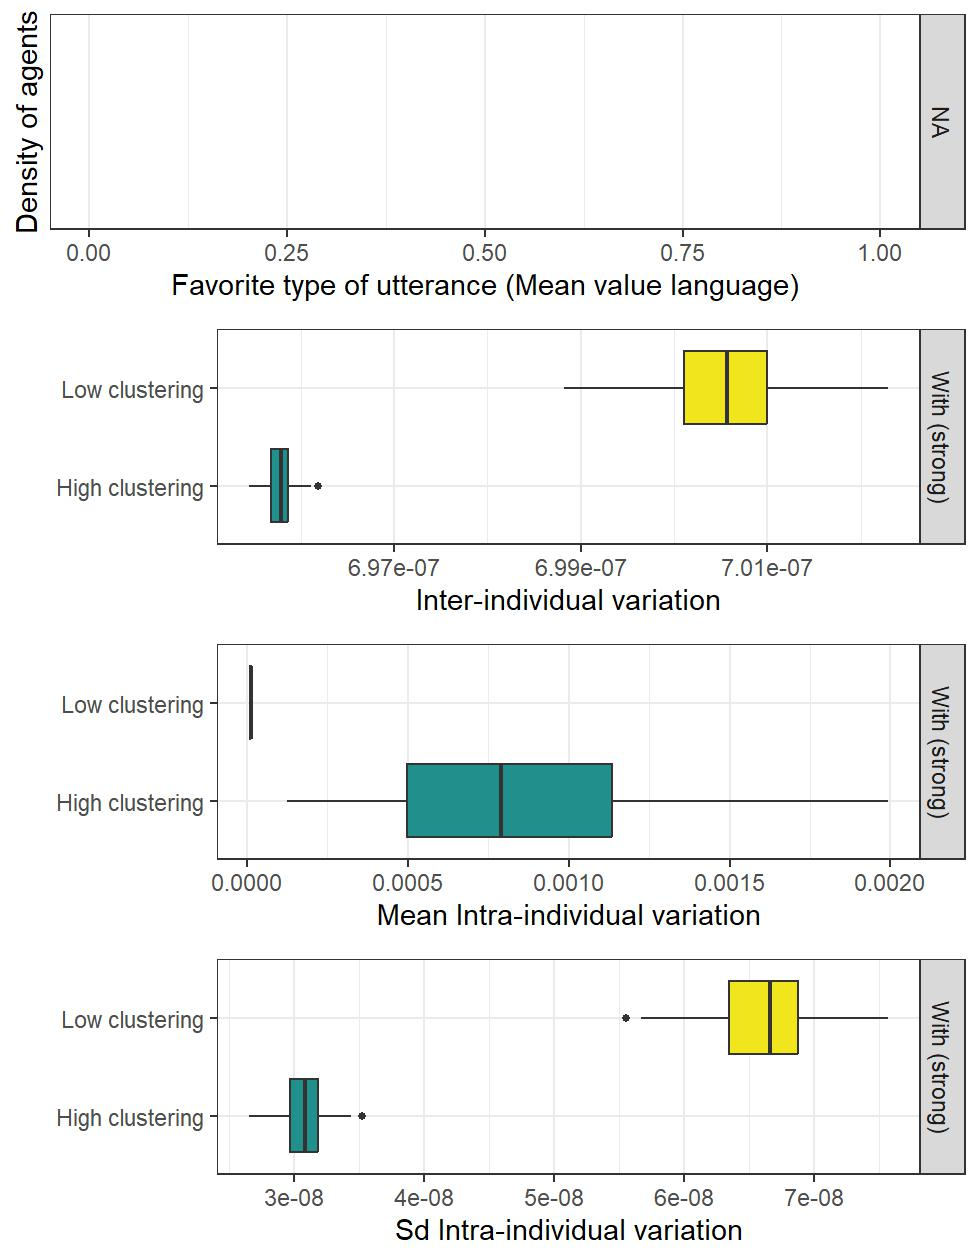
\includegraphics{./Figures/unnamed-chunk-57-1} 

}

\caption{Looking at the variability inter- and intra-individual in sets varying in *clustering coefficient* in network with a continuous language. The first graph shows the value of the language: it shows the favorite utterance for each agents in the three types of population (variable initial language exposure). The second graph shows the  inter-individual variation (the x scale is the average Kullback-Leibler divergence on all pairs of agents). The third and fourth graph show respectively the mean and standard deviation on the intra-individual variation for all agents (the x scale shows respectively the mean and the std of the entropy on the Dirichlet internal representation of agents). In all the following graphs, green shows high value in the metrics while yellow shows low value in the metric.}\label{fig:unnamed-chunk-57}
\end{figure}

Please note that the \texttt{x} scale here is different due to
differences in the network type.

Here, we want to understand whether the effect size under these
differences is high or low.

We apply Cohen's d test and a classic t.test, in networks
\textbf{without} language exposure, \textbf{with (weak)} language
exposure, and \textbf{with (strong)} language exposure. We gathered the
results in a summary table:

Cohen's \emph{D}:

\begin{longtable}[]{@{}
  >{\raggedright\arraybackslash}p{(\columnwidth - 12\tabcolsep) * \real{0.1618}}
  >{\raggedright\arraybackslash}p{(\columnwidth - 12\tabcolsep) * \real{0.2059}}
  >{\raggedright\arraybackslash}p{(\columnwidth - 12\tabcolsep) * \real{0.1765}}
  >{\raggedleft\arraybackslash}p{(\columnwidth - 12\tabcolsep) * \real{0.1029}}
  >{\raggedright\arraybackslash}p{(\columnwidth - 12\tabcolsep) * \real{0.1471}}
  >{\raggedleft\arraybackslash}p{(\columnwidth - 12\tabcolsep) * \real{0.1029}}
  >{\raggedleft\arraybackslash}p{(\columnwidth - 12\tabcolsep) * \real{0.1029}}@{}}
\toprule()
\begin{minipage}[b]{\linewidth}\raggedright
Measure
\end{minipage} & \begin{minipage}[b]{\linewidth}\raggedright
TypeVariation
\end{minipage} & \begin{minipage}[b]{\linewidth}\raggedright
TypeLangage
\end{minipage} & \begin{minipage}[b]{\linewidth}\raggedleft
CohenD
\end{minipage} & \begin{minipage}[b]{\linewidth}\raggedright
Magnitude
\end{minipage} & \begin{minipage}[b]{\linewidth}\raggedleft
CI\_Inf
\end{minipage} & \begin{minipage}[b]{\linewidth}\raggedleft
CI\_Sup
\end{minipage} \\
\midrule()
\endhead
clustering & Inter & None & 9.538 & large & 10.519 & 8.557 \\
clustering & Mean Intra & None & 2.721 & large & 2.334 & 3.108 \\
clustering & Std Intra & None & 11.598 & large & 12.775 & 10.421 \\
\bottomrule()
\end{longtable}

\emph{T}-Test:

\begin{longtable}[]{@{}
  >{\raggedright\arraybackslash}p{(\columnwidth - 14\tabcolsep) * \real{0.1486}}
  >{\raggedright\arraybackslash}p{(\columnwidth - 14\tabcolsep) * \real{0.1892}}
  >{\raggedright\arraybackslash}p{(\columnwidth - 14\tabcolsep) * \real{0.1622}}
  >{\raggedleft\arraybackslash}p{(\columnwidth - 14\tabcolsep) * \real{0.1081}}
  >{\raggedleft\arraybackslash}p{(\columnwidth - 14\tabcolsep) * \real{0.1081}}
  >{\raggedleft\arraybackslash}p{(\columnwidth - 14\tabcolsep) * \real{0.0946}}
  >{\raggedleft\arraybackslash}p{(\columnwidth - 14\tabcolsep) * \real{0.0946}}
  >{\raggedleft\arraybackslash}p{(\columnwidth - 14\tabcolsep) * \real{0.0946}}@{}}
\toprule()
\begin{minipage}[b]{\linewidth}\raggedright
Measure
\end{minipage} & \begin{minipage}[b]{\linewidth}\raggedright
TypeVariation
\end{minipage} & \begin{minipage}[b]{\linewidth}\raggedright
TypeLangage
\end{minipage} & \begin{minipage}[b]{\linewidth}\raggedleft
T\_value
\end{minipage} & \begin{minipage}[b]{\linewidth}\raggedleft
DF
\end{minipage} & \begin{minipage}[b]{\linewidth}\raggedleft
PValue
\end{minipage} & \begin{minipage}[b]{\linewidth}\raggedleft
CI\_Inf
\end{minipage} & \begin{minipage}[b]{\linewidth}\raggedleft
CI\_Sup
\end{minipage} \\
\midrule()
\endhead
clustering & Inter & None & -67.443 & 109.604 & 0 & 0.000 & 0.000 \\
clustering & Mean Intra & None & 19.242 & 99.004 & 0 & 0.001 & 0.001 \\
clustering & Std Intra & None & -82.009 & 141.684 & 0 & 0.000 & 0.000 \\
\bottomrule()
\end{longtable}

\hypertarget{node-degree-1}{%
\paragraph{Node degree}\label{node-degree-1}}

These sets of networks were obtained using \textbf{random} networks.

We first observe the values of the two sets:

\begin{longtable}[]{@{}
  >{\raggedright\arraybackslash}p{(\columnwidth - 14\tabcolsep) * \real{0.2234}}
  >{\raggedleft\arraybackslash}p{(\columnwidth - 14\tabcolsep) * \real{0.1170}}
  >{\raggedleft\arraybackslash}p{(\columnwidth - 14\tabcolsep) * \real{0.1064}}
  >{\raggedleft\arraybackslash}p{(\columnwidth - 14\tabcolsep) * \real{0.1170}}
  >{\raggedleft\arraybackslash}p{(\columnwidth - 14\tabcolsep) * \real{0.1489}}
  >{\raggedleft\arraybackslash}p{(\columnwidth - 14\tabcolsep) * \real{0.0957}}
  >{\raggedleft\arraybackslash}p{(\columnwidth - 14\tabcolsep) * \real{0.0532}}
  >{\raggedright\arraybackslash}p{(\columnwidth - 14\tabcolsep) * \real{0.1383}}@{}}
\toprule()
\begin{minipage}[b]{\linewidth}\raggedright
\end{minipage} & \begin{minipage}[b]{\linewidth}\raggedleft
pathlength
\end{minipage} & \begin{minipage}[b]{\linewidth}\raggedleft
neighbors
\end{minipage} & \begin{minipage}[b]{\linewidth}\raggedleft
clustering
\end{minipage} & \begin{minipage}[b]{\linewidth}\raggedleft
assortativity
\end{minipage} & \begin{minipage}[b]{\linewidth}\raggedleft
exponent
\end{minipage} & \begin{minipage}[b]{\linewidth}\raggedleft
size
\end{minipage} & \begin{minipage}[b]{\linewidth}\raggedright
network\_type
\end{minipage} \\
\midrule()
\endhead
Low node degree set & 1.785351 & 12.0072 & 0.244033 & 0.0116981 & NA &
50 & Random \\
High node degree set & 1.785351 & 12.0072 & 0.244033 & 0.0116981 & NA &
50 & Random \\
\bottomrule()
\end{longtable}

This should be interpreted in the following way:

\begin{itemize}
\tightlist
\item
  there is a difference of -0.0032 between the two sets concerning
  \emph{node degree}
\item
  there are differences of 0.0024 for the \emph{clustering} coefficient,
  0.1377 for the \emph{pathlength} coefficient, 0.0021 for the
  \emph{assortativity}, NA for the \emph{exponent}, and 0 for the
  \emph{size}
\end{itemize}

Thus, we compare the differences in inter and intra-individual variation
between the two sets. We believe that these differences will reflect the
differences in node degree, as the other metrics are kept (almost)
constant.

We look at the differences between the two sets:

\begin{figure}[!H]

{\centering 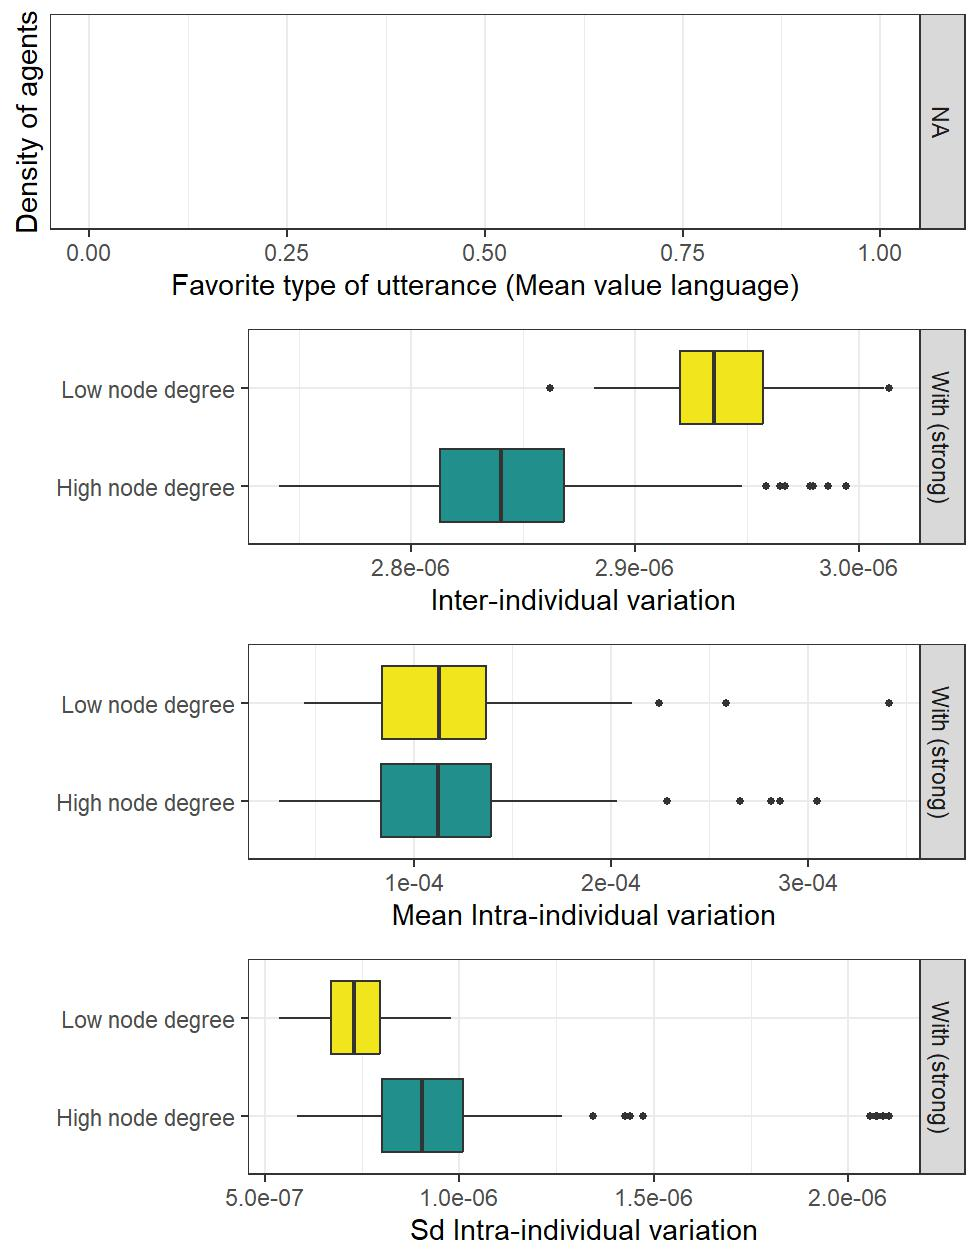
\includegraphics{./Figures/unnamed-chunk-62-1} 

}

\caption{Looking at the variability inter- and intra-individual in sets varying in *node degree* in network with a continuous language. The first graph shows the value of the language: it shows the favorite utterance for each agents in the three types of population (variable initial language exposure). The second graph shows the  inter-individual variation (the x scale is the average Kullback-Leibler divergence on all pairs of agents). The third and fourth graph show respectively the mean and standard deviation on the intra-individual variation for all agents (the x scale shows respectively the mean and the std of the entropy on the Dirichlet internal representation of agents). In all the following graphs, green shows high value in the metrics while yellow shows low value in the metric.}\label{fig:unnamed-chunk-62}
\end{figure}

Please note that the \texttt{x} scale here is different due to
differences in the network type.

Here, we want to understand whether the effect size under these
differences is high or low.

We apply Cohen's d test and a classic t.test, in networks
\textbf{without} language exposure, \textbf{with (weak)} language
exposure, and \textbf{with (strong)} language exposure. We gathered the
results in a summary table:

Cohen's \emph{D}:

\begin{longtable}[]{@{}
  >{\raggedright\arraybackslash}p{(\columnwidth - 12\tabcolsep) * \real{0.1714}}
  >{\raggedright\arraybackslash}p{(\columnwidth - 12\tabcolsep) * \real{0.2000}}
  >{\raggedright\arraybackslash}p{(\columnwidth - 12\tabcolsep) * \real{0.1714}}
  >{\raggedleft\arraybackslash}p{(\columnwidth - 12\tabcolsep) * \real{0.1000}}
  >{\raggedright\arraybackslash}p{(\columnwidth - 12\tabcolsep) * \real{0.1571}}
  >{\raggedleft\arraybackslash}p{(\columnwidth - 12\tabcolsep) * \real{0.1000}}
  >{\raggedleft\arraybackslash}p{(\columnwidth - 12\tabcolsep) * \real{0.1000}}@{}}
\toprule()
\begin{minipage}[b]{\linewidth}\raggedright
Measure
\end{minipage} & \begin{minipage}[b]{\linewidth}\raggedright
TypeVariation
\end{minipage} & \begin{minipage}[b]{\linewidth}\raggedright
TypeLangage
\end{minipage} & \begin{minipage}[b]{\linewidth}\raggedleft
CohenD
\end{minipage} & \begin{minipage}[b]{\linewidth}\raggedright
Magnitude
\end{minipage} & \begin{minipage}[b]{\linewidth}\raggedleft
CI\_Inf
\end{minipage} & \begin{minipage}[b]{\linewidth}\raggedleft
CI\_Sup
\end{minipage} \\
\midrule()
\endhead
node\_degree & Inter & None & 2.183 & large & 2.535 & 1.830 \\
node\_degree & Mean Intra & None & 0.038 & negligible & 0.240 & 0.317 \\
node\_degree & Std Intra & None & 0.981 & large & 0.686 & 1.277 \\
\bottomrule()
\end{longtable}

\emph{T}-Test:

\begin{longtable}[]{@{}
  >{\raggedright\arraybackslash}p{(\columnwidth - 14\tabcolsep) * \real{0.1538}}
  >{\raggedright\arraybackslash}p{(\columnwidth - 14\tabcolsep) * \real{0.1795}}
  >{\raggedright\arraybackslash}p{(\columnwidth - 14\tabcolsep) * \real{0.1538}}
  >{\raggedleft\arraybackslash}p{(\columnwidth - 14\tabcolsep) * \real{0.1026}}
  >{\raggedleft\arraybackslash}p{(\columnwidth - 14\tabcolsep) * \real{0.1026}}
  >{\raggedleft\arraybackslash}p{(\columnwidth - 14\tabcolsep) * \real{0.1282}}
  >{\raggedleft\arraybackslash}p{(\columnwidth - 14\tabcolsep) * \real{0.0897}}
  >{\raggedleft\arraybackslash}p{(\columnwidth - 14\tabcolsep) * \real{0.0897}}@{}}
\toprule()
\begin{minipage}[b]{\linewidth}\raggedright
Measure
\end{minipage} & \begin{minipage}[b]{\linewidth}\raggedright
TypeVariation
\end{minipage} & \begin{minipage}[b]{\linewidth}\raggedright
TypeLangage
\end{minipage} & \begin{minipage}[b]{\linewidth}\raggedleft
T\_value
\end{minipage} & \begin{minipage}[b]{\linewidth}\raggedleft
DF
\end{minipage} & \begin{minipage}[b]{\linewidth}\raggedleft
PValue
\end{minipage} & \begin{minipage}[b]{\linewidth}\raggedleft
CI\_Inf
\end{minipage} & \begin{minipage}[b]{\linewidth}\raggedleft
CI\_Sup
\end{minipage} \\
\midrule()
\endhead
node\_degree & Inter & None & -15.433 & 159.110 & 0.0000000 & 0 & 0 \\
node\_degree & Mean Intra & None & 0.272 & 196.039 & 0.7860134 & 0 &
0 \\
node\_degree & Std Intra & None & 6.939 & 116.802 & 0.0000000 & 0 & 0 \\
\bottomrule()
\end{longtable}

\hypertarget{pathlength-using-random-1}{%
\paragraph{Pathlength (using random)}\label{pathlength-using-random-1}}

These sets of networks were obtained using \textbf{random} networks.
Pathlength was already explored using \emph{scale-free} networks, and
controlling for many metrics. Here, we just want to observe the effect
of \emph{pathlength} in opposite to the effect of \emph{mean degree}, in
random network.

We first observe the values of the two sets:

\begin{longtable}[]{@{}
  >{\raggedright\arraybackslash}p{(\columnwidth - 14\tabcolsep) * \real{0.2151}}
  >{\raggedleft\arraybackslash}p{(\columnwidth - 14\tabcolsep) * \real{0.1183}}
  >{\raggedleft\arraybackslash}p{(\columnwidth - 14\tabcolsep) * \real{0.1075}}
  >{\raggedleft\arraybackslash}p{(\columnwidth - 14\tabcolsep) * \real{0.1183}}
  >{\raggedleft\arraybackslash}p{(\columnwidth - 14\tabcolsep) * \real{0.1505}}
  >{\raggedleft\arraybackslash}p{(\columnwidth - 14\tabcolsep) * \real{0.0968}}
  >{\raggedleft\arraybackslash}p{(\columnwidth - 14\tabcolsep) * \real{0.0538}}
  >{\raggedright\arraybackslash}p{(\columnwidth - 14\tabcolsep) * \real{0.1398}}@{}}
\toprule()
\begin{minipage}[b]{\linewidth}\raggedright
\end{minipage} & \begin{minipage}[b]{\linewidth}\raggedleft
pathlength
\end{minipage} & \begin{minipage}[b]{\linewidth}\raggedleft
neighbors
\end{minipage} & \begin{minipage}[b]{\linewidth}\raggedleft
clustering
\end{minipage} & \begin{minipage}[b]{\linewidth}\raggedleft
assortativity
\end{minipage} & \begin{minipage}[b]{\linewidth}\raggedleft
exponent
\end{minipage} & \begin{minipage}[b]{\linewidth}\raggedleft
size
\end{minipage} & \begin{minipage}[b]{\linewidth}\raggedright
network\_type
\end{minipage} \\
\midrule()
\endhead
Low pathlength set & 4.461143 & 2.4594 & 0.0323188 & -0.0946811 & NA &
50 & Random \\
High pathlength set & 4.461143 & 2.4594 & 0.0323188 & -0.0946811 & NA &
50 & Random \\
\bottomrule()
\end{longtable}

This should be interpreted in the following way:

\begin{itemize}
\tightlist
\item
  there is a difference of 0.1377 between the two sets concerning
  \emph{pathlength}
\item
  there are differences of 0.0024 for the \emph{clustering} coefficient,
  -0.0032 for the \emph{node degree} coefficient, 0.0021 for the
  \emph{assortativity}, NA for the \emph{exponent}, and 0 for the
  \emph{size}
\end{itemize}

Thus, we compare the differences in inter and intra-individual variation
between the two sets. We believe that these differences will reflect the
differences in node degree, as the other metrics are kept (almost)
constant.

We look at the differences between the two sets:

\begin{figure}[!H]

{\centering 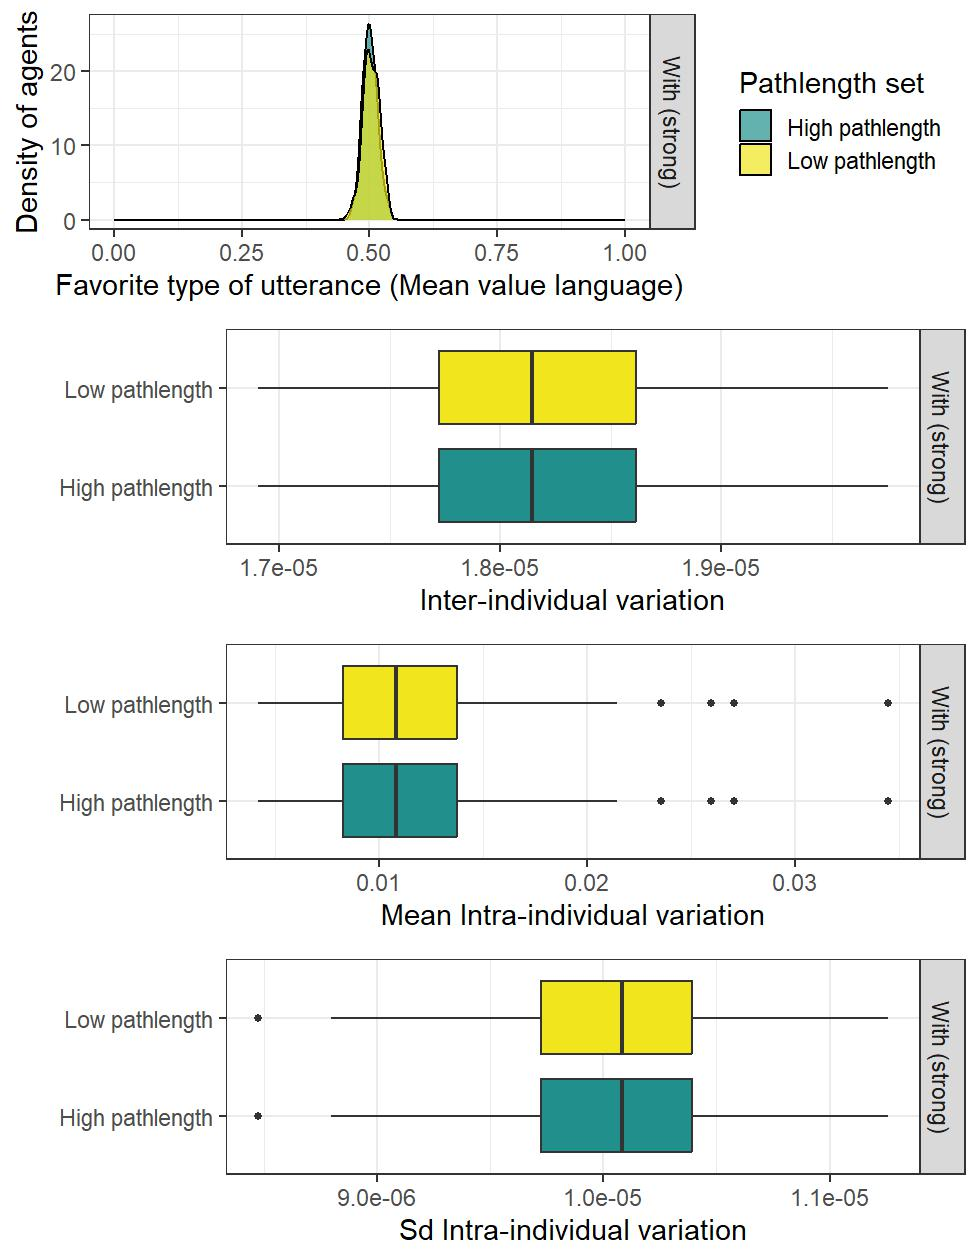
\includegraphics{./Figures/unnamed-chunk-66-1} 

}

\caption{Looking at the variability inter- and intra-individual in sets varying in *pathlength* in network with a continuous language. The first graph shows the value of the language: it shows the favorite utterance for each agents in the three types of population (variable initial language exposure). The second graph shows the  inter-individual variation (the x scale is the average Kullback-Leibler divergence on all pairs of agents). The third and fourth graph show respectively the mean and standard deviation on the intra-individual variation for all agents (the x scale shows respectively the mean and the std of the entropy on the Dirichlet internal representation of agents). In all the following graphs, green shows high value in the metrics while yellow shows low value in the metric.}\label{fig:unnamed-chunk-66}
\end{figure}

Please note that the \texttt{x} scale here is different due to
differences in the network type.

Here, we want to understand whether the effect size under these
differences is high or low.

We apply Cohen's d test and a classic t.test, in networks
\textbf{without} language exposure, \textbf{with (weak)} language
exposure, and \textbf{with (strong)} language exposure. We gathered the
results in a summary table:

COhen's \emph{D}:

\begin{longtable}[]{@{}
  >{\raggedright\arraybackslash}p{(\columnwidth - 12\tabcolsep) * \real{0.2055}}
  >{\raggedright\arraybackslash}p{(\columnwidth - 12\tabcolsep) * \real{0.1918}}
  >{\raggedright\arraybackslash}p{(\columnwidth - 12\tabcolsep) * \real{0.1644}}
  >{\raggedleft\arraybackslash}p{(\columnwidth - 12\tabcolsep) * \real{0.0959}}
  >{\raggedright\arraybackslash}p{(\columnwidth - 12\tabcolsep) * \real{0.1507}}
  >{\raggedleft\arraybackslash}p{(\columnwidth - 12\tabcolsep) * \real{0.0959}}
  >{\raggedleft\arraybackslash}p{(\columnwidth - 12\tabcolsep) * \real{0.0959}}@{}}
\toprule()
\begin{minipage}[b]{\linewidth}\raggedright
Measure
\end{minipage} & \begin{minipage}[b]{\linewidth}\raggedright
TypeVariation
\end{minipage} & \begin{minipage}[b]{\linewidth}\raggedright
TypeLangage
\end{minipage} & \begin{minipage}[b]{\linewidth}\raggedleft
CohenD
\end{minipage} & \begin{minipage}[b]{\linewidth}\raggedright
Magnitude
\end{minipage} & \begin{minipage}[b]{\linewidth}\raggedleft
CI\_Inf
\end{minipage} & \begin{minipage}[b]{\linewidth}\raggedleft
CI\_Sup
\end{minipage} \\
\midrule()
\endhead
pathlength\_ran & Inter & None & 0 & negligible & 0.279 & 0.279 \\
pathlength\_ran & Mean Intra & None & 0 & negligible & 0.279 & 0.279 \\
pathlength\_ran & Std Intra & None & 0 & negligible & 0.279 & 0.279 \\
\bottomrule()
\end{longtable}

\emph{T}-Test:

\begin{longtable}[]{@{}
  >{\raggedright\arraybackslash}p{(\columnwidth - 14\tabcolsep) * \real{0.2027}}
  >{\raggedright\arraybackslash}p{(\columnwidth - 14\tabcolsep) * \real{0.1892}}
  >{\raggedright\arraybackslash}p{(\columnwidth - 14\tabcolsep) * \real{0.1622}}
  >{\raggedleft\arraybackslash}p{(\columnwidth - 14\tabcolsep) * \real{0.1081}}
  >{\raggedleft\arraybackslash}p{(\columnwidth - 14\tabcolsep) * \real{0.0541}}
  >{\raggedleft\arraybackslash}p{(\columnwidth - 14\tabcolsep) * \real{0.0946}}
  >{\raggedleft\arraybackslash}p{(\columnwidth - 14\tabcolsep) * \real{0.0946}}
  >{\raggedleft\arraybackslash}p{(\columnwidth - 14\tabcolsep) * \real{0.0946}}@{}}
\toprule()
\begin{minipage}[b]{\linewidth}\raggedright
Measure
\end{minipage} & \begin{minipage}[b]{\linewidth}\raggedright
TypeVariation
\end{minipage} & \begin{minipage}[b]{\linewidth}\raggedright
TypeLangage
\end{minipage} & \begin{minipage}[b]{\linewidth}\raggedleft
T\_value
\end{minipage} & \begin{minipage}[b]{\linewidth}\raggedleft
DF
\end{minipage} & \begin{minipage}[b]{\linewidth}\raggedleft
PValue
\end{minipage} & \begin{minipage}[b]{\linewidth}\raggedleft
CI\_Inf
\end{minipage} & \begin{minipage}[b]{\linewidth}\raggedleft
CI\_Sup
\end{minipage} \\
\midrule()
\endhead
pathlength\_ran & Inter & None & 0 & 198 & 1 & 0.000 & 0.000 \\
pathlength\_ran & Mean Intra & None & 0 & 198 & 1 & 0.001 & 0.001 \\
pathlength\_ran & Std Intra & None & 0 & 198 & 1 & 0.000 & 0.000 \\
\bottomrule()
\end{longtable}

\hypertarget{summary-continuous}{%
\paragraph{Summary continuous}\label{summary-continuous}}

\begin{center}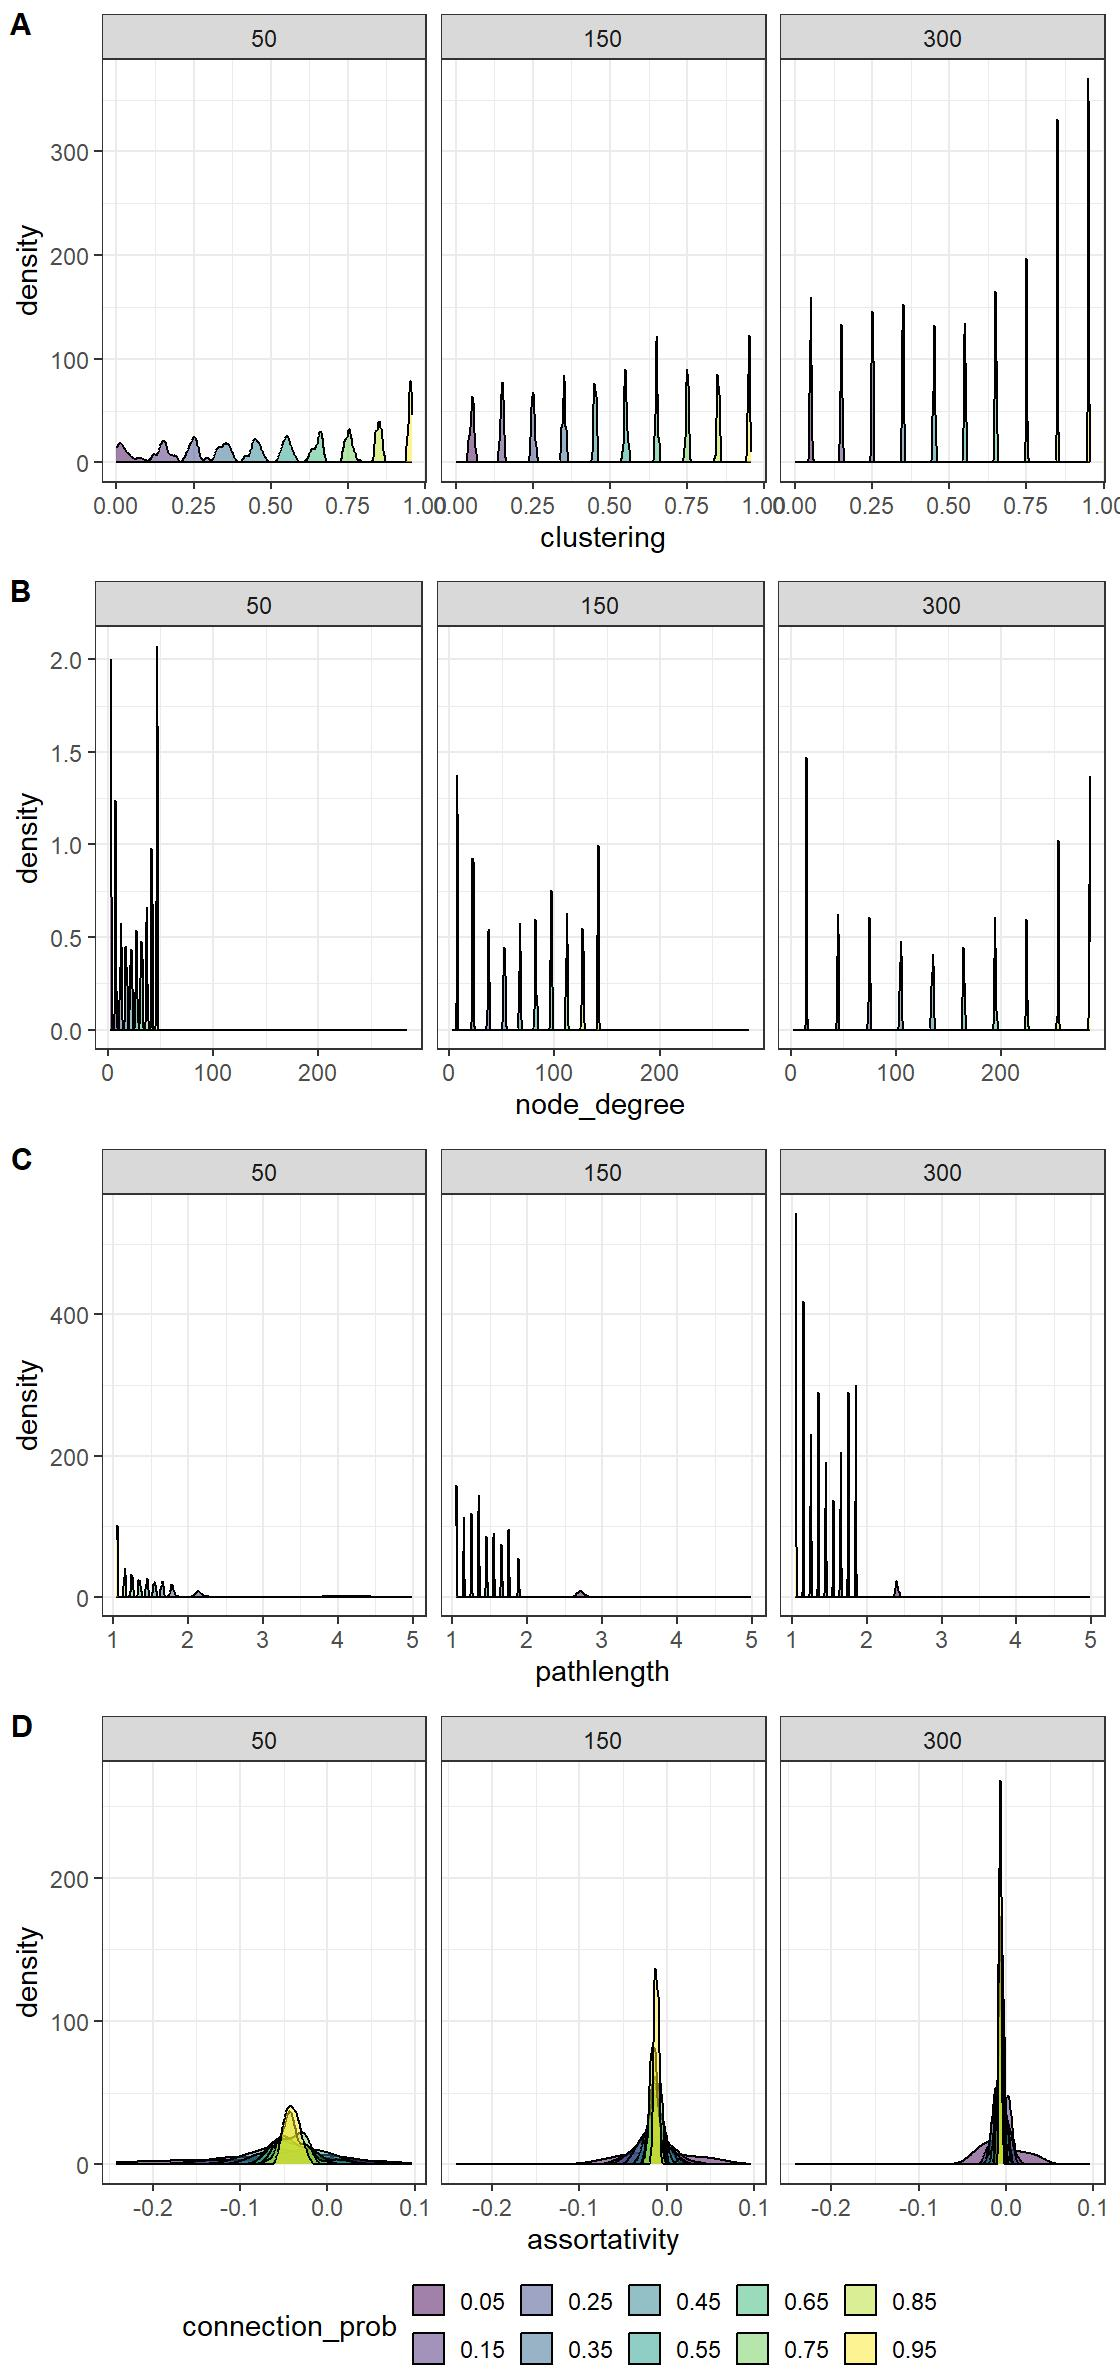
\includegraphics{./Figures/unnamed-chunk-69-1} \end{center}

\hypertarget{dataset-2-looking-at-correlations-and-models}{%
\subsection{DATASET 2: looking at correlations and
models}\label{dataset-2-looking-at-correlations-and-models}}

In this dataset, we generated thousands of simulations using
\emph{random}, \emph{small-world} and \emph{scalefree} networks. Using
this dataset, we aim to:

\begin{itemize}
\tightlist
\item
  look at the correlations between our metrics
\item
  investigate the relative strength of each metric using models
\end{itemize}

While in dataset 1 we use specific sets of networks (which can be seen
as ``unnatural''), in Dataset 2, we observe ``natural'' networks
(namely, we did not choose to exclude any of the networks generated).
Also, here we only analyzed a \emph{multinomial} language (no data from
networks with continuous language, contrary to Dataset 1). You can refer
to \protect\hyperlink{parameters}{Parameters} to know more about the
parameters which were investigated, but please note that a summary (and
data distribution) of the results is also presented below.

\hypertarget{data-distribution}{%
\subsubsection{Data distribution}\label{data-distribution}}

Please note that \emph{exponent} is a metric considered only in
scale-free networks. Additionnally, \emph{node degree} and
\emph{clustering coefficient} are considered only in small-world and
random network, since they do not vary in scale-free networks. We look
at the data for each network type.

\textbf{Random networks}

\begin{longtable}[]{@{}
  >{\raggedright\arraybackslash}p{(\columnwidth - 20\tabcolsep) * \real{0.0188}}
  >{\raggedright\arraybackslash}p{(\columnwidth - 20\tabcolsep) * \real{0.0500}}
  >{\raggedright\arraybackslash}p{(\columnwidth - 20\tabcolsep) * \real{0.0938}}
  >{\raggedright\arraybackslash}p{(\columnwidth - 20\tabcolsep) * \real{0.0938}}
  >{\raggedright\arraybackslash}p{(\columnwidth - 20\tabcolsep) * \real{0.0875}}
  >{\raggedright\arraybackslash}p{(\columnwidth - 20\tabcolsep) * \real{0.1125}}
  >{\raggedright\arraybackslash}p{(\columnwidth - 20\tabcolsep) * \real{0.1250}}
  >{\raggedright\arraybackslash}p{(\columnwidth - 20\tabcolsep) * \real{0.1000}}
  >{\raggedright\arraybackslash}p{(\columnwidth - 20\tabcolsep) * \real{0.1125}}
  >{\raggedright\arraybackslash}p{(\columnwidth - 20\tabcolsep) * \real{0.0938}}
  >{\raggedright\arraybackslash}p{(\columnwidth - 20\tabcolsep) * \real{0.1125}}@{}}
\toprule()
\begin{minipage}[b]{\linewidth}\raggedright
\end{minipage} & \begin{minipage}[b]{\linewidth}\raggedright
size
\end{minipage} & \begin{minipage}[b]{\linewidth}\raggedright
clustering
\end{minipage} & \begin{minipage}[b]{\linewidth}\raggedright
node\_degree
\end{minipage} & \begin{minipage}[b]{\linewidth}\raggedright
pathlength
\end{minipage} & \begin{minipage}[b]{\linewidth}\raggedright
assortativity
\end{minipage} & \begin{minipage}[b]{\linewidth}\raggedright
init\_lang\_exp
\end{minipage} & \begin{minipage}[b]{\linewidth}\raggedright
connection\_prob
\end{minipage} & \begin{minipage}[b]{\linewidth}\raggedright
inter\_var
\end{minipage} & \begin{minipage}[b]{\linewidth}\raggedright
mean\_intra\_var
\end{minipage} & \begin{minipage}[b]{\linewidth}\raggedright
std\_intra\_var
\end{minipage} \\
\midrule()
\endhead
& 50 :300 & Min. :0.0000 & Min. : 2.20 & Min. :1.043 & Min. :-0.241523 &
With (strong):298 & Min. :0.0500 & Min. :6.300e-08 & Min. :0.7455 & Min.
:3.542e-05 \\
& 150:295 & 1st Qu.:0.2506 & 1st Qu.: 22.71 & 1st Qu.:1.250 & 1st
Qu.:-0.031982 & With (weak) :298 & 1st Qu.:0.2500 & 1st Qu.:1.264e-06 &
1st Qu.:1.3053 & 1st Qu.:5.088e-04 \\
& 300:300 & Median :0.5294 & Median : 51.09 & Median :1.469 & Median
:-0.013001 & Without :299 & Median :0.5500 & Median :4.474e-06 & Median
:1.9657 & Median :1.192e-03 \\
& NA & Mean :0.5010 & Mean : 83.12 & Mean :1.620 & Mean :-0.021829 & NA
& Mean :0.5015 & Mean :3.374e-04 & Mean :1.8145 & Mean :3.937e-03 \\
& NA & 3rd Qu.:0.7495 & 3rd Qu.:126.51 & 3rd Qu.:1.751 & 3rd
Qu.:-0.005664 & NA & 3rd Qu.:0.7500 & 3rd Qu.:1.702e-05 & 3rd Qu.:2.2386
& 3rd Qu.:2.611e-03 \\
& NA & Max. :0.9568 & Max. :284.75 & Max. :4.985 & Max. : 0.096417 & NA
& Max. :0.9500 & Max. :1.957e-02 & Max. :2.3002 & Max. :1.242e-01 \\
\bottomrule()
\end{longtable}

Quick note: the number of random network is not exactly equal to 900
because we removed a few networks where there were isolated components.

In random networks, the only structural parameters we manipulated were
the \emph{connection probability} (from 0.05 to 0.95 in steps of 0.05)
and the \emph{size} (50, 150, and 300).

\begin{figure}[!H]

{\centering 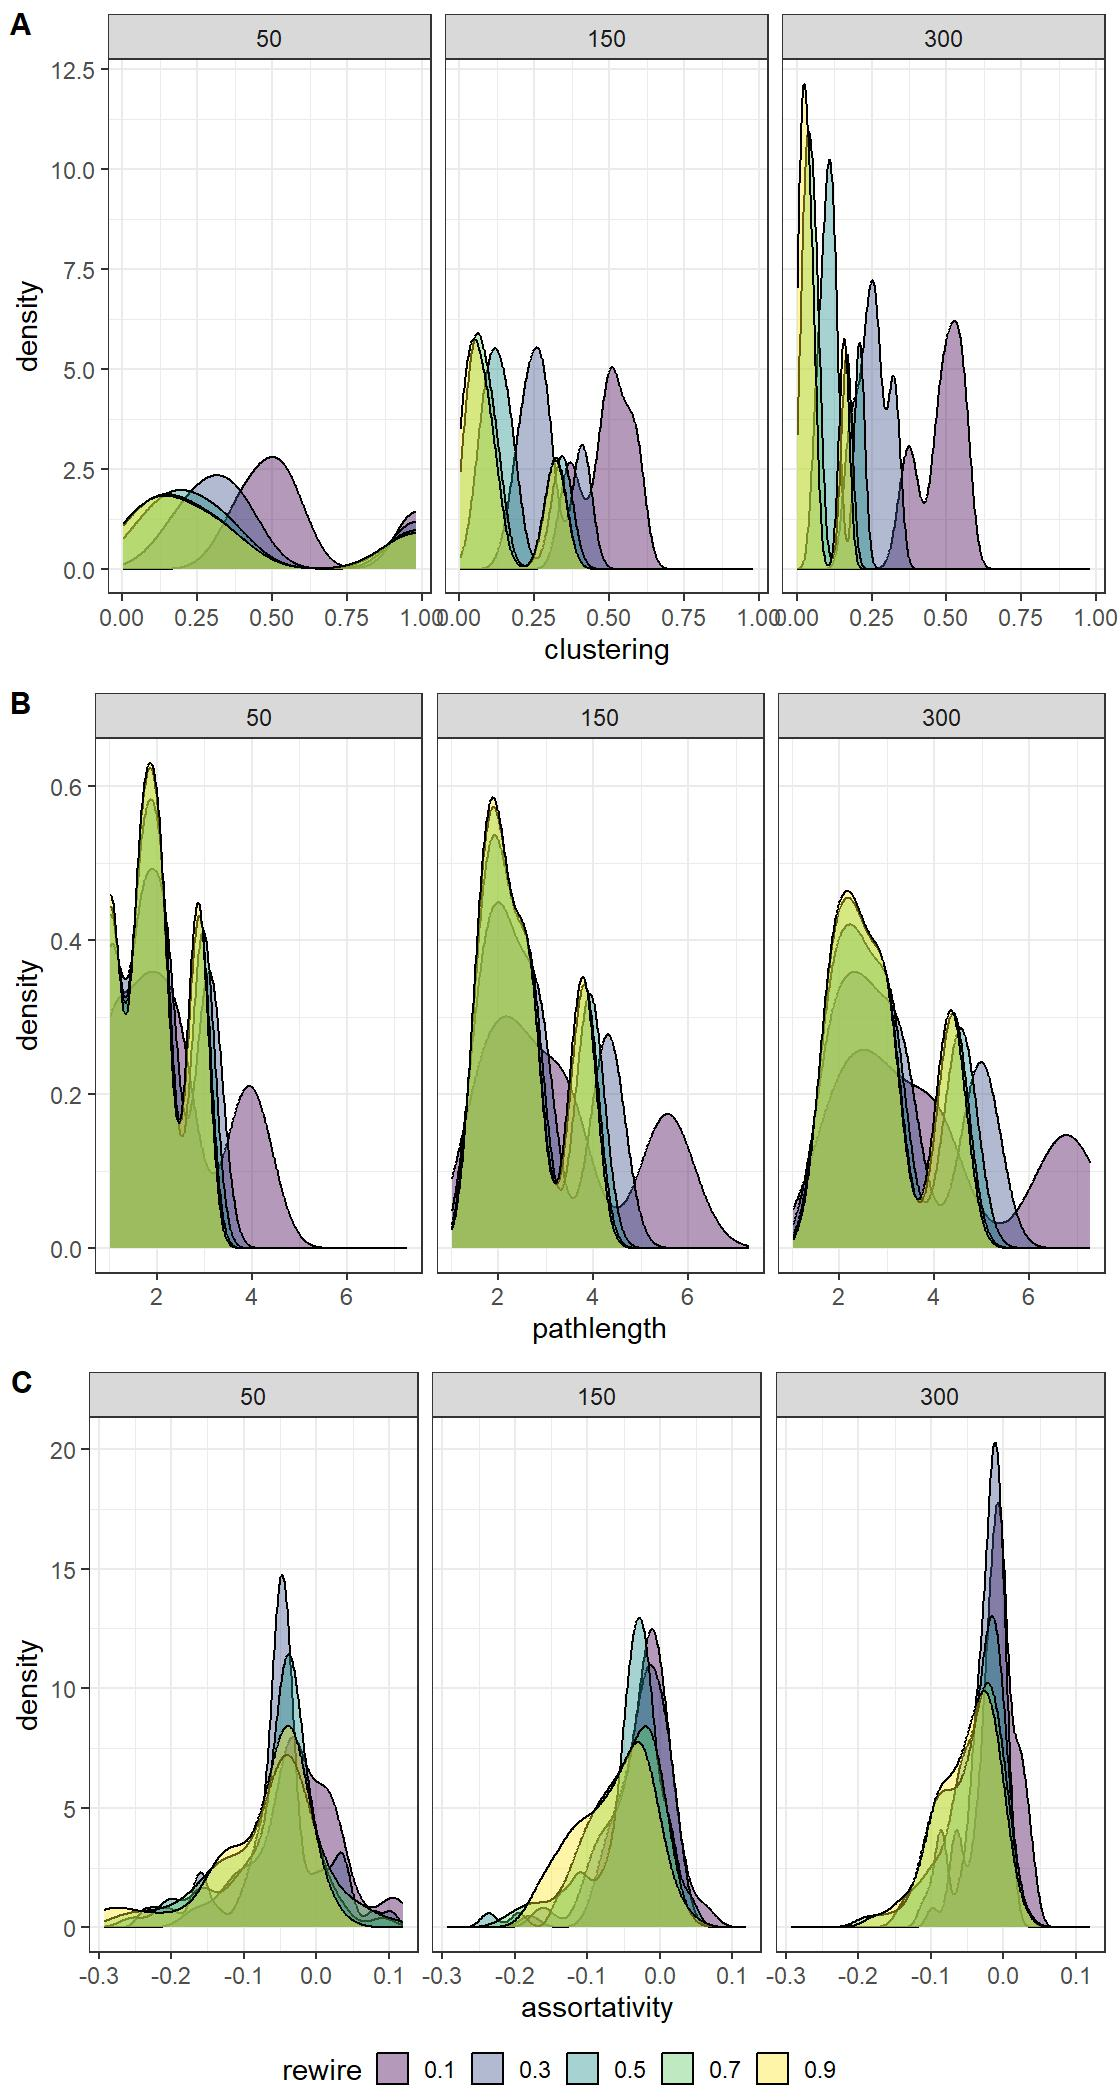
\includegraphics{./Figures/unnamed-chunk-73-1} 

}

\caption{Distribution of the data in random networks.}\label{fig:unnamed-chunk-73}
\end{figure}

\textbf{Scale-free networks}

\begin{longtable}[]{@{}
  >{\raggedright\arraybackslash}p{(\columnwidth - 16\tabcolsep) * \real{0.0244}}
  >{\raggedright\arraybackslash}p{(\columnwidth - 16\tabcolsep) * \real{0.0650}}
  >{\raggedright\arraybackslash}p{(\columnwidth - 16\tabcolsep) * \real{0.1138}}
  >{\raggedright\arraybackslash}p{(\columnwidth - 16\tabcolsep) * \real{0.1138}}
  >{\raggedright\arraybackslash}p{(\columnwidth - 16\tabcolsep) * \real{0.1301}}
  >{\raggedright\arraybackslash}p{(\columnwidth - 16\tabcolsep) * \real{0.1626}}
  >{\raggedright\arraybackslash}p{(\columnwidth - 16\tabcolsep) * \real{0.1382}}
  >{\raggedright\arraybackslash}p{(\columnwidth - 16\tabcolsep) * \real{0.1220}}
  >{\raggedright\arraybackslash}p{(\columnwidth - 16\tabcolsep) * \real{0.1301}}@{}}
\toprule()
\begin{minipage}[b]{\linewidth}\raggedright
\end{minipage} & \begin{minipage}[b]{\linewidth}\raggedright
size
\end{minipage} & \begin{minipage}[b]{\linewidth}\raggedright
exponent
\end{minipage} & \begin{minipage}[b]{\linewidth}\raggedright
pathlength
\end{minipage} & \begin{minipage}[b]{\linewidth}\raggedright
assortativity
\end{minipage} & \begin{minipage}[b]{\linewidth}\raggedright
init\_lang\_exp
\end{minipage} & \begin{minipage}[b]{\linewidth}\raggedright
inter\_var
\end{minipage} & \begin{minipage}[b]{\linewidth}\raggedright
mean\_intra\_var
\end{minipage} & \begin{minipage}[b]{\linewidth}\raggedright
std\_intra\_var
\end{minipage} \\
\midrule()
\endhead
& 50 :300 & Min. :2.416 & Min. :2.820 & Min. :-0.5590 & With
(strong):300 & Min. :0.002436 & Min. :0.9714 & Min. :0.01744 \\
& 150:300 & 1st Qu.:2.887 & 1st Qu.:4.218 & 1st Qu.:-0.2991 & With
(weak) :300 & 1st Qu.:0.008562 & 1st Qu.:1.2778 & 1st Qu.:0.04448 \\
& 300:300 & Median :3.026 & Median :4.980 & Median :-0.2310 & Without
:300 & Median :0.020193 & Median :1.9350 & Median :0.08100 \\
& NA & Mean :2.998 & Mean :4.941 & Mean :-0.2495 & NA & Mean :0.020313 &
Mean :1.7960 & Mean :0.07720 \\
& NA & 3rd Qu.:3.122 & 3rd Qu.:5.645 & 3rd Qu.:-0.1879 & NA & 3rd
Qu.:0.029502 & 3rd Qu.:2.2091 & 3rd Qu.:0.10310 \\
& NA & Max. :3.367 & Max. :7.285 & Max. :-0.0873 & NA & Max. :0.047241 &
Max. :2.2538 & Max. :0.17089 \\
\bottomrule()
\end{longtable}

In scale-free networks, the only structural parameter we manipulated was
the \emph{size} (50, 150, and 300).

\begin{figure}[!H]

{\centering 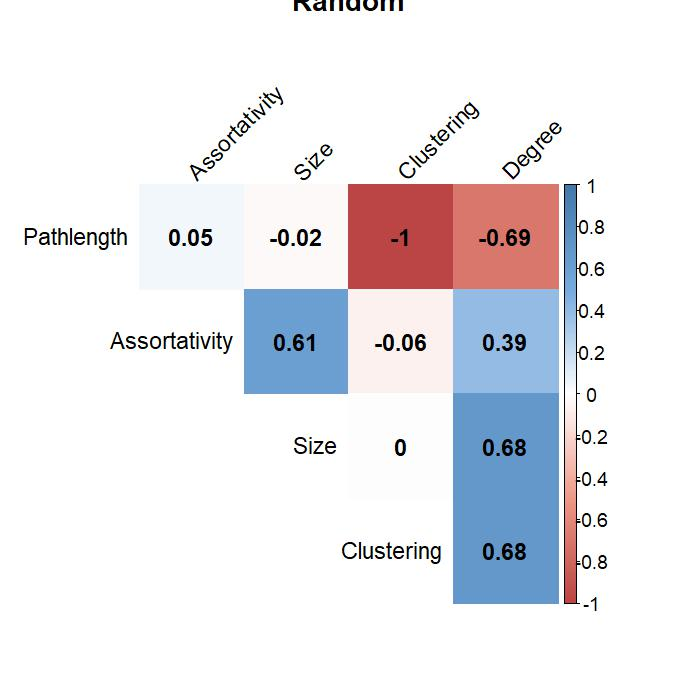
\includegraphics{./Figures/unnamed-chunk-75-1} 

}

\caption{Distribution of the data in scale-free networks.}\label{fig:unnamed-chunk-75}
\end{figure}

\textbf{Small-world networks}

\begin{longtable}[]{@{}
  >{\raggedright\arraybackslash}p{(\columnwidth - 20\tabcolsep) * \real{0.0194}}
  >{\raggedright\arraybackslash}p{(\columnwidth - 20\tabcolsep) * \real{0.0516}}
  >{\raggedright\arraybackslash}p{(\columnwidth - 20\tabcolsep) * \real{0.1097}}
  >{\raggedright\arraybackslash}p{(\columnwidth - 20\tabcolsep) * \real{0.0839}}
  >{\raggedright\arraybackslash}p{(\columnwidth - 20\tabcolsep) * \real{0.0903}}
  >{\raggedright\arraybackslash}p{(\columnwidth - 20\tabcolsep) * \real{0.1097}}
  >{\raggedright\arraybackslash}p{(\columnwidth - 20\tabcolsep) * \real{0.1290}}
  >{\raggedright\arraybackslash}p{(\columnwidth - 20\tabcolsep) * \real{0.0774}}
  >{\raggedright\arraybackslash}p{(\columnwidth - 20\tabcolsep) * \real{0.1161}}
  >{\raggedright\arraybackslash}p{(\columnwidth - 20\tabcolsep) * \real{0.0968}}
  >{\raggedright\arraybackslash}p{(\columnwidth - 20\tabcolsep) * \real{0.1161}}@{}}
\toprule()
\begin{minipage}[b]{\linewidth}\raggedright
\end{minipage} & \begin{minipage}[b]{\linewidth}\raggedright
size
\end{minipage} & \begin{minipage}[b]{\linewidth}\raggedright
clustering
\end{minipage} & \begin{minipage}[b]{\linewidth}\raggedright
node\_degree
\end{minipage} & \begin{minipage}[b]{\linewidth}\raggedright
pathlength
\end{minipage} & \begin{minipage}[b]{\linewidth}\raggedright
assortativity
\end{minipage} & \begin{minipage}[b]{\linewidth}\raggedright
init\_lang\_exp
\end{minipage} & \begin{minipage}[b]{\linewidth}\raggedright
rewire
\end{minipage} & \begin{minipage}[b]{\linewidth}\raggedright
inter\_var
\end{minipage} & \begin{minipage}[b]{\linewidth}\raggedright
mean\_intra\_var
\end{minipage} & \begin{minipage}[b]{\linewidth}\raggedright
std\_intra\_var
\end{minipage} \\
\midrule()
\endhead
& 50 :300 & Min. :0.001556 & Min. : 4 & Min. :1.020 & Min. :-0.29315 &
With (strong):300 & Min. :0.1 & Min. :2.030e-07 & Min. :0.8495 & Min.
:0.0001095 \\
& 150:300 & 1st Qu.:0.100506 & 1st Qu.: 7 & 1st Qu.:1.829 & 1st
Qu.:-0.06832 & With (weak) :300 & 1st Qu.:0.3 & 1st Qu.:4.184e-05 & 1st
Qu.:1.2909 & 1st Qu.:0.0028076 \\
& 300:300 & Median :0.232127 & Median :12 & Median :2.364 & Median
:-0.03556 & Without :300 & Median :0.5 & Median :3.634e-04 & Median
:1.9660 & Median :0.0087059 \\
& NA & Mean :0.296572 & Mean :19 & Mean :2.635 & Mean :-0.04476 & NA &
Mean :0.5 & Mean :2.291e-03 & Mean :1.8188 & Mean :0.0184484 \\
& NA & 3rd Qu.:0.399529 & 3rd Qu.:24 & 3rd Qu.:3.071 & 3rd Qu.:-0.01115
& NA & 3rd Qu.:0.7 & 3rd Qu.:2.709e-03 & 3rd Qu.:2.2501 & 3rd
Qu.:0.0275223 \\
& NA & Max. :0.980213 & Max. :48 & Max. :7.277 & Max. : 0.11942 & NA &
Max. :0.9 & Max. :3.078e-02 & Max. :2.2993 & Max. :0.1244774 \\
\bottomrule()
\end{longtable}

In small-world networks, the only structural parameters we manipulated
were the \emph{rewiring} probability (0.1, 0.3, 0.5, 0.7, 0.9), the
\emph{node degree} (4, 8, 16, 48 neighbors), and the \emph{size} (50,
150, and 300).

For simplicity reasons, we do not plot here the node degree as a facet.

\begin{figure}[!H]

{\centering 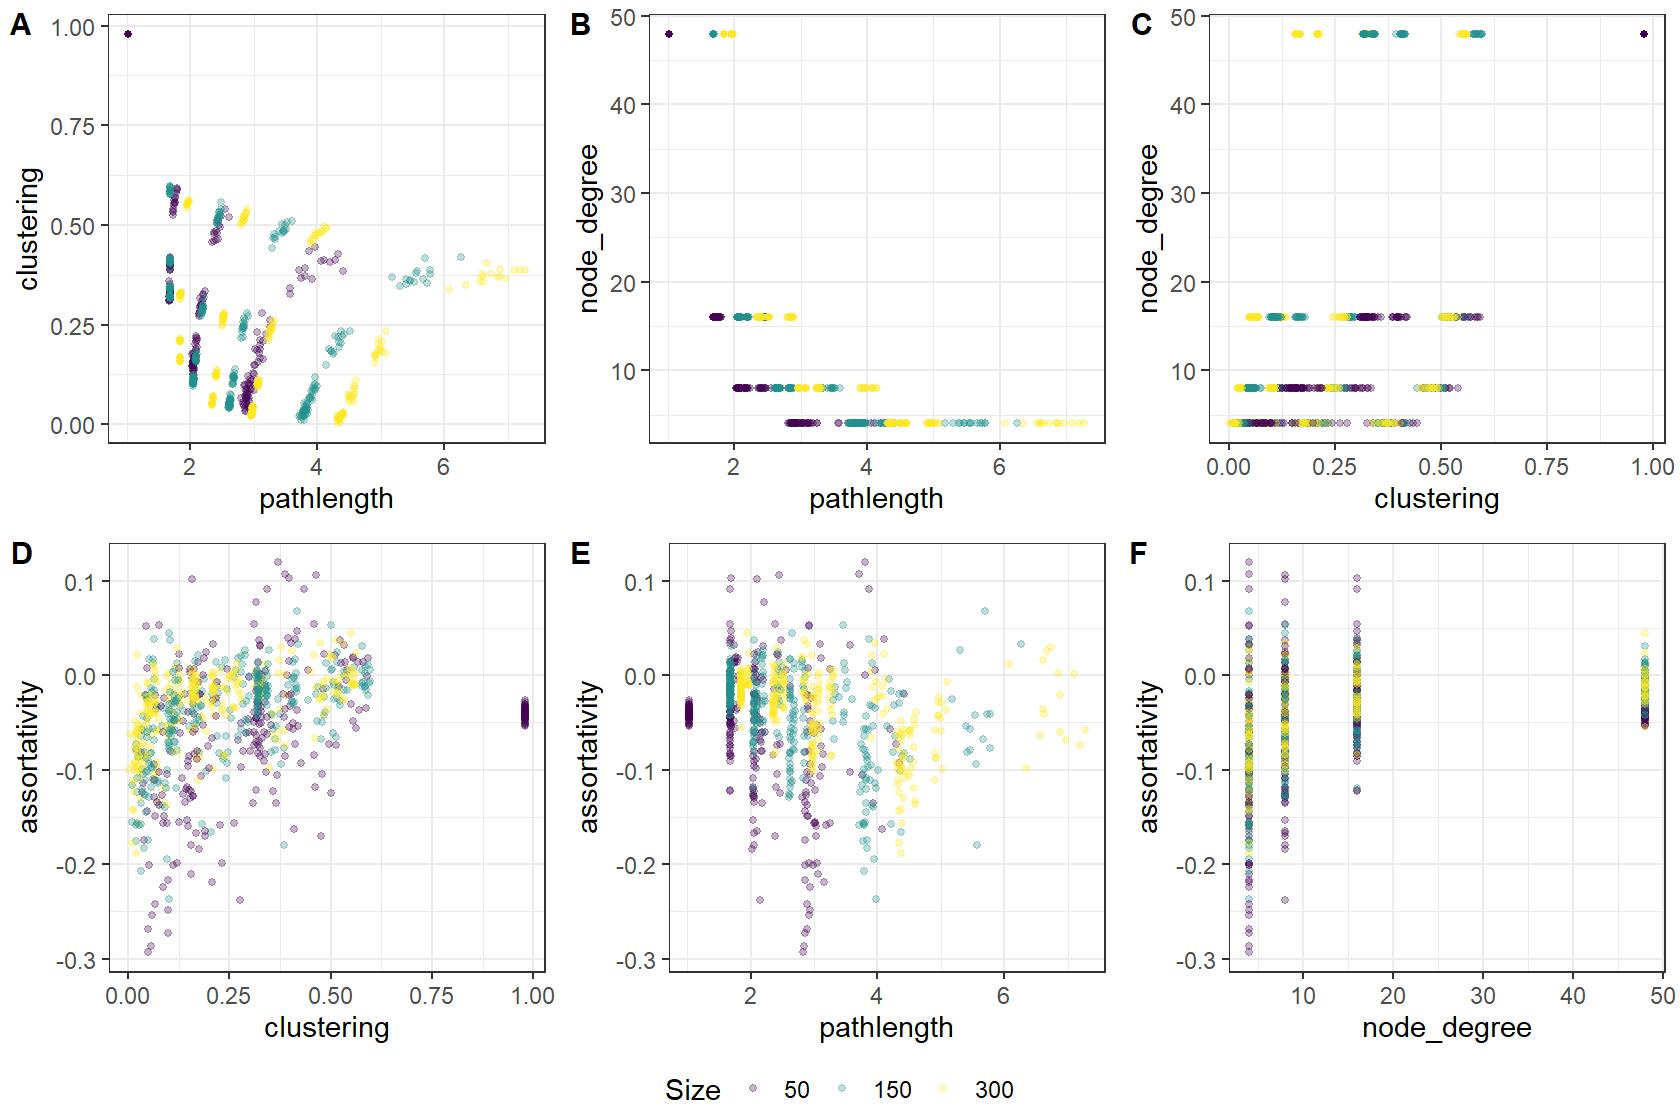
\includegraphics{./Figures/unnamed-chunk-77-1} 

}

\caption{Distribution of the data in small-world networks.}\label{fig:unnamed-chunk-77}
\end{figure}

\hypertarget{correlations}{%
\subsubsection{Correlations}\label{correlations}}

The data is \textbf{\emph{not}} normally distributed. So we should use
Spearman's correlations instead of Pearson's correlations. Since it does
not cost much to compute both, you can find below both of them :)

Please note that I didn't manage to put them in grid.arrange all
together.

\textbf{Pearson's correlations}:

\begin{figure}[!H]

{\centering 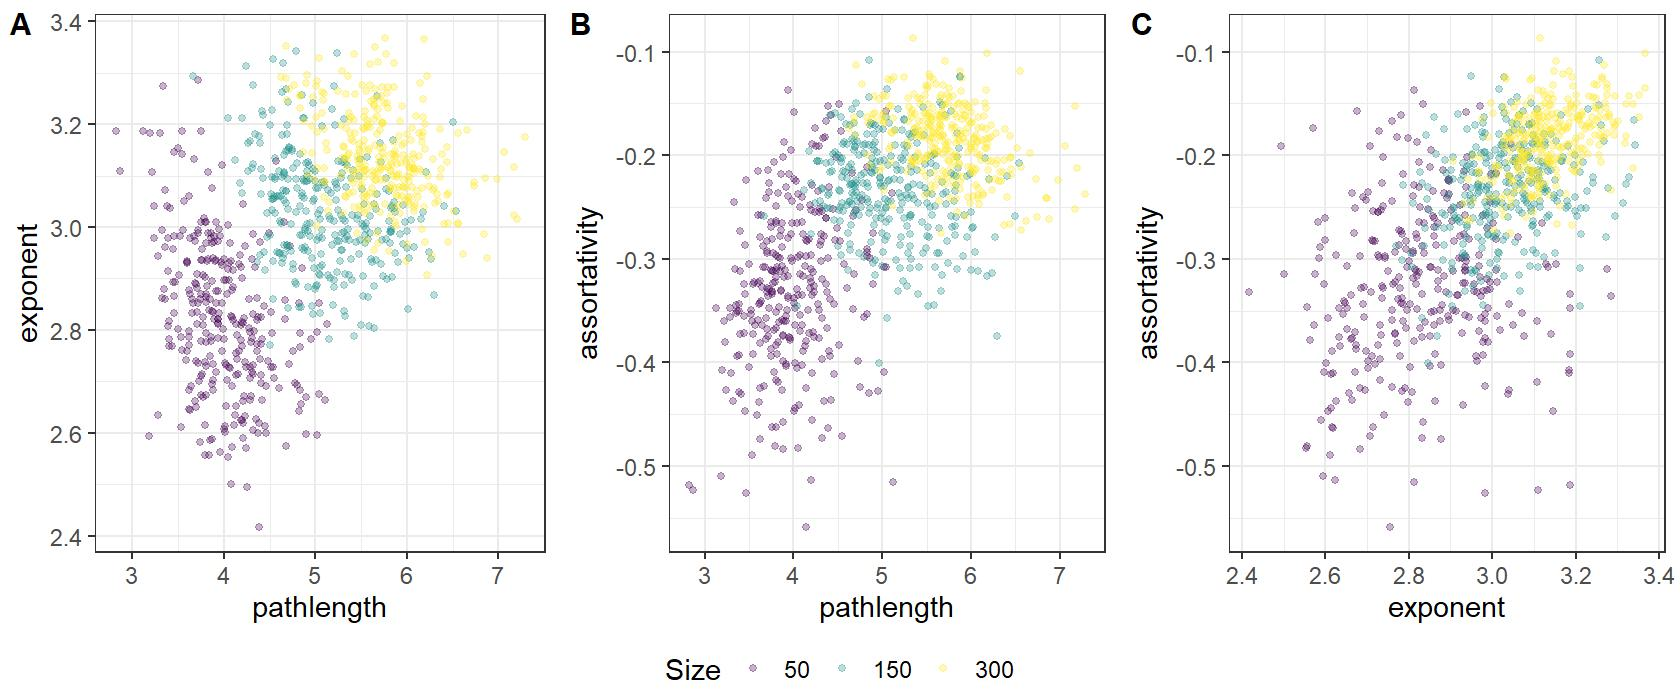
\includegraphics{./Figures/unnamed-chunk-78-1} 

}

\caption{Pearsons correlations.}\label{fig:unnamed-chunk-78-1}
\end{figure}
\begin{figure}[!H]

{\centering 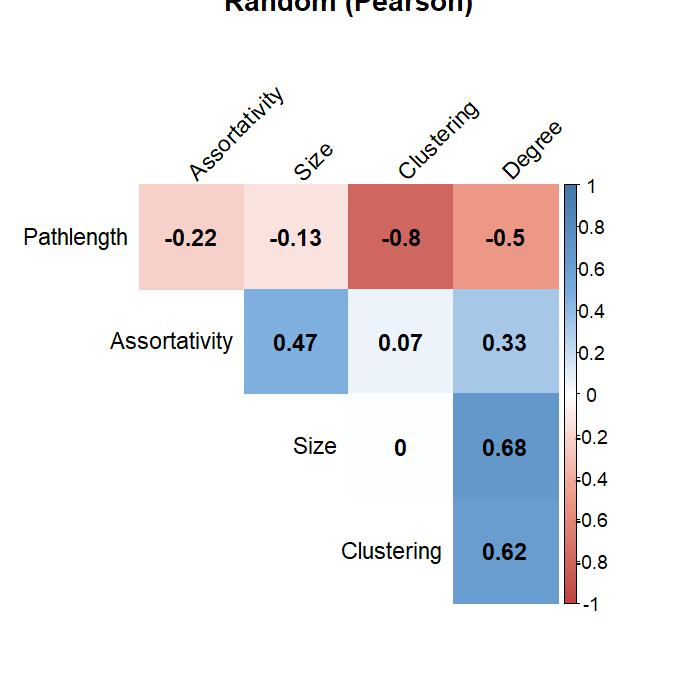
\includegraphics{./Figures/unnamed-chunk-78-2} 

}

\caption{Pearsons correlations.}\label{fig:unnamed-chunk-78-2}
\end{figure}
\begin{figure}[!H]

{\centering 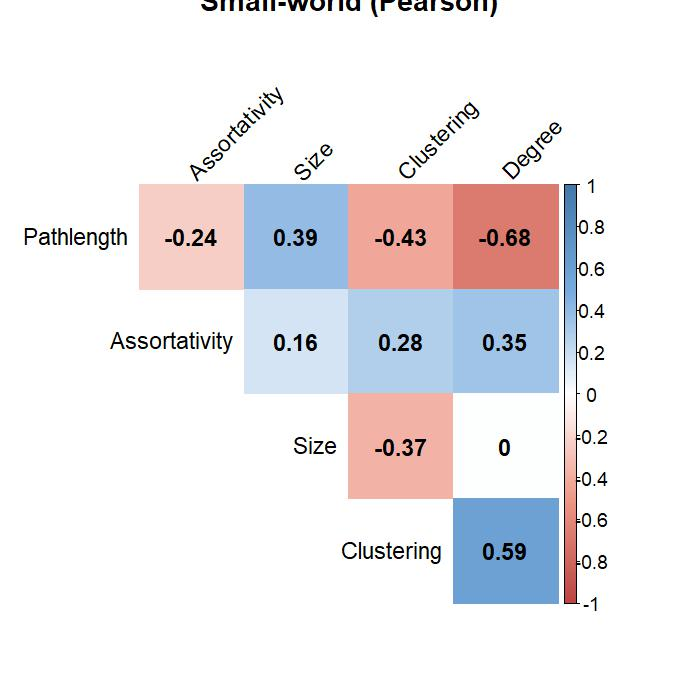
\includegraphics{./Figures/unnamed-chunk-78-3} 

}

\caption{Pearsons correlations.}\label{fig:unnamed-chunk-78-3}
\end{figure}

\textbf{Spearman's correlations}:

\begin{figure}[!H]

{\centering 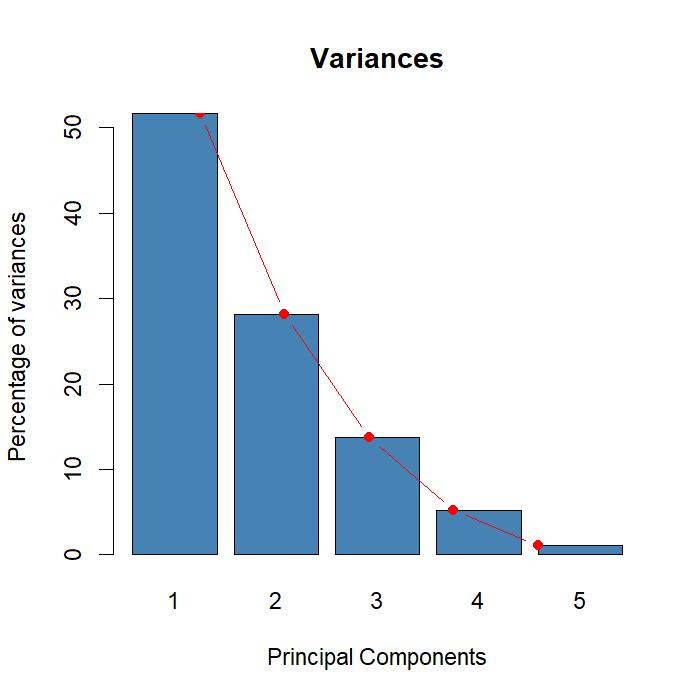
\includegraphics{./Figures/unnamed-chunk-79-1} 

}

\caption{Spearmans correlations.}\label{fig:unnamed-chunk-79-1}
\end{figure}
\begin{figure}[!H]

{\centering 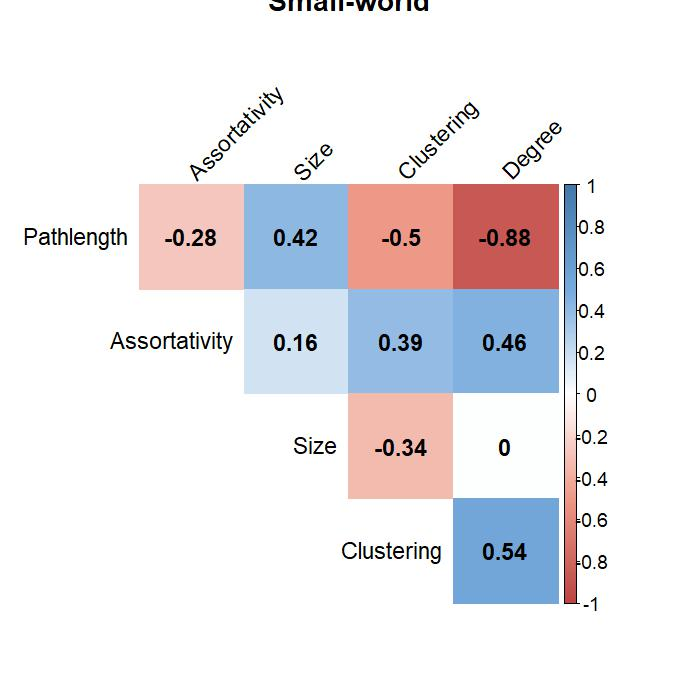
\includegraphics{./Figures/unnamed-chunk-79-2} 

}

\caption{Spearmans correlations.}\label{fig:unnamed-chunk-79-2}
\end{figure}
\begin{figure}[!H]

{\centering 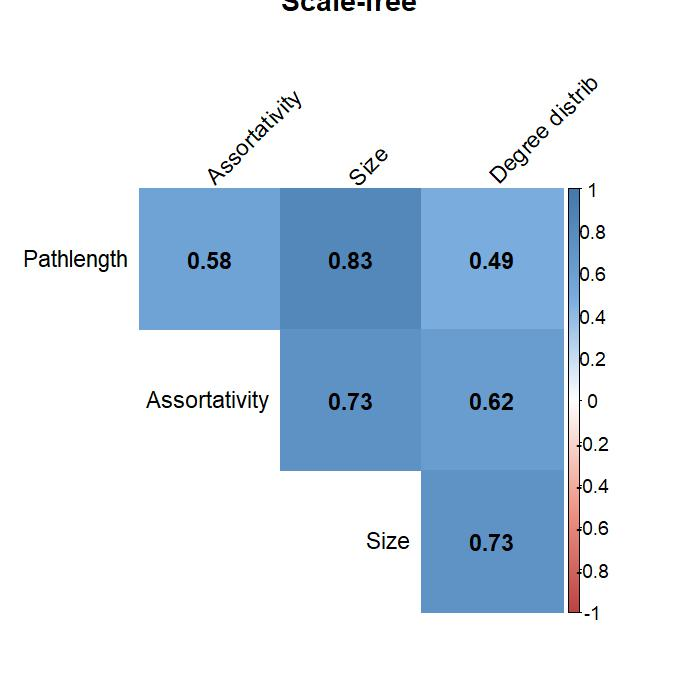
\includegraphics{./Figures/unnamed-chunk-79-3} 

}

\caption{Spearmans correlations.}\label{fig:unnamed-chunk-79-3}
\end{figure}

We found high correlations between some variables. In order to
understand the direction of correlation, we graphically print the
relationships between the metrics in all types of networks. Size will
always be printed in a color layer.

\textbf{Random networks}:

\begin{figure}[!H]

{\centering 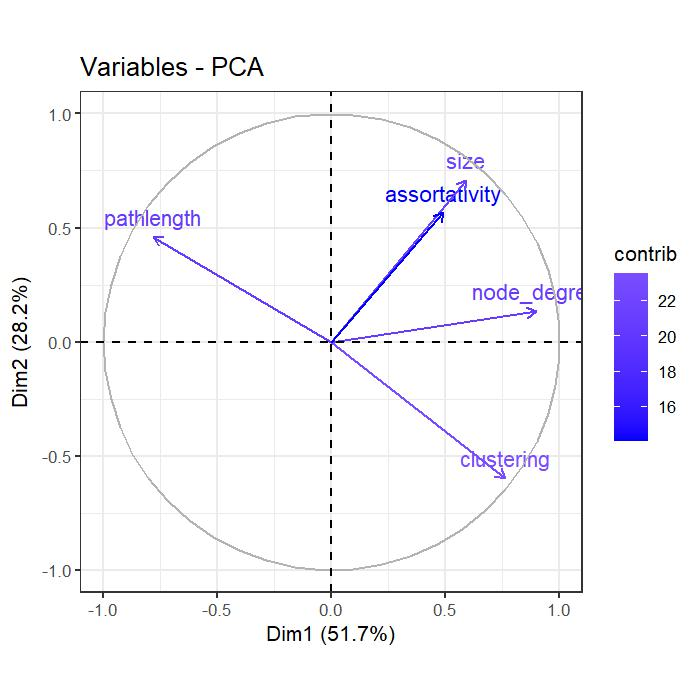
\includegraphics{./Figures/unnamed-chunk-80-1} 

}

\caption{Graphical visualization of the relationship between the metrics using a range of random networks.}\label{fig:unnamed-chunk-80}
\end{figure}

Please note that we ran several simulation with random network using
different connection probability and size of the network, which
correspond to the different bumps in the visualization.

\textbf{Small-world networks}:

\begin{figure}[!H]

{\centering 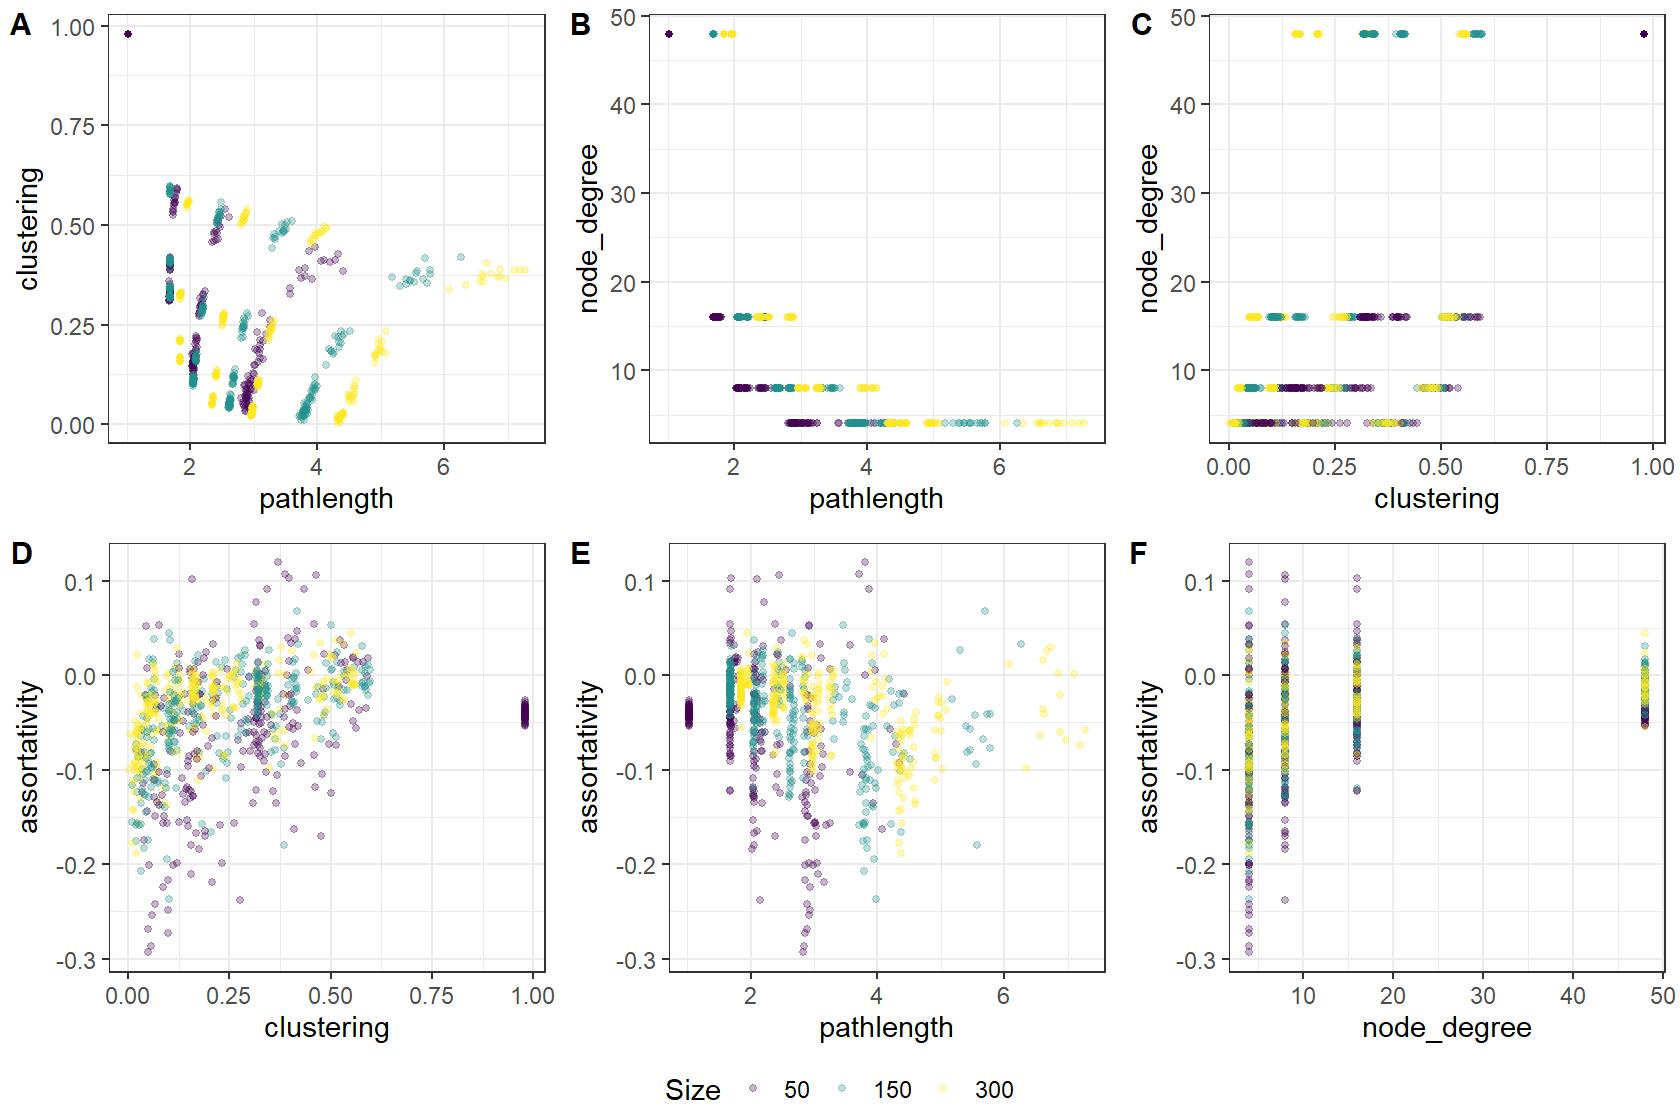
\includegraphics{./Figures/unnamed-chunk-81-1} 

}

\caption{Graphical visualization of the relationship between the metrics using a range of small-world networks.}\label{fig:unnamed-chunk-81}
\end{figure}

Please note that we ran several simulation with small-world network
using different rewiring probability, node degree, and size of the
network, which correspond to the different bumps in the visualization.

\textbf{Scale-free networks}:

\begin{figure}[!H]

{\centering 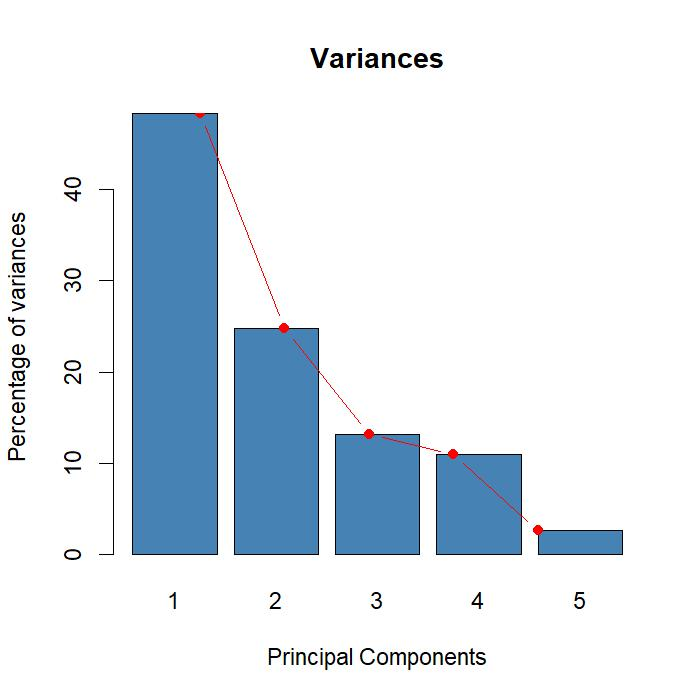
\includegraphics{./Figures/unnamed-chunk-82-1} 

}

\caption{Graphical visualization of the relationship between the metrics using a range of scale-free networks.}\label{fig:unnamed-chunk-82}
\end{figure}

\hypertarget{principal-component-analysis}{%
\subsubsection{Principal Component
Analysis}\label{principal-component-analysis}}

We also look at the PCA between these metrics in all types of networks.

\textbf{Random networks}:

\begin{figure}[!H]

{\centering 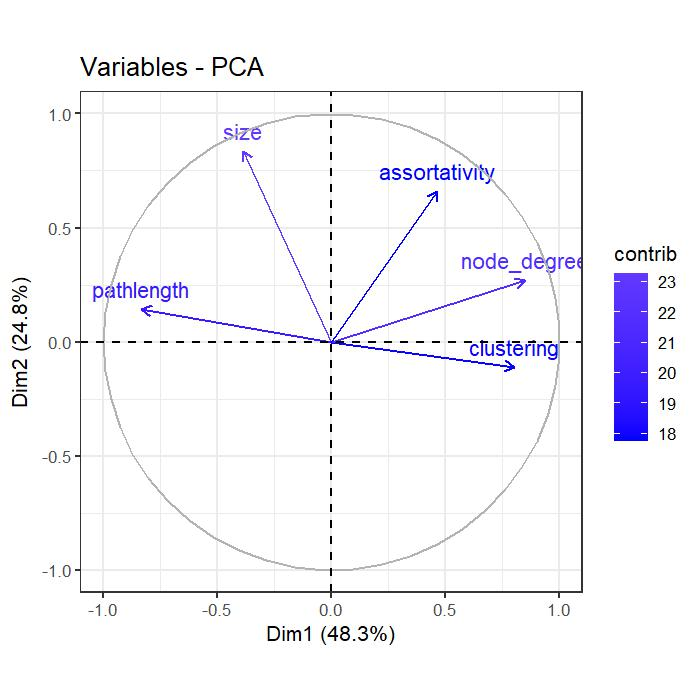
\includegraphics{./Figures/unnamed-chunk-83-1} 

}

\caption{Histogram of the eigenvalues of the PCA between the metrics using a range of random networks.}\label{fig:unnamed-chunk-83}
\end{figure}

\begin{figure}[!H]

{\centering 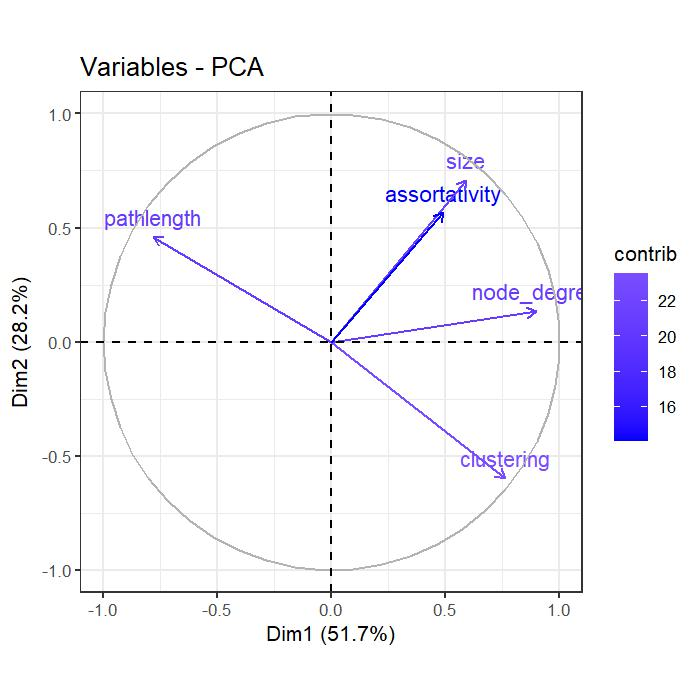
\includegraphics{./Figures/unnamed-chunk-84-1} 

}

\caption{Contribution of the different metrics in the PCA using a range of random networks.}\label{fig:unnamed-chunk-84}
\end{figure}

\textbf{Small-world networks}:

\begin{figure}[!H]

{\centering 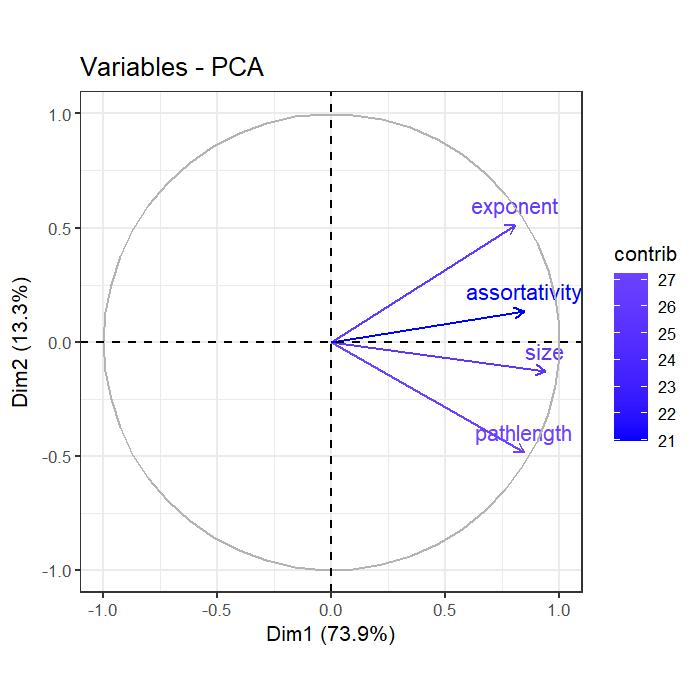
\includegraphics{./Figures/unnamed-chunk-86-1} 

}

\caption{Histogram of the eigenvalues of the PCA between the metrics using a range of small-world networks.}\label{fig:unnamed-chunk-86}
\end{figure}

\begin{figure}[!H]

{\centering 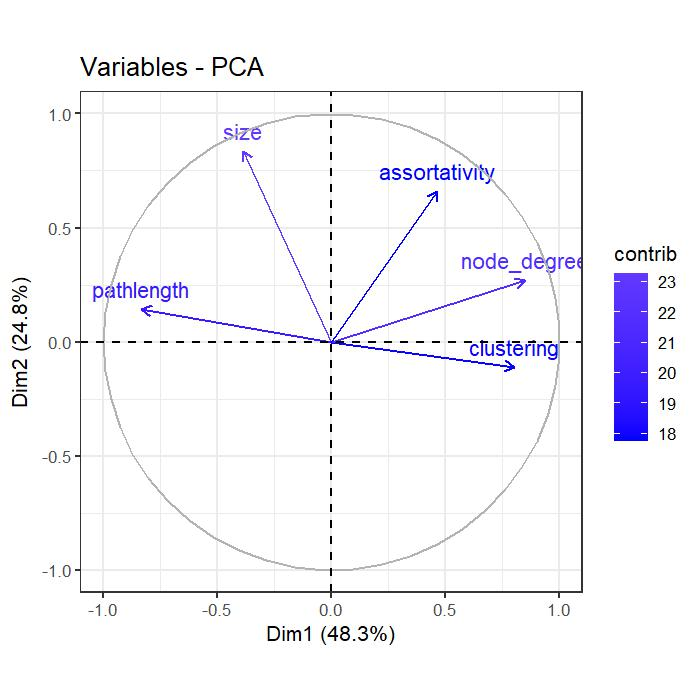
\includegraphics{./Figures/unnamed-chunk-87-1} 

}

\caption{Contribution of the different metrics in the PCA using a range of small-world networks.}\label{fig:unnamed-chunk-87}
\end{figure}

\textbf{Scale-free networks}:

\begin{figure}[!H]

{\centering 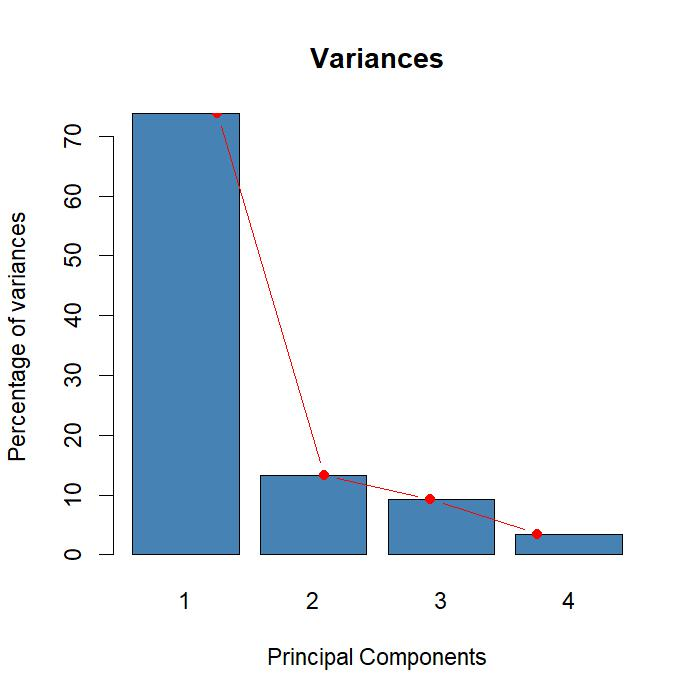
\includegraphics{./Figures/unnamed-chunk-89-1} 

}

\caption{Histogram of the eigenvalues of the PCA between the metrics using a range of scale-free networks.}\label{fig:unnamed-chunk-89}
\end{figure}

\begin{figure}[!H]

{\centering 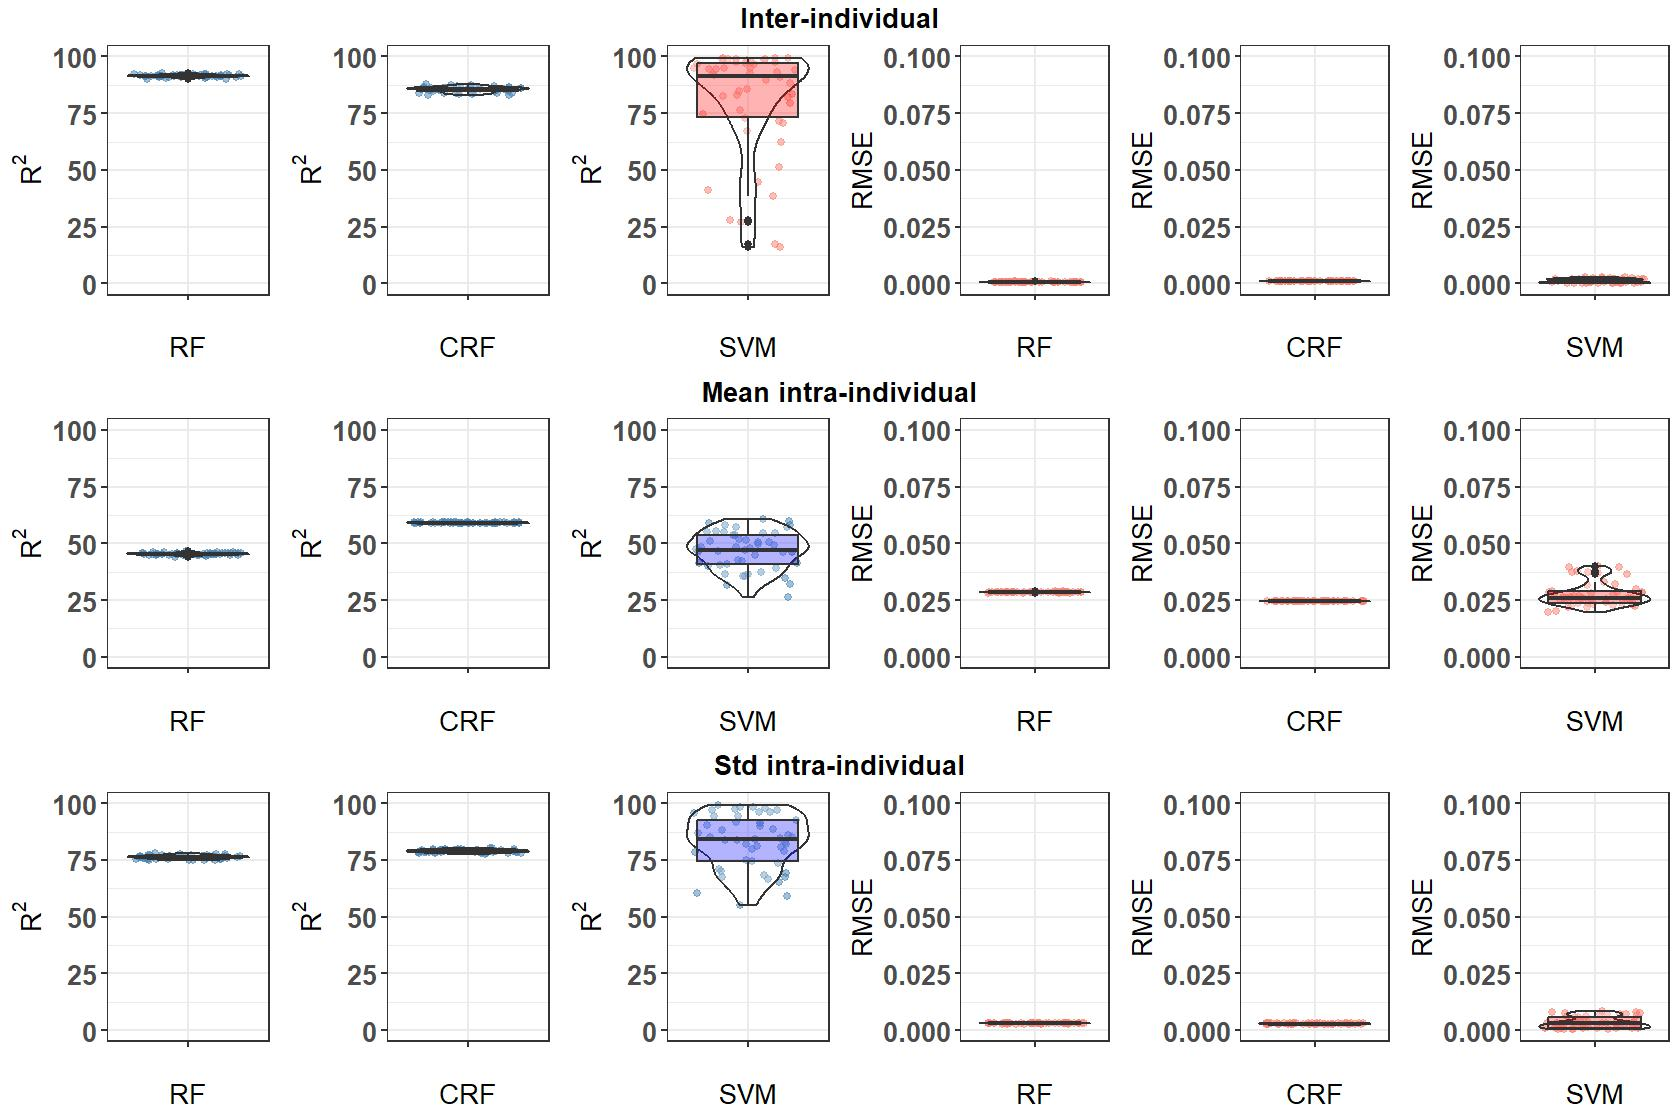
\includegraphics{./Figures/unnamed-chunk-90-1} 

}

\caption{Contribution of the different metrics in the PCA using a range of scale-free networks.}\label{fig:unnamed-chunk-90}
\end{figure}

\hypertarget{machine-learning-rf-cf-svm}{%
\subsubsection{Machine learning (RF, CF \&
SVM)}\label{machine-learning-rf-cf-svm}}

We predict variation (inter, mean intra, and std intra) from a
collection of potential predictors using three machine learning
techniques:

\begin{itemize}
\item
  \textbf{random forests (RF)}: as implemented by
  \texttt{randomForest()} in package \texttt{randomForest}. This
  function implements Breiman's random forest algorithm (based on
  Breiman and Cutler's original Fortran code); see
  \href{https://www.rdocumentation.org/packages/randomForest/versions/4.7-1.1/topics/randomForest}{here}
  for more information. RF have been shown to be particularly relevant
  when predictors are inter-correlated (see Levshina, 2021, in the
  Chapter 25 ``Conditional Inference Trees and Random Forests''). We
  extract the predictor importance using two indexes: the
  \emph{accuracy-based} index and the \emph{gini-based} index. The
  accuracy-based index measures the reduction in model accuracy if a
  particular predictor is removed or permuted. On the other hand, the
  Gini Index is a measure of impurity or purity in a decision tree. In
  the context of random forests, namely, it measures how often a
  randomly chosen element from the dataset would be incorrectly labeled
  if it was randomly labeled according to the distribution of labels in
  the node.
\item
  \textbf{conditional random forests} (CF): as implemented by
  \texttt{cforest()} in package \texttt{partykit}. The number of trees
  is 200, and the number of permutations is 10. We measured the
  predictor importance using the \emph{unconditional} index. The
  unconditional index for a given predictor measures how well that
  predictor alone, in isolation, can help to improve the predictive
  accuracy of the model.
\item
  \textbf{support vector machines} (SVM): as implemented by
  \texttt{fit(...,model="svm")} in the \texttt{rminer} package; see
  \href{https://rdrr.io/cran/rminer/man/fit.html}{here}). We used a
  regression task (since the output is continuous). This function uses
  \texttt{ksvm} from \texttt{kernlab} package; more information on this
  function can be found
  \href{https://www.rdocumentation.org/packages/kernlab/versions/0.9-32/topics/ksvm}{here}.
  We measured the predictor importance based on \emph{sensitivity}
  analysis. The sensitivity method for predictor importance in SVM
  involves perturbing individual predictors to observe the resulting
  changes in the model's output, quantifying the impact, and ranking
  predictors based on their sensitivity scores to identify the most
  influential features in the SVM decision-making process.
\end{itemize}

For each method, we extract some success measures, here the \emph{R²}
and RMSE using \texttt{postResample} function of \texttt{rminer}
package. Note that we z-scored all the predictors.

\hypertarget{random-networks}{%
\paragraph{Random networks}\label{random-networks}}

\textbf{Success} in language \textbf{emergence} context:

\emph{Inter-individual variation}:

\begin{itemize}
\tightlist
\item
  random forests: R\textsuperscript{2} = 91.5\% ±0.6\%, RMSE = 0.001
  ±0.000
\item
  conditional random forests: R\textsuperscript{2} = 85.5\% ±1.2\%, RMSE
  = 0.001 ±0.000.
\item
  support vector machines: R\textsuperscript{2} = 80.4\% ±23.4\%, RMSE =
  0.001 ±0.001.
\end{itemize}

\emph{Mean Intra-individual variation}:

\begin{itemize}
\tightlist
\item
  random forests: R\textsuperscript{2} = 45.3\% ±0.5\%, RMSE = 0.029
  ±0.000
\item
  conditional random forests: R\textsuperscript{2} = 59.1\% ±0.2\%, RMSE
  = 0.025 ±0.000.
\item
  support vector machines: R\textsuperscript{2} = 46.8\% ±8.3\%, RMSE =
  0.028 ±0.005.
\end{itemize}

\emph{Std Intra-individual variation}:

\begin{itemize}
\tightlist
\item
  random forests: R\textsuperscript{2} = 76.3\% ±0.8\%, RMSE = 0.003
  ±0.000
\item
  conditional random forests: R\textsuperscript{2} = 79.0\% ±0.6\%, RMSE
  = 0.003 ±0.000.
\item
  support vector machines: R\textsuperscript{2} = 83.1\% ±11.7\%, RMSE =
  0.003 ±0.003.
\end{itemize}

Let's plot this data:

\begin{figure}[!H]

{\centering 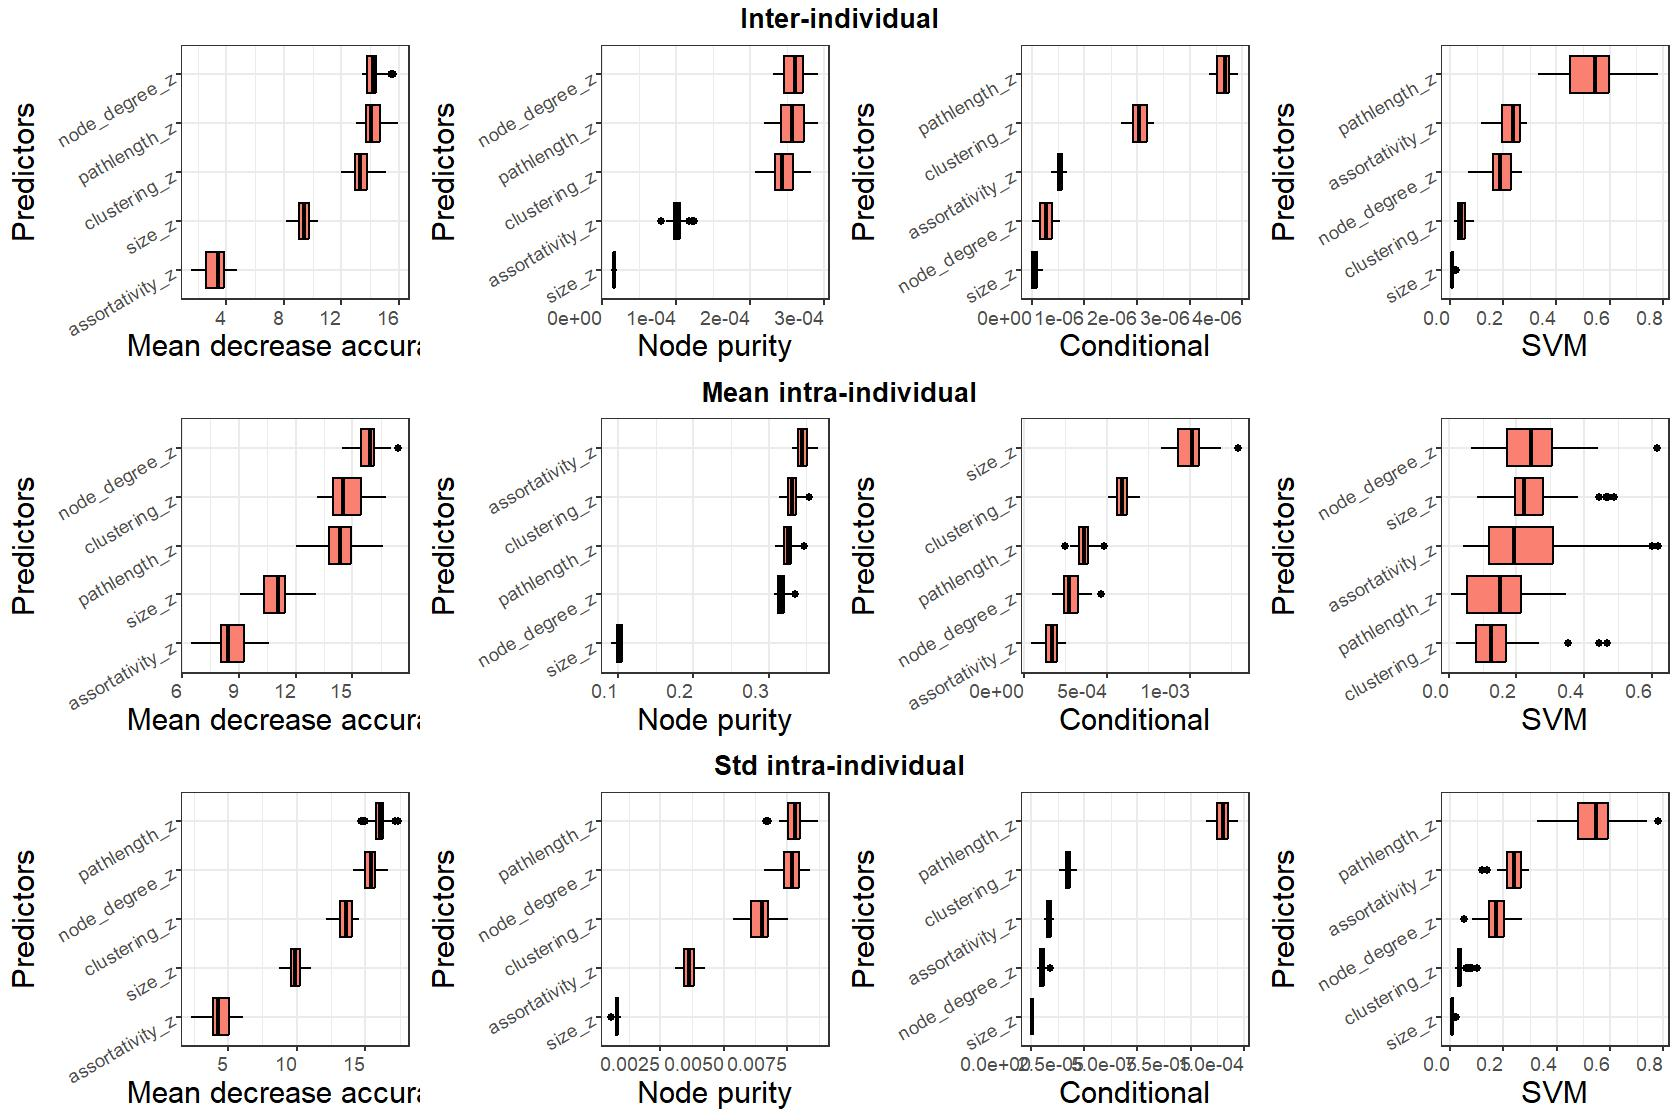
\includegraphics{./Figures/unnamed-chunk-94-1} 

}

\caption{Success (using R² and RMSE indexes) in random networks in language emergence scenarios for each type of method.}\label{fig:unnamed-chunk-94}
\end{figure}

\textbf{Predictor importance} in language emergence context:

Important: note that the metrics are printed by decreasing importance,
so their order may vary between the different methods!

\begin{figure}[!H]

{\centering 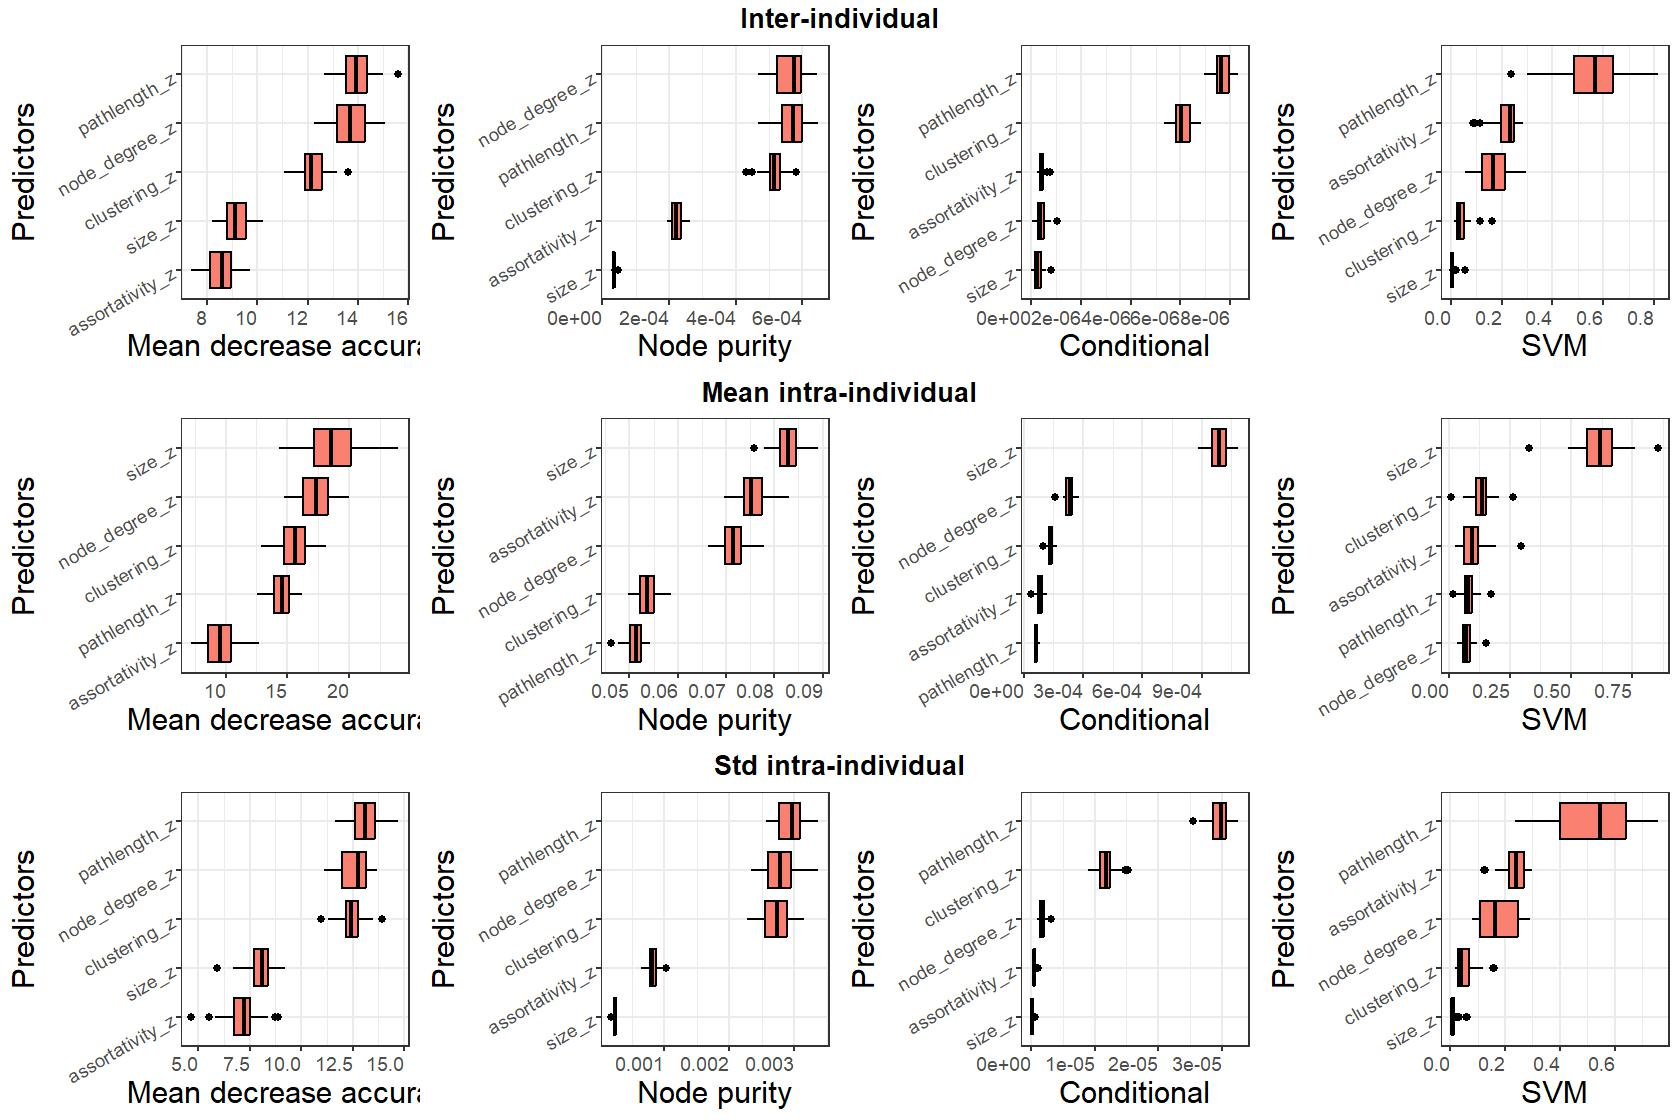
\includegraphics{./Figures/unnamed-chunk-95-1} 

}

\caption{Predictor importance in random networks in language emergence scenarios for each type of method.}\label{fig:unnamed-chunk-95}
\end{figure}

\textbf{Success} in language \textbf{change} context:

\emph{Inter-individual variation}:

\begin{itemize}
\tightlist
\item
  random forests: R\textsuperscript{2} = 95.9\% ±0.4\%, RMSE = 0.000
  ±0.000
\item
  conditional random forests: R\textsuperscript{2} = 82.9\% ±1.2\%, RMSE
  = 0.001 ±0.000.
\item
  support vector machines: R\textsuperscript{2} = 88.5\% ±15.0\%, RMSE =
  0.001 ±0.001.
\end{itemize}

\emph{Mean Intra-individual variation}:

\begin{itemize}
\tightlist
\item
  random forests: R\textsuperscript{2} = 2.5\% ±0.7\%, RMSE = 0.086
  ±0.000
\item
  conditional random forests: R\textsuperscript{2} = 26.3\% ±0.2\%, RMSE
  = 0.075 ±0.000.
\item
  support vector machines: R\textsuperscript{2} = 4.3\% ±4.8\%, RMSE =
  0.093 ±0.009.
\end{itemize}

\emph{Std Intra-individual variation}:

\begin{itemize}
\tightlist
\item
  random forests: R\textsuperscript{2} = 90.3\% ±0.4\%, RMSE = 0.003
  ±0.000
\item
  conditional random forests: R\textsuperscript{2} = 85.2\% ±0.8\%, RMSE
  = 0.004 ±0.000.
\item
  support vector machines: R\textsuperscript{2} = 86.8\% ±12.9\%, RMSE =
  0.004 ±0.003.
\end{itemize}

\begin{figure}[!H]

{\centering 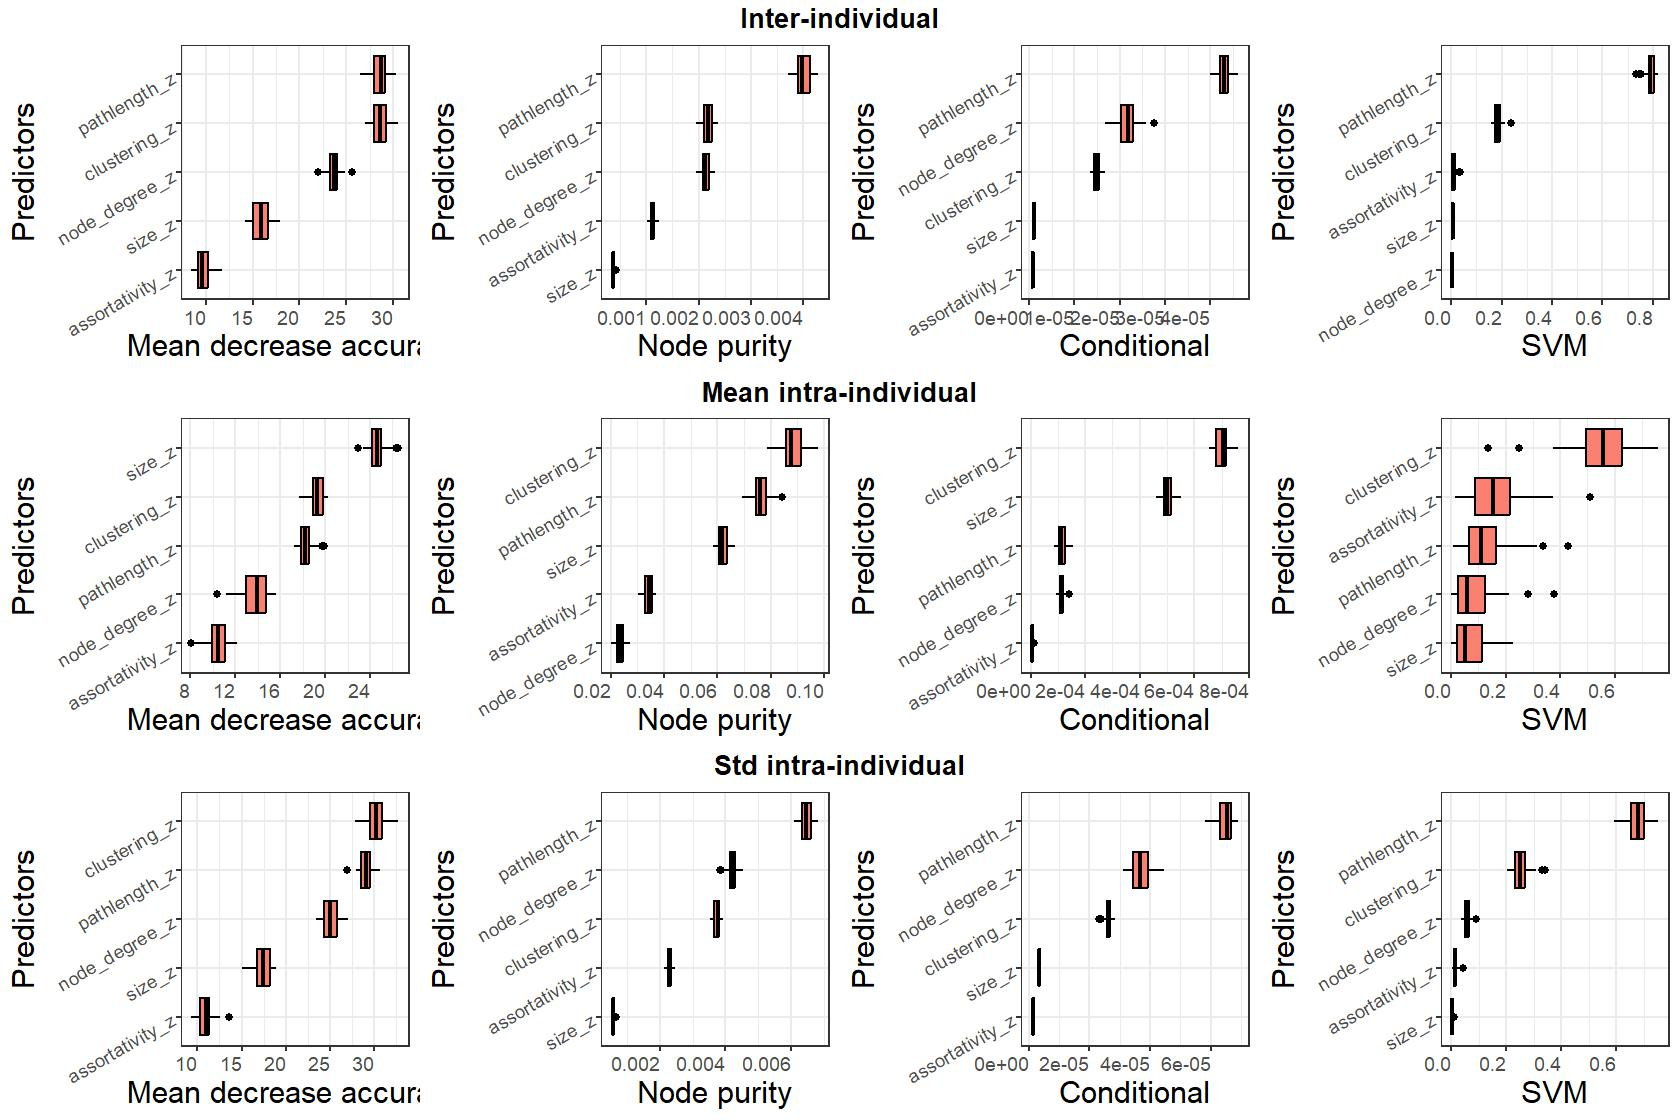
\includegraphics{./Figures/unnamed-chunk-97-1} 

}

\caption{Success (using R² and RMSE indexes) in random networks in language change scenario for each type of method.}\label{fig:unnamed-chunk-97}
\end{figure}

\textbf{Predictor importance} in language change context:

Important: note that the metrics are printed by decreasing importance,
so their order may vary between the different methods!

\begin{figure}[!H]

{\centering 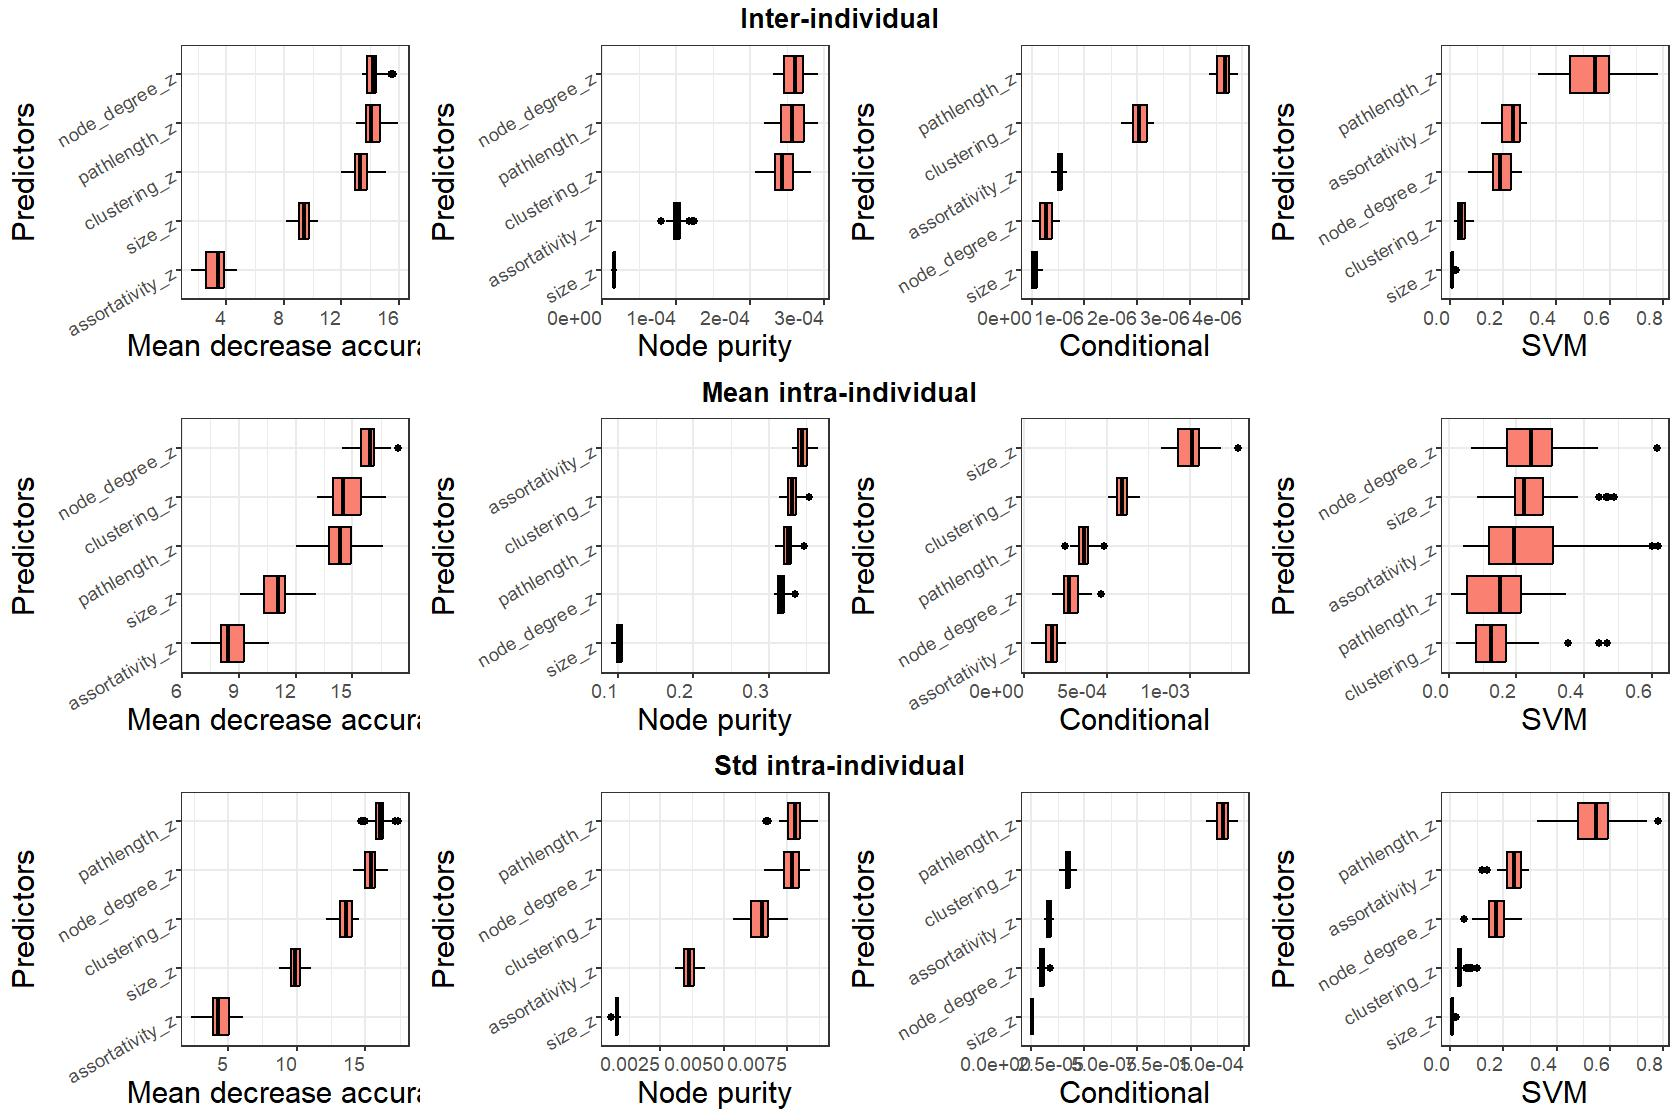
\includegraphics{./Figures/unnamed-chunk-98-1} 

}

\caption{Predictor importance in random networks in language change scenario for each type of method.}\label{fig:unnamed-chunk-98}
\end{figure}

\hypertarget{small-world-networks}{%
\paragraph{Small-world networks}\label{small-world-networks}}

\textbf{Success} in language \textbf{emergence} context:

\emph{Inter-individual variation}:

\begin{itemize}
\tightlist
\item
  random forests: R\textsuperscript{2} = 90.2\% ±0.5\%, RMSE = 0.002
  ±0.000
\item
  conditional random forests: R\textsuperscript{2} = 95.3\% ±0.2\%, RMSE
  = 0.001 ±0.000.
\item
  support vector machines: R\textsuperscript{2} = 92.8\% ±2.2\%, RMSE =
  0.001 ±0.000.
\end{itemize}

\emph{Mean Intra-individual variation}:

\begin{itemize}
\tightlist
\item
  random forests: R\textsuperscript{2} = 58.9\% ±0.4\%, RMSE = 0.024
  ±0.000
\item
  conditional random forests: R\textsuperscript{2} = 67.3\% ±0.2\%, RMSE
  = 0.021 ±0.000.
\item
  support vector machines: R\textsuperscript{2} = 7.0\% ±7.1\%, RMSE =
  0.070 ±0.008.
\end{itemize}

\emph{Std Intra-individual variation}:

\begin{itemize}
\tightlist
\item
  random forests: R\textsuperscript{2} = 81.6\% ±0.4\%, RMSE = 0.004
  ±0.000
\item
  conditional random forests: R\textsuperscript{2} = 89.0\% ±0.2\%, RMSE
  = 0.003 ±0.000.
\item
  support vector machines: R\textsuperscript{2} = 84.6\% ±5.0\%, RMSE =
  0.009 ±0.002.
\end{itemize}

\begin{figure}[!H]

{\centering 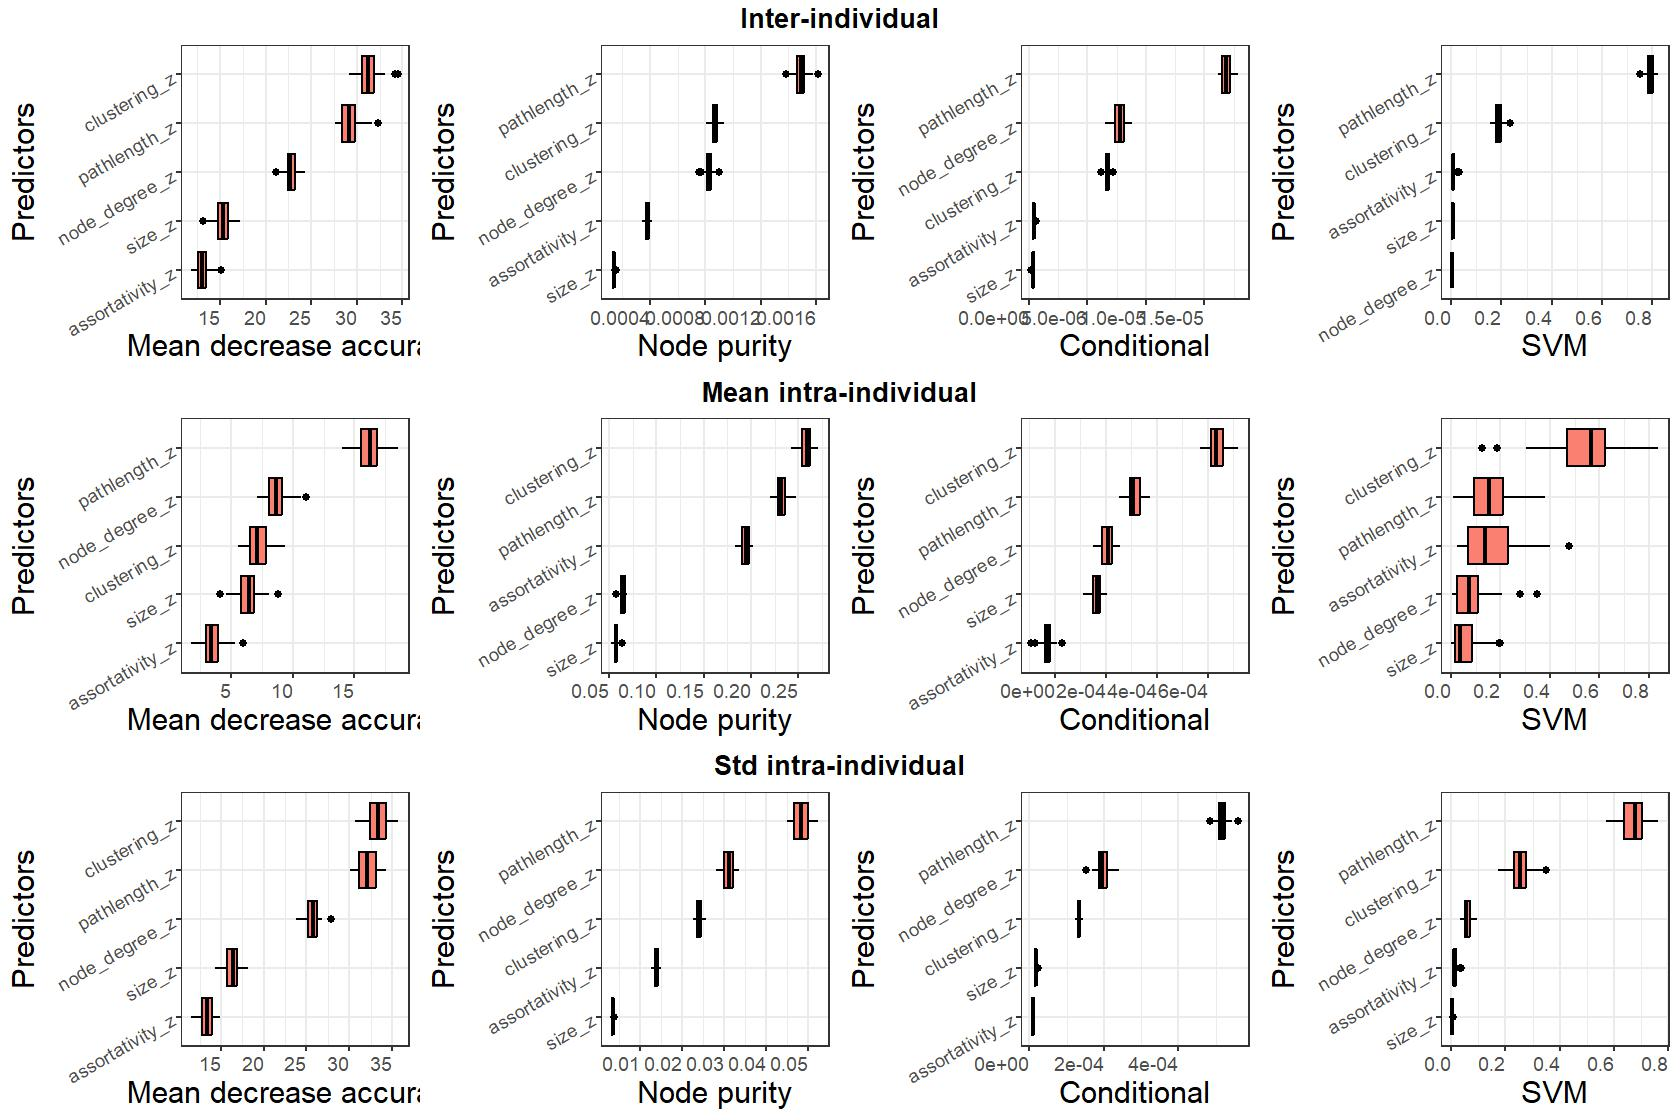
\includegraphics{./Figures/unnamed-chunk-100-1} 

}

\caption{Success (using R² and RMSE indexes) in small-world networks in language emergence scenario for each type of method.}\label{fig:unnamed-chunk-100}
\end{figure}

\textbf{Predictor importance} in language emergence context:

Important: note that the metrics are printed by decreasing importance,
so their order may vary between the different methods!

\begin{figure}[!H]

{\centering 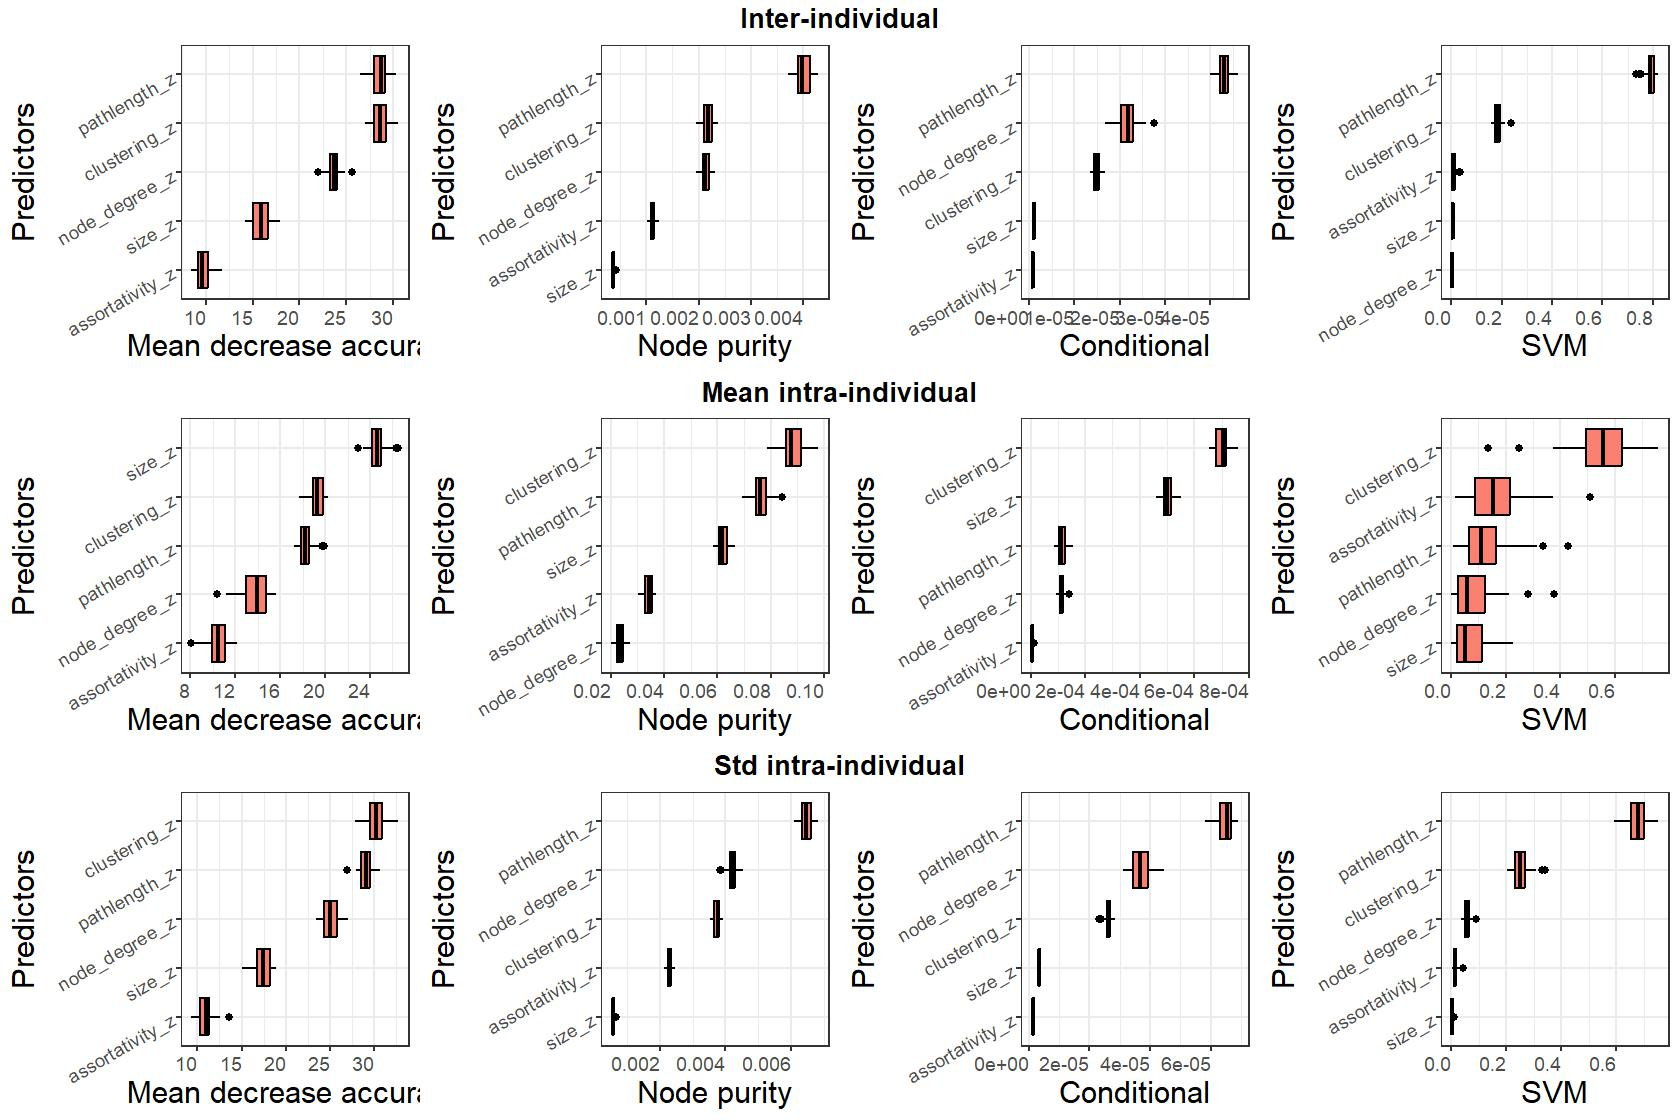
\includegraphics{./Figures/unnamed-chunk-101-1} 

}

\caption{Predictor importance in small-world networks in language emergence scenario for each type of method.}\label{fig:unnamed-chunk-101}
\end{figure}

\textbf{Success} in language \textbf{change} context:

\emph{Inter-individual variation}:

\begin{itemize}
\tightlist
\item
  random forests: R\textsuperscript{2} = 88.0\% ±0.5\%, RMSE = 0.001
  ±0.000
\item
  conditional random forests: R\textsuperscript{2} = 93.2\% ±0.2\%, RMSE
  = 0.001 ±0.000.
\item
  support vector machines: R\textsuperscript{2} = 92.9\% ±2.8\%, RMSE =
  0.001 ±0.000.
\end{itemize}

\emph{Mean Intra-individual variation}:

\begin{itemize}
\tightlist
\item
  random forests: R\textsuperscript{2} = 4.7\% ±0.7\%, RMSE = 0.072
  ±0.000
\item
  conditional random forests: R\textsuperscript{2} = 25.4\% ±0.3\%, RMSE
  = 0.063 ±0.000.
\item
  support vector machines: R\textsuperscript{2} = 6.7\% ±5.8\%, RMSE =
  0.071 ±0.008.
\end{itemize}

\emph{Std Intra-individual variation}:

\begin{itemize}
\tightlist
\item
  random forests: R\textsuperscript{2} = 82.1\% ±0.3\%, RMSE = 0.009
  ±0.000
\item
  conditional random forests: R\textsuperscript{2} = 88.7\% ±0.1\%, RMSE
  = 0.007 ±0.000.
\item
  support vector machines: R\textsuperscript{2} = 84.3\% ±5.1\%, RMSE =
  0.009 ±0.002.
\end{itemize}

\begin{figure}[!H]

{\centering 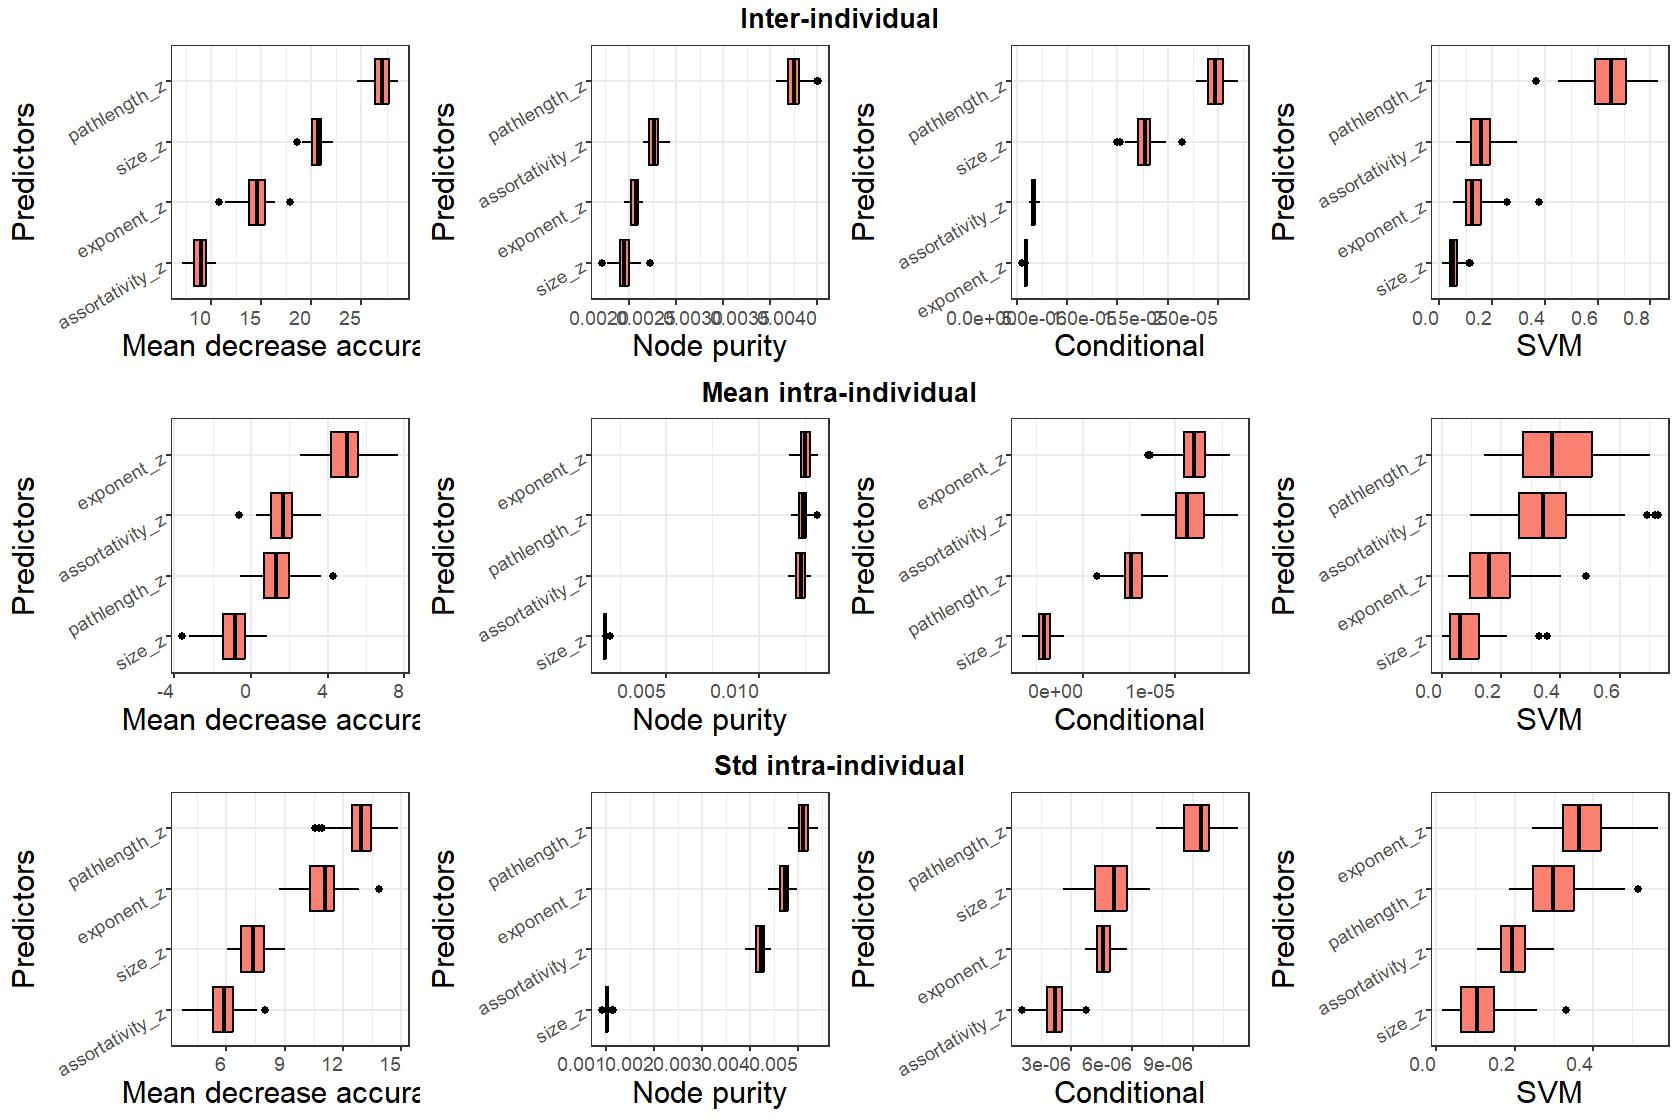
\includegraphics{./Figures/unnamed-chunk-103-1} 

}

\caption{Success in small-world networks in language change scenario for each type of method.}\label{fig:unnamed-chunk-103}
\end{figure}

\textbf{Predictor importance} in language change context:

Important: note that the metrics are printed by decreasing importance,
so their order may vary between the different methods!

\begin{figure}[!H]

{\centering 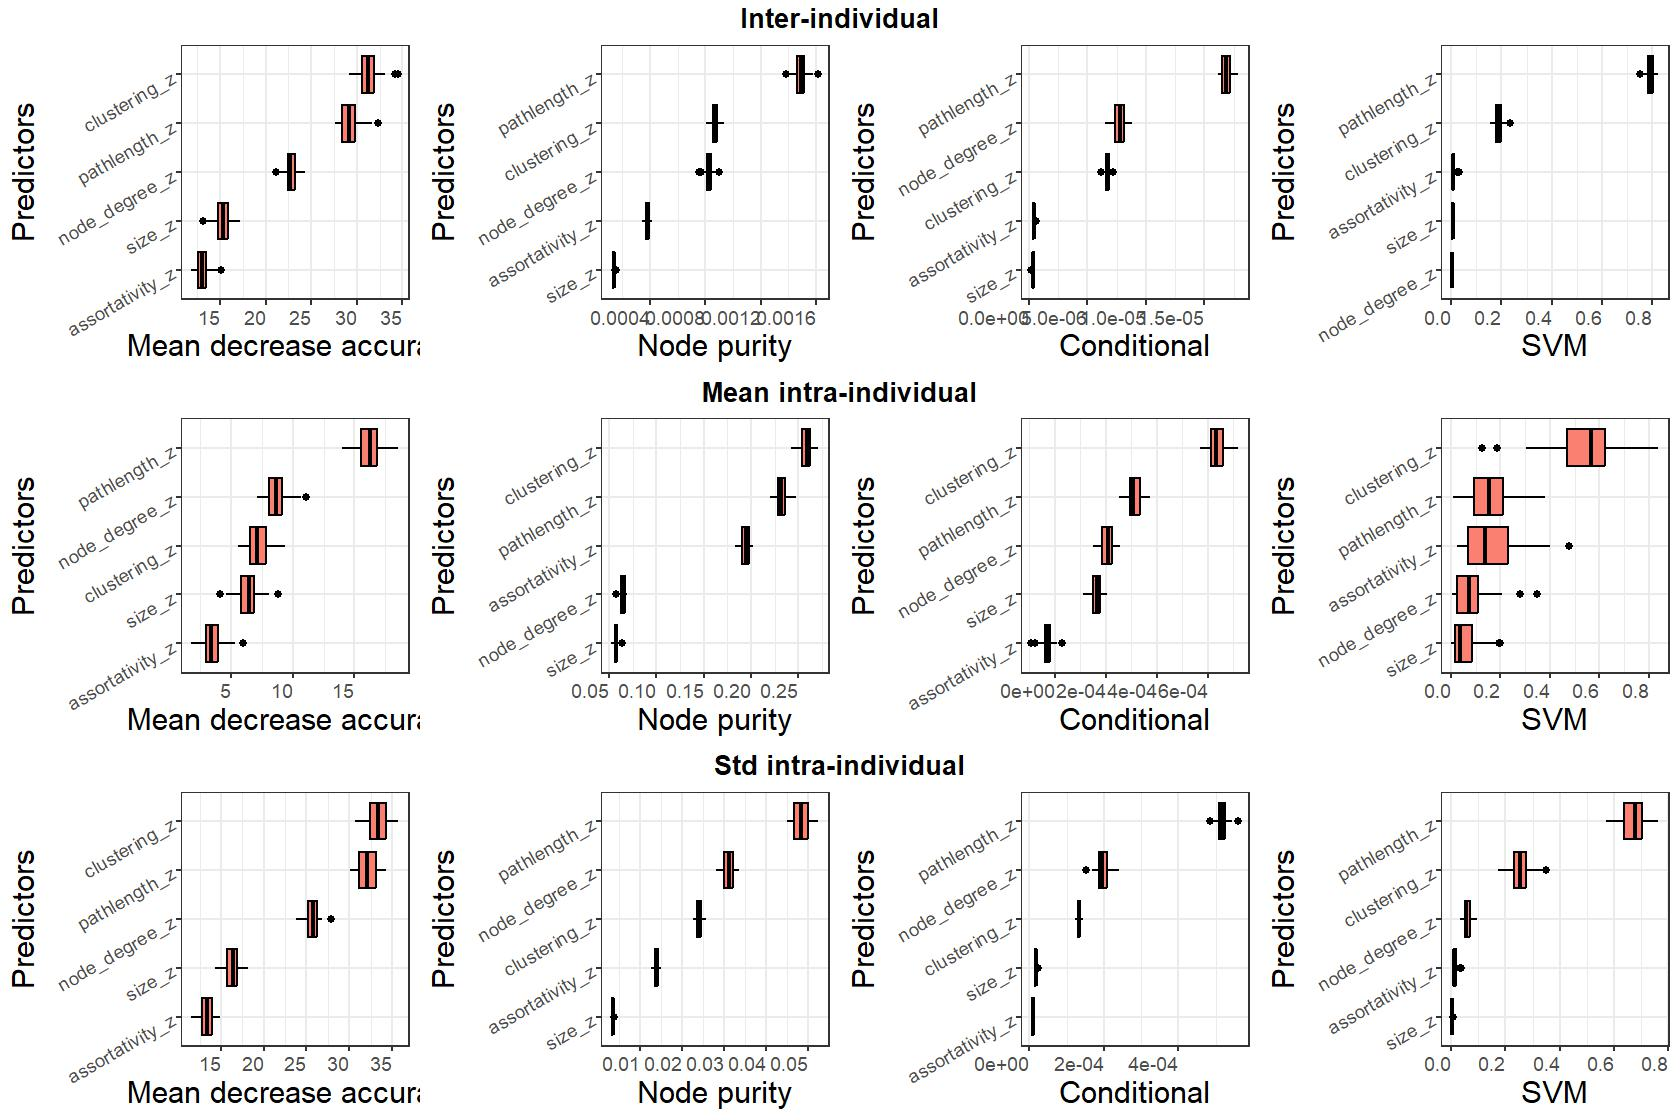
\includegraphics{./Figures/unnamed-chunk-104-1} 

}

\caption{Predictor importance in small-world networks in language change scenario for each type of method.}\label{fig:unnamed-chunk-104}
\end{figure}

\hypertarget{scale-free-networks}{%
\paragraph{Scale-free networks}\label{scale-free-networks}}

\textbf{Success} in language \textbf{emergence} context:

\emph{Inter-individual variation}:

\begin{itemize}
\tightlist
\item
  random forests: R\textsuperscript{2} = 37.5\% ±0.4\%, RMSE = 0.006
  ±0.000
\item
  conditional random forests: R\textsuperscript{2} = 55.8\% ±0.2\%, RMSE
  = 0.005 ±0.000.
\item
  support vector machines: R\textsuperscript{2} = 37.5\% ±9.3\%, RMSE =
  0.006 ±0.000.
\end{itemize}

\emph{Mean Intra-individual variation}:

\begin{itemize}
\tightlist
\item
  random forests: R\textsuperscript{2} = 1.7\% ±0.3\%, RMSE = 0.016
  ±0.000
\item
  conditional random forests: R\textsuperscript{2} = 34.5\% ±0.7\%, RMSE
  = 0.014 ±0.000.
\item
  support vector machines: R\textsuperscript{2} = 4.1\% ±5.6\%, RMSE =
  0.016 ±0.002.
\end{itemize}

\emph{Std Intra-individual variation}:

\begin{itemize}
\tightlist
\item
  random forests: R\textsuperscript{2} = 4.2\% ±0.4\%, RMSE = 0.010
  ±0.000
\item
  conditional random forests: R\textsuperscript{2} = 35.2\% ±0.5\%, RMSE
  = 0.008 ±0.000.
\item
  support vector machines: R\textsuperscript{2} = 11.1\% ±8.5\%, RMSE =
  0.009 ±0.001.
\end{itemize}

\begin{figure}[!H]

{\centering 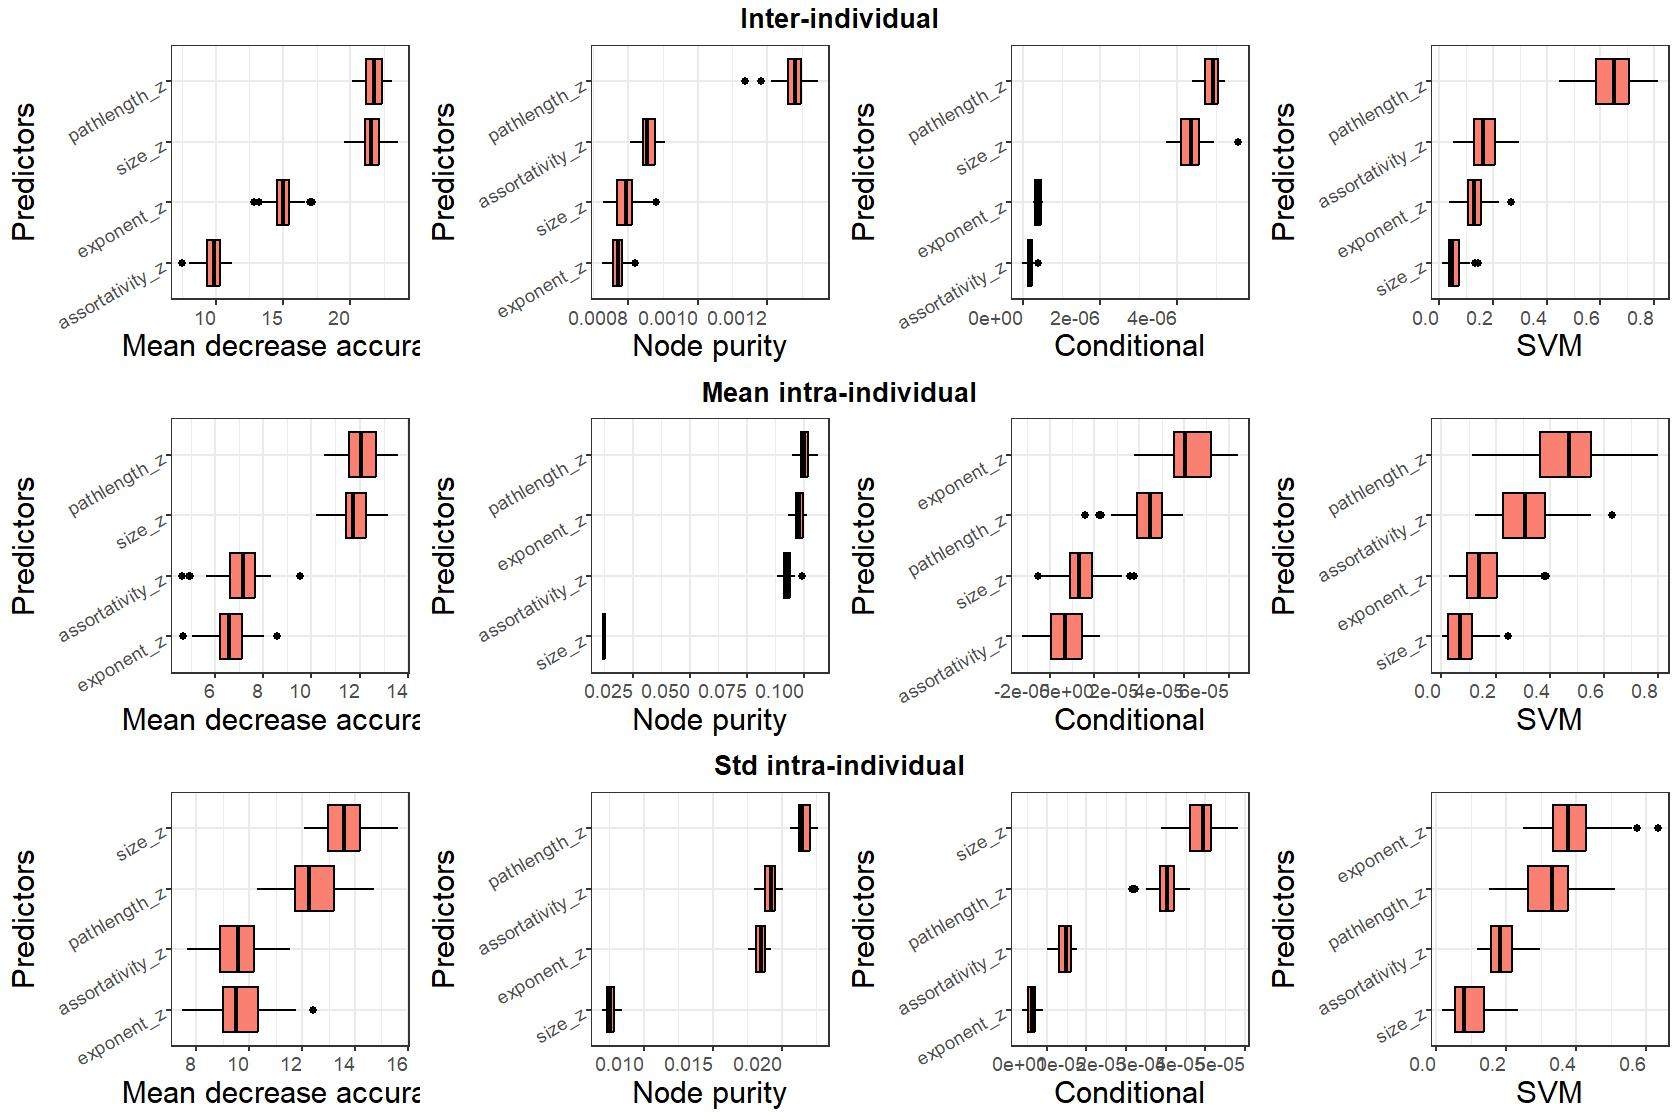
\includegraphics{./Figures/unnamed-chunk-106-1} 

}

\caption{Success (using R² and RMSE indexes) in scale-free networks in language emergence scenario for each type of method.}\label{fig:unnamed-chunk-106}
\end{figure}

\textbf{Predictor importance} in language emergence context:

And now, let's visualize the importance of the predictors. Important:
note that the metrics are printed by decreasing importance, so their
order may vary between the different methods!

\begin{figure}[!H]

{\centering 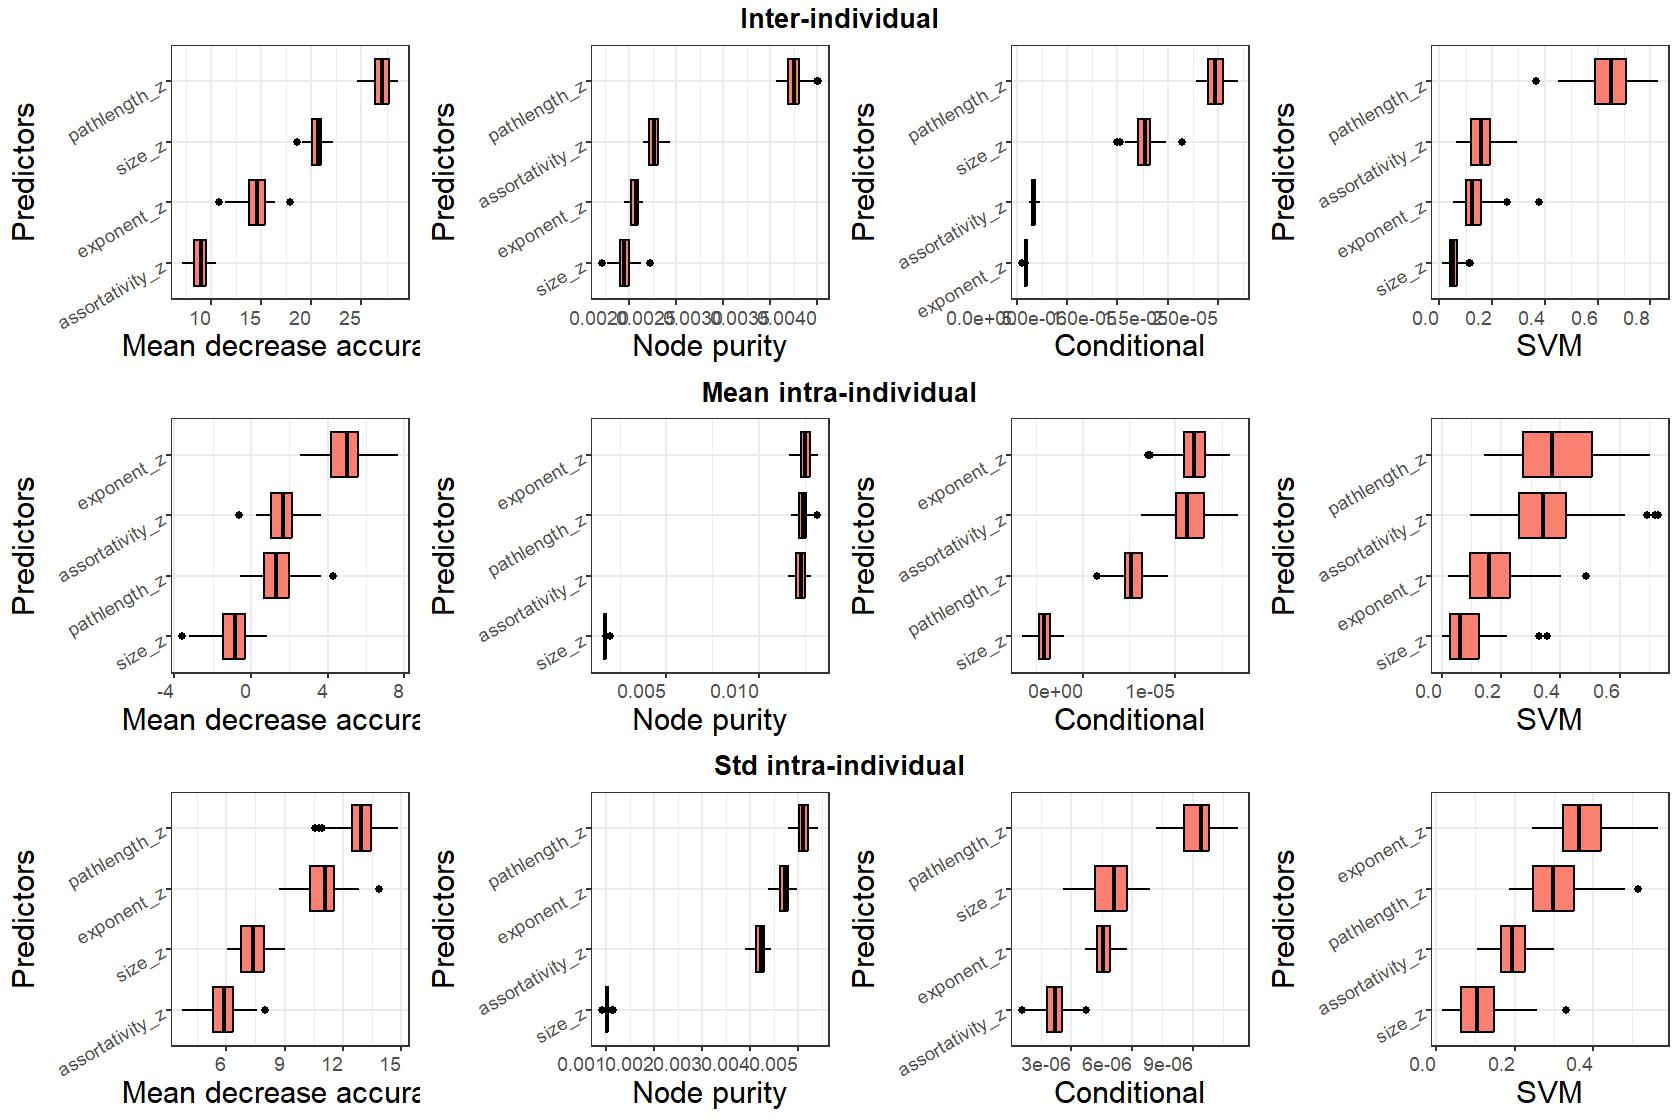
\includegraphics{./Figures/unnamed-chunk-107-1} 

}

\caption{Predictor importance in scale-free networks in language emergence scenario for each type of method.}\label{fig:unnamed-chunk-107}
\end{figure}

\textbf{Success} in language \textbf{change} context:

\emph{Inter-individual variation}:

\begin{itemize}
\tightlist
\item
  random forests: R\textsuperscript{2} = 36.8\% ±0.4\%, RMSE = 0.003
  ±0.000
\item
  conditional random forests: R\textsuperscript{2} = 54.5\% ±0.2\%, RMSE
  = 0.003 ±0.000.
\item
  support vector machines: R\textsuperscript{2} = 39.8\% ±8.4\%, RMSE =
  0.006 ±0.000.
\end{itemize}

\emph{Mean Intra-individual variation}:

\begin{itemize}
\tightlist
\item
  random forests: R\textsuperscript{2} = 0.0\% ±0.0\%, RMSE = 0.047
  ±0.000
\item
  conditional random forests: R\textsuperscript{2} = 36.4\% ±0.9\%, RMSE
  = 0.040 ±0.000.
\item
  support vector machines: R\textsuperscript{2} = 5.2\% ±4.8\%, RMSE =
  0.016 ±0.002.
\end{itemize}

\emph{Std Intra-individual variation}:

\begin{itemize}
\tightlist
\item
  random forests: R\textsuperscript{2} = 7.4\% ±0.4\%, RMSE = 0.019
  ±0.000
\item
  conditional random forests: R\textsuperscript{2} = 31.5\% ±0.3\%, RMSE
  = 0.017 ±0.000.
\item
  support vector machines: R\textsuperscript{2} = 11.4\% ±7.5\%, RMSE =
  0.009 ±0.001.
\end{itemize}

\begin{figure}[!H]

{\centering 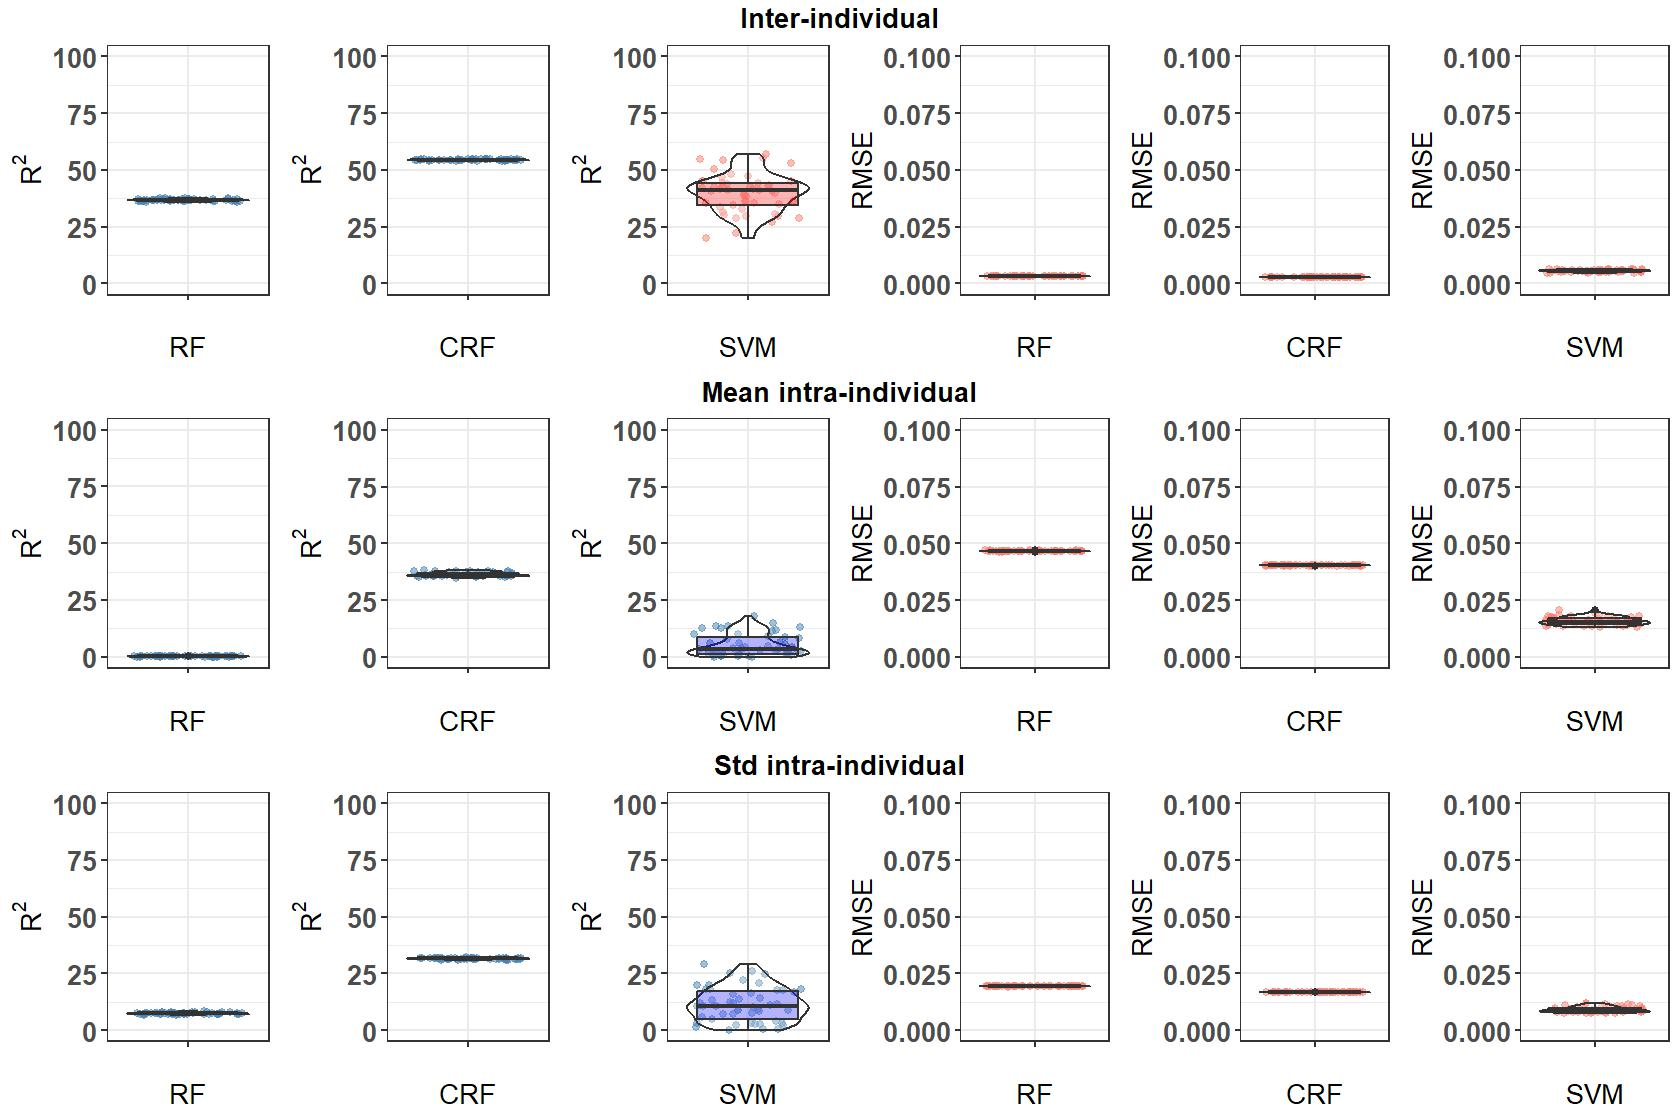
\includegraphics{./Figures/unnamed-chunk-109-1} 

}

\caption{Success (using R² and RMSE indexes) in scale-free networks in language change scenario for each type of method.}\label{fig:unnamed-chunk-109}
\end{figure}

\textbf{Predictor importance} in language change context:

Important: note that the metrics are printed by decreasing importance,
so their order may vary between the different methods!

\begin{figure}[!H]

{\centering 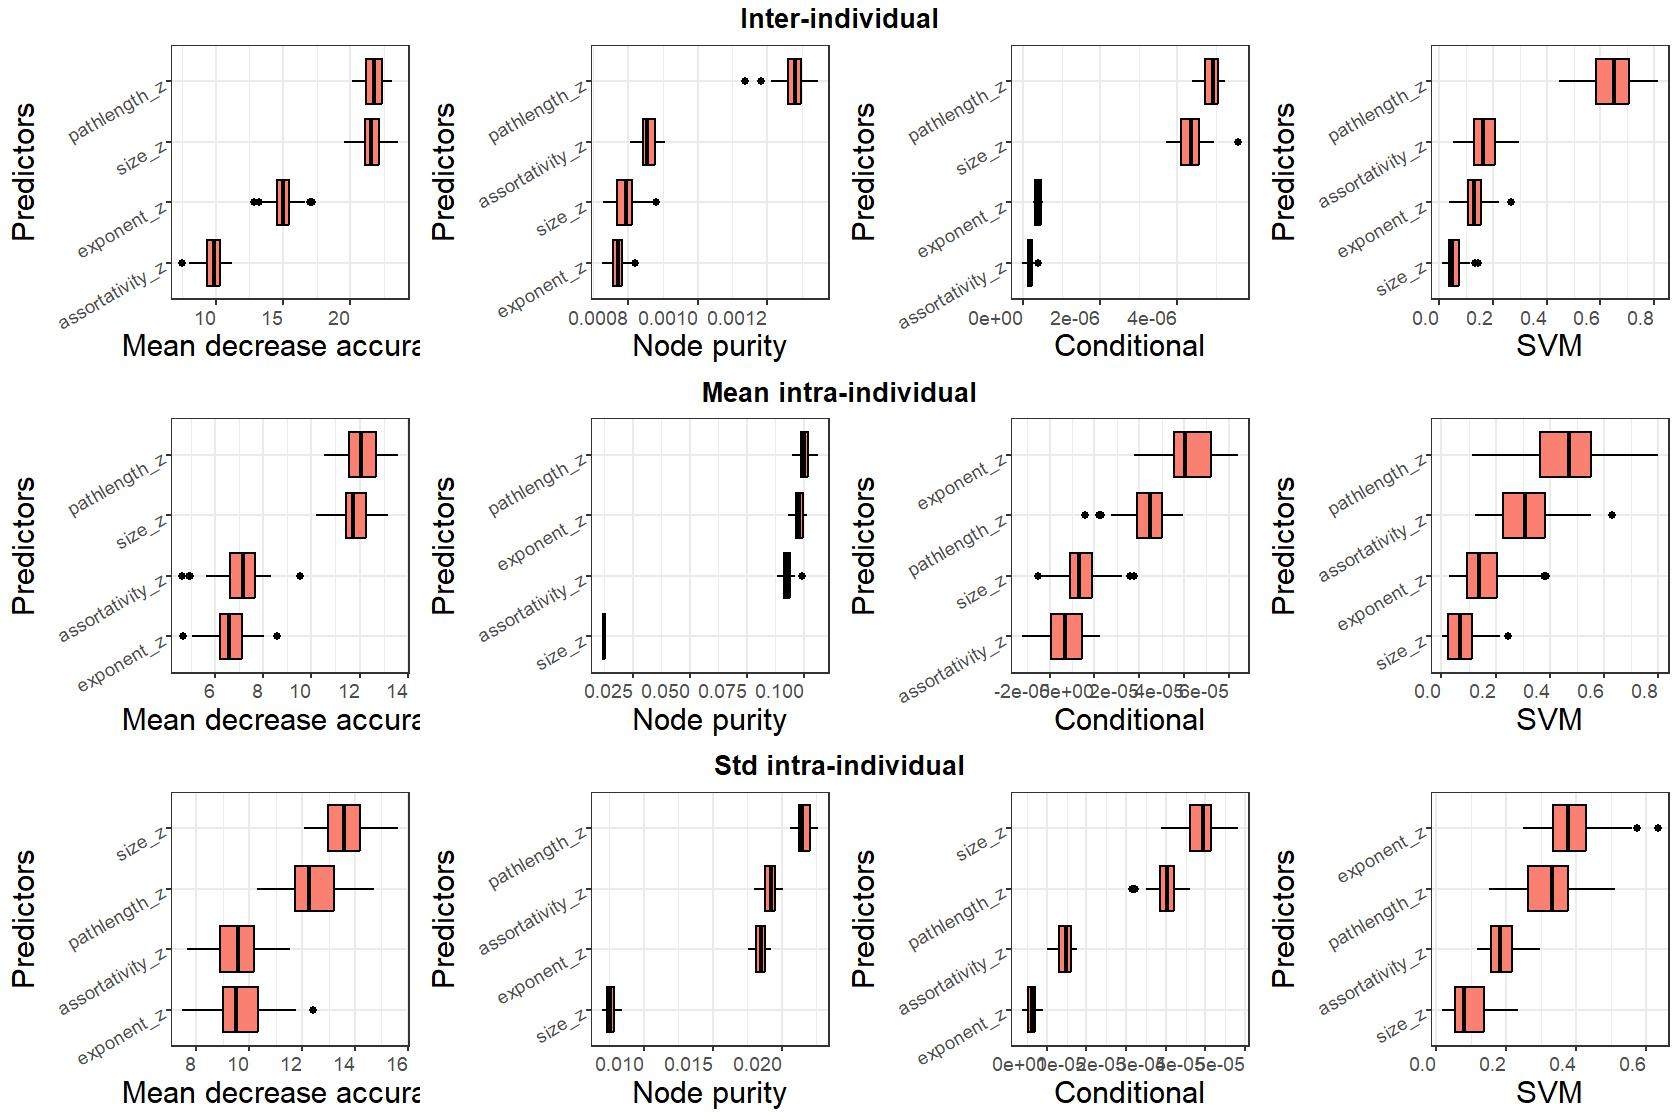
\includegraphics{./Figures/unnamed-chunk-110-1} 

}

\caption{Predictor importance in scale-free networks in language change scenario for each type of method.}\label{fig:unnamed-chunk-110}
\end{figure}

\hypertarget{summary-all}{%
\paragraph{Summary all}\label{summary-all}}

\textbf{Success}:

In language \emph{emergence} scenario:

\begin{longtable}[]{@{}lrrr@{}}
\toprule()
& Inter & Mintra & Sintra \\
\midrule()
\endhead
Random & 91.48819 & 45.324598 & 76.260186 \\
Small-World & 90.20976 & 58.875546 & 81.583876 \\
Scale-free & 37.50218 & 1.723138 & 4.176135 \\
\bottomrule()
\end{longtable}

In language \emph{change} scenario:

\begin{longtable}[]{@{}lrrr@{}}
\toprule()
& Inter & Mintra & Sintra \\
\midrule()
\endhead
Random & 95.86643 & 2.4651129 & 90.334545 \\
Small-World & 88.03344 & 4.6870283 & 82.062926 \\
Scale-free & 36.76559 & 0.0151357 & 7.401045 \\
\bottomrule()
\end{longtable}

The R² values are particularly low for intra-individual variation:
35.31\% on average for all types of networks in language emergence and
2.39\% for language change.

The R² values are also particularly low for scale-free variation: for
both language emergence and language change, it predicts 37.5\% for
inter-individual variation and 4.18\% for standard-deviation of
intra-individual variation.

The rest is well-predicted: The mean R² of inter-individual variation
for language emergence and change in random and small-world network is
of 91.49\%, while the standard-deviation of the intra-individual
variation is of 76.26\%.

\textbf{Predictor importance:}

Plot for the paper:

\begin{figure}[!H]

{\centering 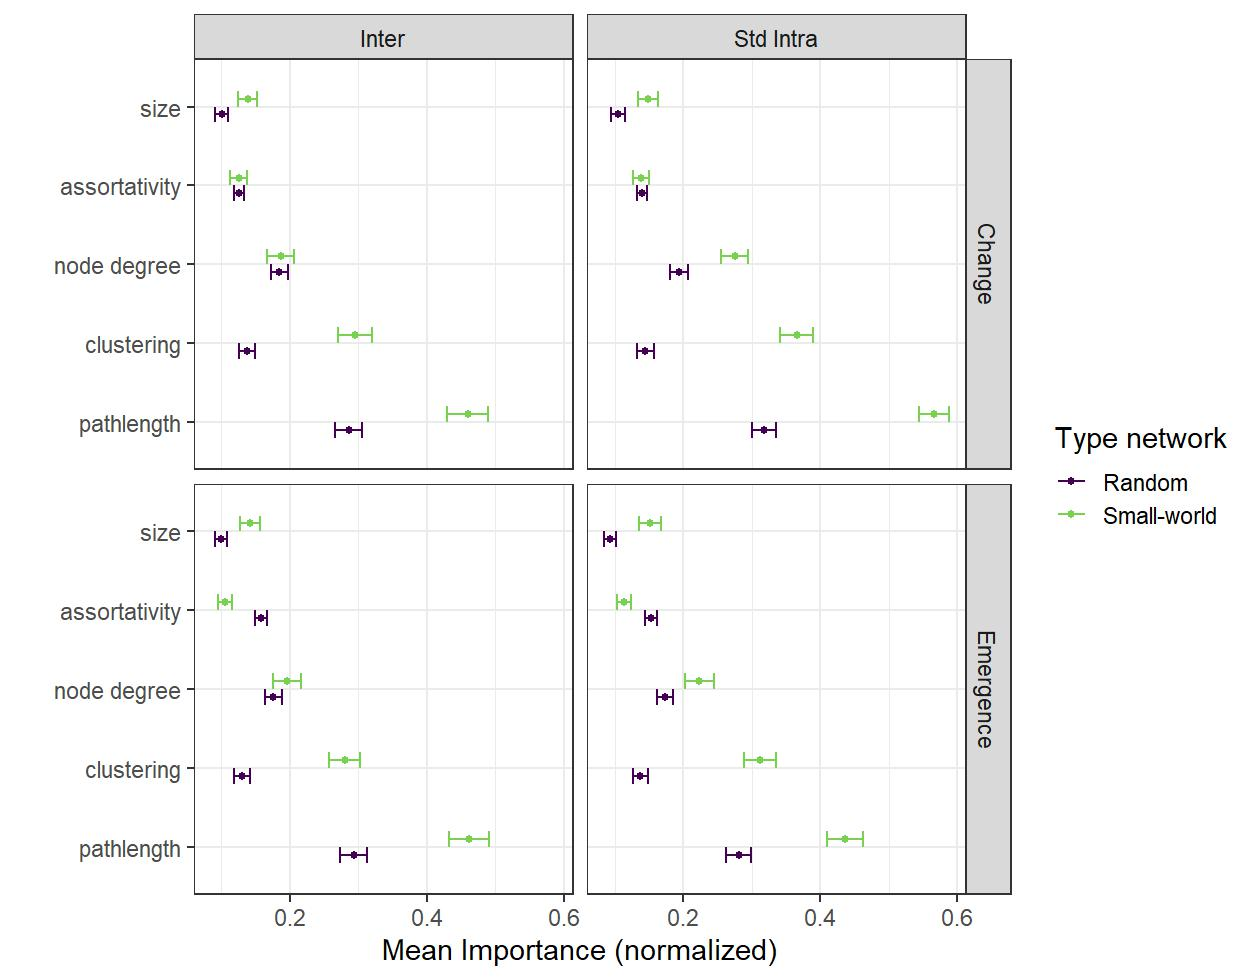
\includegraphics{./Figures/unnamed-chunk-115-1} 

}

\caption{Mean normalized predictor importance (mean of the four index including the accuracy-based and gini indexes from random forests, the index from conditional forests and the index from SVM) in random et small-world networks. We look at inter-individual variation (left panel) and standard-deviation of intra-individual variation (right panel) in language change scenario (upper panel) and language emergence scenario (lower panel). Note that we selected only the models with high success of prediction.}\label{fig:unnamed-chunk-115}
\end{figure}

Plot with all data:

\begin{figure}[!H]

{\centering \includegraphics{./Figures/unnamed-chunk-116-1} 

}

\caption{Mean normalized predictor importance (mean of the four index including the accuracy-based and gini indexes from random forests, the index from conditional forests and the index from SVM) in random, small-world et scale-fre networks. We look at inter-individual variation (left panel), mean intra-individual variation (middle panel) and standard-deviation of intra-individual variation (right panel) in language change scenario (upper panel) and language emergence scenario (lower panel)}\label{fig:unnamed-chunk-116}
\end{figure}

\begin{itemize}
\tightlist
\item
  Clearly, \emph{pathlength} is the best predictor for inter-individual
  and standard-deviation of intra-individual variation. It is followed
  by \emph{clustering coefficient}, and then \emph{node degree}.
\item
  None of the predictors accurately predict the mean intra-individual
  variation.
\item
  A similar pattern as for inter-individual variation emerges for the
  standard-deviation of intra-individual variation.
\end{itemize}

These results only concerns the machine learning techniques. They are
corrobated by the use of linear models (see part below, or go directly
to \protect\hyperlink{summary-modeling-part}{Summary Modeling part} for
a summary).

\hypertarget{modeling}{%
\subsubsection{Modeling}\label{modeling}}

Then, we wish to observe the effect size of our different metrics using
modeling. In our models, we want to investigate the relative effect of
the different \emph{predictors} (here, our metrics normalized) on
\emph{variation} (our different measures for inter- and intra-
individual variability). Our measure of variation are all
\emph{continuous}, so we use a \emph{linear model} with function
\texttt{lm} (stats package, version 3.6.2, see
\href{https://www.rdocumentation.org/packages/stats/versions/3.6.2/topics/lm}{here}
for more information).

\hypertarget{controling-for-vif}{%
\paragraph{Controling for VIF}\label{controling-for-vif}}

To do so, we create a model including all metrics as predictors. Then,
using this model, we first look at the \textbf{VIF score} (Variance
Inflation Factor). In statistics, the VIF score shows the extent of
multicollinearity in a regression analysis. It is \emph{``the ratio
(quotient) of the variance of estimating some parameter in a model that
includes multiple other terms (parameters) by the variance of a model
constructed using only one terms.''}.

The extent to which a VIF score is ``too high'' is still debated. In
general, it is suggested that a VIF score greater than 5 reflects highly
correlated predictors (source:
\href{https://www.statisticshowto.com/variance-inflation-factor/}{here}
or
\href{https://www.isixsigma.com/dictionary/variance-inflation-factor-vif/}{here}),
but please note that there is no absolute ``truth'' for what is a high
VIF score.

In \textbf{scale-free networks}:

In language \emph{emergence}:

\begin{longtable}[]{@{}lr@{}}
\toprule()
metrics & vif\_score \\
\midrule()
\endhead
exponent\_z & 2.094996 \\
assortativity\_z & 2.176258 \\
pathlength\_z & 3.122374 \\
size\_z & 4.559353 \\
\bottomrule()
\end{longtable}

In language \emph{change}:

\begin{longtable}[]{@{}lr@{}}
\toprule()
metrics & vif\_score \\
\midrule()
\endhead
exponent\_z & 2.232382 \\
assortativity\_z & 2.052236 \\
pathlength\_z & 2.936720 \\
size\_z & 5.012959 \\
\bottomrule()
\end{longtable}

We observe that no metrics have a VIF too high (above 5). Thus, we will
keep all metrics in the model of scale-free networks.

In \textbf{small-world networks}:

In language \emph{emergence}:

\begin{longtable}[]{@{}lr@{}}
\toprule()
metrics & vif\_score \\
\midrule()
\endhead
clustering\_z & 2.212031 \\
node\_degree\_z & 3.581759 \\
size\_z & 2.056694 \\
assortativity\_z & 1.254807 \\
pathlength\_z & 2.819969 \\
\bottomrule()
\end{longtable}

In language \emph{change}:

\begin{longtable}[]{@{}lr@{}}
\toprule()
metrics & vif\_score \\
\midrule()
\endhead
clustering\_z & 2.256314 \\
node\_degree\_z & 3.630869 \\
size\_z & 2.105092 \\
assortativity\_z & 1.253142 \\
pathlength\_z & 3.021626 \\
\bottomrule()
\end{longtable}

We observe that no metrics have a VIF too high (above 5). Thus, we will
keep all metrics in the model of small-world networks.

In \textbf{random networks}:

In language \emph{emergence}:

\begin{longtable}[]{@{}lr@{}}
\toprule()
metrics & vif\_score \\
\midrule()
\endhead
node\_degree\_z & 7.368530 \\
size\_z & 4.821028 \\
clustering\_z & 7.776622 \\
pathlength\_z & 3.560723 \\
assortativity\_z & 1.380199 \\
\bottomrule()
\end{longtable}

In language \emph{change}:

\begin{longtable}[]{@{}lr@{}}
\toprule()
metrics & vif\_score \\
\midrule()
\endhead
node\_degree\_z & 7.450035 \\
size\_z & 5.433643 \\
clustering\_z & 7.624188 \\
pathlength\_z & 3.393699 \\
assortativity\_z & 1.581143 \\
\bottomrule()
\end{longtable}

We observe that the following metrics have a VIF too high (above 5):
\emph{clustering} and \emph{node degree}. However, the VIF score is not
that much higher than 5 (7 for both metrics). To check which of these
two metrics explains the most variation, we create models using only the
two metrics (for both inter- and intra- individual variation):

\begin{verbatim}

Call:
lm(formula = inter_var * 100 ~ clustering_z + node_degree_z, 
    data = subdf_mod_ran_em)

Residuals:
     Min       1Q   Median       3Q      Max 
-0.17264 -0.10718 -0.03745  0.02481  1.77137 

Coefficients:
               Estimate Std. Error t value Pr(>|t|)    
(Intercept)    0.051867   0.014481   3.582 0.000399 ***
clustering_z  -0.081600   0.018601  -4.387  1.6e-05 ***
node_degree_z -0.003229   0.018555  -0.174 0.861982    
---
Signif. codes:  0 '***' 0.001 '**' 0.01 '*' 0.05 '.' 0.1 ' ' 1

Residual standard error: 0.2504 on 296 degrees of freedom
Multiple R-squared:  0.1006,    Adjusted R-squared:  0.0945 
F-statistic: 16.55 on 2 and 296 DF,  p-value: 1.536e-07
\end{verbatim}

\begin{verbatim}

Call:
lm(formula = mean_intra_var * 100 ~ clustering_z + node_degree_z, 
    data = subdf_mod_ran_em)

Residuals:
     Min       1Q   Median       3Q      Max 
-19.1812  -1.3586   0.2887   1.8521   8.1046 

Coefficients:
              Estimate Std. Error t value Pr(>|t|)    
(Intercept)   225.4401     0.1694 1330.79   <2e-16 ***
clustering_z   -2.7810     0.2176  -12.78   <2e-16 ***
node_degree_z   3.0115     0.2171   13.87   <2e-16 ***
---
Signif. codes:  0 '***' 0.001 '**' 0.01 '*' 0.05 '.' 0.1 ' ' 1

Residual standard error: 2.929 on 296 degrees of freedom
Multiple R-squared:  0.4268,    Adjusted R-squared:  0.4229 
F-statistic: 110.2 on 2 and 296 DF,  p-value: < 2.2e-16
\end{verbatim}

\begin{verbatim}

Call:
lm(formula = std_intra_var * 100 ~ clustering_z + node_degree_z, 
    data = subdf_mod_ran_em)

Residuals:
    Min      1Q  Median      3Q     Max 
-0.4323 -0.2181 -0.0823  0.0686  6.0083 

Coefficients:
              Estimate Std. Error t value Pr(>|t|)    
(Intercept)    0.17475    0.03273   5.339 1.86e-07 ***
clustering_z  -0.19301    0.04204  -4.591 6.54e-06 ***
node_degree_z -0.03476    0.04194  -0.829    0.408    
---
Signif. codes:  0 '***' 0.001 '**' 0.01 '*' 0.05 '.' 0.1 ' ' 1

Residual standard error: 0.566 on 296 degrees of freedom
Multiple R-squared:  0.1278,    Adjusted R-squared:  0.1219 
F-statistic: 21.69 on 2 and 296 DF,  p-value: 1.623e-09
\end{verbatim}

We also did create models using only one predictor and looking at the
amount of variation (R-squared) it explains, but it yield to the same
conclusions: clearly, it seems that the \emph{clustering} coefficient
explains \emph{more} variation than the node degree. Since the VIF is
not that much higher than 5 and since this cutoff is arbitrary, we will
first use a model containing all predictors, to ensure coherence with
scale-free and small-world networks. At the end of the analysis, we will
also remove node degree from the predictors, to make sure that this is
does not affect our conclusions.

\textbf{Summary}

\begin{itemize}
\tightlist
\item
  In scale-free and small-world networks, we keep all predictors in the
  model, since the VIF is lower than 5 for all metrics.
\item
  In random networks, to ensure conherence with scale-free and
  small-world networks, we will still analyse a model with all
  predictors. However, our analysis suggest that clustering coefficient
  explains more variation than node degree.
\end{itemize}

\hypertarget{controlling-for-other-assumptions-of-linear-models}{%
\paragraph{Controlling for other assumptions of linear
models}\label{controlling-for-other-assumptions-of-linear-models}}

Here, we observe the diagnostic plots for all type of networks. Since
the diagnostic plots for \emph{language change} are extremely similar
with the diagnostic plots for \emph{language emergence} scenario, we
present here the plots only for language emergence.

\textbf{Random Networks}:

In language \emph{emergence} scenario:

\begin{figure}[!H]

{\centering \includegraphics{./Figures/unnamed-chunk-124-1} 

}

\caption{Diagnostic plots when predicting **inter**-individual variation (random networks, language emergence).}\label{fig:unnamed-chunk-124}
\end{figure}

\begin{figure}[!H]

{\centering \includegraphics{./Figures/unnamed-chunk-125-1} 

}

\caption{Diagnostic plots when predicting **mean intra**-individual variation (random networks, language emergence)}\label{fig:unnamed-chunk-125}
\end{figure}

\begin{figure}[!H]

{\centering \includegraphics{./Figures/unnamed-chunk-126-1} 

}

\caption{Diagnostic plots when predicting **standard-deviation of intra**-individual variation (random networks, language emergence)}\label{fig:unnamed-chunk-126}
\end{figure}

The model's assumptions are not being met. Below, we will attempt to
address this issue. Given the analogous patterns observed in both
language emergence and language change scenarios, we will focus on
correcting the model assumptions specifically in the context of language
emergence and inter-individual variation to assess its impact.

\begin{enumerate}
\def\labelenumi{\arabic{enumi}.}
\tightlist
\item
  Checking \emph{linearity} assumptions (residuals vs fitted, first
  plot)
\end{enumerate}

It seems that linearity is not respected. Thus, we also check whether a
quadratic model of these variables would fit better.

\begin{verbatim}

Call:
lm(formula = inter_var ~ size_z + clustering_z + I(clustering_z^2) + 
    node_degree_z + I(node_degree_z^2) + pathlength_z + I(pathlength_z^2) + 
    assortativity_z + I(assortativity_z^2), data = subdf_mod_ran_ch)

Residuals:
       Min         1Q     Median         3Q        Max 
-9.405e-04 -1.363e-05  3.360e-06  2.629e-05  1.777e-03 

Coefficients:
                       Estimate Std. Error t value Pr(>|t|)    
(Intercept)          -2.858e-04  3.085e-05  -9.264  < 2e-16 ***
size_z               -5.751e-05  3.422e-05  -1.680  0.09397 .  
clustering_z         -8.792e-04  7.195e-05 -12.220  < 2e-16 ***
I(clustering_z^2)    -1.685e-04  2.040e-05  -8.259 5.39e-15 ***
node_degree_z         1.362e-04  5.680e-05   2.397  0.01715 *  
I(node_degree_z^2)   -3.356e-05  1.701e-05  -1.974  0.04939 *  
pathlength_z         -1.355e-03  9.933e-05 -13.645  < 2e-16 ***
I(pathlength_z^2)     8.092e-04  1.882e-05  42.992  < 2e-16 ***
assortativity_z      -5.673e-05  1.944e-05  -2.919  0.00379 ** 
I(assortativity_z^2)  4.255e-05  6.870e-06   6.194 2.02e-09 ***
---
Signif. codes:  0 '***' 0.001 '**' 0.01 '*' 0.05 '.' 0.1 ' ' 1

Residual standard error: 0.0001975 on 288 degrees of freedom
Multiple R-squared:  0.9882,    Adjusted R-squared:  0.9879 
F-statistic:  2684 on 9 and 288 DF,  p-value: < 2.2e-16
\end{verbatim}

\begin{center}\includegraphics{./Figures/unnamed-chunk-127-1} \end{center}

It does not change much the results, and linearity is still not
respected.

\begin{enumerate}
\def\labelenumi{\arabic{enumi}.}
\setcounter{enumi}{1}
\tightlist
\item
  Checking \emph{normality} (normal Q-Q, second plot)
\end{enumerate}

\begin{verbatim}

    Shapiro-Wilk normality test

data:  resid(model)
W = 0.45829, p-value < 2.2e-16
\end{verbatim}

Significantly different from a normal distribution.

\begin{enumerate}
\def\labelenumi{\arabic{enumi}.}
\setcounter{enumi}{2}
\tightlist
\item
  Checking for \emph{homoscedasticity} (scale-location, third plot)
\end{enumerate}

\begin{verbatim}
Non-constant Variance Score Test 
Variance formula: ~ fitted.values 
Chisquare = 2686.694, Df = 1, p = < 2.22e-16
\end{verbatim}

The data has clearly heteroscedasticity. We log the output to decrease
heteroscedasticity.

\begin{center}\includegraphics{./Figures/unnamed-chunk-130-1} \end{center}

\begin{verbatim}
Non-constant Variance Score Test 
Variance formula: ~ fitted.values 
Chisquare = 2.681535, Df = 1, p = 0.10152
\end{verbatim}

The data still has heteroscedasticity, but less.

\begin{enumerate}
\def\labelenumi{\arabic{enumi}.}
\setcounter{enumi}{3}
\tightlist
\item
  Checking the \emph{influence of extreme values} (Residuals versus
  Leverage, fourth plot).
\end{enumerate}

\textbf{scale-free Networks}:

In language \emph{emergence} scenario:

\begin{figure}[!H]

{\centering \includegraphics{./Figures/unnamed-chunk-131-1} 

}

\caption{Diagnostic plots when predicting **inter*-individual variation (scale-free networks, language emergence)}\label{fig:unnamed-chunk-131}
\end{figure}

\begin{figure}[!H]

{\centering \includegraphics{./Figures/unnamed-chunk-132-1} 

}

\caption{Diagnostic plots when predicting **mean intra**-individual variation (scale-free networks, language emergence)}\label{fig:unnamed-chunk-132}
\end{figure}

\begin{figure}[!H]

{\centering \includegraphics{./Figures/unnamed-chunk-133-1} 

}

\caption{Diagnostic plots when predicting **standard-deviation of intra**-individual variation (scale-free networks, language emergence)}\label{fig:unnamed-chunk-133}
\end{figure}

\textbf{Small-world Networks}:

In language \emph{emergence} scenario:

\begin{figure}[!H]

{\centering \includegraphics{./Figures/unnamed-chunk-134-1} 

}

\caption{Diagnostic plots when predicting **inter**-individual variation (small-world networks, language emergence)}\label{fig:unnamed-chunk-134}
\end{figure}

\begin{figure}[!H]

{\centering \includegraphics{./Figures/unnamed-chunk-135-1} 

}

\caption{Diagnostic plots when predicting **mean intra**-individual variation (small-world networks, language emergence)}\label{fig:unnamed-chunk-135}
\end{figure}

\begin{figure}[!H]

{\centering \includegraphics{./Figures/unnamed-chunk-136-1} 

}

\caption{Diagnostic plots when predicting **standard-deviation of intra**-individual variation (small-world networks, language emergence)}\label{fig:unnamed-chunk-136}
\end{figure}

\hypertarget{methodology-for-the-models}{%
\paragraph{Methodology for the
models}\label{methodology-for-the-models}}

First, we create a \textbf{linear model} using these metrics as
predictors and the type of variation (inter, mean intra, std intra) as
the predicted variable. For easier visualizuation, please note that we
multiply all types of variation by 100, in both language emergence and
language change scenarios. All predictors are z-scored.

\begin{enumerate}
\def\labelenumi{\arabic{enumi}.}
\item
  We first look at the \emph{summary} of \emph{each} linear models.
\item
  Then, we gather the \emph{standardized estimates} in a table.
\item
  We also use \emph{step models} (using \texttt{stats} package), which
  chooses a model by AIC in a stepwise Algorithm. The \emph{Akaike
  information criterion (AIC)} is an estimator of prediction error and
  thereby relative quality of statistical models for a given set of
  data. Given a collection of models for the data, AIC estimates the
  quality of each model, relative to each of the other models. Thus, AIC
  provides a means for model selection. Step models show the best
  predictors and also indicates the most important predictors for
  maximizing \textbf{AIC} (increasing importance). In other terms, it
  shows how much the AIC increases when removing a predictor from the
  model (the higher the AIC, the worst the model).
\item
  In order to look at the variable importance, we also integrate all
  variables in a model, then remove each of them to evaluate the
  decrease in the total R² of the model.
\item
  Finally, we create models with single predictors and evaluate the
  total R² that these predictors explain.
\end{enumerate}

\hypertarget{inter-individual-variation}{%
\paragraph{Inter-individual
variation}\label{inter-individual-variation}}

\textbf{1 - Summary of the linear models.}

For \emph{random} networks, in language \emph{emergence}:

\begin{verbatim}

Call:
lm(formula = inter_var * 100 ~ clustering_z + assortativity_z + 
    pathlength_z + size_z + node_degree_z, data = subdf_mod_ran_em)

Residuals:
     Min       1Q   Median       3Q      Max 
-0.38396 -0.01526  0.00626  0.03998  0.59269 

Coefficients:
                 Estimate Std. Error t value Pr(>|t|)    
(Intercept)      0.050242   0.005232   9.603  < 2e-16 ***
clustering_z     0.182628   0.014649  12.467  < 2e-16 ***
assortativity_z -0.015529   0.006194  -2.507  0.01271 *  
pathlength_z     0.363731   0.009888  36.785  < 2e-16 ***
size_z          -0.028448   0.011487  -2.477  0.01383 *  
node_degree_z    0.039037   0.014224   2.744  0.00644 ** 
---
Signif. codes:  0 '***' 0.001 '**' 0.01 '*' 0.05 '.' 0.1 ' ' 1

Residual standard error: 0.09046 on 293 degrees of freedom
Multiple R-squared:  0.8838,    Adjusted R-squared:  0.8818 
F-statistic: 445.7 on 5 and 293 DF,  p-value: < 2.2e-16
\end{verbatim}

For \emph{random} networks, in language \emph{change}:

\begin{verbatim}

Call:
lm(formula = inter_var * 100 ~ clustering_z + assortativity_z + 
    pathlength_z + size_z + node_degree_z, data = subdf_mod_ran_ch)

Residuals:
      Min        1Q    Median        3Q       Max 
-0.252490 -0.011758  0.004671  0.027376  0.292066 

Coefficients:
                 Estimate Std. Error t value Pr(>|t|)    
(Intercept)      0.033849   0.003471   9.752  < 2e-16 ***
clustering_z     0.131623   0.009642  13.651  < 2e-16 ***
assortativity_z -0.015461   0.004422  -3.496 0.000545 ***
pathlength_z     0.250502   0.006404  39.120  < 2e-16 ***
size_z          -0.010637   0.008076  -1.317 0.188841    
node_degree_z    0.021007   0.009487   2.214 0.027587 *  
---
Signif. codes:  0 '***' 0.001 '**' 0.01 '*' 0.05 '.' 0.1 ' ' 1

Residual standard error: 0.0599 on 292 degrees of freedom
Multiple R-squared:  0.8902,    Adjusted R-squared:  0.8883 
F-statistic: 473.3 on 5 and 292 DF,  p-value: < 2.2e-16
\end{verbatim}

For \emph{small-world} networks, in language \emph{emergence}:

\begin{verbatim}

Call:
lm(formula = inter_var * 100 ~ clustering_z + assortativity_z + 
    pathlength_z + size_z + node_degree_z, data = subdf_mod_sw_em)

Residuals:
     Min       1Q   Median       3Q      Max 
-0.46288 -0.17581 -0.01208  0.13034  1.09315 

Coefficients:
                Estimate Std. Error t value Pr(>|t|)    
(Intercept)      0.35133    0.01400  25.103  < 2e-16 ***
clustering_z     0.22439    0.02085  10.762  < 2e-16 ***
assortativity_z  0.08090    0.01570   5.152 4.73e-07 ***
pathlength_z     0.68205    0.02354  28.972  < 2e-16 ***
size_z          -0.11873    0.02010  -5.905 9.70e-09 ***
node_degree_z    0.04566    0.02653   1.721   0.0863 .  
---
Signif. codes:  0 '***' 0.001 '**' 0.01 '*' 0.05 '.' 0.1 ' ' 1

Residual standard error: 0.2424 on 294 degrees of freedom
Multiple R-squared:  0.8479,    Adjusted R-squared:  0.8453 
F-statistic: 327.8 on 5 and 294 DF,  p-value: < 2.2e-16
\end{verbatim}

For \emph{small-world} networks, in language \emph{change}:

\begin{verbatim}

Call:
lm(formula = inter_var * 100 ~ clustering_z + assortativity_z + 
    pathlength_z + size_z + node_degree_z, data = subdf_mod_sw_ch)

Residuals:
     Min       1Q   Median       3Q      Max 
-0.30734 -0.11059 -0.00921  0.07822  1.00512 

Coefficients:
                 Estimate Std. Error t value Pr(>|t|)    
(Intercept)      0.236805   0.009445  25.072  < 2e-16 ***
clustering_z     0.140855   0.014211   9.912  < 2e-16 ***
assortativity_z  0.044994   0.010591   4.248 2.89e-05 ***
pathlength_z     0.420955   0.016445  25.597  < 2e-16 ***
size_z          -0.074567   0.013726  -5.432 1.17e-07 ***
node_degree_z    0.023018   0.018027   1.277    0.203    
---
Signif. codes:  0 '***' 0.001 '**' 0.01 '*' 0.05 '.' 0.1 ' ' 1

Residual standard error: 0.1636 on 294 degrees of freedom
Multiple R-squared:  0.8197,    Adjusted R-squared:  0.8167 
F-statistic: 267.4 on 5 and 294 DF,  p-value: < 2.2e-16
\end{verbatim}

For \emph{scale-free} networks, in language \emph{emergence}:

\begin{verbatim}

Call:
lm(formula = inter_var * 100 ~ exponent_z + assortativity_z + 
    pathlength_z + size_z, data = subdf_mod_sf_em)

Residuals:
     Min       1Q   Median       3Q      Max 
-1.47445 -0.33898 -0.01628  0.31736  1.61598 

Coefficients:
                Estimate Std. Error t value Pr(>|t|)    
(Intercept)      3.30238    0.03205 103.045  < 2e-16 ***
exponent_z      -0.07074    0.04646  -1.523  0.12894    
assortativity_z -0.01776    0.04736  -0.375  0.70791    
pathlength_z     0.32245    0.05672   5.685 3.15e-08 ***
size_z           0.18763    0.06854   2.737  0.00657 ** 
---
Signif. codes:  0 '***' 0.001 '**' 0.01 '*' 0.05 '.' 0.1 ' ' 1

Residual standard error: 0.5551 on 295 degrees of freedom
Multiple R-squared:  0.3867,    Adjusted R-squared:  0.3784 
F-statistic:  46.5 on 4 and 295 DF,  p-value: < 2.2e-16
\end{verbatim}

For \emph{scale-free} networks, in language \emph{change}:

\begin{verbatim}

Call:
lm(formula = inter_var * 100 ~ exponent_z + assortativity_z + 
    pathlength_z + size_z, data = subdf_mod_sf_ch)

Residuals:
     Min       1Q   Median       3Q      Max 
-0.76479 -0.21379 -0.01904  0.18163  1.69505 

Coefficients:
                 Estimate Std. Error t value Pr(>|t|)    
(Intercept)      2.035471   0.019081 106.673  < 2e-16 ***
exponent_z      -0.002603   0.028557  -0.091   0.9274    
assortativity_z  0.027438   0.027381   1.002   0.3171    
pathlength_z     0.187230   0.032754   5.716 2.67e-08 ***
size_z           0.072220   0.042794   1.688   0.0925 .  
---
Signif. codes:  0 '***' 0.001 '**' 0.01 '*' 0.05 '.' 0.1 ' ' 1

Residual standard error: 0.3305 on 295 degrees of freedom
Multiple R-squared:  0.3951,    Adjusted R-squared:  0.3869 
F-statistic: 48.18 on 4 and 295 DF,  p-value: < 2.2e-16
\end{verbatim}

\textbf{2 - Summary of the standardized estimates of the linear models.}

For easier visualization, the following table gathers the effect size,
in absolute value, rounded and ordered from the highest to the lowest,
for each network type.

In language \emph{emergence}:

\begin{longtable}[]{@{}lrrr@{}}
\toprule()
metrics & Random & SmallWorld & ScaleFree \\
\midrule()
\endhead
(Intercept) & 0.05 & 0.35 & 3.30 \\
assortativity & 0.02 & 0.08 & 0.02 \\
clustering & 0.18 & 0.22 & NA \\
exponent & NA & NA & 0.07 \\
node degree & 0.04 & 0.05 & NA \\
pathlength & 0.36 & 0.68 & 0.32 \\
size & 0.03 & 0.12 & 0.19 \\
\bottomrule()
\end{longtable}

In language \emph{change}:

\begin{longtable}[]{@{}lrrr@{}}
\toprule()
metrics & Random & SmallWorld & ScaleFree \\
\midrule()
\endhead
(Intercept) & 0.03 & 0.24 & 2.04 \\
assortativity & 0.02 & 0.04 & 0.03 \\
clustering & 0.13 & 0.14 & NA \\
exponent & NA & NA & 0.00 \\
node degree & 0.02 & 0.02 & NA \\
pathlength & 0.25 & 0.42 & 0.19 \\
size & 0.01 & 0.07 & 0.07 \\
\bottomrule()
\end{longtable}

\textbf{3 - Step models (looking at AIC).}

For \emph{random} networks, in language \emph{emergence}:

\begin{verbatim}
Start:  AIC=-1430.97
inter_var * 100 ~ clustering_z + assortativity_z + pathlength_z + 
    size_z + node_degree_z

                  Df Sum of Sq     RSS     AIC
<none>                          2.3976 -1431.0
- size_z           1    0.0502  2.4478 -1426.8
- assortativity_z  1    0.0514  2.4490 -1426.6
- node_degree_z    1    0.0616  2.4592 -1425.4
- clustering_z     1    1.2718  3.6694 -1305.7
- pathlength_z     1   11.0723 13.4699  -916.9
\end{verbatim}

\begin{verbatim}

Call:
lm(formula = inter_var * 100 ~ clustering_z + assortativity_z + 
    pathlength_z + size_z + node_degree_z, data = subdf_mod_ran_em)

Coefficients:
    (Intercept)     clustering_z  assortativity_z     pathlength_z  
        0.05024          0.18263         -0.01553          0.36373  
         size_z    node_degree_z  
       -0.02845          0.03904  
\end{verbatim}

For \emph{random} networks, in language \emph{change}:

\begin{verbatim}
Start:  AIC=-1671.8
inter_var * 100 ~ clustering_z + assortativity_z + pathlength_z + 
    size_z + node_degree_z

                  Df Sum of Sq    RSS     AIC
- size_z           1    0.0062 1.0541 -1672.0
<none>                         1.0479 -1671.8
- node_degree_z    1    0.0176 1.0654 -1668.8
- assortativity_z  1    0.0439 1.0917 -1661.6
- clustering_z     1    0.6688 1.7166 -1526.7
- pathlength_z     1    5.4917 6.5395 -1128.1

Step:  AIC=-1672.04
inter_var * 100 ~ clustering_z + assortativity_z + pathlength_z + 
    node_degree_z

                  Df Sum of Sq    RSS     AIC
<none>                         1.0541 -1672.0
- node_degree_z    1    0.0158 1.0699 -1669.6
- assortativity_z  1    0.0648 1.1189 -1656.3
- clustering_z     1    1.5305 2.5846 -1406.8
- pathlength_z     1    6.1628 7.2168 -1100.8
\end{verbatim}

\begin{verbatim}

Call:
lm(formula = inter_var * 100 ~ clustering_z + assortativity_z + 
    pathlength_z + node_degree_z, data = subdf_mod_ran_ch)

Coefficients:
    (Intercept)     clustering_z  assortativity_z     pathlength_z  
        0.03380          0.14061         -0.01754          0.25304  
  node_degree_z  
        0.01031  
\end{verbatim}

For \emph{small-world} networks, in language \emph{emergence}:

\begin{verbatim}
Start:  AIC=-844.33
inter_var * 100 ~ clustering_z + assortativity_z + pathlength_z + 
    size_z + node_degree_z

                  Df Sum of Sq    RSS     AIC
<none>                         17.276 -844.33
- node_degree_z    1     0.174 17.450 -843.33
- assortativity_z  1     1.560 18.836 -820.40
- size_z           1     2.049 19.326 -812.70
- clustering_z     1     6.806 24.082 -746.70
- pathlength_z     1    49.324 66.600 -441.52
\end{verbatim}

\begin{verbatim}

Call:
lm(formula = inter_var * 100 ~ clustering_z + assortativity_z + 
    pathlength_z + size_z + node_degree_z, data = subdf_mod_sw_em)

Coefficients:
    (Intercept)     clustering_z  assortativity_z     pathlength_z  
        0.35133          0.22439          0.08090          0.68205  
         size_z    node_degree_z  
       -0.11873          0.04566  
\end{verbatim}

For \emph{small-world} networks, in language \emph{change}:

\begin{verbatim}
Start:  AIC=-1080.3
inter_var * 100 ~ clustering_z + assortativity_z + pathlength_z + 
    size_z + node_degree_z

                  Df Sum of Sq     RSS      AIC
- node_degree_z    1    0.0436  7.9116 -1080.64
<none>                          7.8679 -1080.30
- assortativity_z  1    0.4830  8.3510 -1064.42
- size_z           1    0.7897  8.6577 -1053.60
- clustering_z     1    2.6292 10.4971  -995.80
- pathlength_z     1   17.5349 25.4028  -730.68

Step:  AIC=-1080.64
inter_var * 100 ~ clustering_z + assortativity_z + pathlength_z + 
    size_z

                  Df Sum of Sq    RSS      AIC
<none>                          7.912 -1080.64
- assortativity_z  1     0.462  8.373 -1065.62
- size_z           1     0.889  8.800 -1050.70
- clustering_z     1     4.906 12.817  -937.90
- pathlength_z     1    34.134 42.046  -581.51
\end{verbatim}

\begin{verbatim}

Call:
lm(formula = inter_var * 100 ~ clustering_z + assortativity_z + 
    pathlength_z + size_z, data = subdf_mod_sw_ch)

Coefficients:
    (Intercept)     clustering_z  assortativity_z     pathlength_z  
        0.23681          0.15198          0.04382          0.40577  
         size_z  
       -0.06439  
\end{verbatim}

For \emph{scale-free} networks, in language \emph{emergence}:

\begin{verbatim}
Start:  AIC=-348.22
inter_var * 100 ~ exponent_z + assortativity_z + pathlength_z + 
    size_z

                  Df Sum of Sq     RSS     AIC
- assortativity_z  1    0.0433  90.938 -350.08
<none>                          90.895 -348.22
- exponent_z       1    0.7143  91.609 -347.88
- size_z           1    2.3088  93.204 -342.70
- pathlength_z     1    9.9567 100.851 -319.04

Step:  AIC=-350.08
inter_var * 100 ~ exponent_z + pathlength_z + size_z

               Df Sum of Sq     RSS     AIC
<none>                       90.938 -350.08
- exponent_z    1    0.8760  91.814 -349.20
- size_z        1    2.2863  93.224 -344.63
- pathlength_z  1   10.0827 101.021 -320.54
\end{verbatim}

\begin{verbatim}

Call:
lm(formula = inter_var * 100 ~ exponent_z + pathlength_z + size_z, 
    data = subdf_mod_sf_em)

Coefficients:
 (Intercept)    exponent_z  pathlength_z        size_z  
     3.30238      -0.07544       0.31833       0.18174  
\end{verbatim}

For \emph{scale-free} networks, in language \emph{change}:

\begin{verbatim}
Start:  AIC=-659.33
inter_var * 100 ~ exponent_z + assortativity_z + pathlength_z + 
    size_z

                  Df Sum of Sq    RSS     AIC
- exponent_z       1    0.0009 32.224 -661.32
- assortativity_z  1    0.1097 32.333 -660.31
<none>                         32.223 -659.33
- size_z           1    0.3111 32.534 -658.45
- pathlength_z     1    3.5691 35.792 -629.82

Step:  AIC=-661.32
inter_var * 100 ~ assortativity_z + pathlength_z + size_z

                  Df Sum of Sq    RSS     AIC
- assortativity_z  1    0.1108 32.335 -662.29
<none>                         32.224 -661.32
- size_z           1    0.4046 32.628 -659.58
- pathlength_z     1    3.8345 36.058 -629.59

Step:  AIC=-662.29
inter_var * 100 ~ pathlength_z + size_z

               Df Sum of Sq    RSS     AIC
<none>                      32.335 -662.29
- size_z        1    0.8466 33.181 -656.54
- pathlength_z  1    3.8690 36.204 -630.39
\end{verbatim}

\begin{verbatim}

Call:
lm(formula = inter_var * 100 ~ pathlength_z + size_z, data = subdf_mod_sf_ch)

Coefficients:
 (Intercept)  pathlength_z        size_z  
      2.0355        0.1888        0.0883  
\end{verbatim}

\textbf{4 - Drop in R² when removing predictors}

Language \emph{emergence}:

\begin{longtable}[]{@{}lrrr@{}}
\toprule()
term & Random & SmallWorld & ScaleFree \\
\midrule()
\endhead
clustering & 0.0616377 & 0.0599168 & NA \\
node\_degree & 0.0029870 & 0.0015321 & NA \\
assortativity & 0.0024929 & 0.0137317 & 0.0002924 \\
pathlength & 0.5366329 & 0.4342481 & 0.0671823 \\
size & 0.0024325 & 0.0180421 & 0.0155788 \\
exponent & NA & NA & 0.0048196 \\
\bottomrule()
\end{longtable}

Language \emph{change}:

\begin{longtable}[]{@{}lrrr@{}}
\toprule()
term & Random & SmallWorld & ScaleFree \\
\midrule()
\endhead
clustering & 0.0701024 & 0.0602336 & NA \\
node\_degree & 0.0018442 & 0.0009996 & NA \\
assortativity & 0.0045983 & 0.0110663 & 0.0020589 \\
pathlength & 0.5756553 & 0.4017201 & 0.0669968 \\
size & 0.0006525 & 0.0180929 & 0.0058397 \\
exponent & NA & NA & 0.0000170 \\
\bottomrule()
\end{longtable}

\textbf{5 - R² explained by each predictor}

Language \emph{emergence}:

\begin{longtable}[]{@{}lrrr@{}}
\toprule()
term & Random & SmallWorld & ScaleFree \\
\midrule()
\endhead
clustering & 0.0974584 & -0.0014516 & NA \\
node\_degree & 0.0388764 & 0.1682322 & NA \\
assortativity & 0.1480515 & -0.0032237 & 0.1495115 \\
pathlength & 0.6182816 & 0.6401498 & 0.3687975 \\
size & 0.0413732 & 0.0136092 & 0.3018147 \\
exponent & NA & NA & 0.0824252 \\
\bottomrule()
\end{longtable}

Language \emph{change}:

\begin{longtable}[]{@{}lrrr@{}}
\toprule()
term & Random & SmallWorld & ScaleFree \\
\midrule()
\endhead
clustering & 0.0998072 & -0.0027987 & NA \\
node\_degree & 0.0398155 & 0.1896333 & NA \\
assortativity & 0.1463084 & 0.0048742 & 0.1841091 \\
pathlength & 0.6218682 & 0.6223793 & 0.3750539 \\
size & 0.0418832 & 0.0092948 & 0.3181298 \\
exponent & NA & NA & 0.1261277 \\
\bottomrule()
\end{longtable}

\hypertarget{mean-intra-individual-variation}{%
\paragraph{Mean intra-individual
variation}\label{mean-intra-individual-variation}}

We apply here exactly the same steps, but using the mean
intra-individual variation as the predicted variable. Please note that
here too, for better visualization, we multiply the \textbf{mean
intra-}individual variation by 100.

\textbf{1 - Summary of the linear models.}

For \emph{random} networks, in language \emph{emergence}:

\begin{verbatim}

Call:
lm(formula = mean_intra_var * 100 ~ clustering_z + assortativity_z + 
    pathlength_z + size_z + node_degree_z, data = subdf_mod_ran_em)

Residuals:
     Min       1Q   Median       3Q      Max 
-19.9060  -1.2994   0.2065   1.7039   7.5610 

Coefficients:
                Estimate Std. Error  t value Pr(>|t|)    
(Intercept)     225.4411     0.1636 1377.875  < 2e-16 ***
clustering_z     -1.5649     0.4581   -3.416 0.000726 ***
assortativity_z   0.3292     0.1937    1.700 0.090252 .  
pathlength_z      0.1962     0.3092    0.635 0.526233    
size_z            1.4270     0.3592    3.972 8.96e-05 ***
node_degree_z     1.2852     0.4448    2.889 0.004151 ** 
---
Signif. codes:  0 '***' 0.001 '**' 0.01 '*' 0.05 '.' 0.1 ' ' 1

Residual standard error: 2.829 on 293 degrees of freedom
Multiple R-squared:  0.4707,    Adjusted R-squared:  0.4617 
F-statistic: 52.12 on 5 and 293 DF,  p-value: < 2.2e-16
\end{verbatim}

For \emph{random} networks, in language \emph{change}:

\begin{verbatim}

Call:
lm(formula = mean_intra_var * 100 ~ clustering_z + assortativity_z + 
    pathlength_z + size_z + node_degree_z, data = subdf_mod_ran_ch)

Residuals:
    Min      1Q  Median      3Q     Max 
-35.987  -4.759   0.314   4.808  25.321 

Coefficients:
                Estimate Std. Error t value Pr(>|t|)    
(Intercept)     195.4888     0.4879 400.647   <2e-16 ***
clustering_z     -2.8852     1.3554  -2.129   0.0341 *  
assortativity_z   1.0242     0.6216   1.648   0.1005    
pathlength_z      0.1762     0.9002   0.196   0.8450    
size_z           -0.5688     1.1353  -0.501   0.6167    
node_degree_z     2.9409     1.3337   2.205   0.0282 *  
---
Signif. codes:  0 '***' 0.001 '**' 0.01 '*' 0.05 '.' 0.1 ' ' 1

Residual standard error: 8.421 on 292 degrees of freedom
Multiple R-squared:  0.08716,   Adjusted R-squared:  0.07153 
F-statistic: 5.576 on 5 and 292 DF,  p-value: 6.343e-05
\end{verbatim}

For \emph{small-world} networks, in language \emph{emergence}:

\begin{verbatim}

Call:
lm(formula = mean_intra_var * 100 ~ clustering_z + assortativity_z + 
    pathlength_z + size_z + node_degree_z, data = subdf_mod_sw_em)

Residuals:
     Min       1Q   Median       3Q      Max 
-12.7624  -0.8564   0.0747   1.2064   7.2658 

Coefficients:
                Estimate Std. Error  t value Pr(>|t|)    
(Intercept)     226.0901     0.1415 1597.391  < 2e-16 ***
clustering_z     -2.0967     0.2109   -9.944  < 2e-16 ***
assortativity_z   0.2081     0.1588    1.311    0.191    
pathlength_z     -0.3928     0.2381   -1.650    0.100    
size_z            1.3657     0.2033    6.717 9.59e-11 ***
node_degree_z    -0.1165     0.2683   -0.434    0.665    
---
Signif. codes:  0 '***' 0.001 '**' 0.01 '*' 0.05 '.' 0.1 ' ' 1

Residual standard error: 2.451 on 294 degrees of freedom
Multiple R-squared:  0.5619,    Adjusted R-squared:  0.5545 
F-statistic: 75.43 on 5 and 294 DF,  p-value: < 2.2e-16
\end{verbatim}

For \emph{small-world} networks, in language \emph{change}:

\begin{verbatim}

Call:
lm(formula = mean_intra_var * 100 ~ clustering_z + assortativity_z + 
    pathlength_z + size_z + node_degree_z, data = subdf_mod_sw_ch)

Residuals:
     Min       1Q   Median       3Q      Max 
-28.4825  -3.5119   0.3649   4.2764  20.2090 

Coefficients:
                Estimate Std. Error t value Pr(>|t|)    
(Intercept)     195.7702     0.4018 487.277  < 2e-16 ***
clustering_z     -1.6216     0.6045  -2.683  0.00772 ** 
assortativity_z   0.3445     0.4505   0.765  0.44509    
pathlength_z     -0.8917     0.6995  -1.275  0.20342    
size_z            1.2261     0.5839   2.100  0.03659 *  
node_degree_z    -1.2524     0.7668  -1.633  0.10348    
---
Signif. codes:  0 '***' 0.001 '**' 0.01 '*' 0.05 '.' 0.1 ' ' 1

Residual standard error: 6.959 on 294 degrees of freedom
Multiple R-squared:  0.1209,    Adjusted R-squared:  0.106 
F-statistic:  8.09 on 5 and 294 DF,  p-value: 3.618e-07
\end{verbatim}

For \emph{scale-free} networks, in language \emph{emergence}:

\begin{verbatim}

Call:
lm(formula = mean_intra_var * 100 ~ exponent_z + assortativity_z + 
    pathlength_z + size_z, data = subdf_mod_sf_em)

Residuals:
    Min      1Q  Median      3Q     Max 
-8.4006 -0.8030  0.0626  0.8368  3.8055 

Coefficients:
                 Estimate Std. Error  t value Pr(>|t|)    
(Intercept)     221.71443    0.09106 2434.878   <2e-16 ***
exponent_z        0.17717    0.13202    1.342   0.1806    
assortativity_z   0.34523    0.13455    2.566   0.0108 *  
pathlength_z      0.05753    0.16117    0.357   0.7214    
size_z           -0.17637    0.19476   -0.906   0.3659    
---
Signif. codes:  0 '***' 0.001 '**' 0.01 '*' 0.05 '.' 0.1 ' ' 1

Residual standard error: 1.577 on 295 degrees of freedom
Multiple R-squared:  0.05738,   Adjusted R-squared:  0.0446 
F-statistic: 4.489 on 4 and 295 DF,  p-value: 0.001552
\end{verbatim}

For \emph{scale-free} networks, in language \emph{change}:

\begin{verbatim}

Call:
lm(formula = mean_intra_var * 100 ~ exponent_z + assortativity_z + 
    pathlength_z + size_z, data = subdf_mod_sf_ch)

Residuals:
     Min       1Q   Median       3Q      Max 
-14.2636  -2.5661   0.4168   2.8622  16.3981 

Coefficients:
                 Estimate Std. Error t value Pr(>|t|)    
(Intercept)     192.97293    0.26333 732.805   <2e-16 ***
exponent_z        0.44996    0.39411   1.142    0.255    
assortativity_z   0.07738    0.37787   0.205    0.838    
pathlength_z      0.04983    0.45203   0.110    0.912    
size_z           -0.14192    0.59058  -0.240    0.810    
---
Signif. codes:  0 '***' 0.001 '**' 0.01 '*' 0.05 '.' 0.1 ' ' 1

Residual standard error: 4.561 on 295 degrees of freedom
Multiple R-squared:  0.008748,  Adjusted R-squared:  -0.004693 
F-statistic: 0.6508 on 4 and 295 DF,  p-value: 0.6267
\end{verbatim}

\textbf{2 - Summary of the standardized estimates of the linear models.}

For easier visualization, the following table gathers the effect size,
in absolute value, rounded and ordered from the highest to the lowest,
for each network type.

In language \emph{emergence}:

\begin{longtable}[]{@{}lrrr@{}}
\toprule()
metrics & Random & SmallWorld & ScaleFree \\
\midrule()
\endhead
(Intercept) & 225.44 & 226.09 & 221.71 \\
assortativity & 0.33 & 0.21 & 0.35 \\
clustering & 1.56 & 2.10 & NA \\
exponent & NA & NA & 0.18 \\
node degree & 1.29 & 0.12 & NA \\
pathlength & 0.20 & 0.39 & 0.06 \\
size & 1.43 & 1.37 & 0.18 \\
\bottomrule()
\end{longtable}

In language \emph{change}:

\begin{longtable}[]{@{}lrrr@{}}
\toprule()
metrics & Random & SmallWorld & ScaleFree \\
\midrule()
\endhead
(Intercept) & 195.49 & 195.77 & 192.97 \\
assortativity & 1.02 & 0.34 & 0.08 \\
clustering & 2.89 & 1.62 & NA \\
exponent & NA & NA & 0.45 \\
node degree & 2.94 & 1.25 & NA \\
pathlength & 0.18 & 0.89 & 0.05 \\
size & 0.57 & 1.23 & 0.14 \\
\bottomrule()
\end{longtable}

\textbf{3 - Step models (looking at AIC).}

For \emph{random} networks, in language \emph{emergence}:

\begin{verbatim}
Start:  AIC=627.81
mean_intra_var * 100 ~ clustering_z + assortativity_z + pathlength_z + 
    size_z + node_degree_z

                  Df Sum of Sq    RSS    AIC
- pathlength_z     1     3.222 2348.1 626.22
<none>                         2344.9 627.81
- assortativity_z  1    23.120 2368.0 628.74
- node_degree_z    1    66.804 2411.7 634.21
- clustering_z     1    93.381 2438.3 637.48
- size_z           1   126.290 2471.2 641.49

Step:  AIC=626.22
mean_intra_var * 100 ~ clustering_z + assortativity_z + size_z + 
    node_degree_z

                  Df Sum of Sq    RSS    AIC
<none>                         2348.1 626.22
- assortativity_z  1    20.005 2368.1 626.76
- node_degree_z    1    87.482 2435.6 635.16
- size_z           1   126.851 2475.0 639.95
- clustering_z     1   265.357 2613.5 656.23
\end{verbatim}

\begin{verbatim}

Call:
lm(formula = mean_intra_var * 100 ~ clustering_z + assortativity_z + 
    size_z + node_degree_z, data = subdf_mod_ran_em)

Coefficients:
    (Intercept)     clustering_z  assortativity_z           size_z  
       225.4416          -1.7795           0.2913           1.3533  
  node_degree_z  
         1.3819  
\end{verbatim}

For \emph{random} networks, in language \emph{change}:

\begin{verbatim}
Start:  AIC=1275.86
mean_intra_var * 100 ~ clustering_z + assortativity_z + pathlength_z + 
    size_z + node_degree_z

                  Df Sum of Sq   RSS    AIC
- pathlength_z     1      2.72 20710 1273.9
- size_z           1     17.80 20725 1274.1
<none>                         20707 1275.9
- assortativity_z  1    192.52 20900 1276.6
- clustering_z     1    321.34 21029 1278.5
- node_degree_z    1    344.83 21052 1278.8

Step:  AIC=1273.9
mean_intra_var * 100 ~ clustering_z + assortativity_z + size_z + 
    node_degree_z

                  Df Sum of Sq   RSS    AIC
- size_z           1     24.46 20734 1272.2
<none>                         20710 1273.9
- assortativity_z  1    190.87 20901 1274.6
- node_degree_z    1    406.48 21117 1277.7
- clustering_z     1    750.65 21461 1282.5

Step:  AIC=1272.25
mean_intra_var * 100 ~ clustering_z + assortativity_z + node_degree_z

                  Df Sum of Sq   RSS    AIC
<none>                         20734 1272.2
- assortativity_z  1    168.19 20903 1272.7
- node_degree_z    1    873.10 21608 1282.5
- clustering_z     1   1245.96 21980 1287.6
\end{verbatim}

\begin{verbatim}

Call:
lm(formula = mean_intra_var * 100 ~ clustering_z + assortativity_z + 
    node_degree_z, data = subdf_mod_ran_ch)

Coefficients:
    (Intercept)     clustering_z  assortativity_z    node_degree_z  
       195.4880          -2.6645           0.8417           2.4009  
\end{verbatim}

For \emph{small-world} networks, in language \emph{emergence}:

\begin{verbatim}
Start:  AIC=543.96
mean_intra_var * 100 ~ clustering_z + assortativity_z + pathlength_z + 
    size_z + node_degree_z

                  Df Sum of Sq    RSS    AIC
- node_degree_z    1      1.13 1768.0 542.15
- assortativity_z  1     10.32 1777.2 543.71
<none>                         1766.9 543.96
- pathlength_z     1     16.36 1783.2 544.72
- size_z           1    271.14 2038.0 584.79
- clustering_z     1    594.24 2361.1 628.93

Step:  AIC=542.15
mean_intra_var * 100 ~ clustering_z + assortativity_z + pathlength_z + 
    size_z

                  Df Sum of Sq    RSS    AIC
- assortativity_z  1      9.93 1778.0 541.83
<none>                         1768.0 542.15
- pathlength_z     1     22.11 1790.1 543.88
- size_z           1    359.76 2127.8 595.72
- clustering_z     1    963.24 2731.3 670.62

Step:  AIC=541.83
mean_intra_var * 100 ~ clustering_z + pathlength_z + size_z

               Df Sum of Sq    RSS    AIC
<none>                      1778.0 541.83
- pathlength_z  1     29.19 1807.2 544.72
- size_z        1    464.02 2242.0 609.40
- clustering_z  1    998.80 2776.8 673.58
\end{verbatim}

\begin{verbatim}

Call:
lm(formula = mean_intra_var * 100 ~ clustering_z + pathlength_z + 
    size_z, data = subdf_mod_sw_em)

Coefficients:
 (Intercept)  clustering_z  pathlength_z        size_z  
    226.0901       -2.0836       -0.3596        1.3962  
\end{verbatim}

For \emph{small-world} networks, in language \emph{change}:

\begin{verbatim}
Start:  AIC=1169.94
mean_intra_var * 100 ~ clustering_z + assortativity_z + pathlength_z + 
    size_z + node_degree_z

                  Df Sum of Sq   RSS    AIC
- assortativity_z  1     28.31 14265 1168.5
- pathlength_z     1     78.68 14315 1169.6
<none>                         14237 1169.9
- node_degree_z    1    129.17 14366 1170.7
- size_z           1    213.53 14450 1172.4
- clustering_z     1    348.48 14585 1175.2

Step:  AIC=1168.53
mean_intra_var * 100 ~ clustering_z + pathlength_z + size_z + 
    node_degree_z

                Df Sum of Sq   RSS    AIC
<none>                       14265 1168.5
- pathlength_z   1    110.42 14375 1168.8
- node_degree_z  1    140.95 14406 1169.5
- size_z         1    292.89 14558 1172.6
- clustering_z   1    320.54 14586 1173.2
\end{verbatim}

\begin{verbatim}

Call:
lm(formula = mean_intra_var * 100 ~ clustering_z + pathlength_z + 
    size_z + node_degree_z, data = subdf_mod_sw_ch)

Coefficients:
  (Intercept)   clustering_z   pathlength_z         size_z  node_degree_z  
      195.770         -1.505         -1.024          1.365         -1.303  
\end{verbatim}

For \emph{scale-free} networks, in language \emph{emergence}:

\begin{verbatim}
Start:  AIC=278.34
mean_intra_var * 100 ~ exponent_z + assortativity_z + pathlength_z + 
    size_z

                  Df Sum of Sq    RSS    AIC
- pathlength_z     1    0.3170 734.12 276.46
- size_z           1    2.0400 735.84 277.17
- exponent_z       1    4.4797 738.28 278.16
<none>                         733.80 278.34
- assortativity_z  1   16.3748 750.17 282.96

Step:  AIC=276.47
mean_intra_var * 100 ~ exponent_z + assortativity_z + size_z

                  Df Sum of Sq    RSS    AIC
- size_z           1    2.0071 736.12 275.28
- exponent_z       1    4.1829 738.30 276.17
<none>                         734.12 276.46
- assortativity_z  1   17.9453 752.06 281.71

Step:  AIC=275.28
mean_intra_var * 100 ~ exponent_z + assortativity_z

                  Df Sum of Sq    RSS    AIC
- exponent_z       1    2.4603 738.58 274.29
<none>                         736.12 275.28
- assortativity_z  1   16.5437 752.67 279.95

Step:  AIC=274.29
mean_intra_var * 100 ~ assortativity_z

                  Df Sum of Sq    RSS    AIC
<none>                         738.58 274.29
- assortativity_z  1    39.882 778.46 288.06
\end{verbatim}

\begin{verbatim}

Call:
lm(formula = mean_intra_var * 100 ~ assortativity_z, data = subdf_mod_sf_em)

Coefficients:
    (Intercept)  assortativity_z  
       221.7144           0.3652  
\end{verbatim}

For \emph{scale-free} networks, in language \emph{change}:

\begin{verbatim}
Start:  AIC=915.5
mean_intra_var * 100 ~ exponent_z + assortativity_z + pathlength_z + 
    size_z

                  Df Sum of Sq    RSS    AIC
- pathlength_z     1    0.2528 6137.3 913.51
- assortativity_z  1    0.8725 6137.9 913.54
- size_z           1    1.2013 6138.2 913.55
- exponent_z       1   27.1172 6164.2 914.82
<none>                         6137.0 915.50

Step:  AIC=913.51
mean_intra_var * 100 ~ exponent_z + assortativity_z + size_z

                  Df Sum of Sq    RSS    AIC
- assortativity_z  1    0.9543 6138.3 911.55
- size_z           1    1.0751 6138.4 911.56
- exponent_z       1   27.5329 6164.8 912.85
<none>                         6137.3 913.51

Step:  AIC=911.55
mean_intra_var * 100 ~ exponent_z + size_z

             Df Sum of Sq    RSS    AIC
- size_z      1    0.4169 6138.7 909.57
- exponent_z  1   31.1564 6169.4 911.07
<none>                    6138.3 911.55

Step:  AIC=909.57
mean_intra_var * 100 ~ exponent_z

             Df Sum of Sq    RSS    AIC
<none>                    6138.7 909.57
- exponent_z  1    52.535 6191.2 910.13
\end{verbatim}

\begin{verbatim}

Call:
lm(formula = mean_intra_var * 100 ~ exponent_z, data = subdf_mod_sf_ch)

Coefficients:
(Intercept)   exponent_z  
   192.9729       0.4192  
\end{verbatim}

\textbf{4 - Drop in R² when removing predictors}

Language \emph{emergence}:

\begin{longtable}[]{@{}lrrr@{}}
\toprule()
term & Random & SmallWorld & ScaleFree \\
\midrule()
\endhead
clustering & 0.0210765 & 0.1473304 & NA \\
node\_degree & 0.0150780 & 0.0002807 & NA \\
assortativity & 0.0052184 & 0.0025592 & 0.0210348 \\
pathlength & 0.0007273 & 0.0040550 & 0.0004072 \\
size & 0.0285042 & 0.0672249 & 0.0026205 \\
exponent & NA & NA & 0.0057545 \\
\bottomrule()
\end{longtable}

Language \emph{change}:

\begin{longtable}[]{@{}lrrr@{}}
\toprule()
term & Random & SmallWorld & ScaleFree \\
\midrule()
\endhead
clustering & 0.0141656 & 0.0215168 & NA \\
node\_degree & 0.0152013 & 0.0079759 & NA \\
assortativity & 0.0084867 & 0.0017482 & 0.0001409 \\
pathlength & 0.0001197 & 0.0048583 & 0.0000408 \\
size & 0.0007847 & 0.0131846 & 0.0001940 \\
exponent & NA & NA & 0.0043799 \\
\bottomrule()
\end{longtable}

\textbf{5 - R² explained by each predictor}

Language \emph{emergence}:

\begin{longtable}[]{@{}lrrr@{}}
\toprule()
term & Random & SmallWorld & ScaleFree \\
\midrule()
\endhead
clustering & 0.0508113 & 0.4421897 & NA \\
node\_degree & 0.1074698 & 0.0737294 & NA \\
assortativity & 0.0964938 & -0.0029023 & 0.0480474 \\
pathlength & 0.0149308 & 0.0825762 & 0.0152155 \\
size & 0.3904400 & 0.3022928 & 0.0178461 \\
exponent & NA & NA & 0.0298955 \\
\bottomrule()
\end{longtable}

Language \emph{change}:

\begin{longtable}[]{@{}lrrr@{}}
\toprule()
term & Random & SmallWorld & ScaleFree \\
\midrule()
\endhead
clustering & 0.0109673 & 0.0977439 & NA \\
node\_degree & 0.0120052 & 0.0382061 & NA \\
assortativity & 0.0237402 & -0.0031980 & 0.0003619 \\
pathlength & 0.0041205 & 0.0176431 & -0.0016285 \\
size & 0.0467455 & 0.0396394 & 0.0001765 \\
exponent & NA & NA & 0.0051582 \\
\bottomrule()
\end{longtable}

\hypertarget{std-intra-individual-variation}{%
\paragraph{Std intra-individual
variation}\label{std-intra-individual-variation}}

We apply here exactly the same steps, but using the \textbf{std
intra-}individual variation as the predicted variable. Please note that
here too, for better visualizuation, we multiply the std
intra-individual variation by 100.

\textbf{1 - Summary of the linear models.}

For \emph{random} networks, in language \emph{emergence}:

\begin{verbatim}

Call:
lm(formula = std_intra_var * 100 ~ clustering_z + assortativity_z + 
    pathlength_z + size_z + node_degree_z, data = subdf_mod_ran_em)

Residuals:
    Min      1Q  Median      3Q     Max 
-1.4066 -0.0261  0.0054  0.0445  3.5336 

Coefficients:
                Estimate Std. Error t value Pr(>|t|)    
(Intercept)      0.17183    0.01723   9.974  < 2e-16 ***
clustering_z     0.28655    0.04824   5.940 8.05e-09 ***
assortativity_z  0.01291    0.02040   0.633  0.52712    
pathlength_z     0.73946    0.03256  22.710  < 2e-16 ***
size_z          -0.15570    0.03783  -4.116 5.01e-05 ***
node_degree_z    0.13964    0.04684   2.981  0.00311 ** 
---
Signif. codes:  0 '***' 0.001 '**' 0.01 '*' 0.05 '.' 0.1 ' ' 1

Residual standard error: 0.2979 on 293 degrees of freedom
Multiple R-squared:  0.7608,    Adjusted R-squared:  0.7568 
F-statistic: 186.4 on 5 and 293 DF,  p-value: < 2.2e-16
\end{verbatim}

For \emph{random} networks, in language \emph{change}:

\begin{verbatim}

Call:
lm(formula = std_intra_var * 100 ~ clustering_z + assortativity_z + 
    pathlength_z + size_z + node_degree_z, data = subdf_mod_ran_ch)

Residuals:
    Min      1Q  Median      3Q     Max 
-1.6454 -0.0497  0.0046  0.0599  3.2076 

Coefficients:
                Estimate Std. Error t value Pr(>|t|)    
(Intercept)      0.39832    0.01712  23.268  < 2e-16 ***
clustering_z     0.39675    0.04755   8.344 2.90e-15 ***
assortativity_z -0.14323    0.02181  -6.567 2.34e-10 ***
pathlength_z     1.20515    0.03158  38.160  < 2e-16 ***
size_z          -0.15759    0.03983  -3.956 9.56e-05 ***
node_degree_z    0.19657    0.04679   4.201 3.53e-05 ***
---
Signif. codes:  0 '***' 0.001 '**' 0.01 '*' 0.05 '.' 0.1 ' ' 1

Residual standard error: 0.2954 on 292 degrees of freedom
Multiple R-squared:  0.9119,    Adjusted R-squared:  0.9104 
F-statistic: 604.4 on 5 and 292 DF,  p-value: < 2.2e-16
\end{verbatim}

For \emph{small-world} networks, in language \emph{emergence}:

\begin{verbatim}

Call:
lm(formula = std_intra_var * 100 ~ clustering_z + assortativity_z + 
    pathlength_z + size_z + node_degree_z, data = subdf_mod_sw_em)

Residuals:
     Min       1Q   Median       3Q      Max 
-0.78311 -0.24866 -0.02859  0.17983  2.13887 

Coefficients:
                 Estimate Std. Error t value Pr(>|t|)    
(Intercept)      0.660748   0.022323  29.599  < 2e-16 ***
clustering_z     0.236637   0.033257   7.115 8.55e-12 ***
assortativity_z  0.121258   0.025048   4.841 2.09e-06 ***
pathlength_z     0.861297   0.037550  22.937  < 2e-16 ***
size_z          -0.243309   0.032068  -7.587 4.33e-13 ***
node_degree_z   -0.005828   0.042319  -0.138    0.891    
---
Signif. codes:  0 '***' 0.001 '**' 0.01 '*' 0.05 '.' 0.1 ' ' 1

Residual standard error: 0.3867 on 294 degrees of freedom
Multiple R-squared:  0.788, Adjusted R-squared:  0.7844 
F-statistic: 218.5 on 5 and 294 DF,  p-value: < 2.2e-16
\end{verbatim}

For \emph{small-world} networks, in language \emph{change}:

\begin{verbatim}

Call:
lm(formula = std_intra_var * 100 ~ clustering_z + assortativity_z + 
    pathlength_z + size_z + node_degree_z, data = subdf_mod_sw_ch)

Residuals:
    Min      1Q  Median      3Q     Max 
-2.0754 -0.6464 -0.1776  0.3638  5.5210 

Coefficients:
                Estimate Std. Error t value Pr(>|t|)    
(Intercept)      2.12077    0.05996  35.372  < 2e-16 ***
clustering_z     0.68179    0.09021   7.558 5.24e-13 ***
assortativity_z  0.10574    0.06723   1.573 0.116824    
pathlength_z     2.01130    0.10439  19.266  < 2e-16 ***
size_z          -0.29570    0.08713  -3.394 0.000785 ***
node_degree_z   -0.32307    0.11444  -2.823 0.005080 ** 
---
Signif. codes:  0 '***' 0.001 '**' 0.01 '*' 0.05 '.' 0.1 ' ' 1

Residual standard error: 1.038 on 294 degrees of freedom
Multiple R-squared:  0.7779,    Adjusted R-squared:  0.7741 
F-statistic: 205.9 on 5 and 294 DF,  p-value: < 2.2e-16
\end{verbatim}

For \emph{scale-free} networks, in language \emph{emergence}:

\begin{verbatim}

Call:
lm(formula = std_intra_var * 100 ~ exponent_z + assortativity_z + 
    pathlength_z + size_z, data = subdf_mod_sf_em)

Residuals:
    Min      1Q  Median      3Q     Max 
-2.2945 -0.5700 -0.1046  0.4263  4.7065 

Coefficients:
                Estimate Std. Error t value Pr(>|t|)    
(Intercept)      3.97639    0.05451  72.952   <2e-16 ***
exponent_z      -0.07701    0.07903  -0.975    0.331    
assortativity_z  0.11644    0.08054   1.446    0.149    
pathlength_z     0.09859    0.09648   1.022    0.308    
size_z           0.12200    0.11658   1.046    0.296    
---
Signif. codes:  0 '***' 0.001 '**' 0.01 '*' 0.05 '.' 0.1 ' ' 1

Residual standard error: 0.9441 on 295 degrees of freedom
Multiple R-squared:  0.07062,   Adjusted R-squared:  0.05802 
F-statistic: 5.604 on 4 and 295 DF,  p-value: 0.0002323
\end{verbatim}

For \emph{scale-free} networks, in language \emph{change}:

\begin{verbatim}

Call:
lm(formula = std_intra_var * 100 ~ exponent_z + assortativity_z + 
    pathlength_z + size_z, data = subdf_mod_sf_ch)

Residuals:
    Min      1Q  Median      3Q     Max 
-4.6536 -1.2839 -0.0560  0.9913  6.5168 

Coefficients:
                Estimate Std. Error t value Pr(>|t|)    
(Intercept)      8.71293    0.10685  81.541   <2e-16 ***
exponent_z       0.08114    0.15992   0.507   0.6123    
assortativity_z  0.22253    0.15333   1.451   0.1478    
pathlength_z     0.42153    0.18342   2.298   0.0222 *  
size_z           0.14277    0.23964   0.596   0.5518    
---
Signif. codes:  0 '***' 0.001 '**' 0.01 '*' 0.05 '.' 0.1 ' ' 1

Residual standard error: 1.851 on 295 degrees of freedom
Multiple R-squared:  0.1445,    Adjusted R-squared:  0.1329 
F-statistic: 12.45 on 4 and 295 DF,  p-value: 2.253e-09
\end{verbatim}

\textbf{2 - Summary of the standardized estimates of the linear models.}

For easier visualization, the following table gathers the effect size,
in absolute value, rounded and ordered from the highest to the lowest,
for each network type.

In language \emph{emergence}:

\begin{longtable}[]{@{}lrrr@{}}
\toprule()
metrics & Random & SmallWorld & ScaleFree \\
\midrule()
\endhead
(Intercept) & 0.17 & 0.66 & 3.98 \\
assortativity & 0.01 & 0.12 & 0.12 \\
clustering & 0.29 & 0.24 & NA \\
exponent & NA & NA & 0.08 \\
node degree & 0.14 & 0.01 & NA \\
pathlength & 0.74 & 0.86 & 0.10 \\
size & 0.16 & 0.24 & 0.12 \\
\bottomrule()
\end{longtable}

In language \emph{change}:

\begin{longtable}[]{@{}lrrr@{}}
\toprule()
metrics & Random & SmallWorld & ScaleFree \\
\midrule()
\endhead
(Intercept) & 0.40 & 2.12 & 8.71 \\
assortativity & 0.14 & 0.11 & 0.22 \\
clustering & 0.40 & 0.68 & NA \\
exponent & NA & NA & 0.08 \\
node degree & 0.20 & 0.32 & NA \\
pathlength & 1.21 & 2.01 & 0.42 \\
size & 0.16 & 0.30 & 0.14 \\
\bottomrule()
\end{longtable}

\textbf{3 - Step models (looking at AIC).}

For \emph{random} networks, in language \emph{emergence}:

\begin{verbatim}
Start:  AIC=-718.29
std_intra_var * 100 ~ clustering_z + assortativity_z + pathlength_z + 
    size_z + node_degree_z

                  Df Sum of Sq    RSS     AIC
- assortativity_z  1     0.036 26.033 -719.89
<none>                         25.997 -718.29
- node_degree_z    1     0.789 26.786 -711.36
- size_z           1     1.503 27.501 -703.49
- clustering_z     1     3.131 29.128 -686.29
- pathlength_z     1    45.762 71.759 -416.71

Step:  AIC=-719.89
std_intra_var * 100 ~ clustering_z + pathlength_z + size_z + 
    node_degree_z

                Df Sum of Sq    RSS     AIC
<none>                       26.033 -719.89
- node_degree_z  1     0.808 26.841 -712.75
- size_z         1     1.468 27.501 -705.49
- clustering_z   1     3.110 29.143 -688.14
- pathlength_z   1    49.713 75.746 -402.54
\end{verbatim}

\begin{verbatim}

Call:
lm(formula = std_intra_var * 100 ~ clustering_z + pathlength_z + 
    size_z + node_degree_z, data = subdf_mod_ran_em)

Coefficients:
  (Intercept)   clustering_z   pathlength_z         size_z  node_degree_z  
       0.1718         0.2812         0.7331        -0.1519         0.1411  
\end{verbatim}

For \emph{random} networks, in language \emph{change}:

\begin{verbatim}
Start:  AIC=-720.75
std_intra_var * 100 ~ clustering_z + assortativity_z + pathlength_z + 
    size_z + node_degree_z

                  Df Sum of Sq     RSS     AIC
<none>                          25.487 -720.75
- size_z           1     1.366  26.854 -707.19
- node_degree_z    1     1.541  27.028 -705.27
- assortativity_z  1     3.765  29.252 -681.70
- clustering_z     1     6.076  31.564 -659.03
- pathlength_z     1   127.107 152.594 -189.46
\end{verbatim}

\begin{verbatim}

Call:
lm(formula = std_intra_var * 100 ~ clustering_z + assortativity_z + 
    pathlength_z + size_z + node_degree_z, data = subdf_mod_ran_ch)

Coefficients:
    (Intercept)     clustering_z  assortativity_z     pathlength_z  
         0.3983           0.3968          -0.1432           1.2052  
         size_z    node_degree_z  
        -0.1576           0.1966  
\end{verbatim}

For \emph{small-world} networks, in language \emph{emergence}:

\begin{verbatim}
Start:  AIC=-564.2
std_intra_var * 100 ~ clustering_z + assortativity_z + pathlength_z + 
    size_z + node_degree_z

                  Df Sum of Sq     RSS     AIC
- node_degree_z    1     0.003  43.956 -566.18
<none>                          43.953 -564.20
- assortativity_z  1     3.504  47.457 -543.19
- clustering_z     1     7.569  51.522 -518.53
- size_z           1     8.606  52.559 -512.55
- pathlength_z     1    78.656 122.609 -258.43

Step:  AIC=-566.18
std_intra_var * 100 ~ clustering_z + assortativity_z + pathlength_z + 
    size_z

                  Df Sum of Sq     RSS     AIC
<none>                          43.956 -566.18
- assortativity_z  1     3.505  47.461 -545.16
- clustering_z     1    11.393  55.349 -499.04
- size_z           1    12.515  56.471 -493.02
- pathlength_z     1   162.778 206.734 -103.70
\end{verbatim}

\begin{verbatim}

Call:
lm(formula = std_intra_var * 100 ~ clustering_z + assortativity_z + 
    pathlength_z + size_z, data = subdf_mod_sw_em)

Coefficients:
    (Intercept)     clustering_z  assortativity_z     pathlength_z  
         0.6607           0.2339           0.1210           0.8650  
         size_z  
        -0.2457  
\end{verbatim}

For \emph{small-world} networks, in language \emph{change}:

\begin{verbatim}
Start:  AIC=28.59
std_intra_var * 100 ~ clustering_z + assortativity_z + pathlength_z + 
    size_z + node_degree_z

                  Df Sum of Sq    RSS     AIC
<none>                         317.05  28.585
- assortativity_z  1      2.67 319.72  29.099
- node_degree_z    1      8.60 325.65  34.610
- size_z           1     12.42 329.47  38.112
- clustering_z     1     61.60 378.65  79.850
- pathlength_z     1    400.30 717.35 271.534
\end{verbatim}

\begin{verbatim}

Call:
lm(formula = std_intra_var * 100 ~ clustering_z + assortativity_z + 
    pathlength_z + size_z + node_degree_z, data = subdf_mod_sw_ch)

Coefficients:
    (Intercept)     clustering_z  assortativity_z     pathlength_z  
         2.1208           0.6818           0.1057           2.0113  
         size_z    node_degree_z  
        -0.2957          -0.3231  
\end{verbatim}

For \emph{scale-free} networks, in language \emph{emergence}:

\begin{verbatim}
Start:  AIC=-29.56
std_intra_var * 100 ~ exponent_z + assortativity_z + pathlength_z + 
    size_z

                  Df Sum of Sq    RSS     AIC
- exponent_z       1   0.84646 263.78 -30.596
- pathlength_z     1   0.93082 263.87 -30.500
- size_z           1   0.97605 263.91 -30.448
<none>                         262.94 -29.560
- assortativity_z  1   1.86287 264.80 -29.442

Step:  AIC=-30.6
std_intra_var * 100 ~ assortativity_z + pathlength_z + size_z

                  Df Sum of Sq    RSS     AIC
- size_z           1   0.39653 264.18 -32.145
- assortativity_z  1   1.34494 265.13 -31.070
- pathlength_z     1   1.37558 265.16 -31.035
<none>                         263.78 -30.596

Step:  AIC=-32.15
std_intra_var * 100 ~ assortativity_z + pathlength_z

                  Df Sum of Sq    RSS     AIC
<none>                         264.18 -32.145
- assortativity_z  1    2.4566 266.64 -31.368
- pathlength_z     1    4.5688 268.75 -29.001
\end{verbatim}

\begin{verbatim}

Call:
lm(formula = std_intra_var * 100 ~ assortativity_z + pathlength_z, 
    data = subdf_mod_sf_em)

Coefficients:
    (Intercept)  assortativity_z     pathlength_z  
         3.9764           0.1169           0.1595  
\end{verbatim}

For \emph{scale-free} networks, in language \emph{change}:

\begin{verbatim}
Start:  AIC=374.31
std_intra_var * 100 ~ exponent_z + assortativity_z + pathlength_z + 
    size_z

                  Df Sum of Sq    RSS    AIC
- exponent_z       1    0.8817 1011.3 372.57
- size_z           1    1.2157 1011.7 372.67
<none>                         1010.5 374.31
- assortativity_z  1    7.2145 1017.7 374.45
- pathlength_z     1   18.0913 1028.5 377.63

Step:  AIC=372.57
std_intra_var * 100 ~ assortativity_z + pathlength_z + size_z

                  Df Sum of Sq    RSS    AIC
- size_z           1    3.5005 1014.8 371.61
<none>                         1011.3 372.57
- assortativity_z  1    8.8381 1020.2 373.18
- pathlength_z     1   17.2246 1028.6 375.64

Step:  AIC=371.61
std_intra_var * 100 ~ assortativity_z + pathlength_z

                  Df Sum of Sq    RSS    AIC
<none>                         1014.8 371.61
- assortativity_z  1    20.061 1034.9 375.48
- pathlength_z     1    55.014 1069.8 385.45
\end{verbatim}

\begin{verbatim}

Call:
lm(formula = std_intra_var * 100 ~ assortativity_z + pathlength_z, 
    data = subdf_mod_sf_ch)

Coefficients:
    (Intercept)  assortativity_z     pathlength_z  
         8.7129           0.3145           0.5208  
\end{verbatim}

\textbf{4 - Drop in R² when removing predictors}

Language \emph{emergence}:

\begin{longtable}[]{@{}lrrr@{}}
\toprule()
term & Random & SmallWorld & ScaleFree \\
\midrule()
\endhead
clustering & 0.0288024 & 0.0365109 & NA \\
node\_degree & 0.0072549 & 0.0000137 & NA \\
assortativity & 0.0003272 & 0.0169003 & 0.0065845 \\
pathlength & 0.4209669 & 0.3794113 & 0.0032901 \\
size & 0.0138290 & 0.0415141 & 0.0034500 \\
exponent & NA & NA & 0.0029919 \\
\bottomrule()
\end{longtable}

Language \emph{change}:

\begin{longtable}[]{@{}lrrr@{}}
\toprule()
term & Random & SmallWorld & ScaleFree \\
\midrule()
\endhead
clustering & 0.0210065 & 0.0431583 & NA \\
node\_degree & 0.0053256 & 0.0060219 & NA \\
assortativity & 0.0130148 & 0.0018692 & 0.0061083 \\
pathlength & 0.4394101 & 0.2804588 & 0.0153175 \\
size & 0.0047232 & 0.0087014 & 0.0010293 \\
exponent & NA & NA & 0.0007465 \\
\bottomrule()
\end{longtable}

\textbf{5 - R² explained by each predictor}

Language \emph{emergence}:

\begin{longtable}[]{@{}lrrr@{}}
\toprule()
term & Random & SmallWorld & ScaleFree \\
\midrule()
\endhead
clustering & 0.1228450 & -0.0031910 & NA \\
node\_degree & 0.0625701 & 0.2353555 & NA \\
assortativity & 0.0986972 & -0.0024494 & 0.0468897 \\
pathlength & 0.5759031 & 0.6008074 & 0.0543806 \\
size & 0.0592300 & -0.0021660 & 0.0531710 \\
exponent & NA & NA & 0.0134618 \\
\bottomrule()
\end{longtable}

Language \emph{change}:

\begin{longtable}[]{@{}lrrr@{}}
\toprule()
term & Random & SmallWorld & ScaleFree \\
\midrule()
\endhead
clustering & 0.2162100 & 0.0106864 & NA \\
node\_degree & 0.1085096 & 0.3320156 & NA \\
assortativity & 0.2084149 & 0.0306273 & 0.0911472 \\
pathlength & 0.7483989 & 0.6690141 & 0.1208406 \\
size & 0.0678856 & 0.0096082 & 0.1181864 \\
exponent & NA & NA & 0.0629547 \\
\bottomrule()
\end{longtable}

\hypertarget{summary-modeling-part}{%
\paragraph{Summary Modeling part}\label{summary-modeling-part}}

\begin{itemize}
\item
  The models strongly suggest that \emph{pathlength} is the most
  importance predictor predicting inter-individual variation, followed
  by the \emph{clustering coefficient}.
\item
  The metrics do not predict well the mean intra-individual variation
  (R² too low).
\item
  For the standard-deviation of intra-individual, we also do find
  \emph{pathlength} as the main predictor, followed by the
  \emph{clustering} coefficient.
\end{itemize}

These results corrobate the one obtained with the different machine
learning techniques. The only difference is that here, node degree is
rarely an important predictor. This could be due to the fact that linear
models do not handle well the high auto-correlation between the metrics
(and node degree is strongly correlated to other metrics), while other
machine learning are supposed to.

\hypertarget{dataset-3-inter-individual-variation-within-the-network}{%
\subsection{DATASET 3: inter-individual variation within the
network}\label{dataset-3-inter-individual-variation-within-the-network}}

In this part of the paper, we investigate the influence of local network
heterogeneity on language change.

To do so, the agents that occupy the nodes do not have the same initial
Dirichlet distribution: 20\% of them are biased. A \emph{biased} agents
is an agent who has an initial Dirichelt distribution giving preference
to utterance \(u_7\). These biased agents occupy nodes in the network
based on their local metrics: for example, we bias the 20\% agents with
the \textbf{highest} or \textbf{lowest} node degree. These biased agents
contrast with the \emph{unbiased} agents, which either have no
preference, either favor utterance \(u_4\) (both conditions for the
initial language exposure variable: see
\protect\hyperlink{note-on-initial-language-exposure-terminology}{Note
on Initial language exposure terminology}).

With this, we \textbf{compare the effects of different local network
metrics} (see Table below), and we also compare these with resulting
language in a set of networks with the same 20\% of the agents are
biased but placed in random nodes, as well as with homogeneous networks
(i.e., where all nodes contain unbiased agents).

\textbf{Why 20\%}? In our previous research (Josserand et al. (2021)),
we investigated various other parameters. We encourage readers to refer
to our previous paper if they wish to explore scenarios with different
percentages of biased individuals in the population. In this study, we
address a distinct research question: specifically, we examine the type
of centrality most likely to result in high variation and widespread
linguistic influence: is it betweenness centrality? eigenvector
centrality? Or just people who have a lot of neighbors?

\begin{longtable}[]{@{}
  >{\raggedright\arraybackslash}p{(\columnwidth - 4\tabcolsep) * \real{0.3158}}
  >{\raggedright\arraybackslash}p{(\columnwidth - 4\tabcolsep) * \real{0.3421}}
  >{\raggedright\arraybackslash}p{(\columnwidth - 4\tabcolsep) * \real{0.3421}}@{}}
\toprule()
\begin{minipage}[b]{\linewidth}\raggedright
Name metric
\end{minipage} & \begin{minipage}[b]{\linewidth}\raggedright
Description
\end{minipage} & \begin{minipage}[b]{\linewidth}\raggedright
Mathematical description
\end{minipage} \\
\midrule()
\endhead
\textbf{Node degree} & Number of neighbors of a given node & Number of
neighbors of a given node \\
\textbf{Clustering coefficient} & How well-connected are the neighbors
of a given node (shows whether the node belongs to a clique) & The local
clustering coefficient of a node is defined as:
\(C_i = \frac{\lambda_G(v)}{\tau_G(v)}\), where \(\lambda_G(v)\) is the
number of triangles on \(v \in V(G)\) for the undirected graph \(G\),
and \(\tau_G(v)\) is the number of triples on \(v \in G\). The
clustering coefficient varies between 0 (the friends of my friends are
never connected) and 1 (the friends of my friends are all connected) \\
\textbf{Betweenness centrality} & Proportion of shrotest paths between
members of the network that passes through a given node & Number of
neighbors of a given node \\
\textbf{Eigenvector centrality} & The amount of influence a node has on
a network: nodes that are connected to many other nodes that are
themselves well-connected (and so on) get a higher Eigenvector
centrality score & For a given graph \(G :=(V, E)\) with \(|V|\) the
number of nodes and \(A = (a_{v,t})\) the adjacency matrix. The relative
centrality of a node \(v\) is given by:
\(x_v = \frac{1}{\lambda} \sum_{t\in M(v)}x_t = \frac{1}{\lambda} \sum_{t \in G}{}a_{v,t}x_t\)
where \(M(v)\) is a set of the neighbors of \(v\) and \(\lambda\) is
constant. In this implementation, the eigenvector centrality is
normalized such that the highest eigenvector centrality a node can have
is 1. This implementation is designed to agree with Gephi's
implementation out to at least 3 decimal places. \\
\textbf{Closeness centrality} & The normalized average length of the
shortest path between the node and all other nodes in the graph & The
normalized closeness centrality is defined here as
\(C(v) = \frac{N - 1}{\sum_{u}{}d(u,v)}\), where \(d(u,v)\) is the
distance between nodes \(u\) and \(v\), and \(N\) is the number of
nodes \\
\bottomrule()
\end{longtable}

\emph{Table 2. Table showing the different metrics used to describe the
local structure of the network.}

We study 4 different outputs:

\begin{itemize}
\tightlist
\item
  \textbf{Spread of the biased utterance}: this value represents the
  degree of importance of the biased utterance (\(u_7\)) in the
  population. To compute it, the parameters of the Dirichlet
  distribution for all agents are normalized. Then, we compute the
  average of the value of the parameter 7 in the Dirichlet distribution
  for all agents. If the biased utterance \(u_7\) is regularly used by
  the agents, the spread of the biased utterance will be high. On the
  contrary, if biased agents did not spread their preference for the
  biased utterance to the population, then the spread of the biased
  utterance will be low.
\item
  \textbf{Inter-individual variation}: same as before
\item
  \textbf{Mean intra-individual variation}: same as before
\item
  \textbf{Std intra-individual variation}: same as before
\end{itemize}

Here too, we only look at \emph{multinomial} language.

\hypertarget{preliminary-analysis}{%
\subsubsection{Preliminary analysis}\label{preliminary-analysis}}

Before looking at our research questions, let's just have a look at the
distribution of our micro-level metrics in networks (without individual
bias at birth). We want to observe how they are distributed in order to
check whether the 20\% with the highest and lowest value are equivalent
to similar things. To do so, we generated other simulations in which
language does not evolve (cf, we just generated the networks and
recorded the micro-metrics for all nodes; see
\texttt{DATASET3\_Supplementary.csv}).

For each network type, we observe the results for 50 simulations. Please
note that we look at small-world network with a rewire probability = 0.1
and 0.9.

\begin{center}\includegraphics{./Figures/unnamed-chunk-192-1} \end{center}

\begin{center}\includegraphics{./Figures/unnamed-chunk-192-2} \end{center}

\begin{center}\includegraphics{./Figures/unnamed-chunk-192-3} \end{center}

\begin{center}\includegraphics{./Figures/unnamed-chunk-192-4} \end{center}

Checking the correlations: have agents with higher centrality measure
also have more neighbors? To investigate this, we observe whether the
node degree is correlated with the other centrality measures.

In \textbf{random networks}:

\begin{center}\includegraphics{./Figures/unnamed-chunk-193-1} \end{center}

In \textbf{small-world networks (rewire 0.1)}:

\begin{center}\includegraphics{./Figures/unnamed-chunk-194-1} \end{center}

In \textbf{small-world networks (rewire 0.0)}:

\begin{center}\includegraphics{./Figures/unnamed-chunk-195-1} \end{center}

In \textbf{scale-free networks}:

\begin{center}\includegraphics{./Figures/unnamed-chunk-196-1} \end{center}

\hypertarget{scale-free}{%
\subsubsection{Scale-free}\label{scale-free}}

We generated networks with \emph{biased} and \emph{unbiased} agents: the
\emph{biased} agents are the most popular (namely, the agents with the
\emph{highest} level of a certain metric) or the least popular (namely,
the agents with the \emph{lowest} level of a certain metric). We hope
that using this method, the simulations have achieved the following:

\begin{itemize}
\tightlist
\item
  when the \emph{biased} agents have the \emph{highest} node degree, we
  hope that the average node degree of biased agents is way
  \textbf{higher} than the average node degree of unbiased agents
\item
  when the \emph{biased} agents have the \emph{lowest} node degree, we
  hope that the average node degree of biased agents is way
  \textbf{lower} than the average node degree of unbiased agents
\end{itemize}

And this should occur for all metrics. The table below helps us
visualize the characteristics of the simulations:

\begin{longtable}[]{@{}
  >{\raggedright\arraybackslash}p{(\columnwidth - 10\tabcolsep) * \real{0.1389}}
  >{\raggedright\arraybackslash}p{(\columnwidth - 10\tabcolsep) * \real{0.1667}}
  >{\raggedleft\arraybackslash}p{(\columnwidth - 10\tabcolsep) * \real{0.1667}}
  >{\raggedleft\arraybackslash}p{(\columnwidth - 10\tabcolsep) * \real{0.1944}}
  >{\raggedleft\arraybackslash}p{(\columnwidth - 10\tabcolsep) * \real{0.1944}}
  >{\raggedleft\arraybackslash}p{(\columnwidth - 10\tabcolsep) * \real{0.1389}}@{}}
\toprule()
\begin{minipage}[b]{\linewidth}\raggedright
Type\_Bias
\end{minipage} & \begin{minipage}[b]{\linewidth}\raggedright
Type\_agents
\end{minipage} & \begin{minipage}[b]{\linewidth}\raggedleft
Closeness\_c
\end{minipage} & \begin{minipage}[b]{\linewidth}\raggedleft
Eigenvector\_c
\end{minipage} & \begin{minipage}[b]{\linewidth}\raggedleft
Betweenness\_c
\end{minipage} & \begin{minipage}[b]{\linewidth}\raggedleft
Degree
\end{minipage} \\
\midrule()
\endhead
Lowest & Biased & 0.1538371 & 0.0030046 & 0.00000 & 7.505222 \\
Lowest & Unbiased & 0.2190507 & 0.0882096 & 383.27344 & 13.001306 \\
Highest & Biased & 0.2683714 & 0.2306794 & 1415.11767 & 16.653556 \\
Highest & Unbiased & 0.1933236 & 0.0285095 & 26.84778 & 10.769056 \\
\bottomrule()
\end{longtable}

\hypertarget{spread-of-the-biased-utterance}{%
\paragraph{Spread of the biased
utterance}\label{spread-of-the-biased-utterance}}

\textbackslash begin\{figure\}{[}!H{]}

\{\centering \includegraphics{./Figures/unnamed-chunk-198-1}

\}

\textbackslash caption\{Looking at the mean values of the normalized
Dirichlet distribution for all agents. ``Highest'' means when 20\% of
the agent with the highest level of the specific metrics were biased,
while ``lowest'' means when 20\% of the agents with the lowest level of
a specific metric were biased. We show here the effect of betweenness
centrality, closeness centrality, clustering coefficient, node degree,
and eigenvector centrality.\}\label{fig:unnamed-chunk-198}
\textbackslash end\{figure\}

\begin{figure}[!H]

{\centering \includegraphics{./Figures/unnamed-chunk-199-1} 

}

\caption{Looking at the spread of the biased utterance. Here, the y scale shows the mean value of the parameters u7 of the Dirichlet distribution (u7 being the biased utterance). Each point represents a simulation (100 simulations were conducted for each condition). }\label{fig:unnamed-chunk-199}
\end{figure}

\hypertarget{inter-individual-variation-1}{%
\paragraph{Inter-individual
variation}\label{inter-individual-variation-1}}

\begin{figure}[!H]

{\centering \includegraphics{./Figures/unnamed-chunk-200-1} 

}

\caption{Looking at the inter-individual variability. The y scale shows the mean pairwaise Kullbacl-Leibler divergence computed on all pairs of agents. Each point represents a simulation (100 simulations were conducted for each condition).}\label{fig:unnamed-chunk-200}
\end{figure}

\hypertarget{mean-intra-individual-variation-1}{%
\paragraph{Mean intra-individual
variation}\label{mean-intra-individual-variation-1}}

\begin{figure}[!H]

{\centering \includegraphics{./Figures/unnamed-chunk-201-1} 

}

\caption{Looking at the mean intra-individual variability. The y scale shows the mean entropy computed over the dirichlet distribution of all agents. Each point represents a simulation (100 simulations were conducted for each condition).}\label{fig:unnamed-chunk-201}
\end{figure}

\hypertarget{std-intra-individual-variation-1}{%
\paragraph{Std intra-individual
variation}\label{std-intra-individual-variation-1}}

\begin{figure}[!H]

{\centering \includegraphics{./Figures/unnamed-chunk-202-1} 

}

\caption{Looking at the std intra-individual variability. The y scale shows the mean entropy computed over the dirichlet distribution of all agents. Each point represents a simulation (100 simulations were conducted for each condition).}\label{fig:unnamed-chunk-202}
\end{figure}

\hypertarget{random}{%
\subsubsection{Random}\label{random}}

\begin{longtable}[]{@{}
  >{\raggedright\arraybackslash}p{(\columnwidth - 12\tabcolsep) * \real{0.1205}}
  >{\raggedright\arraybackslash}p{(\columnwidth - 12\tabcolsep) * \real{0.1446}}
  >{\raggedleft\arraybackslash}p{(\columnwidth - 12\tabcolsep) * \real{0.1446}}
  >{\raggedleft\arraybackslash}p{(\columnwidth - 12\tabcolsep) * \real{0.1687}}
  >{\raggedleft\arraybackslash}p{(\columnwidth - 12\tabcolsep) * \real{0.1687}}
  >{\raggedleft\arraybackslash}p{(\columnwidth - 12\tabcolsep) * \real{0.1325}}
  >{\raggedleft\arraybackslash}p{(\columnwidth - 12\tabcolsep) * \real{0.1205}}@{}}
\toprule()
\begin{minipage}[b]{\linewidth}\raggedright
Type\_Bias
\end{minipage} & \begin{minipage}[b]{\linewidth}\raggedright
Type\_agents
\end{minipage} & \begin{minipage}[b]{\linewidth}\raggedleft
Closeness\_c
\end{minipage} & \begin{minipage}[b]{\linewidth}\raggedleft
Eigenvector\_c
\end{minipage} & \begin{minipage}[b]{\linewidth}\raggedleft
Betweenness\_c
\end{minipage} & \begin{minipage}[b]{\linewidth}\raggedleft
Clustering
\end{minipage} & \begin{minipage}[b]{\linewidth}\raggedleft
Degree
\end{minipage} \\
\midrule()
\endhead
Lowest & Biased & 0.4052023 & 0.3170923 & 33.96828 & 0.0299558 &
7.505222 \\
Lowest & Unbiased & 0.4498472 & 0.5817441 & 110.42265 & 0.0923585 &
13.001306 \\
Highest & Biased & 0.4747078 & 0.7609381 & 177.14161 & 0.1363100 &
16.653556 \\
Highest & Unbiased & 0.4321785 & 0.4685659 & 74.55713 & 0.0663732 &
10.769056 \\
\bottomrule()
\end{longtable}

Note: I should add the values for node degree. Note: check why so many
values failed.

\hypertarget{spread-of-the-biased-utterance-1}{%
\paragraph{Spread of the biased
utterance}\label{spread-of-the-biased-utterance-1}}

\textbackslash begin\{figure\}{[}!H{]}

\{\centering \includegraphics{./Figures/unnamed-chunk-204-1}

\}

\textbackslash caption\{Looking at the mean values of the normalized
Dirichlet distribution for all agents. ``Highest'' means when 20\% of
the agent with the highest level of the specific metrics were biased,
while ``lowest'' means when 20\% of the agents with the lowest level of
a specific metric were biased. We show here the effect of betweenness
centrality, closeness centrality, clustering coefficient, node degree,
and eigenvector centrality.\}\label{fig:unnamed-chunk-204}
\textbackslash end\{figure\}

\begin{figure}[!H]

{\centering \includegraphics{./Figures/unnamed-chunk-205-1} 

}

\caption{Looking at the spread of the biased utterance. Here, the y scale shows the mean value of the parameters u7 of the Dirichlet distribution (u7 being the biased utterance). Each point represents a simulation (100 simulations were conducted for each condition). }\label{fig:unnamed-chunk-205}
\end{figure}

\hypertarget{inter-individual-variation-2}{%
\paragraph{Inter-individual
variation}\label{inter-individual-variation-2}}

\begin{figure}[!H]

{\centering \includegraphics{./Figures/unnamed-chunk-206-1} 

}

\caption{Looking at the inter-individual variability. The y scale shows the mean pairwaise Kullbacl-Leibler divergence computed on all pairs of agents. Each point represents a simulation (100 simulations were conducted for each condition).}\label{fig:unnamed-chunk-206}
\end{figure}

\hypertarget{mean-intra-individual-variation-2}{%
\paragraph{Mean intra-individual
variation}\label{mean-intra-individual-variation-2}}

\begin{figure}[!H]

{\centering \includegraphics{./Figures/unnamed-chunk-207-1} 

}

\caption{Looking at the mean intra-individual variability. The y scale shows the mean entropy computed over the dirichlet distribution of all agents. Each point represents a simulation (100 simulations were conducted for each condition).}\label{fig:unnamed-chunk-207}
\end{figure}

\hypertarget{std-intra-individual-variation-2}{%
\paragraph{Std intra-individual
variation}\label{std-intra-individual-variation-2}}

\begin{figure}[!H]

{\centering \includegraphics{./Figures/unnamed-chunk-208-1} 

}

\caption{Looking at the std intra-individual variability. The y scale shows the mean entropy computed over the dirichlet distribution of all agents. Each point represents a simulation (100 simulations were conducted for each condition).}\label{fig:unnamed-chunk-208}
\end{figure}

\hypertarget{small-world---low-rewire}{%
\subsubsection{Small-world - low
rewire}\label{small-world---low-rewire}}

\begin{longtable}[]{@{}
  >{\raggedright\arraybackslash}p{(\columnwidth - 12\tabcolsep) * \real{0.1220}}
  >{\raggedright\arraybackslash}p{(\columnwidth - 12\tabcolsep) * \real{0.1463}}
  >{\raggedleft\arraybackslash}p{(\columnwidth - 12\tabcolsep) * \real{0.1463}}
  >{\raggedleft\arraybackslash}p{(\columnwidth - 12\tabcolsep) * \real{0.1707}}
  >{\raggedleft\arraybackslash}p{(\columnwidth - 12\tabcolsep) * \real{0.1707}}
  >{\raggedleft\arraybackslash}p{(\columnwidth - 12\tabcolsep) * \real{0.1341}}
  >{\raggedleft\arraybackslash}p{(\columnwidth - 12\tabcolsep) * \real{0.1098}}@{}}
\toprule()
\begin{minipage}[b]{\linewidth}\raggedright
Type\_Bias
\end{minipage} & \begin{minipage}[b]{\linewidth}\raggedright
Type\_agents
\end{minipage} & \begin{minipage}[b]{\linewidth}\raggedleft
Closeness\_c
\end{minipage} & \begin{minipage}[b]{\linewidth}\raggedleft
Eigenvector\_c
\end{minipage} & \begin{minipage}[b]{\linewidth}\raggedleft
Betweenness\_c
\end{minipage} & \begin{minipage}[b]{\linewidth}\raggedleft
Clustering
\end{minipage} & \begin{minipage}[b]{\linewidth}\raggedleft
Degree
\end{minipage} \\
\midrule()
\endhead
Lowest & Biased & 0.1498508 & 0.1526149 & 66.95883 & 0.1427405 &
3.196222 \\
Lowest & Unbiased & 0.1843173 & 0.3945869 & 422.85374 & 0.4367896 &
4.200944 \\
Highest & Biased & 0.2029817 & 0.6440126 & 874.74031 & 0.5578889 &
4.818333 \\
Highest & Unbiased & 0.1689271 & 0.2803554 & 222.05667 & 0.3295591 &
3.795417 \\
\bottomrule()
\end{longtable}

\hypertarget{spread-of-the-biased-utterance-2}{%
\paragraph{Spread of the biased
utterance}\label{spread-of-the-biased-utterance-2}}

\textbackslash begin\{figure\}{[}!H{]}

\{\centering \includegraphics{./Figures/unnamed-chunk-211-1}

\}

\textbackslash caption\{Looking at the mean values of the normalized
Dirichlet distribution for all agents. ``Highest'' means when 20\% of
the agent with the highest level of the specific metrics were biased,
while ``lowest'' means when 20\% of the agents with the lowest level of
a specific metric were biased. We show here the effect of betweenness
centrality, closeness centrality, clustering coefficient, node degree,
and eigenvector centrality.\}\label{fig:unnamed-chunk-211}
\textbackslash end\{figure\}

\begin{figure}[!H]

{\centering \includegraphics{./Figures/unnamed-chunk-212-1} 

}

\caption{Looking at the spread of the biased utterance. Here, the y scale shows the mean value of the parameters u7 of the Dirichlet distribution (u7 being the biased utterance). Each point represents a simulation (100 simulations were conducted for each condition). }\label{fig:unnamed-chunk-212}
\end{figure}

\hypertarget{inter-individual-variation-3}{%
\paragraph{Inter-individual
variation}\label{inter-individual-variation-3}}

\begin{figure}[!H]

{\centering \includegraphics{./Figures/unnamed-chunk-213-1} 

}

\caption{Looking at the inter-individual variability. The y scale shows the mean pairwaise Kullbacl-Leibler divergence computed on all pairs of agents. Each point represents a simulation (100 simulations were conducted for each condition).}\label{fig:unnamed-chunk-213}
\end{figure}

\hypertarget{mean-intra-individual-variation-3}{%
\paragraph{Mean intra-individual
variation}\label{mean-intra-individual-variation-3}}

\begin{figure}[!H]

{\centering \includegraphics{./Figures/unnamed-chunk-214-1} 

}

\caption{Looking at the mean intra-individual variability. The y scale shows the mean entropy computed over the dirichlet distribution of all agents. Each point represents a simulation (100 simulations were conducted for each condition).}\label{fig:unnamed-chunk-214}
\end{figure}

\hypertarget{std-intra-individual-variation-3}{%
\paragraph{Std intra-individual
variation}\label{std-intra-individual-variation-3}}

\begin{figure}[!H]

{\centering \includegraphics{./Figures/unnamed-chunk-215-1} 

}

\caption{Looking at the std intra-individual variability. The y scale shows the mean entropy computed over the dirichlet distribution of all agents. Each point represents a simulation (100 simulations were conducted for each condition).}\label{fig:unnamed-chunk-215}
\end{figure}

\hypertarget{small-world---high-rewire}{%
\subsubsection{Small-world - high
rewire}\label{small-world---high-rewire}}

\begin{longtable}[]{@{}
  >{\raggedright\arraybackslash}p{(\columnwidth - 12\tabcolsep) * \real{0.1220}}
  >{\raggedright\arraybackslash}p{(\columnwidth - 12\tabcolsep) * \real{0.1463}}
  >{\raggedleft\arraybackslash}p{(\columnwidth - 12\tabcolsep) * \real{0.1463}}
  >{\raggedleft\arraybackslash}p{(\columnwidth - 12\tabcolsep) * \real{0.1707}}
  >{\raggedleft\arraybackslash}p{(\columnwidth - 12\tabcolsep) * \real{0.1707}}
  >{\raggedleft\arraybackslash}p{(\columnwidth - 12\tabcolsep) * \real{0.1341}}
  >{\raggedleft\arraybackslash}p{(\columnwidth - 12\tabcolsep) * \real{0.1098}}@{}}
\toprule()
\begin{minipage}[b]{\linewidth}\raggedright
Type\_Bias
\end{minipage} & \begin{minipage}[b]{\linewidth}\raggedright
Type\_agents
\end{minipage} & \begin{minipage}[b]{\linewidth}\raggedleft
Closeness\_c
\end{minipage} & \begin{minipage}[b]{\linewidth}\raggedleft
Eigenvector\_c
\end{minipage} & \begin{minipage}[b]{\linewidth}\raggedleft
Betweenness\_c
\end{minipage} & \begin{minipage}[b]{\linewidth}\raggedleft
Clustering
\end{minipage} & \begin{minipage}[b]{\linewidth}\raggedleft
Degree
\end{minipage} \\
\midrule()
\endhead
Lowest & Biased & 0.2383994 & 0.1565062 & 46.89362 & 0.0000000 &
2.338778 \\
Lowest & Unbiased & 0.2728753 & 0.3891900 & 247.19571 & 0.0267426 &
4.415306 \\
Highest & Biased & 0.2945326 & 0.6137915 & 449.37393 & 0.1095590 &
6.064778 \\
Highest & Unbiased & 0.2589567 & 0.2815458 & 146.75738 & 0.0001146 &
3.483806 \\
\bottomrule()
\end{longtable}

\hypertarget{spread-of-the-biased-utterance-3}{%
\paragraph{Spread of the biased
utterance}\label{spread-of-the-biased-utterance-3}}

\textbackslash begin\{figure\}{[}!H{]}

\{\centering \includegraphics{./Figures/unnamed-chunk-217-1}

\}

\textbackslash caption\{Looking at the mean values of the normalized
Dirichlet distribution for all agents. ``Highest'' means when 20\% of
the agent with the highest level of the specific metrics were biased,
while ``lowest'' means when 20\% of the agents with the lowest level of
a specific metric were biased. We show here the effect of betweenness
centrality, closeness centrality, clustering coefficient, node degree,
and eigenvector centrality.\}\label{fig:unnamed-chunk-217}
\textbackslash end\{figure\}

\begin{figure}[!H]

{\centering \includegraphics{./Figures/unnamed-chunk-218-1} 

}

\caption{Looking at the spread of the biased utterance. Here, the y scale shows the mean value of the parameters u7 of the Dirichlet distribution (u7 being the biased utterance). Each point represents a simulation (100 simulations were conducted for each condition). }\label{fig:unnamed-chunk-218}
\end{figure}

\hypertarget{inter-individual-variation-4}{%
\paragraph{Inter-individual
variation}\label{inter-individual-variation-4}}

\begin{figure}[!H]

{\centering \includegraphics{./Figures/unnamed-chunk-219-1} 

}

\caption{Looking at the inter-individual variability. The y scale shows the mean pairwaise Kullbacl-Leibler divergence computed on all pairs of agents. Each point represents a simulation (100 simulations were conducted for each condition).}\label{fig:unnamed-chunk-219}
\end{figure}

\hypertarget{mean-intra-individual-variation-4}{%
\paragraph{Mean intra-individual
variation}\label{mean-intra-individual-variation-4}}

\begin{figure}[!H]

{\centering \includegraphics{./Figures/unnamed-chunk-220-1} 

}

\caption{Looking at the mean intra-individual variability. The y scale shows the mean entropy computed over the dirichlet distribution of all agents. Each point represents a simulation (100 simulations were conducted for each condition).}\label{fig:unnamed-chunk-220}
\end{figure}

\hypertarget{std-intra-individual-variation-4}{%
\paragraph{Std intra-individual
variation}\label{std-intra-individual-variation-4}}

\begin{figure}[!H]

{\centering \includegraphics{./Figures/unnamed-chunk-221-1} 

}

\caption{Looking at the std intra-individual variability. The y scale shows the mean entropy computed over the dirichlet distribution of all agents. Each point represents a simulation (100 simulations were conducted for each condition).}\label{fig:unnamed-chunk-221}
\end{figure}

\hypertarget{plot-for-paper}{%
\subsection{Plot for paper}\label{plot-for-paper}}

Uncomment below to see the code for the plots in the main paper.

\hypertarget{references}{%
\section*{REFERENCES}\label{references}}
\addcontentsline{toc}{section}{REFERENCES}

\hypertarget{refs}{}
\begin{CSLReferences}{1}{0}
\leavevmode\vadjust pre{\hypertarget{ref-jannsen_let_2018}{}}%
Jannsen, R. (2018). \emph{Let the agent do the talking: On the influence
of vocal tract anatomy on speech during ontogeny and glossogeny}.
Nijmegen.

\leavevmode\vadjust pre{\hypertarget{ref-josserand_interindividual_2021}{}}%
Josserand, M., Allassonnière-Tang, M., Pellegrino, F., \& Dediu, D.
(2021). Interindividual {Variation} {Refuses} to {Go} {Away}: {A}
{Bayesian} {Computer} {Model} of {Language} {Change} in {Communicative}
{Networks}. \emph{Frontiers in Psychology}, \emph{12}, 626118.
\url{https://doi.org/10.3389/fpsyg.2021.626118}

\leavevmode\vadjust pre{\hypertarget{ref-r2022}{}}%
R Core Team. (2022). \emph{R: A language and environment for statistical
computing}. Retrieved from \url{https://www.R-project.org/}

\end{CSLReferences}

\end{document}
